

%===   Start of report   ===================================================
\begin{document}



%--- Title page
%
% To suppress hyperref warning about duplicate page labels:
\renewcommand{\thepage}{title \arabic{page}} 

\thispagestyle{plain}
\begin{center}
  \vspace*{2cm}
  {\Huge \verb|ARTS User Guide|\\}
  \vspace*{1cm}
  {\large edited by \\}
  \vspace*{1cm}
  {\Large \bf Patrick Eriksson\footnote{
      Department of Radio and Space Science, 
      Chalmers University of Technology, SE-41296 G\"oteborg, Sweden} 
      and
    Stefan B\"uhler\footnote{
      Department of Space Science,
      Lule{\aa} University of Technology,
      Box 812, SE-98128 Kiruna, Sweden}  
    }\\
   \vspace*{2cm}
   {\large \today\\
    ARTS Version $<$unavailable$>$ {\LaTeX} in-source built

   }
\end{center}
\vspace*{4cm}
{\normalsize \bf
  \noindent
  The content and usage of ARTS are not only described by this
  document. An overview of ARTS documentation and help features are
  given in Section~\ref{sec:intro:guide}. For continuous reports on
  changes of the source code and this user guide, subscribe to the
  ARTS developers mailing list at \url{http://www.sat.ltu.se/arts/support/}.

  We welcome gladly comments and reports on errors in the document.
  Send then an e-mail to: \verb|patrick (at) rss.chalmers.se| or 
  \verb|sbuehler (at) ltu.se|.

  If you use data generated by ARTS in a scientific
  publication, then please mention this and cite the most
  appropriate of the ARTS publications that are summarized on
  \url{http://www.sat.ltu.se/arts/docs/}.
}

\newpage                          
\thispagestyle{empty}
\vspace*{\fill}
\noindent
\begin{verbatim}
Copyright (C) 2000-2007
Stefan Buehler <sbuehler (at) ltu.se>
Patrick Eriksson <patrick (at) rss.chalmers.se>

The ARTS program is free software; you can redistribute it
and/or modify it under the terms of the GNU General Public
License as published by the Free Software Foundation; either
version 2, or (at your option) any later version.

This program is distributed in the hope that it will be
useful, but WITHOUT ANY WARRANTY; without even the implied
warranty of MERCHANTABILITY or FITNESS FOR A PARTICULAR
PURPOSE. See the GNU General Public License for more
details. 

You should have received a copy of the GNU General Public
License along with the program; if not, write to the Free
Software Foundation, Inc., 59 Temple Place - Suite 330,
Boston, MA 02111-1307, USA. 
\end{verbatim}



%--- Contributing authors -----------------------------------------------------
%
\newpage
\thispagestyle{plain}
%
\begin{center}

{\Large \bf Contributing authors}
\vspace*{20mm}

\begin{tabular}{lp{10mm}l}
\hline
{\bf Author/email} & & {\bf Main contribution(s)} \\
\hline
  Stefan B\"uhler$^d$ & & Editor, Sections \ref{sec:concept},  
     \ref{sec:absorption}, \ref{sec:development}, \ref{sec:workspace},
     \ref{sec:matpack} and \ref{sec:interpolation}.\\
  sbuehler (at) ltu.se & &        \\
\hline
  Cory Davis$^c$ & & Section \ref{sec:montecarlo}. \\
  cory (at) met.ed.ac.uk & & \\
\hline
  Mattias Ekstr\"om$^b$ & & Section \ref{sec:sensor}, 
     \ref{sec:matpack:sparse}. \\
  ekstrom (at) rss.chalmers.se & & \\
\hline
 Claudia Emde$^a$ & & Sections  \ref{sec:atmosphere:atmospheric_fields},
 \ref{sec:clouds}, \ref{sec:scattering},
 \ref{sec:lin_alg} and \ref{sec:rte_theory}.\\
 claudia.emde (at) dlr.de & & \\
\hline
  Patrick Eriksson$^b$ &  & Editor, report structure, 
    Sections \ref{sec:fm_defs}, \ref{sec:formalism}, \ref{sec:ppath}, \\
  Patrick.Eriksson (at) rss.chalmers.se & & 
    \ref{sec:surface}, \ref{sec:rte}, \ref{sec:batch} and 
    \ref{sec:rte_theory}.\\

%  Patrick Eriksson$^b$ &  & Editor, report structure, 
%    Sections \ref{sec:fm_defs:atmosphere}, \ref{sec:fm_defs:polarisation}, \\
%  Patrick.Eriksson (at) rss.chalmers.se & & 
%    \ref{sec:fm_defs:sensor1}, \ref{sec:fm_defs:rte}, \ref{sec:formalism}, 
%    \ref{sec:ppath}, \ref{sec:surface}, \ref{sec:batch} and 
%    \ref{sec:rte_theory}.\\
\hline
  Oliver Lemke$^d$ & & Latex fixes and automatic generation of\\
  olemke (at) core-dump.info & & appendices.\\
\hline
  Christian Melsheimer$^a$ & & Section \ref{sec:polarization}.\\
  cmels (at) sat.physik.uni-bremen.de & & \\
\hline
  Sreerekha T.R.$^a$ & & Section \ref{sec:integration}.\\
  rekha (at) sat.physik.uni-bremen.de & & \\
\hline
 && \\
\multicolumn{3}{l}{ $^a$
      Institute of Environmental Physics, University of Bremen, } \\
\multicolumn{3}{l}{\rule{1.5ex}{0pt}P.O. Box 33044, D-28334 Bremen, Germany} \\
\multicolumn{3}{l}{ $^b$
      Department of Radio and Space Science, 
      Chalmers University of Technology,} \\
\multicolumn{3}{l}{\rule{1.5ex}{0pt}SE-41296 G\"oteborg, Sweden} \\
\multicolumn{3}{l}{ $^c$
      Institute for Atmospheric and Environmental Science, 
      University of Edinburgh,} \\
\multicolumn{3}{l}{\rule{1.5ex}{0pt}EH93JZ Edinburgh, Scotland, UK} \\
\multicolumn{3}{l}{ $^d$
      Department of Space Science, Lule{\aa} University of Technology, } \\
\multicolumn{3}{l}{\rule{1.5ex}{0pt}Box 812, SE-98128 Kiruna, Sweden} \\

\end{tabular}
\end{center}



%--- Create an empty page
%
\newpage
\thispagestyle{empty}
\rule{0pt}{10pt}
\newpage

\pagenumbering{roman}
\tableofcontents

\cleardoublepage
\pagenumbering{arabic}
     

%
% === The chapters
%
\part{Overview}
%
% To start the document, use
%  \levela{...}
% For lover level, sections use
%  \levelb{...}
%  \levelc{...}
%
\levela{Introduction}
 \label{sec:intro}

%
% Document history, format:
%  \starthistory
%    date1 & text .... \\
%    date2 & text .... \\
%    ....
%  \stophistory
%
\starthistory
  02xxxx & xxx.\\
\stophistory


Some nice welcome text ...

\levelb{Temporary internal notes}

I have started to prepare the user guide for the new arts version.
First of all, I have commented out most of the chapters (done in main.tex). 
The idea is to enforce that the user guide only contains stuff that is 
consistent with the new version. So before a chapter is re-introduced, all
its content shall be checked and the text shall be changed where needed.
Please, remember to also check the figure folder and to remove figures
not used any longer. 

In addition, I have re-arranged the introductory part. Before we had
only one chapter, and it described mainly the programme ARTS. As the
scoope of ARTS was the same as most forward models, this was OK.
However, now when ARTS will be extended, I think we need to descibe
and define the concepts and terms we use in the forward model. That
is, things that are not directly connected with the practical use of
the programme, but needed to understand this user guide and to set-up
a control file. So, I suggest these introductory chapters:

{\bf 1. Introduction} History, scope etc. of ARTS.

{\bf 2. ARTS: concept and the programme} A description of how to use ARTS
as a computer programme. Basically the old introduction chapter.

{\bf 3. Forward model concepts and definitions} Stuff needed to
understand ARTS as a forward model. For example, to describe what we
mean with 1D, 2d and 3D.
 

Patrick 2002-03-09


\levelb{Background}
%====================
\label{sec:intro:background}

The number of satellite sensors in the millimeter and sub-millimeter
spectral range is rapidly growing. They use various frequency
bands and observation geometries. Two important groups of
sensors are for example the nadir viewing millimeter wave
sensors like AMSU\footnote{The \textbf{A}dvanced
  \textbf{M}icrowave \textbf{S}ounding \textbf{U}nit is a
  sensor on board the polar orbiting satellites of the
  US-American National Aeronautics and Space Administration.}
and the limb viewing sub-millimeter wave sensors like the
planned SMILES\footnote{The \textbf{S}uperconducting
  Sub-\textbf{Mi}llimeter Wave \textbf{L}imb \textbf{E}mission
  \textbf{S}ounder is a Japanese Sensor which will be flown
  for the first time on the International Space Station.}.

For the data analysis all such sensors require accurate and
fast forward models, which can simulate measurements for a
given atmospheric (and maybe ground) state. Depending on the
objective of the sensor, the measurement will depend for
example on the distribution of atmospheric temperature, water
vapor, ozone, and many other trace gases.

So far, a lot of effort has been wasted in developing dedicated
forward models for different sensors, although all these models have
many features in common. Moreover, existing models were not easily
modifiable and extendable. Hence, it was decided to develop a new
model which emphasizes modularity, extendibility, and generality.

[* Describe how ARTS was initiated and started. Release of version 1. *]


\levelb{The scope of ARTS}
%====================
\label{sec:intro:scope}

[* Update old text and add new stuff. *]

%The present version of ARTS is limited to cases where scattering can
%be neglected and local thermodynamic equilibrium applies. ARTS has
%been developed having passive emission measurements in mind, put pure
%transmission (that is, the emission is neglected) observations are
%also handled. The forward model can be used to simulate measurements
%for all (normal?)  observation geometries: ground-based, nadir
%looking, limb sounding and balloon/aircraft measurements. It can be
%noted that ARTS handles measurements from a point inside the
%atmosphere, such as an aircraft or a balloon, in a downward direction.
%ARTS covers so far only monochromatic pencil beam calculations, that
%is, no sensor characteristics can be included. This part is presently
%covered by the AMI (ARTS Matlab interface) set of Matlab functions 
%(see below). Sensor characteristics will be included in ARTS.

%Beside providing set of spectra, ARTS calculates weighting functions
%for a number of variables. Analytical expressions for the weighting
%functions are used for species, continuum absorption and ground
%emission, and for temperature if hydrostatic equilibrium is \emph{not}
%assumed. Weighting functions are also provided for pointing off-sets,
%calibration and temperature (with hydrostatic equilibrium).



\levelb{Additional tools}
%====================
\label{sec:intro:tools}

[* Update old text and add new stuff. *]

%For Matlab users there are two accompanying packages called AMI and
%Qpack\footnote{AMI is distrubuted by ARTS, while Qpack is a separate
%  package} which extends the usage of ARTS considerably. First of all,
%AMI has functions to include sensor characteristics in the
%calculations. AMI has further functions to read and write ARTS data
%file, and various functions that are of general usage. Qpack is an
%Matlab environment to perform OEM inversions and producing set of
%spectra to test the inversions, where ARTS is used as calculating
%engine.



%%% Local Variables: 
%%% mode: latex
%%% TeX-master: "uguide"
%%% End: 


\chapter{ARTS: concept and the programme}
 \label{sec:concept}

\starthistory
  050613 & Updated by Patrick Eriksson.\\
  020613 & Updated and extended by Stefan Buehler.\\
  000616 & Created by Stefan Buehler, based on my DPG2000 poster.
\stophistory


%
% Introduction
%
This section describes the basic ideas underlying the ARTS programme.
It also introduces some terminology. You should read it if you want to
understand how the program works and how it can be used efficiently.

This section is not about physics, only about ARTS as a computer
program. Refer to Section \ref{sec:fm_defs} for an introduction to the
physics of atmospheric radiative transfer and its mathematical
description in ARTS.


\section{Main components}
%----------------------
\label{sec:concept:main_components}

The most important notion in ARTS is the \textindex{workspace}. All
physical quantities (for example absorption coefficients) are
\textindex{workspace variables}. But workspace variables can also be of
a more technical nature, for example various grids. 

The program performs a calculation by executing a list of
\textindex{workspace methods}, which are specified in a
controlfile. These workspace methods take workspace variables as
input, and generate workspace variables as output. Additional
input parameters can be specified as \textindex{keyword parameters} in
the controlfile (Figure \ref{fig:method}).

\begin{figure}
  \begin{center}
    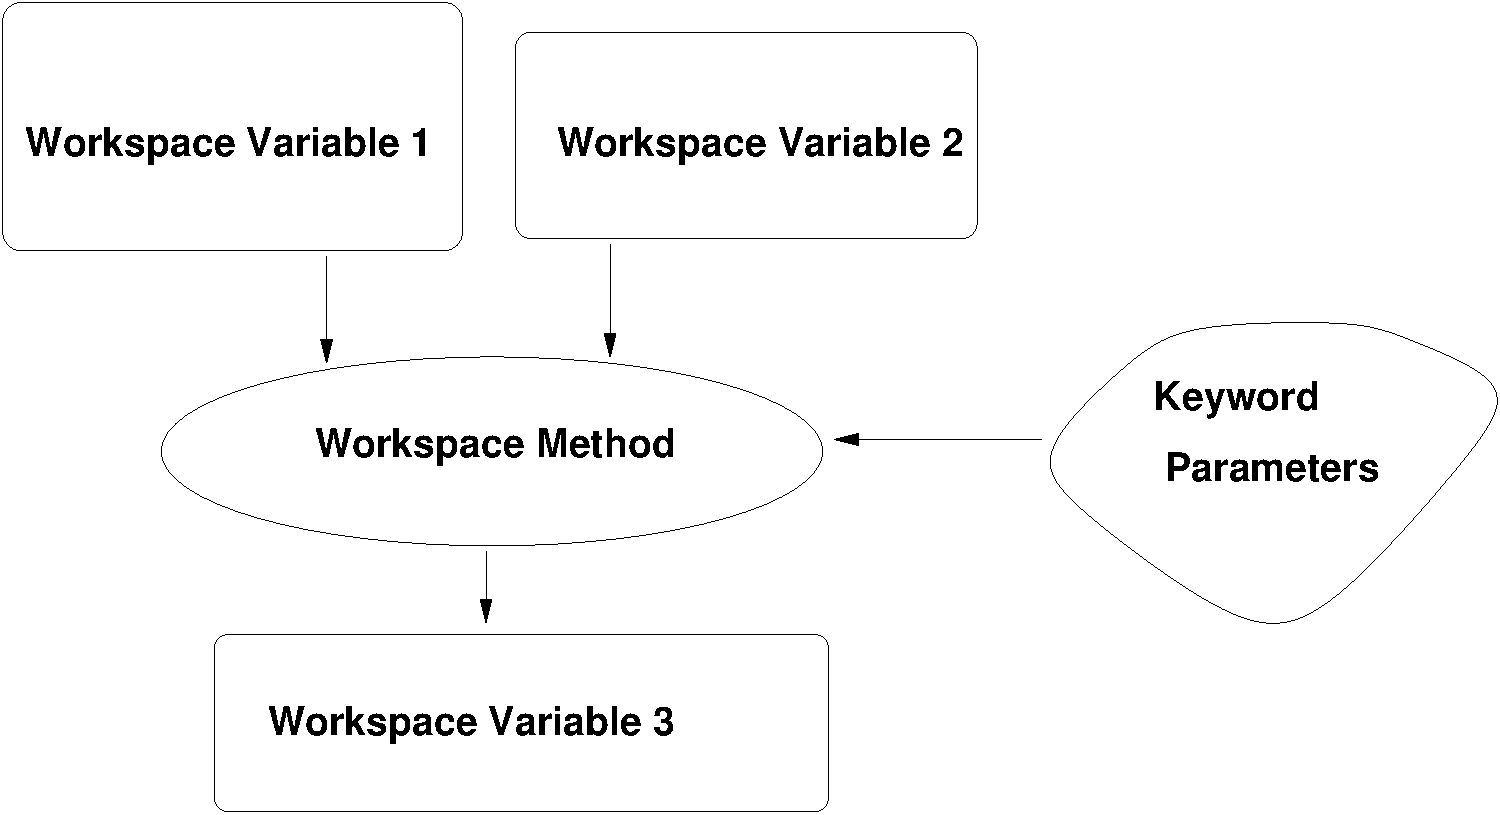
\includegraphics[width=\hsize,draft=false]{concept/method}
    \caption{\textindex{Specific
        workspace methods} act on specific workspace variables to
        generate other specific workspace variables. Additional input
        parameters can be specified as keyword parameters in the
        controlfile.}
    \label{fig:method}
  \end{center}
\end{figure}

It is important to note that the controlfile has a fixed and
well-defined syntax. This syntax is understood by the ARTS parser.
The great advantage of this concept is that it is very easy to add
new workspace variables and new workspace methods. The program has
an internal lookup table which lists all workspace methods, as well
as their input variables, output variables, and keyword
parameters. To add a new method, one just has to add an entry to
this lookup table, and write the code for the method itself. No
further changes to the program are necessary. In particular, no
changes to the program logic or to the parser. How such an extension
can be made practically is described in Section \ref{sec:development}.


\section{Generic Workspace Methods}
%=================================
\label{sec:concept:generic}

Generic methods (Figure \ref{fig:generic_method}) allow the user of
the program even more freedom than specific methods. A generic method
is for example \artsstyle{MatrixSet}, which can be used to set any
workspace variable which is a matrix. For example
\begin{quote}
  \artsstyle{MatrixSet(z\_surface){0.0}}
\end{quote}
will set all elements of \artsstyle{z\_surface} to 0.0 (as long as
\artsstyle{nrows} and \artsstyle{ncols} are set).

\begin{figure}
  \begin{center}
    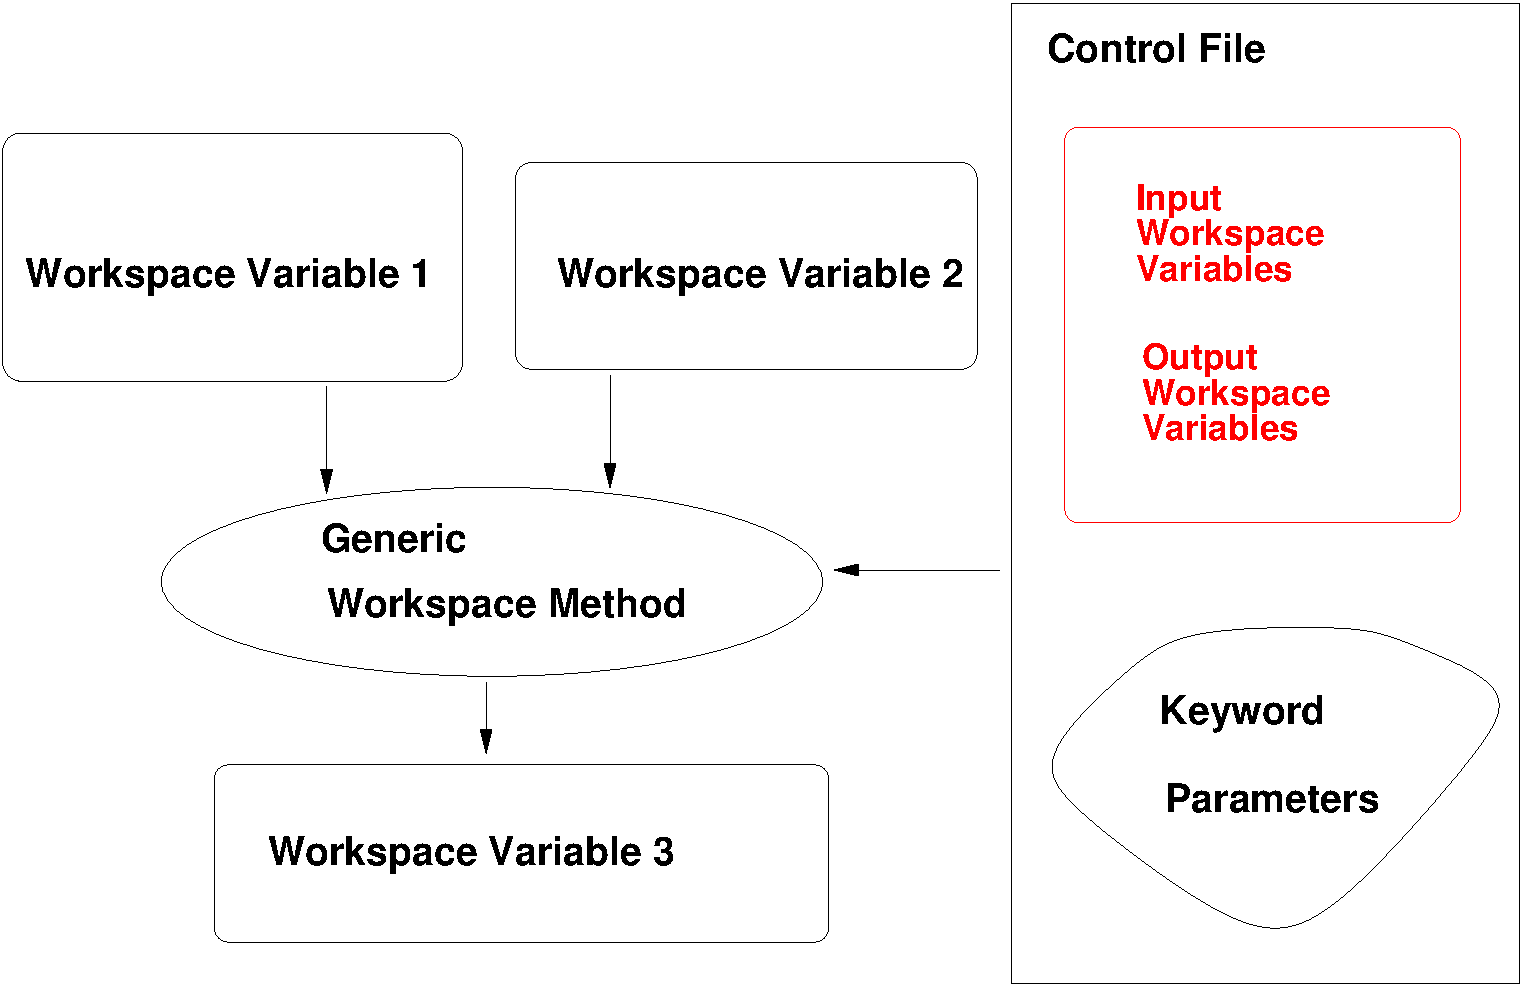
\includegraphics[width=\hsize,draft=false]{concept/generic_method}
    \caption{For \textindex{generic
      workspace methods} the workspace variables to act on are
        specified in the controlfile.}
    \label{fig:generic_method}
  \end{center}
\end{figure}

Some methods are even more flexible, the are super generic. This means
that they can take any workspace variable as input. The most commonly
used such methods are the XML file methods. A workspace variable is
read from a file in this way
\begin{quote}
  \artsstyle{ReadXML(f\_grid)\{"frequency\_grid"\}}
\end{quote}
Generic methods are particularly useful for IO operations like in the
example above. No new IO methods are necessary for new workspace
variables, as long as they are of standard types already known to the
program (for example vectors or matrices). 



\section{Agendas}
%=================================
\label{sec:concept:agendas}

Agendas are a special incarnation of a workspace method. In the
controlfile an arbitrary number of workspace methods can be added to
an agenda. On invocation, the agenda executes its methods one
after the other. The inputs and outputs defined for the agenda must
be satisfied by the invoked workspace methods. E.g., if an agenda
has \artsstyle{f\_grid} in its list of output workspace variables, a
workspace method which generates \artsstyle{f\_grid} must be added to
the agenda in the controlfile.

Even though it is possible to execute agendas directly from the
controlfile with the \artsstyle{AgendaExecute} method, the more common
and intended use case is the internal invocation by other workspace
methods. This adds a grave amount of flexibility to arts. The
\artsstyle{RteStd} method for example calculates (besides other
components) the emission term. Without the means of an agenda, it
would only be possible to use always the same method for the emission
calculation. By the use of an agenda the user can choose between
different methods to calculate the emission and plug them into the
emission agenda in the control file:

{\small
\begin{verbatim}
AgendaSet(emission_agenda){
  emissionPlanck{}
}
\end{verbatim}
}

\noindent
\artsstyle{RteStd} internally calls the \artsstyle{emission\_agenda} and
uses the user selected method for calculating the emission term.



\section{Practical hints}
%=================================
\label{sec:concept:practical}

The subdirectory \fileindex{tests} contains some example controlfiles.
You should study them to learn more about how the program works. You
can also run these controlfiles like this:
\begin{quote}
\begin{verbatim}
  arts TestAbs.arts
\end{verbatim}
\end{quote}
This assumes that you are inside the directory where the controlfiles
are, and that the \artsstyle{arts} executable is in your path.  You can
also run all of the examples, by saying
\begin{quote}
\begin{verbatim}
  make check
\end{verbatim}
\end{quote}

ARTS offers a number of useful command line parameters. In general,
there is a short form and a long form for each parameter. The short
form consists of a minus sign and a single letter, whereas the long
form consists of two minus signs and a descriptive name. To get a full
list, type
\begin{quote}
\begin{verbatim}
  arts -h
\end{verbatim}
\end{quote}
or
\begin{quote}
\begin{verbatim}
  arts --help
\end{verbatim}
\end{quote}
Most useful at the beginning should be the \artsstyle{-d}
(\artsstyle{--describe}), \artsstyle{-m} (\artsstyle{--methods}), \artsstyle{-w}
(\artsstyle{--workspacevariables}), and \artsstyle{-i} (\artsstyle{--input}) flags.
For instance, the \artsstyle{-d} (\artsstyle{--describe}) flag gives you online
documentation for any workspace method or workspace variable. Usage:
\begin{quote}
\begin{verbatim}
  arts -d f_grid
\end{verbatim}
\end{quote}
will print documentation about the workspace variable \artsstyle{f\_grid}, which
happens to be the monochromatic frequency grid.

But what methods and variables are available? You can find out by
typing
\begin{quote}
\begin{verbatim}
  arts -m all
\end{verbatim}
\end{quote}
which will list all workspace methods, or by typing 
\begin{quote}
\begin{verbatim}
  arts -w all
\end{verbatim}
\end{quote}
which will list all workspace variables. As you can see, these lists
are quite long. But you can get more specific information:
\begin{quote}
\begin{verbatim}
  arts -m f_grid
\end{verbatim}
\end{quote}
will give you a list of all methods that can generate the workspace
variable \artsstyle{f\_grid}. Specific and generic methods are listed
separately. Generic methods are in this case all methods producing a
Vector, since \artsstyle{f\_grid} belongs to this group. A similar task is
performed by the \artsstyle{-i} (\artsstyle{--input}) flag, with the difference
that \artsstyle{arts -i f\_grid} will list those methods that require
\artsstyle{f\_grid} as \emph{input}, whereas \artsstyle{arts -m f\_grid} lists
those that produce \artsstyle{f\_grid} as output. Finally,
\begin{quote}
\begin{verbatim}
  arts -w surfaceFlat
\end{verbatim}
\end{quote}
will give you all variables required by the method \artsstyle{abs\_coefCalc}
(the variable \artsstyle{f\_grid} happens to be one of them).

Using these command line parameters, it is easy to build up a
controlfile. The trick is, to start at the end. Say you want to
compute absorption coefficients. First of all, you have to find out
in which workspace variable these are stored. Look at the list
produced by \artsstyle{arts -w all}. You can use \artsstyle{arts -d} to look at
some candidates a bit more closely. This way, you will find out that
\artsstyle{abs\_coef} is the variable you are looking for.

In the next step, you can use \artsstyle{arts -m abs\_coef} to find all methods
that can calculate \artsstyle{abs\_coef}. So, you will find the method
\artsstyle{abs\_coefCalc}. Now you can use \artsstyle{arts -w abs\_coefCalc} to find out the
required input variables of that method. Then you can use the
\artsstyle{-m} flag again, to find the methods producing these variables,
and so on.

%%% Local Variables: 
%%% mode: latex
%%% TeX-master: "uguide"
%%% End: 

%
% To start the document, use
%  \levela{...}
% For lover level, sections use
%  \levelb{...}
%  \levelc{...}
%
\levela{The forward model: concepts, definitions and overview}
 \label{sec:fm_defs}

%
% Document history, format:
%  \starthistory
%    date1 & text .... \\
%    date2 & text .... \\
%    ....
%  \stophistory
%
\starthistory
  020330 & Structure for the chapter fixed, and absorption, compulsory sensor 
           variables and part of RTE sections written by Patrick Eriksson.\\
\stophistory


%
% Symbol table, format:
%  \startsymbols
%    ... & \artsstyle{...} & text ... \\
%    ... & \artsstyle{...} & text ... \\
%    ....
%  \stopsymbols
%
%
\startsymbols
  \Ind           & \artsstyle{i}         & vector/matrix/tensor index        \\
  \aInd{\Lat}    & \artsstyle{i\_alpha}  & the \Ind:th latitude              \\
  \VctLng        & \artsstyle{n}         & vector length or size of matrix/tensor for a dimension \\
  \aVctLng{\Lat} & \artsstyle{n\_alpha}  & length of the latitude grid       \\
  $e_g$          & \artsstyle{e\_ground} & ground emissivity                 \\
  \Prs           & \artsstyle{p}         & pressure                          \\
  \PrsAlt        & \artsstyle{pz}        & pressure altitude                 \\
  \Rds           & \artsstyle{r}         & radius from the centre of the coordinate system         \\
  \Tmp           & \artsstyle{t}         & temperature                       \\
  \Alt           & \artsstyle{z}         & geometrical altitude above the geoid \\
  \Planck        & \artsstyle{source}    & Planck function                   \\
  \Lat           & \artsstyle{alpha}     & latitude                          \\
  \Lon           & \artsstyle{beta}      & longitude                         \\
  \ZntAng        & \artsstyle{psi}       & zenith angle                      \\
  \AzmAng        & \artsstyle{omega}     & azimuthal angle                   \\
  \MpiVct        & \artsstyle{mpi}       & vector with monochromatic pencil beam values \\
  \MsrVct        & \artsstyle{y}         & measurement vector                \\
  \SnsMtr        & \artsstyle{h}         & sensor and data reduction transfer matrix \\
 \label{symtable:fm_defs}     
\stopsymbols



This chapter introduces terms and concepts of ARTS as a forward model,
in contrast to the previous chapter that describes ARTS as a computer
programme. While the content of the previous chapter is specific for
ARTS, as the way to use a forward model programme differ normally
significantly from one implementation to another, this chapter is of
more general nature. Most of the quantities treated here should be
part of any forward model of the same complexity as ARTS, where only
details regarding the definition should differ. The aim of this
chapter is to give an overview of the forward model and to describe
important terms and concepts, in such way that the content of this user
guide can be fully appreciated and that you shall understand how to
construct a control file for your simulation problem.



\levelb{Mathematics}
%==============================================================================
\label{sec:fm_defs:math}

[* A short introduction to the vectors, matrices and tensors should be
found here. It should be described what the terms means, the standard
order in which dimensions are given, how sizes are specified here in
the guide, how different dimensionalities are handled etc.

Vectors, matrices and tensors are indexed using round braces.
It should normally not be needed to specify the size. If you want to
show in what order the dimensions are put into the variable, use the
notation:
\begin{equation}
  \Alt = \Alt(\Prs,\Lat,\Lon)
\end{equation}
If the a special size shall be given, give the size inside square
brackets and spell out that you refer to the size. An example, 
``the matrix describing the geoid has for 1D the size $[1,1]$''.

The concept of rows, columns, pages etc. should be described so a
particular dimension can be identified in a consistent manner.

The indexing is 0-based as in ARTS. *]



\levelb{The atmosphere}
%==============================================================================
\label{sec:fm_defs:atmosphere}


\levelc{Atmospheric dimensionality}
%===================
\label{sec:fm_defs:atmdim}

The structure of the modelled atmosphere can be selected to have
different degree of complexity, the \textindex{atmospheric
  dimensionality}. There exist three levels for the complexity of the
atmosphere, 1D, 2D and 3D, where 1D and 2D can be treated as special
cases of 3D. The significance of these different atmospheric
dimensionalities and the coordinate systems used are described below
in this section. The atmospheric dimensionality is selected by setting
the workspace variable \wsvindex{atmosphere\_dim} to a value between 1
and 3. Variables for which the size depends on the atmospheric
dimensionality are checked, when used, to have a size consistent with
\artsstyle{atmosphere\_dim}. The atmospheric dimensionality is most
easily set by the functions \wsfindex{SetAtmosphere1D},
\wsfindex{SetAtmosphere2D} and \wsfindex{SetAtmosphere3D}.

\begin{description}
  
\item[\textindex{3D}\,\,\,] In this, the most general, case, the
  atmospheric fields vary in all three spatial coordinates, as in a
  true atmosphere. A \textindex{spherical coordinate system} is used where the
  dimensions are radius (\Rds), latitude (\Lat) and longitude (\Lon),
  and a position is given as $(\Rds,\Lat,\Lon)$. With other words, the
  standard way to specify a geographical position is followed.
  However, the way to specify the radial position differs depending on
  the context, which is described in
  Section~\ref{sec:fm_defs:altitudes}. The valid range for latitudes
  is $[-90\degree,+90\degree]$, where +90\degree corresponds to the
  North pole etc. Longitudes are counted from the Greenwich meridian
  with positive values towards the east. Longitudes can have values
  from -360\degree to +360\degree. When the difference between the
  last and first value of the longitude grid is $\geq 360\degree$ then
  the whole globe is considered to be covered. The user must ensure
  that the atmospheric fields for \Lon\ and $\Lon+360\degree$ are
  equal. If a point of propagation path is found to be outside the
  range of the longitude grid, this will results in an error if not
  the whole globe is covered. Otherwise, the longitude is shifted with
  360\degree\ in the relevant direction.
  
\item[\textindex{1D}\,\,\,] A 1D atmosphere can be described as being
  spherically symmetric. The term 1D is used here for simplicity and
  historical reasons, not because it is a true 1D case (a strictly 1D
  atmosphere would just extend along a line). A spherical symmetry
  means that atmospheric fields and the ground extend in all three
  dimensions, but they have no latitude and longitude variation. This
  means that, for example, atmospheric fields vary only as a function
  of altitude and the ground constitutes the surface of a sphere. The
  radial coordinate is accordingly sufficient when dealing with
  atmospheric quantities, but the angular distance between the sensor
  and a point along the propagation path can be of interest, for
  example when determining the cross-link between two satellites (a
  fact that shows that this is not a true 1D case). A polar coordinate
  system is for this reason used when describing propagation paths,
  where the coordinate additional to the radius gives the angular
  distance inside the viewing plane between the sensor and the point
  of interest (see also Section~\ref{sec:ppath:Ppath}). This latter
  coordinate system coincides with the one used for 2D if the sensor
  position is set to be the zero point for the latitudes. A 1D
  atmosphere is shown in Figure~\ref{fig:fm_defs:1d}.
  
\item[\textindex{2D}\,\,\,] In contrast to the 1D and 3D cases, a 2D
  atmosphere extends only inside a plane. A spherical coordinate
  system is accordingly not needed and a polar system\index{polar
    coordinate system}, consisting of a radial and an angular
  coordinate, is used. The 2D case is most likely used for satellite
  measurements where the atmosphere is observed inside the orbit
  plane. The angular coordinate corresponds then to the angular
  distance along the satellite track, but the coordinate is for
  simplicity denoted as the latitude. The zero point for the 2D
  latitude is arbitrary. No lower and upper limit exists for the 2D
  latitude, and this allows that measurements from several subsequent
  orbits can be simulated as one unit. The atmosphere is treated to be
  undefined outside the considered plane. A 2D atmosphere is shown in
  Figure~\ref{fig:fm_defs:2d}.

\end{description}

\begin{figure}[!t]
 \begin{center}
  \includegraphics*[width=0.95\hsize]{Figs/fm_definitions/atm_dim_1d}
  \caption{A schematic cross-section of a 1D atmosphere. The atmosphere is 
    here spherically symmetric. This means that the radius of the
    geoid, the ground and all the pressure surfaces is constant. The
    cloud box extends here from the ground up to the thin solid line
    (no blackbody ground assumed). The upper limit of the cloud box
    coincides always with a pressure surface. }
  \label{fig:fm_defs:1d}  
 \end{center}
\end{figure}
% This figure was produced by the Matlab function mkfigs_atm_dims.

\begin{figure}[!t]
 \begin{center}
  \includegraphics*[width=0.95\hsize]{Figs/fm_definitions/atm_dim_2d}
  \caption{ Schematic of a 2D atmosphere. The radii of the geoid, the ground
    and all the pressure surfaces are for 2D atmospheres allowed to
    have a latitude variation. The limits of the cloud box coincide
    always with grid box boundaries. A blackbody ground is assumed
    here as the cloud box does not extend down to the ground. }
  \label{fig:fm_defs:2d}
 \end{center}
\end{figure}
% This figure was produced by the Matlab function mkfigs_atm_dims.


\levelc{Altitude coordinates}
%===================
\label{sec:fm_defs:altitudes}

\begin{description}
  
\item[Pressure\index{pressure}] The main altitude coordinate is
  pressure. This is most clearly manifested by the fact that the
  vertical atmospheric grid consists of surfaces with equal pressure.
  The vertical grid is consistently denoted as the pressure grid and
  the corresponding workspace variable is called \wsvindex{p\_grid}. The
  choice of having pressure as main altitude coordinate results in
  that atmospheric quantities are retrieved as a function pressure,
  not as a function of geometrical altitude.
  
\item[Pressure altitude\index{pressure altitude}] A basic assumption
  in ARTS is that atmospheric quantities (temperature, geometric
  altitude, species VMR etc.) vary linear with the logarithm of the
  pressure. This corresponds roughly to assuming a linear variation
  with altitude. To obtain a more intuitive unit for the logarithm of
  the pressure, the quantity pressure altitude, \PrsAlt, is
  introduced, and it is defined as
  \begin{equation}
   \PrsAlt = \aPrsAlt{s}\left( \log_{10}(\aPrs{0}) - \log_{10}(\Prs) \right)
   \label{eq:fm_defs:prsalt}
  \end{equation}
  where \aPrsAlt{s} and \aPrs{0} are arbitrary parameters (set in
  \fileindex{arts.h}), but suitably selected in such way that the pressure
  altitude corresponds roughly with the geometrical altitude.  This
  correspondence is achieved if the two parameters are treated as a
  fixed scale height (for decreases of the pressure with a factor of
  10) and the surface pressure, respectively. Values around
  $\aPrsAlt{s}=15.5$~km and $\aPrs{0}=1013$~hPa are suitable for
  simulations dealing with the Earth's atmosphere.
  
\item[Radius\index{radius}] Geometrical altitudes are
  needed to determine the propagation path through the atmosphere etc.
  The main geometrical altitude coordinate is the distance to the
  centre of the coordinate system used, the radius. This is a natural
  consequence of using a spherical or polar coordinate system. The
  radius is used inside ARTS for all geometrical calculations and to
  store the position of the sensor (Section~
  \ref{sec:fm_defs:sensor1}).
  
\item[Geometrical altitude\index{geometrical altitude}] The term
  geometrical altitude signifies here the difference in radius between
  a point and the geoid (Section~\ref{sec:fm_defs:geoid}) along the
  vector to the centre of the coordinate system
  (Equation~\ref{eq:fm_defs:zground}). Hence, the geometrical altitude
  is not measured along the local zenith direction (the normal to the
  reference geoid). Geometrical altitudes are mainly used to
  facilitate the input of the ground altitude, the altitude of the
  pressure surfaces etc. This is the case as these quantities are known
  rather with respect to the geoid than with respect to the Earth's
  centre.

\end{description}


\levelc{Atmospheric grids and fields}
%===================
\label{sec:fm_defs:grids}

As mentioned above, the vertical grid of the atmosphere consists of a
set of layers with equal pressure, the pressure grid
(\wsvindex{p\_grid}).  This grid must of course always be specified.
It is not allowed that there is an altitude gap between the ground and
the lowermost pressure surface.  That is, the ground pressure must be
smaller than the pressure of the lowermost vertical grid surface. On
the other hand, it is not necessary to match the ground and the first
pressure surface, the pressure grid can extend below the ground level.
The upper end of the pressure grid gives the practical upper limit of
the atmosphere as vacuum is assumed above. With other words, no
absorption and refraction take place above the uppermost pressure
surface.

A \textindex{latitude} grid (\wsvindex{lat\_grid}) must be specified
for 2D and 3D.  For 2D, the latitudes shall be treated as the angular
distance along the orbit track, as described above in
Section~\ref{sec:fm_defs:atmdim}.  The latitude angle is throughout
calculated for the vector going from the centre of the coordinate
system to the point of concern. Hence, the latitudes here correspond
to the definition of the geocentric latitude, and not geodetic
latitudes (see Section~\ref{sec:ppath:geoid}). This is an accordance
to the definition of geometric altitudes found above.  For 3D, a
\textindex{longitude} grid (\wsvindex{lon\_grid}) must also be specified.
Valid ranges for latitude and longitude values are given in
Section~\ref{sec:fm_defs:atmdim}.

The atmosphere is treated to be undefined outside the latitude and
longitude ranges covered by the grids, if not the whole globe is
covered. This results in that a propagation path is not allowed to
cross a latitude or longitude end face of the atmosphere, if such
exists, it can only enter or leave the atmosphere through the top of
the atmosphere (the uppermost pressure level). See further
Section~\ref{sec:fm_defs:ppaths}. The volume (or area for 2D) covered
by the grids is denoted as the \textindex{model atmosphere}.

If the longitude and latitude grids are not used for the selected
atmospheric dimensionality, then the longitude grid (for 1D and 2D)
and the latitude grid (for 1D) must be set to be empty, but when
dealing with the size of variables the grid length shall be treated to
be one. For example, the matrix describing the geoid (see
Section~\ref{sec:fm_defs:geoid}) has for 1D the size $[1,1]$.

The basic atmospheric quantities are represented by their values at
each crossing of the involved grids (indicated by thick dots in
Figure~\ref{fig:fm_defs:2d}), or for 1D at each pressure surface
(thick dots in Figure~\ref{fig:fm_defs:1d}). This representation is
denoted as the field\index{atmospheric field} of the quantity. The
field must, at least, be specified for the geometric altitude of the
pressure surfaces (\wsvindex{z\_field}), the temperature
(\wsvindex{t\_field}) and considered atmospheric species
(\artsstyle{vmr\_field}).  The fields are assumed to be piece-wise
linear functions vertically (with pressure altitude as the vertical
coordinate, Section~\ref{sec:fm_defs:altitudes}), and along the
latitude and longitude edges of 2D and 3D grid boxes. For points
inside 2D and 3D grid boxes, multidimensional linear interpolation is
applied (that is, bilinear interpolation for 2D etc.). Note especially
that this is also valid for the field of geometrical altitudes
(\artsstyle{z\_field}). Fields are rank-3 tensors. For example, the
temperature field is $T=T(\Prs,\Lat,\Lon)$. That means each field is
like a book, with one page for each pressure grid point, one row for
each latitude grid point, and one column for each longitude grid
point. In the 1-D case there is just one row and one column on each
page.



\levelc{The geoid and the ground}
%===================
\label{sec:fm_defs:geoid}

The \textindex{geoid} is an imaginary surface used as a
reference when specifying the ground altitude and the altitude
of pressure surfaces. Any shape of the geoid is allowed but a smoothly
varying geoid is the natural choice, with the centres of the geoid and
the coordinate system coinciding. The geoid should normally be set to
the reference ellipsoid for some global geodetic datum, such as
WGS-84. For further reading on geoid ellipsoids and WGS-84, see
Section~\ref{sec:ppath:geoid}.

Inside ARTS, the geoid is represented as a matrix
(\wsvindex{r\_geoid}), holding the geoid radius, \aRds{\odot}, for
each crossing of the latitude and longitude grids,
$\aRds{\odot}=\aRds{\odot}(\Lat,\Lon)$. The geoid is not defined
outside the ranges covered by the latitude and longitude grids, with
the exception for 1D where the geoid by definition is a full sphere.
The ground altitude, \aAlt{g}, is given as the geometrical altitude
above the geoid. The radius for the ground is accordingly
\begin{equation}
  \aRds{g} = \aRds{\odot} + \aAlt{g}
 \label{eq:fm_defs:zground}
\end{equation}
As described in
Section~\ref{sec:fm_defs:grids}, it is not allowed that there is a gap
between the ground and the lowermost pressure level.

The ARTS variable for the \textindex{ground altitude}
(\wsvindex{z\_ground}) is a matrix of the same size as the geoid
matrix. For 1D, the ground is a sphere by definition (as the geoid),
while for 2D and 3D any shape is allowed and a rough model of the
ground topography can be made. For example, for limb sounding into the
troposphere, it could be of importance to capture the intersection of
the antenna beam by the Himalayas, and maybe other mountain ridges.
However, it should be noted that ground reflections are treated in a
simplified manner and accurate results cannot be expected beside when
some conditions are fulfilled (see
Section~\ref{sec:fm_defs:groundrefl}).

The temperature of the ground\index{ground temperature} (\aTmp{g}) is
described by the matrix \wsvindex{t\_ground} that has the same size as
\artsstyle{r\_geoid} and \artsstyle{z\_ground}. The \textindex{ground
  emission} is described by the variable \wsvindex{e\_ground}, holding
the ground emission factor $(e_g)$ of the ground, as a function of
frequency for each latitude/longitude position. This workspace
variable is a tensor of order 3, $e_g = e_g(\Frq,\Lat,\Lon)$. The
emission from the ground is $e_g(\Frq)\Planck(\Frq,\aTmp{g})$, where
\Planck\ is the Planck blackbody function. That is, the emissivity is
a value between 0 and 1, where 0 means that the ground has no
emissivity, and for $e_g=1$ the ground acts as a blackbody for that
particular frequency.

\begin{description}
\item[Blackbody ground\index{blackbody ground}] The ground can be
  treated to act as a blackbody, which is of importance for the cloud
  box and determination of propagation paths
  (Section~\ref{sec:fm_defs:cloudbox} and \ref{sec:fm_defs:ppaths},
  respectively). This feature is selected by the variable
  \wsvindex{blackbody\_ground}. For consistency reasons,
  \artsstyle{e\_ground} is demanded to only contain ones when
  \artsstyle{blackbody\_ground} is set to 1, but the size $[1,1,1]$ is
  then allowed also for 2D and 3D to save memory. The ground is only
  treated to be a blackbody when \artsstyle{blackbody\_ground} is set
  to 1. If \artsstyle{e\_ground} only contains 1, but
  \artsstyle{blackbody\_ground} is set to 0, the calculations will be
  performed such as the radiation is reflected by the ground. A
  blackbody ground is most easily selected by the function
  \wsfindex{SetBlackbodyGround}.
\end{description}


\levelc{The cloud box}
%===================
\label{sec:fm_defs:cloudbox}

In order to save computational time, scattering calculations are
limited as far as possible to the part of the atmosphere containing
clouds and other scattering objects. The atmospheric region in which
scattering shall be considered is denoted as the \textindex{cloud box},
and it is discussed here as it acts as an additional atmospheric limit
when calculating propagation paths (see
Section~\ref{sec:fm_defs:rte}).

The cloud box is defined in such way that a propagation path entering
the cloud box at one position has not crossed the cloud box boundary
at any other location (remember that there is no scattering outside
the cloud box). This requires in general that the lower limit of the
cloud box is the ground. This is the case as if there is a gap between
the ground and the cloud box, paths entering the cloud box from below
after a ground reflection have passed through the cloud box on the way
down, at least for propagations paths close to nadir. However, with a
blackbody ground (Section~\ref{sec:fm_defs:geoid}), there is
effectively no ground reflection
(Section~\ref{sec:fm_defs:groundrefl}) and a gap below the cloud box
is allowed.

The cloud box is defined to be rectangular in the used coordinate
system, with limits exactly at points of the involved grids. This
means, for example, that the vertical limits of the cloud box are two
pressure surfaces. If the ground is not a blackbody, the lower limit
must be set to the lowest pressure surface (index 0). For 2D, the
angular extension of the cloud box is between two points of the
latitude grid (Figure~\ref{fig:fm_defs:2d}), and likewise for 3D but
then also with a longitude extension between two grid points.  The
latitude and longitude limits for the cloud box cannot be placed at
the end points of the corresponding grid as it must be possible to
calculate the incoming intensity field. The cloud
box is activated by setting the variable \wsvindex{cloudbox\_on} to 1. The
limits of the cloud box are stored in \wsvindex{cloudbox\_limits}.

There exists in fact a small risk for 2D or 3D, and with a reflecting
ground, that a propagation path into the cloud box has earlier crossed
the box boundaries. This can happen for propagation paths close to the
nadir direction and if the ground is tilted in such way that the
surface of the ground points towards the cloud box. The first crossing
of the cloud box is neglected for such cases, the cloud box is simply
turned off when determining the radiation field going into the cloud
box.


\levelb{Absorption and refractive index}
%==============================================================================
\label{sec:fm_defs:absorption}

[* Considerations for the calculation of absorption and refractive
index ...  Tags, line-by-line, absorption models etc. The old
\artsstyle{f\_mono} should be called \artsstyle{f\_mono}, or? (Note that I
have used the name \wsvindex{f\_grid} elsewhere.)*]



\levelb{Compulsory sensor and data reduction variables}
%==============================================================================
\label{sec:fm_defs:sensor1}

The instrument that detects the simulated radiation is denoted as the
sensor\index{sensor, the}. The forward model is constructed in such
way that a sensor must exists. For cases when only monochromatic
pencil beam radiation is of interest, the positions and directions for
which the radiation shall be calculated are given by specifying an
imaginary sensor with infinite frequency and angular resolution. The
workspace variables for the sensor that always must be specified are
\artsstyle{sensor\_pos}, \artsstyle{sensor\_los},
\artsstyle{sensor\_pol}, \artsstyle{antenna\_dim},
\artsstyle{psi\_block\_grid}, \artsstyle{omega\_block\_grid} and
\artsstyle{Hb}. These variables are presented separately below in this
section. The discussion of sensor workspace variables is continued in
Section~\ref{sec:fm_defs:sensor2}. The Section~\ref{sec:fm_defs:rte}
gives further insights in how the sensor is treated in ARTS.


\levelc{Sensor position\index{sensor position}}
%===================
\label{sec:fm_defs:sensorpos}

The observation positions of the sensor are stored in
\wsvindex{sensor\_pos}. This is a matrix where each row corresponds to a
sensor position. The number of columns in the matrix equals the
atmospheric dimensionality (1 column for 1D etc.). The columns of the
matrix (from first to last) are radius, latitude and longitude.
Accordingly, row $i$ of \artsstyle{sensor\_pos} for a 3D case is
$(\aRds{i},\aLat{i},\aLon{i})$. The sensor position can be set to any
value, but the resulting propagation paths (also dependent on
\artsstyle{sensor\_los}) must be valid with respect to the model atmosphere
(see Section~\ref{sec:fm_defs:ppaths}). An obviously incorrect choice
is to place the senor below the ground altitude. If the sensor is
placed inside the model atmosphere, any sensor line-of-sight is
allowed, this including the cases that the sensor is placed on the
ground looking down, and that the sensor is placed on the boundary of
the cloud box and looks into the box. The sensor can also be placed
inside the cloud box.

The fact that the sensor position can be given any value results in
that the radius must be used in \artsstyle{sensor\_pos}, in contrast
to \artsstyle{z\_ground} and \artsstyle{z\_field} where the altitude
above the geoid is applied. This is the case as the sensor can for 2D
and 3D be placed outside the covered latitude and longitude ranges,
thus outside the defined geoid and the geometrical altitude is
undefined. See Section~[**] for hints on how to simply set the sensor
position.

The sensor is treated to be motionless when calculating the spectrum,
or spectra, for each given observation position. One or several
spectra can be calculated for each position as described in
Section~\ref{sec:fm_defs:seqsandblocks}.


\levelc{Line-of-sight\index{line-of-sight}}
%===================
\label{sec:fm_defs:los}

The viewing direction of the sensor, the line-of-sight, is described
with two angles, the zenith angle (\ZntAng) and the azimuth angle
(\AzmAng). The zenith angle exists for all atmospheric
dimensionalities, while the azimuthal angle is defined only for 3D.
The term line-of-sight is not only used in connection with the sensor,
it is also used to describe the local propagation direction along the
path taken by the observed radiation
(Section~\ref{sec:fm_defs:ppaths}).  The zenith and azimuthal angles
are defined identical in these two contexts. This is expected as the
position of the sensor is the end point of the propagation path. The
line-of-sight of \textindex{propagation path}s is defined in the
direction the radiation travels to reach the sensor, while the sensor
line-of-sight is the direction the antenna is pointed to receive the
radiation. This means that the sensor and path line-of-sights (at the
sensor) are parallel but go in opposite directions. As a true sensor
has a limited spatial resolution (described by the antenna pattern),
theoretically there are an infinite number of line-of-sights
associated with the sensor, but in the forward model spectra are only
calculated for a discrete set of directions. If a sensor line-of-sight
is mentioned without any comments, it refers to the direction in which
the centre of the antenna pattern is directed.

\begin{figure}[!t]
 \begin{center}
  \begin{minipage}[c]{0.4\textwidth}
   \begin{picture}(100,110)
    \put(10,10){\vector(0,1){100}}
    \put(0,114){zenith}
    \put(10,10){\vector(1,0){100}}
    \put(97,0){north}
    \put(10,10){\vector(-1,0){20}}
    \put(-20,0){south}
    \put(10,10){\vector(1,1){80}}
    \put(65,93){line-of-sight}
    \put(10,10){\arc{40}{-1.5708}{-0.7854}}
    \put(18,34){\ZntAng}
    \dottedline(90,90)(90,35)(10,10)
    \drawline(85,33.4)(85,38.4)(90,40)
    \put(10,10){\arc{50}{-.3}{0}}
    \put(38,12){\AzmAng}
   \end{picture}
  \end{minipage}%
  \begin{minipage}[c]{0.50\textwidth}
   \caption{Definition of zenith angle, \ZntAng, and azimuthal angle, 
       \AzmAng, for a line-of-sight. The figure shows a line-of-sight
       with a negative azimuthal angle.}
   \label{fig:fm_defs:los}
  \end{minipage}
 \end{center}
\end{figure}           
 
The \textindex{zenith angle}, \ZntAng, is simply the angle between the
line-of-sight and the zenith direction (Figure~\ref{fig:fm_defs:los}).
The valid range for 1D and 3D cases is $[0,180\degree]$. In the case
of 2D, zenith angles down to -180\degree are also allowed, where the
distinction is that positive angles mean a viewing direction is
towards higher latitudes, and vice versa. It should be mentioned that
the zenith and nadir directions are here defined to be along the line
passing the centre of the coordinate system and the point of concern
(Section~\ref{sec:ppath:geoid}). A nadir observation,
$\ZntAng=180\degree$, is thus a measurement towards the centre of the
coordinate system. The maximum absolute value of a zenith angle is
180\degree. For 1D and 3D, positive and negative zenith angles are
treated identically, while for 2D a distinction is made.

The \textindex{azimuthal angle}, \AzmAng, is given with respect to the
\textindex{meridian plane}, that is, the plane going through the north
and south poles of the coordinate system $(\Lat=\pm90\degree)$ and the
sensor. The valid range is $[-180\degree,180\degree]$ where angles are
counted clockwise and 0\degree means that the viewing or propagation
direction is north-wise.  Hence, +90\degree means that the direction
of concern goes eastward.

The line-of-sight for propagation paths is discussed further in
Section~\ref{sec:fm_defs:ppaths}. The sensor line-of-sights are stored in
\wsvindex{sensor\_los}. This workspace variable is a matrix, where the
first column holds zenith angles and the second column is azimuthal
angles. For 1D and 2D there is only one column in the matrix, while
for 3D a row $i$ of the matrix is $(\aZntAng{i},\aAzmAng{i})$. The
number of rows for \artsstyle{sensor\_los} must be the same as for
\artsstyle{sensor\_pos}.


\levelc{Sensor polarisation\index{sensor polarisation}}
%===================
\label{sec:fm_defs:sensorpol}

[* How shall this be handled? Can a transfer matrix be used?
\wsvindex{sensor\_pol} *]


\levelc{Sensor characteristics and data reduction}
%===================
\label{sec:fm_defs:sensorchar}

Sensor characteristics\index{sensor characteristics} is used here as a
comprehensive term for the response of all sensor parts, beside
polarisation effects, that affect how the field of monochromatic
pencil beam intensities are translated to the recorded spectrum. For
example, the antenna pattern, the side-band filtering and response of
the spectrometer channels are normally the most important
characteristics for a microwave heterodyne radiometer. Any processing
of the spectral data that takes place before the retrieval is denoted
as \textindex{data reduction}. The most common processing is to represent
the original spectra with a smaller set of values, that is, a
reduction of the data size. The most common data reduction techniques
is binning and Hotelling transformation by an eigenvector expansion
(Section~[**]).

The influence of sensor characteristics and data reduction is in ARTS
incorporated by transfer matrices\index{sensor transfer matrix}, as
described in Section~\ref{sec:formalism:sensor}. The application of
these transfer matrices assumes that each step is a linear operation,
which should be the case for the response of the parts of a well
designed instrument. Non-linear data reduction is handled by special
workspace functions.

The creation of sensor and data reduction transfer matrices is not
(yet?) included in ARTS and no workspace variables exist to describe
the individual sensor parts etc. The sensor and data reduction are
described as a series of units, each having its own transfer matrix.
There is only one compulsory transfer matrix and it is \aSnsMtr{b}
(\wsvindex{Hb}), where the subscript $b$ stands for block (see further
Section~\ref{sec:fm_defs:seqsandblocks}). There are several workspace
variables associated with this transfer matrix where
\wsvindex{antenna\_dim}, \wsvindex{psi\_block\_grid} and
\wsvindex{omega\_block\_grid} are the compulsory ones.

The variable \artsstyle{antenna\_dim} gives the dimensionality of the
antenna pattern\index{antenna pattern dimensionality}, where the
options are 1 and 2, standing for 1D and 2D, respectively. A 1D
antenna dimensionality means that the azimuthal extension of the
antenna pattern is neglected, there is only a zenith angle variation
of the response. A 2D antenna pattern is converted to a 1D pattern by
integrating the azimuthal response for each zenith angle. ARTS handles
not yet 2D antenna patterns, the only allowed choice for
\artsstyle{antenna\_dim} is 1, and the variable
\artsstyle{omega\_block\_grid} has yet no importance (but it must be
initiated, to be empty, before calling \artsstyle{rteCalc}). The
presentation below assumes that the 2D option is implemented.

For each sensor position, a number of monochromatic pencil beam
spectra are calculated. The monochromatic frequencies are given by
\artsstyle{f\_grid} (Section~\ref{sec:fm_defs:absorption}). The pencil
beam directions are obtained by summing the line-of-sight angles
(\artsstyle{sensor\_los}) for the position and the values of
\artsstyle{psi\_block\_grid} and \artsstyle{omega\_block\_grid}. For
example, pencil beam zenith angle $i$ is calculated as
\begin{equation}
  \aZntAng{i} = \aZntAng{0} + \Delta\aZntAng{i}
  \label{eq:fm_defs:psi_grid}
\end{equation}
where \aZntAng{0} is the sensor line-of-sight for the position of
concern and $\Delta\aZntAng{i}$ is value $i$ of
\artsstyle{psi\_block\_grid}.  With other words,
\artsstyle{psi\_block\_grid} and \artsstyle{omega\_block\_grid} give
the grid (relative to the sensor line-of-sight) for the calculation of
the intensity field that will be weighted with the antenna response.
For cases with 1D antenna patterns, \artsstyle{omega\_block\_grid}
must be set to be an empty vector.


\levelc{Measurement sequences and blocks}
%===================
\label{sec:fm_defs:seqsandblocks}

The series of observations modelled by the simulations is denoted as
the \textindex{measurement sequence}. That is, a measurement sequence
covers all spectra recorded at all considered sensor positions
(\artsstyle{sensor\_pos}). A measurement sequence consists of one or several
\textindex{measurement block}s. The observations inside the various
blocks differ only with an off-set of the line-of-sight, all other
factors should be common for all blocks. A block can be treated as a
measurement cycle that is repeated, an integer number of times, to
form the measurement sequence.  The measurement blocks correspond
normally to each unique sensor position of the sequence.

A measurement block cover one or several recorded spectra, depending
on the measurement conditions and the atmospheric dimensionality. A
block can consists of several spectra when there is no effective
motion of the sensor with respect to the atmospheric fields. It should
be noted that for 1D cases, a motion along a constant radius has no
influence on the simulated spectra as the same atmospheric fields are
seen for a given viewing direction. It is favourable, if possible, to
handle all spectra as a single block, instead of using a block for
each sensor position. This is the case as the antenna patterns for the
different line-of-sights are normally overlapping and a pencil beam
spectrum can be used in connection with several measurement spectra to
estimate the intensity field. If a measurement sequence is divided
into several blocks even if a single block would be sufficient, pencil
beam spectra for basically identical propagation paths can be
calculated several times, which of course is unnecessary. To
summerise, for cases when the sensor is not in motion, or with a 1D
atmosphere and a sensor not moving vertically, the aim should be to
use a single block for the measurement sequence.

If not a single block is used, the standard option should be that the
blocks cover one spectrum each. There could exist reasons to select an
intermediate solution, to let the extent of the blocks be several
spectra (but not the full measurement sequence). This could be the
case when the atmospheric dimensionality is 2D or 3D, and the sensor
is moving but the movement during some subsequent spectra can be
neglected. If this can be done must be judged by comparing the
movement of the satellite during the extent of the considered block
size and the spatial resolution, in the direction of the movement, that
is hoped to be achieved. If this intermediate solution shall be an
option, the difference in zenith and azimuthal angles between the
spectra must be the same for all blocks, otherwise \aSnsMtr{b} cannot
be applied for all blocks as done in Equation~\ref{eq:fm_defs:measseq}.

For each block, pencil beam spectra are calculated for the
line-of-sights obtained when summing \wsvindex{sensor\_los} and
\wsvindex{psi\_block\_grid} (and possibly
\wsvindex{omega\_block\_grid}), as described in
Section~\ref{sec:fm_defs:sensorchar}. The pencil beam spectra for each
line-of-sight are appended vertically to form a common vector,
\aMpiVct{b}. Values are put in following the order in
\artsstyle{f\_grid}. Hence, the frequencies for this vector are
\begin{equation}
  \aMpiVct{b} = 
  \left[ \begin{array}{c} 
     \left[
          \begin{array}{c} \aFrq{1}\\\vdots\\\aFrq{{n_\Frq}} \end{array} 
     \right] \\
     \vdots \\
     \left[
          \begin{array}{c} \aFrq{1}\\\vdots\\\aFrq{{n_\Frq}} \end{array} 
     \right]
     \end{array} \right]
  \label{eq:fm_defs:freqs_of_ib}
\end{equation}
where \aFrq{i} is element $i$ of \artsstyle{f\_grid} and $n_\Frq$ the length of
the same vector. The order of the angles inside \artsstyle{psi\_block\_grid}
and \artsstyle{omega\_block\_grid} is followed when looping the pencil beam
directions, where the zenith angle direction is the innermost loop.
That is, for 2D antenna patterns all zenith angles are looped for the
first azimuthal angle etc. 

The transfer matrix \aSnsMtr{b} is applied on each \aMpiVct{b} and the
results are appended vertically, following the order of the positions
in \artsstyle{sensor\_pos}
\begin{equation}
  \MsrVct = \left[ \begin{array}{c} \aSnsMtr{b}\aMpiVct{{b,1}} \\ 
                                    \aSnsMtr{b}\aMpiVct{{b,2}} \\
                                    \vdots                     \\
                                    \aSnsMtr{b}\aMpiVct{{b,n}} 
            \end{array} \right]
  \label{eq:fm_defs:measseq}
\end{equation}
where \MsrVct\ is defined in Equation~\ref{eq:formalism:fm} and $1$
indicates the first sensor position etc. This equation shows that
\wsvindex{Hb} shall contain at least a description of the antenna
response. The matrix \artsstyle{Hb} can also cover other sensor
characteristics and data reduction if the features of concern are
common for all measurement blocks. If this is not the case, those
features must be handled by the other existing transfer matrices or, by
other means, as described in Section~\ref{sec:fm_defs:howtomeasseq}.

As the sensor line-of-sight and block grid values are just added,
there is an ambiguity of the line-of-sight. It is possible to apply a
constant off-set to the line-of-sights, if the block grids are
corrected accordingly. For example, if the simulations deal with limb
sounding and a 1D atmosphere, where normally a single block should be
used despite a number of spectra are recorded, it could be practical
to set the line-of-sight to the viewing direction of the uppermost or
lowermost spectrum, and the zenith angles in \artsstyle{psi\_block\_grid}
will not be centred around zero which is the case when the ``true''
line-of-sight is used.

It should be noted that the compulsory sensor variables give no
information about the content of the obtained \MsrVct, as it is not
clear which parts and features the block transfer matrix covers. If
\artsstyle{Hb} only incorporates the antenna pattern, the result is a set
of hypothetical spectra corresponding to a point inside the sensor. On
the other hand, if \artsstyle{Hb} includes the whole of the sensor and an
eigenvector data reduction, the result is not even a spectrum is
traditional way, it is just a row of coefficients with a vague
physical meaning. To handle quantities appearing at a stage between
monochromatic pencil beam intensities and the final representation of
the measurements (where the total transformation can involve more
steps than the multiplication with \artsstyle{Hb}), additional sensor
variables must be introduced, as described in
Section~\ref{sec:fm_defs:sensor2}.


\levelb{Clear sky radiative transfer}
%==============================================================================
\label{sec:fm_defs:rte}

\newcommand{\Int}{{\bf I}}
\newcommand{\Ext}{{\bf K}}
\newcommand{\Abs}{{\bf a}}
\newcommand{\Sca}{{\bf Y}}
\newcommand{\Dir}{{\bf n}}
\newcommand{\Path}{{\bf s}}
%\newcommand{\Planck}{{\bf B}}
\newcommand{\Freq}{\nu}
\newcommand{\Dep}{(\Dir,\Freq)}

\startsymbols
  \Ind           & -                 & vector/matrix/tensor index           \\
  \Int           & 
 \label{symtable:fm_defs_rt}     
\stopsymbols

% STEFAN, you should have a look at the file symbol_defs. The quantities for
% which you have defined commands should be of general interest and they should
% then be included in that file. For example, there are already macros for
% frequency (\Frq and \aFrq{i}).
%
% I see that you use a capital I for the intensity Stokes vector. I have so
% far (and I don't think there are any exceptions AUG) used lower case letters
% for vectors and upper case for matrices. I would be happy if we could stick
% to this rule, which I think is a standard way to keep matrices and vectors
% separated. Note the macro \MpiVct in symbol_defs.
%
% I just put in a macro for Planck, but then the scalar version. The Planck
% function here is really not a scalar? If not, maybe you can introduce the
% macro \VctPlanck? But what symbol should be used? Lower case b is already
% occupied.
%
% I also think that you should put ''your'' symbols in the table found at the
% start of the section as it is valid for the whole chapter. 
%
% Patrick

\levelc{Radiative transfer equation and important quantities}

The radiative transfer equation in the absence of cloud particles is
\citep{mishchenko00:_light_scatt_nonsp_partic}: 

\begin{equation}
  \label{eq:rte_4stokes_no_scat}
  \frac{d\Int\Dep}{d\Path} = - \Ext\Dep \Int\Dep + \Abs\Dep\Planck(T)
\end{equation}
where the meaning of the quantities in this equation is as follows:

The specific intensity vector $\Int$



 where $I$ is the monochromatic pencil beam intensity, $l$ distance
 along the line of sight (LOS), $l_1$ the point of the considered part
 of the LOS furthest away from the sensor, $l_2$ the closest point of
 the LOS, $I_1$ the intensity at $l_1$, $\kappa$ the total absorption
 along the LOS and $\sigma$ the source function.

[* Please consider also transmission measurements. *]


\levelc{Calculation procedure}
%===================
\label{sec:fm_defs:calcproc}

The overall structure of the part solving the radiative transfer
equation is fixed. The corresponding workspace function is
\wsfindex{rteCalc}. The calculation procedure of \artsstyle{rteCalc} is
outlined in Algorithm~\ref{alg:fm_defs:rteCalc}. For further details
of each calculation step, see the indicated equation or section.

Two types of spectra can be produced, emission and transmission
spectra. A transmission spectrum means that emission of the atmosphere
and the ground is neglected. This can be done if the measurements are
performed against a sufficient strong source, such as the sun. The
background source is not included in the simulations, the output is
instead the transmission through the atmosphere (in form of the
optical thickness, see below). The type of spectra is selected by the
workspace variable \wsvindex{emission\_on}. In some cases it is of interest
to have both the emission and the transmission spectra at hand
simultaneously. This is achieved by [* How? Can we have optional
output parameters? *]. Weighting functions are only calculated for the
option selected by \artsstyle{emission\_on}.

The primary unit for emission spectra, the unit of \aMpiVct{b} in
Equation~\ref{eq:fm_defs:measseq}, is [W/(Hz$\cdot$m$^2\cdot$sr)].
The emission intensity corresponds directly with the definition of the
Planck function in Equation~[**], no scaling terms are applied.
Conversion to brightness temperature is treated in Section~[**].  The
transmission is provided as the optical thickness (Equation~[**]).
The optical thickness includes the absorption of the ground if there
is a ground reflection along the propagation path.

The function \artsstyle{rteCalc}, beside providing atmospheric spectra,
performs also the calculation of weighting functions for atmospheric
variables where analytical expressions are used. The core of these
calculations follows Algorithm~\ref{alg:fm_defs:rteCalc}, but is not
considered here for simplicity. Weighting functions are treated in
Section~\ref{sec:fm_defs:wfs}.

\begin{algorithm}[!t]
 \begin{algorithmic}
  \IF[{Section \ref{sec:fm_defs:scattering}}]{cloud box is turned on}
   \STATE{determine the intensity field inside the cloud box}
  \ENDIF
  \STATE{allocate memory for the measurement vector, \MsrVct}
  \COMMENT{Equation \ref{eq:formalism:fm}}
  \FORALL{sensor positions}
   \STATE{allocate memory for the vector \aMpiVct{b}}
   \COMMENT{Equation \ref{eq:fm_defs:freqs_of_ib}}
   \FORALL[Section \ref{sec:fm_defs:seqsandblocks}]
                                    {pencil beam directions of the block}
    \STATE{determine the propagation path}
    \COMMENT{Section \ref{sec:fm_defs:ppaths}}
    \STATE{initialise the vector \MpiVct\ with the radiative background}
    \COMMENT{Section \ref{sec:fm_defs:ppaths}}
    \FORALL{steps along propagation path}
     \STATE{update \MpiVct\ following Equation [**]}
     \IF{at a point of ground reflection}
      \STATE{update \MpiVct\ following Equation [**]}
     \ENDIF
    \ENDFOR
    \STATE{copy \MpiVct\ to correct part of \aMpiVct{b}}
   \ENDFOR
   \STATE{put the product \aSnsMtr{b}\aMpiVct{b} in correct part of \MsrVct}
  \ENDFOR
 \end{algorithmic}
 \caption{Outline of the clear sky radiative transfer calculations. Only
   calculation of emission spectra is treated here.
   Optical thicknesses and weighting functions are
   determined in parallel, if selected, following the same scheme.}
 \label{alg:fm_defs:rteCalc}
\end{algorithm}


\levelc{Propagation paths}
%===================
\label{sec:fm_defs:ppaths}

A pencil beam path through the atmosphere to reach a specified
position from a specified line-of-sight is denoted as the
\textindex{propagation path}. The forward direction of the propagation
paths is towards the position for which the radiative intensity will
be calculated. It should be noted that with scattering there exist an
infinite number of propagation paths for a given combination of
observation point and line-of-sight.

Propagation paths are described by a set of points on the path, and
the distance along the path between the points. These quantities, and
a number of auxiliary variables, are stored together in a structure
described in Section~[**]. The path points are primarily placed at the
crossings of the path with the atmospheric grids (\artsstyle{p\_grid},
\artsstyle{lat\_grid} and \artsstyle{lon\_grid}). A path point is
also placed at the sensor if it is placed inside the atmosphere.
Ground reflections and tangent points are also included if such exist.
There exists also the possibility to set an upper limit for the
distance along the path between the points by the workspace variable
\wsvindex{ppath\_lmax}. If \artsstyle{ppath\_lmax} is set to a value $\leq 0$
then no points are added to the path, otherwise points are included to
fulfil the length criterion.

The propagation paths are determined basically by starting at the
sensor and following the path backwards by some \textindex{ray tracing}
technique.  If the sensor is placed above the model atmosphere,
geometrical calculations are used (as there is no refraction in space)
to find the crossing between the path and the top of the atmosphere
where the ray tracing then starts. If there is no cloud box and the
ground not acts as a blackbody, the starting point of the propagation
paths is always found at the top of the atmosphere (where the path
enters the atmosphere). Propagation paths are not followed inside
cloud boxes and the starting point is set to the cloud box boundary.
If there is an intersection with path of a blackbody ground
(Section~\ref{sec:fm_defs:geoid}), the propagation path is considered
to start at the ground. This is the case as a blackbody ground absorbs
all incoming radiation and the radiative transfer along the path
before the ground reflection is of no interest
(Equation~\ref{eq:fm_defs_ground_reflection}). Example on propagation
paths are shown in Figure~\ref{fig:fm_defs:ppath_cases1}.

\begin{figure}[!t]
 \begin{center}
  \includegraphics*[width=0.95\hsize]{Figs/fm_definitions/ppath_cases1}
  \caption{Propagation path examples for a 2D atmosphere. The atmosphere 
    and the cloud box are plotted as in Figure~\ref{fig:fm_defs:2d}
    beside that the points for the atmospheric fields are not
    emphasised. For the propagation paths to the left, with a the
    sensor placed inside the model atmosphere, a reflecting ground is
    assumed. The paths to the right are valid for a sensor placed
    outside the atmosphere (at the $*$) and a blackbody ground. No
    value for the maximum path step length was applied. Note the tangent
    point inserted for the uppermost propagation path, plotted as $\oplus$.}
  \label{fig:fm_defs:ppath_cases1}
 \end{center}
\end{figure}
% This figure was produced by the Matlab function mkfigs_ppath_cases.
 
The radiative intensity at the starting point of the path, and in the
direction of the line-of-sight at that point, is denoted as the
radiative background. The radiative background at the top of the
atmosphere is given by the workspace variable \wsvindex{i\_space}. This
variable should normally be set to cosmic background radiation, if
not the sensor is directed towards the sun. Remaining possible
radiative backgrounds are blackbody radiation from the ground or the
outgoing intensity field at the boundary of a cloud box. If a
propagation path is totally outside the model atmosphere, the
observed monochromatic pencil beam intensity (\MpiVct\ in
Algorithm~\ref{alg:fm_defs:rteCalc}) equals \artsstyle{i\_space}.

Not all propagation paths are allowed for 2D and 3D. The paths can
only enter and leave the model atmosphere at the top of the atmosphere
as the atmospheric fields are treated to be undefined outside the
covered latitude and longitude ranges. In addition, if the sensor is
placed outside the model atmosphere, the line-of-sight zenith angles
must be $\geq90\degree$, and the tangent point position of the
propagation paths must be inside the end points of the latitude and
longitude grids, but can be above the top of the atmosphere. Hence, it
is allowed that the propagation path is totally outside the
atmosphere, as long as the viewing direction is downward and the
lowest point of the path, then tangent point, is inside the latitude
and longitude limits of the model atmosphere. All combinations of
sensor position and sensor line-of-sight result in an allowed
propagation path for 1D atmospheres. 


\levelc{Solving the radiative transfer equation}
%===================
\label{sec:fm_defs:solverte}

[* Assumption on absorption and source function between the points of
the propagation path. Can the equation 
\begin{equation}
  \Mpi_{i+1}(\Frq) = \Mpi_i(\Frq)e^{-\aOth{i}} + B(\Frq,\aTmp{i})(1-e^{-\aOth{i}})
\end{equation}
be extended to cover Stokes vectors when there is no scattering? *]



\levelc{Ground reflections}
%===================
\label{sec:fm_defs:groundrefl}

The ground is treated to be a totally flat surface; incoming radiation
is only reflected in a single direction, with the normal assumption
that the angle to the surface normal is equal for the incoming and
outgoing line-of-sight. If there is slope of the ground\index{ground
  slope} (a variation of the ground radius), this slope is considered
when determining the line-of-sight for the incoming radiation
(remember that propagation paths are followed backwards). This is
exemplified in Figure~\ref{fig:fm_defs:ppath_cases2}, for a case with
a very strong ground slope.

\begin{figure}[!t]
 \begin{center}
  \includegraphics*[width=0.95\hsize]{Figs/fm_definitions/ppath_cases2}
  \caption{The influence of a ground slope on the propagation path. The zenith
    angle of the sensor line-of-sight is the same for the two paths (but with
    different sign, which matters here as this is a 2D case), and the paths
    would have been symmetric around the latitude of the sensor without a 
    ground slope. The maximum path step length is here set to be a value
    equalling half the vertical distance between the two shown pressure
    surfaces.}
  \label{fig:fm_defs:ppath_cases2}
 \end{center}
\end{figure}
% This figure was produced by the Matlab function mkfigs_ppath_cases.

When solving the radiative transfer equation, a ground reflection is
included as
\begin{equation}
  \Mpi(\Frq) \gets \Mpi(\Frq)(1-e_g(\Frq)) + e_g(\Frq)B(\Frq,\aTmp{g})
  \label{eq:fm_defs_ground_reflection}
\end{equation}
where $e_g$ and \aTmp{g} is the ground emissivity and temperature,
respectively, for the point where the ground reflection takes place.
Note that the ground emissivity can vary both with frequency and
position (Section~\ref{sec:fm_defs:geoid}).
Equation~\ref{eq:fm_defs_ground_reflection} shows that the path before
a reflection with a blackbody ground can be neglected. For such cases,
$\Mpi(\Frq)$ equals $B(\Frq,\aTmp{g})$ independently of the previous
value of $\Mpi(\Frq)$. The ground emission is treated to be
unpolarised.

A more detailed treatment of ground intersections would take into
account the scattering properties of the ground and this limitation of
the simulations should be considered. However, a requirement for that
the recorded spectra shall be affected considerably by the ground
properties is that the optical thickness of the lower troposphere is
not too high. If it is high, the radiation is absorbed before it
reaches the sensor. For moderate values on the optical thickness (in
rough numbers, $1.5<\tau<4$), when some radiation can propagate
from the ground to the sensor, it should be noted that the intensity
field (as a function of zenith angle) reaching the ground should be
relatively homogenous and the negligence of ground scattering will not
influence the accuracy of the results too seriously. With a high or
moderate optical thickness of the lower troposphere, the emission
reaching the ground will have brightness temperature close to the
physical temperatures of the lower troposphere, with a relatively low
angular variation. [* Does anybody know of important the scattering of
the ground is for nadir observations? For example, how large is the
scattering of the sea surface? *]



\levelb{Additional sensor and data reduction variables} 
%===================
\label{sec:fm_defs:sensor2}

\artsstyle{antenna\_psi\_grid}, \aSnsMtr{b}, \aSnsMtr{c}


\levelc{How to model different measurement sequences in best way?}
%===================
\label{sec:fm_defs:howtomeasseq}

[* Discuss e.g. the relationship between \artsstyle{sensor\_los} and the block LOS grids. *]


\levelb{Scattering}
%==============================================================================
\label{sec:fm_defs:scattering}

[* Special quantities and considerations for scattering ... *]



\levelb{Weighting functions}
%==============================================================================
\label{sec:fm_defs:wfs}

[* This part is still quite unclear. However, the analytical
atmospheric WFs will be calculated on the same time as spectra. We
need to find a good way to specify the WFs which is a complex thing to
do. *]


%%% Local Variables: 
%%% mode: latex
%%% TeX-master: "uguide"
%%% End: 

%
\part{Algorithm Descriptions}
%
% To start the document, use
%  \levela{...}
% For lover level, sections use
%  \levelb{...}
%  \levelc{...}
%
\levela{Theoretical formalism}
 \label{sec:formalism}

%
% Document history, format:
%  \starthistory
%    date1 & text .... \\
%    date2 & text .... \\
%    ....
%  \stophistory
%
\starthistory
  000306 & Written by Patrick Eriksson, partly 
           based on \citet{eriksson:99} and \citet{eriksson:00a}. \\
\stophistory



%
% Symbol table, format:
%  \startsymbols
%    ... & \verb|...| & text ... \\
%    ... & \verb|...| & text ... \\
%    ....
%  \stopsymbols
%
%
%\startsymbols
%  \mpbi   & \verb|y|      & monochromatic pencil beam intensity      \\
%  \f      & \verb|f_mono| & monochromatic frequency                  \\
%  \view   & \verb|za_pencil| & pencil beam zenith angle              \\
%  \iv     & \verb|y|      & vector of monochromatic pencil beam intensities \\
%  \y      & \verb|y|      & spectrum recorded by a sensor            \\
%  \fm     & \verb|-|      & forward model                            \\
%  \fma    & \verb|-|      & atmospheric part of \fm                  \\
%  \fms    & \verb|-|      & sensor part of \fm                       \\
%  \xt     & \verb|-|      & state vector (variables to be retrieved) \\
%  $\xt_r$ & \verb|-|      & atmospheric part of \xt                  \\
%  $\xt_s$ & \verb|-|      & sensor part of \xt                       \\
%  $\xt_\merr$& \verb|-|   & part of \xt\ describing measurement errors   \\
%  \bt     & \verb|-|      & forward model parameter vector           \\
%  $\bt_r$ & \verb|-|      & atmospheric part of \bt                  \\
%  $\bt_s$ & \verb|-|      & sensor part of \bt                       \\
%  $\bt_\merr$& \verb|-|   & part of \bt\ describing measurement errors   \\
%  \Kx     & \verb|k|      & state weighting function matrix          \\
%  \Kb     & \verb|k|      & model parameter weighting function matrix\\  
% \label{symtable:formalism}     
%\stopsymbols



%
% Introduction
%
In this section a theoretical framework for the forward model is
presented. The presentation follows \citet{rodgers:90}, but some
extensions are made, for example, the distinction between the
atmospheric and sensor parts of the forward model is also discussed.
After this chapter was written, C.D. Rodgers published a textbook
\citep{rodgers:00} presenting the formalism in more detail than
\citet{rodgers:90}. Modelling of sensor characteristics is not yet
included in ARTS (this part is so far covered by AMI, see Section
\ref{sec:concept:scope}), but treatment of the sensor is here included
for completness.



\levelb{The forward model}
 \label{sec:formalism:fm}
 
 The radiative intensity, \mpbi, at a point in the atmosphere, $r$, for
 frequency \f\ and traversing in the direction, \view, is dependent
 on a variety of physical processes and continuous variables such as
 the temperature profile, $T$:

 \begin{equation}
   \mpbi = F(r,\f,\view,T,\dots)
 \end{equation} 
 To detect the spectral radiation some kind of sensor, having a finite
 spatial and frequency resolution, is needed, and the observed
 spectrum becomes a vector, \y, instead of a continuous function.
 The atmospheric radiative transfer is simulated by a computer model
 using a limited number of parameters as input, and the forward model,
 \fm, used in practice can be expressed as
 
 \begin{equation}
   \y = \fm(\xt_\fm,\bt_\fm) + \merr(\xt_\merr,\bt_\merr)
  \label{eq:formalism:fm}
 \end{equation}
 where $(\xt_\fm,\bt_\fm)$ and $(\xt_\merr,\bt_\merr)$ together give a
 total description of both the atmospheric and sensor states, and
 \merr\ is the measurement errors. The parameters are divided in such
 way that \xt, the state vector, contains the parameters to be
 retrieved, and the remainder is given by \bt, the model parameter
 vector. The total state vector is
 \begin{equation}
   \xt = \left[ \begin{array}{c} \xt_\fm \\ \xt_\merr \end{array} \right]
 \end{equation}
 and the total model parameter vector is
 \begin{equation}
   \bt = \left[ \begin{array}{c} \bt_\fm \\ \bt_\merr \end{array} \right]
 \end{equation}
 The actual forward model consists of either empirically determined
 relationships, or numerical counterparts of the physical
 relationships needed to describe the radiative transfer and sensor
 effects. The forward model described here is mainly of the latter
 type, but some parts are more based on empirical investigations, such
 as the parameterisations of continuum absorption. 
  
 Both for the theoretical formalism and the practical implementation,
 it is suitable to make a separation of the forward model into two
 main sections, a first part describing the atmospheric radiative
 transfer for pencil beam (infinite spatial resolution) monochromatic
 (infinite frequency resolution) signals \citep{eriksson:99},

 \begin{equation}
   \iv = \fma(\xt_r,\bt_r)
  \label{eq:formalism:fma}
 \end{equation}
 and a second part modelling sensor characteristics,
 \begin{equation}
   \y = \fms(\iv,\xt_s,\bt_s) + \merr(\xt_\merr,\bt_\merr)
  \label{eq:formalism:fms}
 \end{equation}
 where \iv\ is the vector holding the spectral values for the
 considered set of frequencies and viewing angles
 ($\iv^i=I(\f^i,\view^i)$, where $i$ is the vector index), and
 $\xt_\fm$ and $\bt_\fm$ are separated correspondingly, that is,
 $\xt_\fm^T= [\xt_r^T,\xt_s^T]$ and $\bt_\fm^T= [\bt_r^T,\bt_s^T]$.
 The vectors \xt\ and \bt\ can now be expressed as
 \begin{equation}
   \xt = \left[ \begin{array}{c} \xt_r\\ \xt_s \\ \xt_\merr \end{array} \right]
 \end{equation}
 and
 \begin{equation}
   \bt = \left[ \begin{array}{c} \bt_r\\ \bt_s \\ \bt_\merr \end{array}\right],
 \end{equation}
 respectively.

 The subscripts of \xt\ and \bt\ are below omitted as the distinction should be clear by the context. 



\levelb{The sensor transfer matrix} 
 \label{sec:formalism:sensor}
  
 The modelling of the different sensor parts can be described by a
 number of of analytical expressions (see \citet{eriksson:97a}) that
 together makes the basis for the sensor model. These expressions are
 throughout linear operations and it possible, as suggested in
 \citet{eriksson:00a}, to implement the sensor model as a
 straightforward matrix multiplication:
 \begin{equation}
   \y = \Hm \iv + \merr
  \label{eq:formalism:H}
 \end{equation}
 where \Hm\ is here denoted as the sensor transfer matrix.  The matrix
 \Hm\ further incorporate effects of a data reduction and
 the total transfer matrix is then
 \begin{equation}
   \Hm = \Hd \Hs
  \label{eq:formalism:Hs}
 \end{equation}
 as
 \begin{equation}
   \y = \Hd \y' = \Hd (\Hs \iv + \merr') = \Hm \iv + \merr
  \label{eq:formalism:datared}
 \end{equation}
 where \Hd\ is the reduction matrix, \Hs\ the sensor matrix, and $\y'$
 and $\merr'$ are the measurement vector and the measurement errors,
 respectively, before data reduction. The matrices \Hd\ and \Hs\ are
 described in Section \ref{sec:sensor} and \ref{sec:red}, respectively.



\levelb{Weighting functions} 
 \label{sec:formalism:wfuns}

 \levelc{Basics} 
 A weighting function is the partial derivative of the spectrum vector
 \y\ with respect to some variable used by the forward model.  As the
 input of the forward model is divided between \xt\ or \bt, the
 weighting functions are divided correspondingly between two matrices,
 the state weighting function matrix

 \begin{equation}
   \Kx = \frac{\partial \y}{\partial \xt}
  \label{eq:formalism:kx}
 \end{equation}
 and the model parameter weighting function matrix
 \begin{equation}
   \Kb = \frac{\partial \y}{\partial \bt}
  \label{eq:formalism:kb}
 \end{equation}
 For the practical calculations of the weighting functions, it is
 important to note that the atmospheric and sensor parts can be
 seperated. For example, if \xt\ only hold atmospheric and
 spectroscopic variables, \Kx\ can be expressed as

 \begin{equation}
   \Kx = \frac{\partial \y}{\partial \iv}\frac{\partial\iv}{\partial \xt} =
    \Hm\frac{\partial\iv}{\partial \xt}
  \label{eq:formalism:kx2}
 \end{equation}
 This equation shows that the new parts needed to calculate
 atmospheric weighting functions, are functions giving $\partial\iv /
 \partial \xt$ where \xt\ can represent the vertical profile of a
 species, atmospheric temperature, spectroscopic data etc.
% The practical calculation of weighting functions is discussed in
% detail in Sections \ref{sec:wfuns} and \ref{sec:wfuns_sens}.


 \levelc{Transformation between vector spaces}
 
 It could be of interest to transform a weighting function matrix from
 one vector space to another\footnote{This subject is also discussed
   in \citet{rodgers:00} (published after writing this).}. The new
 vector, $\xt'$, is here assumed to be of length $n$ $(\xt' \in
 \msize{n}{1})$, while the original vector, \xt\ is of length $p$
 $(\xt \in \msize{p}{1})$.  The relationship between the two vector
 spaces is described by a transformation matrix $\B$:
  \begin{equation}
    \xt = \B\xt'
  \end{equation}
  where $\B \in \msize{p}{n}$. For example, if $\xt'$ is assumed to be
  piecewise linear, then the columns of $\B$ contain tenth functions,
  that is, a function that are 1 at the point of interest and decreases
  linearly down to zero at the neighbouring points.  The matrix can
  also hold a reduced set of eigenvectors.
    
  The weighting function matrix corresponding to $\xt'$ is
  \begin{equation}
    \K_{\xt'} = \frac{\partial \y}{\partial \xt'}
  \end{equation}
  This matrix is related to the weighting function matrix of \xt\ (Eq.
  \ref{eq:formalism:kx}) as
  \begin{equation}
    \K_{\xt'}
      = \frac{\partial \y}{\partial \xt} \frac{\partial \xt}{\partial \xt'}
      = \frac{\partial \y}{\partial \xt} \B 
      = \Kx \B
  \end{equation}
  Note that
  \begin{equation}
    \K_{\xt'}\xt' = \Kx\B\xt' =  \Kx\xt
  \end{equation}
  However, it should be noted that this relationship only holds for
  those \xt\ that can be represented perfectly by some $\xt'$ (or vice
  versa), that is, $\xt=\B\xt'$, and not for all combinations of \xt\ 
  and $\xt'$.

  If $\xt'$ is the vector to be retrieved, we have that \citep{rodgers:90}
  \begin{equation}
    \xret' = \im(\y,\ct) = \tm(\xt,\bt,\ct)
  \end{equation}
  where \im\ and \tm\ are the inverse and transfer model, respectively.

  The contribution function matrix is accordingly
  \begin{equation}
    \Dy =  \frac{\partial \xret'}{\partial \y}
  \end{equation}
  that is, \Dy\ corresponds to $\K_{\xt'}$, not \Kx.
  
  We have now two possible averaging kernel matrices
  \begin{equation}
    \A_{\xt} 
      = \frac{\partial \xret'}{\partial \xt} 
      = \frac{\partial \xret'}{\partial \y} \frac{\partial \y}{\partial \xt}
      = \Dy \Kx
  \end{equation}
  \begin{equation}
    \A_{\xt'} 
      = \frac{\partial \xret'}{\partial \xt'} 
      = \frac{\partial\xret'}{\partial\y}\frac{\partial\y}{\partial\xt}
      \frac{\partial\xt}{\partial\xt'}
      = \Dy \K_{\xt'}
      = \A_{\xt} \B
  \end{equation}
  where $\A_{\xt} \in \msize{p}{n}$ and $\A_{\xt'} \in \msize{p}{p}$,
  that is, only $\A_{\xt'}$ is square. If $p>n$, $\A_{\xt}$ gives more
  detailed information about the shape of the averaging kernels than
  the standard matrix ($\A_{\xt'}$). If the retrieval grid used is
  coarse, it could be the case that $\A_{\xt'}$ will not resolve all
  the oscillations of the averaging kernels, as shown in
  \citet[][Figure 11]{eriksson:99}.

  
  

    




%%% Local Variables: 
%%% mode: latex
%%% TeX-master: "uguide"
%%% End: 

\chapter{Description of the atmosphere}
 \label{sec:atmosphere}

\starthistory
 120831 & Revised by Patrick Eriksson.\\ 
 020315 & First version by Patrick Eriksson.\\
\stophistory

\graphicspath{{Figs/atmosphere/}}

This section discusses the model atmosphere: how it is defined, its boundaries
and the variables describing the basic properties. One aspect that can cause
confusion is that several vertical coordinates must be used
(Section~\ref{sec:fm_defs:altitudes}). The main vertical coordinate is pressure
and atmospheric quantities are defined as a function of pressure
(Section~\ref{sec:fm_defs:grids}), but the effective vertical coordinate from a
geometrical perspective (such as the determination of propagation paths) is the
radius (Section~\ref{sec:fm_defs:atmdim}). Pressures and radii are linked by
specifying the geometrical altitudes (\builtindoc{z\_field}).


\section{Altitude coordinates}
%===================
\label{sec:fm_defs:altitudes}

\begin{description}
  
\item[Pressure\index{pressure}] The main altitude coordinate is
  pressure. This is most clearly manifested by the fact that the
  vertical atmospheric grid consists of equal-pressure levels.
  The vertical grid is consistently denoted as the pressure grid and
  the corresponding workspace variable is \wsvindex{p\_grid}. The
  choice of having pressure as main altitude coordinate results in
  that atmospheric quantities are retrieved as a function of pressure,
  not as a function of geometrical altitude.
  
\item[Pressure altitude\index{pressure altitude}] A basic assumption
  in ARTS is that atmospheric quantities (temperature, geometric
  altitude, species VMR etc.) vary linearly with the logarithm of the
  pressure. This corresponds roughly to assuming a linear variation
  with altitude. 

\item[Radius\index{radius}] Geometrical altitudes are
  needed to determine the propagation path through the atmosphere etc.
  The main geometrical altitude coordinate is the distance to the
  centre of the coordinate system used, the radius. This is a natural
  consequence of using a spherical or polar coordinate system. The
  radius is used inside ARTS for all geometrical calculations.
  
\item[Geometrical altitude\index{geometrical altitude}] The term geometrical
  altitude signifies here the difference in radius between a point and the
  reference ellipsoid (Section \ref{sec:fm_defs:geoid}) along the vector to the
  centre of the coordinate system (Equation \ref{eq:fm_defs:zsurface}). This is
  consistent with the usage of geocentric latitudes (see below). Hence, the
  altitude is not measured along the local zenith direction.
\end{description}



\section{Atmospheric dimensionality}
%===================
\label{sec:fm_defs:atmdim}

The structure of the modelled atmosphere can be selected to have different
degree of complexity, the \textindex{atmospheric dimensionality}. There exist
three options, 1D, 2D and 3D, where 1D and 2D can be seen as special cases of
3D. The significance of these different atmospheric dimensionalities and the
geometrical coordinate systems used are described below in this section. The
atmospheric dimensionality is selected by setting the workspace variable
\wsvindex{atmosphere\_dim} to a value between 1 and 3. The atmospheric
dimensionality is most easily set by the functions \wsmindex{AtmosphereSet1D},
\wsmindex{AtmosphereSet2D} and \wsmindex{AtmosphereSet3D}.

\begin{figure}
 \begin{center}
  \includegraphics*[width=0.98\hsize]{atm_dim_1d}
  \caption{Schematic of a 1D atmosphere. The atmosphere is 
    here spherically symmetric. This means that the radius of the
    ellipsoid, the surface and all the pressure levels are constant
    around the globe. The fields are specified by a value for each
    pressure level. The extension of the cloud box is either from
    the surface up to a pressure level, or between two pressure
    levels (which is the case shown in the figure). The figure indicates
    also that the surface must be above the lowermost pressure
    level. (``Geoid'' in the legend should be ``Ellipsoid''.)}
  \label{fig:fm_defs:1d}  
 \end{center}
\end{figure}
% This figure was produced by the Matlab function mkfigs_atm_dims.

\begin{figure}
 \begin{center}
  \includegraphics*[width=0.98\hsize]{atm_dim_2d}
  \caption{Schematic of a 2D atmosphere. The radii (for the surface
    and the pressure levels) vary here linear between the latitude
    grid points. The atmospheric fields vary linearly along the
    pressure levels and the latitude grid points (that is, along the
    dotted lines). Inside the grid cells, the fields have a bi-linear
    variation. No cloud box is included in this figure.
    (``Geoid'' in the legend should be ``Ellipsoid''.)}
  \label{fig:fm_defs:2d}
 \end{center}
\end{figure}
% This figure was produced by the Matlab function mkfigs_atm_dims.

\begin{description}
  
\item[\textindex{1D}\,\,\,] A 1D atmosphere can be described as being
  spherically symmetric. The term 1D is used here for simplicity and historical
  reasons, not because it is a true 1D case (a strictly 1D atmosphere would
  just extend along a line). A spherical symmetry means that atmospheric fields
  and the surface extend in all three dimensions, but they have no latitude and
  longitude variation. This means that, for example, atmospheric fields vary
  only as a function of altitude and the surface constitutes the surface of a
  sphere. The radial coordinate is accordingly sufficient when dealing with
  atmospheric quantities. The latitude and longitude of the sensor are normally
  of no concern, but when required the sensor is considered to be placed at
  latitude and longitude zero $([\Lat,\Lon]=[0,0])$. The sensor is assumed to
  by directed towards the North pole, corresponding to an azimuth angle of
  0\degree. A 1D atmosphere is shown in Figure~\ref{fig:fm_defs:1d}.
  
\item[\textindex{2D}\,\,\,] In contrast to the 1D and 3D cases, a 2D atmosphere
  is only strictly defined inside a plane. More in detail, this case be seen as
  observations restricted to the plane where the longitude equals 0\degree\ or
  180\degree. A polar system\index{polar coordinate system}, consisting of a
  radial and an angular coordinate, is applied. The angular coordinate is
  denoted as latitude, and matches the 3D latitude in the range
  $[-90\degree,+90\degree]$, but for 2D there is no lower or upper limit for
  the latitude coordinate. The 2D case is most likely used for satellite
  measurements where the atmosphere is observed inside the orbit plane. The 2D
  ``latitude'' can then be taken as the angular distance along the satellite
  track. A 2D-latitude of e.g.\ 100\degree\ will then correspond to a
  2D-latitude of 80\degree. The atmosphere is normally treated to be undefined
  outside the considered plane, but some scattering calculations may treat the
  surrounding atmosphere in an simplified manner. A 2D atmosphere is shown in
  Figure~\ref{fig:fm_defs:2d}.

\item[\textindex{3D}\,\,\,] In this, the most general, case, the atmospheric
  fields vary in all three spatial coordinates, as in a true atmosphere
  (Figures~\ref{fig:fm_defs:3d}). A
  \textindex{spherical coordinate system} is used where the dimensions are
  radius (\Rds), latitude (\Lat) and longitude (\Lon), and a position is given
  as $(\Rds,\Lat,\Lon)$. With other words, the standard way to specify a
  geographical position is followed. The valid range for latitudes is
  $[-90\degree,+90\degree]$, where +90\degree corresponds to the North pole
  etc. Longitudes are counted from the Greenwich meridian with positive values
  towards the east. Longitudes can have values from -360\degree to +360\degree.
  When the difference between the last and first value of the longitude grid is
  $360\degree$ then the whole globe is considered to be covered. The user
  must ensure that the atmospheric fields for \Lon\ and $\Lon+360\degree$ are
  equal. If a point of propagation path is found to be outside the range of the
  longitude grid, this will results in an error if not the whole globe is
  covered. When possible, the longitude is shifted with 360\degree\ in the
  relevant direction.
  

\end{description}

\begin{figure}[t]
 \begin{center}
  \includegraphics*[angle=-90,width=0.98\hsize]{atm_dim_3d}
  \vspace*{-15mm}
  \caption{Schematic of a 3D atmosphere. Plotting symbols as in 
    Figure \ref{fig:fm_defs:2d}. Radii and fields are here defined to
    vary linearly along the latitude and longitude grid points. This
    means that the radius of a pressure level has a
    bi-linear variation inside the area limited by two latitude and
    longitude grid values, while the atmospheric fields have a
    tri-linear variation inside the grid cells. }
  \label{fig:fm_defs:3d}
 \end{center}
\end{figure}
% This figure was produced by the Matlab function mkfigs_atm_dims.

% \begin{figure}[p]
%  \begin{center}
%   \includegraphics*[width=0.98\hsize]{atm_dim_3dcross}
%   \caption{A latitudinal, or longitudinal, cross section of a 3D atmosphere. 
%     Plotting symbols as in Figure \ref{fig:fm_defs:1d}. Radii and
%     fields inside the cross section match the definitions for 2D.
%     The vertical extension
%     of the cloud box is defined identical for 1D and 3D. The horizontal 
%     extension of the cloud box is between two latitude and longitude grid
%     positions, where only one of the dimensions is visible in this figure.}
%   \label{fig:fm_defs:3dcross}
%  \end{center}
% \end{figure}
% % This figure was produced by the Matlab function mkfigs_atm_dims.



\section{Atmospheric grids and fields}
%===================
\label{sec:fm_defs:grids}

As mentioned above, the vertical grid of the atmosphere consists of a
set of layers with equal pressure, the pressure grid
(\wsvindex{p\_grid}).  This grid must of course always be specified.
The upper end of the pressure grid gives the practical upper limit of
the atmosphere as vacuum is assumed above. With other words, no
absorption and refraction take place above the uppermost pressure
level.

A \textindex{latitude} grid (\wsvindex{lat\_grid}) must be specified for 2D and
3D. For 2D, the latitudes shall be treated as the angular distance along the
orbit track, as described above in Section \ref{sec:fm_defs:atmdim}. The
latitude angle is throughout calculated for the vector going from the centre of
the coordinate system to the point of concern. Hence, the latitudes here
correspond to the definition of the geocentric latitude, and not geodetic
latitudes (see Section \ref{sec:ppath:geoid}). This is in accordance to the
definition of geometric altitudes (Section~\ref{sec:fm_defs:altitudes}). For
3D, a \textindex{longitude} grid (\wsvindex{lon\_grid}) must also be specified.
Valid ranges for latitude and longitude values are given in Section
\ref{sec:fm_defs:atmdim}. If the longitude and latitude grids are not used for
the selected atmospheric dimensionality, then the longitude grid (for 1D and
2D) and the latitude grid (for 1D) must be set to be empty.


The atmosphere is treated to be undefined outside the latitude and longitude
ranges covered by the grids, if not the whole globe is covered. This results in
that a propagation path is not allowed to cross a latitude or longitude end
face of the atmosphere, if such exists, it can only enter or leave the
atmosphere through the top of the atmosphere (the uppermost pressure level).
See further Section \ref{sec:fm_defs:ppaths}. The volume covered by the grids
is denoted as the \textindex{model atmosphere}.

The basic atmospheric quantities are represented by their values at each
crossing of the involved grids (indicated by thick dots in Figure
\ref{fig:fm_defs:2d}), or for 1D at each pressure
level (thick dots in Figure \ref{fig:fm_defs:1d}). This representation is
denoted as the field\index{atmospheric field} of the quantity. The field must,
at least, be specified for the geometric altitude of the pressure levels
(\wsvindex{z\_field}), the temperature (\wsvindex{t\_field}) and considered
atmospheric species (\builtindoc{vmr\_field}). The fields are assumed to be
piece-wise linear functions vertically (with pressure altitude as the vertical
coordinate, Section \ref{sec:fm_defs:altitudes}), and along the latitude and
longitude edges of 2D and 3D grid boxes. For points inside 2D and 3D grid
boxes, multidimensional linear interpolation is applied (that is, bi-linear
interpolation for 2D etc.). Note especially that this is also valid for the
field of geometrical altitudes (\builtindoc{z\_field}). Fields are rank-3
tensors. For example, the temperature field is $T=T(\Prs,\Lat,\Lon)$. That
means each field is like a book, with one page for each pressure grid point,
one row for each latitude grid point, and one column for each longitude grid
point. In the 1D case there is just one row and one column on each page. The
representation of atmospheric fields, and other quantities, is discussed
further in Section~\ref{sec:wfuns:basis}, where the concept of basis
functions\index{basis function} is introduced. In short, the basis functions
give the mapping from the set of discrete values to the continuous
representation of the quantity.



\section{Geo-location of 1D and 2D}
%===================
\label{sec:fm_defs:geoloc}

For 1D and 2D atmospheres, \builtindoc{lat\_grid} and \builtindoc{lon\_grid} do
not contain true geographical positions (they are either empty or
\builtindoc{lat\_grid} contains transformed data). However, some operations
require that the positions is known, and this \index{geo-location} is handled
by \wsvindex{lat\_true} and \wsvindex{lon\_true}. See the built-in
documentation for further information on how to specify these variables.



\section{Hydrostatic equilibrium}
%===================
\label{sec:fm_defs:hse}

There is no general demand that the model atmosphere fulfils hydrostatic
equilibrium. That is, \builtindoc{t\_field} and \builtindoc{z\_field} can be
specified independently of each other. On the other hand, ARTS provides means
for ensuring that a model atmosphere matches hydrostatic equilibrium by the
method \wsmindex{z\_fieldFromHSE}. The method considers that gravitation varies
with latitude and altitude, and \builtindoc{lat\_true} and
\builtindoc{lon\_true} must be set for 1D and 2D.

Hydrostatic equilibrium gives only constrain for the distance between the
pressure levels, not for the absolute geometrical altitudes. For this reason, a
``reference point'' must be introduced. This is done by setting the pressure of
this point by \wsvindex{p\_hse} (common for all latitude and longitudes). The
geometrical altitudes matching \builtindoc{p\_hse} are taken from the original
values in \wsvindex{z\_field}. 


\section{The reference ellipsoid and the surface}
%===================
\label{sec:fm_defs:surf}

Geometrical altitudes are specified as the vertical distance to the reference
ellipsoid (\wsvindex{refellipsoid}), discussed further in Section
\ref{sec:fm_defs:geoid}. The lower boundary of the atmosphere is denoted as the
surface. The surface is specified by its geometrical altitude on the latitude
and longitude grids. The workspace variable holding these data is called
\wsvindex{z\_surface}.

It is not allowed that there is an altitude gap between the surface and
the lowermost pressure level.  That is, the surface pressure must be
smaller than the pressure of the lowermost vertical grid level. On
the other hand, it is not necessary to match the surface and the first
pressure level, the pressure grid can extend below the surface level.


\section{The cloud box}
%===================
\label{sec:fm_defs:cloudbox}
In order to save computational time, calculations involving scattering are
limited to a special atmospheric domain. This atmospheric region is denoted as
the \textindex{cloud box}. The cloud box is discussed here as it acts as an
additional atmospheric limit when calculating propagation paths (see Section
\ref{sec:fm_defs:rte}).

The cloud box is defined to be rectangular in the used coordinate
system, with limits exactly at points of the involved grids. This
means, for example, that the vertical limits of the cloud box are two
pressure levels. For 3D, the horizontal extension of the cloud box
is between two points of the latitude grid and likewise in the
longitude direction. The latitude
and longitude limits for the cloud box cannot be placed at the end
points of the corresponding grid as it must be possible to calculate
the incoming intensity field. The cloud box is activated by setting
the variable \wsvindex{cloudbox\_on} to 1.  The limits of the cloud
box are stored in \wsvindex{cloudbox\_limits}.  It is recommended to
use the method \wsmindex{CloudboxOff} when no scattering calculations
shall be performed. This method assigns dummy values to all workspace
variables not needed when scattering is neglected.

When the radiation entering the cloud box is calculated this is done
with the cloud box turned off. This to avoid to end up in the
situation that the radiation entering the cloud box depends on the
radiation coming out from the cloud box. {\bf It is the task of the
  user to define the cloud box in such way that the link between the
  outgoing and ingoing radiation fields of the cloud box can be
  neglected}. The main point to consider here is radiation reflected
by the surface. To be formally correct there should never be a gap
between the surface and the cloud box. This is the case as radiation
leaving the cloud box can then be reflected back into the cloud box by
the surface. If it is considered that the surface is a scattering object
it is clear that the surface should in general be part of the cloud
box. However, for many cases it can be accepted to have a gap between
the surface and the cloud box, with the gain that the cloud box can be
made smaller. Such a case is when the surface is treated to act as
blackbody, the surface is then not reflecting any radiation.
Reflections from the surface can also be neglected if the zenith
optical thickness of the atmosphere between the surface and cloud box
is sufficiently high.


%%% Local Variables: 
%%% mode: latex
%%% TeX-master: "uguide"
%%% End: 

\chapter{Gas absorption}
 \label{sec:absorption}

\graphicspath{{Figs/abs/}}

\starthistory
  2013-06-21 & New intro and general revision. Added CIA part. --- Stefan Buehler\\
  2012-08-28 & Updated to propmat\_clearsky --- by Richard Larsson. \\
  2011-07-05 & Added intro and sections on abs in RT and abs
               calculation. Also revised lookup table section. First 
               attempt of a complete absorption
               chapter for ARTS2. --- Stefan Buehler\\
  2003-03-28 & Documentation for WSM abs\_fieldCalc
               extended by Stefan Buehler after comment from Sreerekha
               T.\ R.. \\
  2003-03-10 & Lookup tables added by Stefan Buehler.\\
  2002-06-04 & Restarted for ARTS-1-1 by Stefan Buehler.
\stophistory

\startsymbolswithunits
  \AbsCoef     & m$^{-1}$          &                          & Scalar gas absorption coefficient\\
  \Mpi         & $\frac{\mbox{W}}{\mbox{m$^2$ Hz sr}}$ & \wsvindex{iy}  & Intensity\\
  \PpathLng    & m                 &                         & Path length element\\
  \aDen{i}     & molec/m$^{-3}$          &                          & Number density of species $i$\\
  \aAbsXsec{i} & m$^2$/molec    & \wsvindex{abs\_xsec\_per\_species}    & Absorption cross-section of\\
&&&                                                               absorbing species $i$\\ 
  \aAbsXsec{i,j} & m$^5$/molec$^2$  & \wsvindex{abs\_cia\_data}         & Binary absorption cross-section of \\
&&&                                                              absorbing  species pair ($i$,$j$) \\ 
  \ExtMat      & m$^{-1}$ (4$\times$4) & \wsvindex{propmat\_clearsky}    & Clear-sky propagation matrix
 \label{symtable:absorption}     
\stopsymbolswithunits

\section{Introduction}

When calculating radiative transfer, the local absorption 
at each point in the atmosphere has to be known.  Furthermore, if one
also wants to calculate Jacobians, then the partial absorption
for different atmospheric components (different
absorption species) also has to be known.   

This chapter discusses different practical aspects of absorption in
ARTS. Sections \ref{sec:absorption:quantities} and
\ref{sec:absorption:agendas} introduce the main physical quantities
and the main agendas, respectively. Section
\ref{sec:absorption:abs-rt} explains how absorption is handled inside
radiative transfer calculations.  Section
\ref{sec:absorption:calculating} discusses how absorption is actually
calculated, and how the calculation is set up.  Finally, Section
\ref{sec:absorption:lookup} describes how absorption is stored in a
lookup table, and how it is extracted again.

Here in the User Guide we focus on practical aspects of absorption in
ARTS. But absorption calculations also have a deep theoretical
background, particularly the line-by-line calculations and the
continuum models.  Some of this background is discussed in \theory,
Chapter \ref{T-sec:abs_theory}. 


\section{Key physical quantities}
\label{sec:absorption:quantities}

The scalar gas absorption coefficient \AbsCoef\ has units of 1/m.  You
can think of it as being defined by the Lambert-Beer law
\begin{equation}
  \Mpi_1 = \Mpi_0 e^{-\AbsCoef \PpathLng},  
\end{equation}
where \Mpi\ is intensity and \PpathLng\ is the distance through a
homogeneous medium with absorption coefficient \AbsCoef.  

Absorption is additive, so the total absorption is the sum of the
partial absorptions of all absorbers.  For an individual absorber, we
can define another important quantity, the absorption cross-section
\aAbsXsec{i}, as
\begin{equation}
  \aAbsXsec{i} = \frac{\aAbsCoef{i}}{\aDen{i}},
\end{equation}
where subscript $i$ denotes the absorber and \aDen{i} is the partial
number density of that absorber.  Absorption cross-sections depend
less strongly on pressure than absorption coefficients, and are
therefore more suitable for storing in a lookup table.

Some processes create polarized absorption, which is described by a
4$\times$4 matrix, in ARTS called propagation matrix
(\wsvindex{propmat\_clearsky}, already introduced in Section \ref{sec:rteq}).
This variable is used by the ARTS RT
functions to describe absorption.  In the absence of polarizing
effects it is simply equal to $\AbsCoef \IdnMtr_4$, where $\IdnMtr_4$
is the 4$\times$4 identity matrix. 

Both, gases and particles in the atmosphere absorb, and the total absorption is
the sum of these two contributions.
This chapter only deals with absorption of non-scattering matter, i.e., gas
absorption in the first place (but can also include absorption by grey-body
particles and polarization changes by electrons).
%But this chapter is only about the gas absorption.

\section{Agendas}
\label{sec:absorption:agendas}

There are two key agendas related to absorption in ARTS:
\wsaindex{propmat\_clearsky\_agenda} and
\wsaindex{abs\_xsec\_agenda}.  They fulfill different purposes and
complement each other.  Agenda propmat\_clearsky\_agenda is called by
RT methods when they need absorption (more precisely the clear-sky
propagation matrix, as defined above). Hence, this agenda is the
interface between the RT part and the absorption part. Is is explained
further in the next section. 

The other agenda, abs\_xsec\_agenda, is called when absorption is
actually calculated (either inside propmat\_clearsky\_agenda, if
absorption is handled on-the-fly, or before, when the absorption
lookup table is generated).  This agenda is just for the scalar gas
absorption part and describes in detail the line-by-line absorption
calculation and various continua.  It is explained further in Section
\ref{sec:absorption:calculating}.  You will likely need both of the
above agendas for your ARTS RT simulation.


\section{Gas absorption in radiative transfer simulations}
\label{sec:absorption:abs-rt}

The interface between the RT part of ARTS and the
absorption part of ARTS is the agenda
\wsaindex{propmat\_clearsky\_agenda} (see Figure \ref{fig:absorption:pmat_outside}).  RT functions execute this
agenda whenever they need local absorption matrices.  In a typical
ARTS run, the agenda will be executed many times over, for different
points in the atmosphere.  See the built-in documentation for the
exact input and output arguments of the agenda.  The idea is that
input arguments are the local atmospheric conditions (temperature,
pressure, trace gas volume mixing ratios, magnetic field, etc.).

\begin{figure}
 \begin{center}
  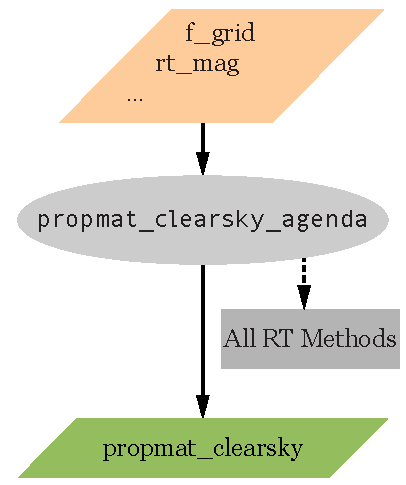
\includegraphics[scale=0.7]{propmat_clearsky_agenda}
  \caption{An outside view of propmat\_clearsky\_agenda.}
  \label{fig:absorption:pmat_outside}
 \end{center}
\end{figure}

The output of the agenda is a single variable,
\wsvindex{propmat\_clearsky}, a tensor with dimensions of absorption
species, frequency, Stokes dimension and Stokes dimension (Stokes
dimension of one thus emulates scalar absorption).  The physical
quantity corresponding to this variable is the clear-sky propagation
matrix \aAbsMat{a}\, as defined in Equation
\ref{eq:propmattotal}. It describes all non-scattering extinction
effects, that is, absorption and related polarization effects.

An inside view of propmat\_clearsky\_agenda is given in Figure
\ref{fig:absorption:pmat_inside}.  The agenda can contain a number of
different workspace methods that in some way or other compute
propmat\_clearsky. See the built-in documentation of the individual
methods to learn more. File \fileindex{agendas.arts}, one of the
standard include-controlfiles, predefines some typical alternatives
how propmat\_clearsky\_agenda can be set for different purposes.

\begin{figure}
 \begin{center}
  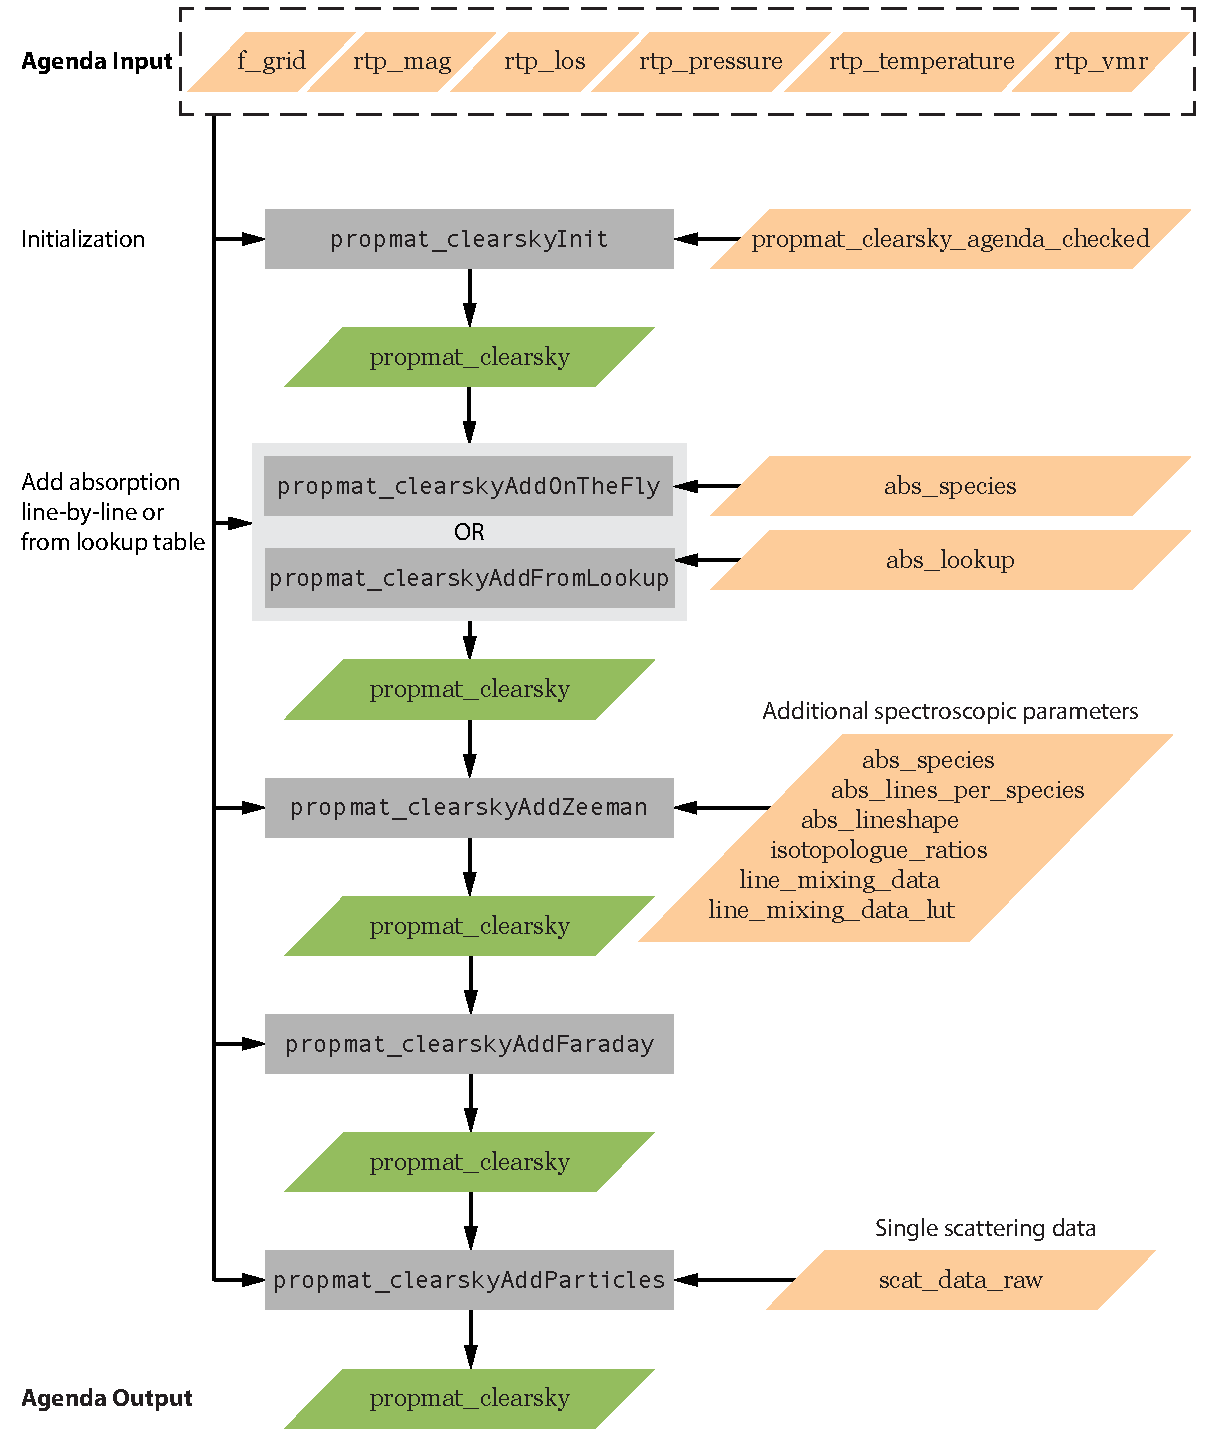
\includegraphics[scale=0.7]{propmat_clearsky_agenda_detail}
  \caption{An inside view of propmat\_clearsky\_agenda. At the same
    time, this gives an outside view of abs\_xsec\_agenda, as input to
    \wsmindex{propmat\_clearskyAddOnTheFly} in the context of
    on-the-fly absorption generation.}
  \label{fig:absorption:pmat_inside}
 \end{center}
\end{figure}



\section{Calculating gas absorption}
\label{sec:absorption:calculating}

This section deals with calculating gas absorption matrices in
ARTS.  This can typically occur in three different contexts:
as on-the-fly absorption matrix calculation within the radiative transfer
calculation,
% (see Section \ref{sec:absorption:abs-rt}), %this reference is more confusing than helping
when preparing
a gas absorption lookup table (see Section \ref{sec:absorption:lookup}),
or when the user is only interested in the absorption itself (see Section
\ref{sec:absorption:abs-only}).

In all these cases, the same agenda is used to actually calculate
absorption: abs\_xsec\_agenda. Outside views of this agenda are shown
in Figure \ref{fig:absorption:pmat_inside} (as input to
\wsmindex{propmat\_clearskyAddOnTheFly} in the context of on-the-fly
absorption generation) and Figure \ref{fig:absorption:xsec_in_lookup}
(as input to \wsmindex{abs\_lookupCalc} in the context of absorption
lookup table generation).

\begin{figure}
 \begin{center}
  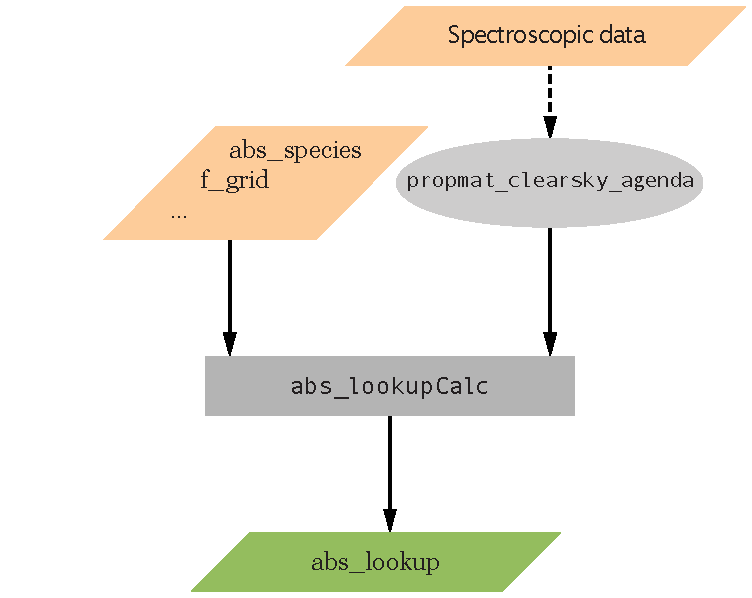
\includegraphics[scale=0.7]{abs_lookupCalc}
  \caption{An outside view of abs\_xsec\_agenda, in the context of
    absorption lookup table generation.}
  \label{fig:absorption:xsec_in_lookup}
 \end{center}
\end{figure}

An inside view of abs\_xsec\_agenda is given in Figure
\ref{fig:absorption:xsec_inside}.  The agenda can contain a number of
different workspace methods that in some way or other compute
abs\_xsec. See the built-in documentation of the individual methods to
learn more. As for propmat\_clearsky\_agenda, file
\fileindex{agendas.arts} predefines some typical alternatives also for
abs\_xsec\_agenda.

\begin{figure}
 \begin{center}
  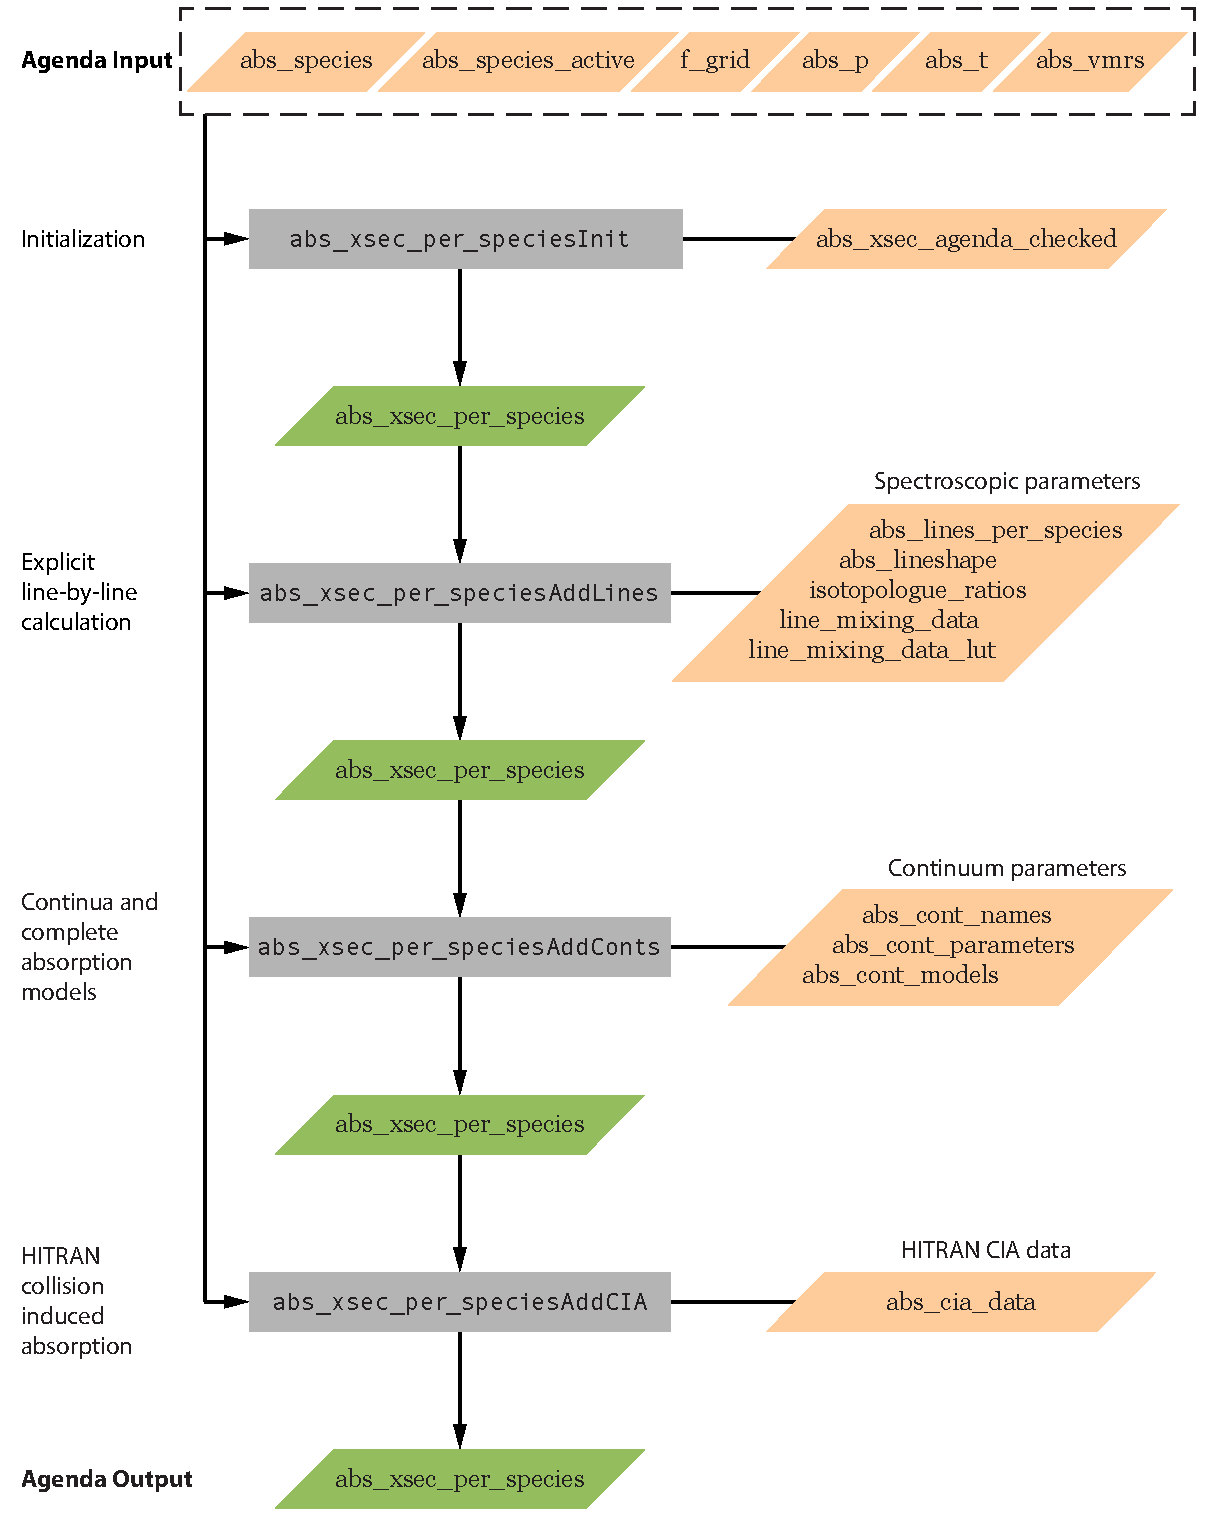
\includegraphics[scale=0.7]{abs_xsec_agenda}
  \caption{An inside view of abs\_xsec\_agenda.}
  \label{fig:absorption:xsec_inside}
 \end{center}
\end{figure}


\subsection{Absorption species}

Absorption is additive, so the total absorption is simply the sum of
all partial absorptions.  And the partial absorption for gases that
have spectral lines can be calculated as a sum over the absorption of
each spectral line, plus some more or less empirical continuum terms.

An absorption species in ARTS is an abstract entity that has a partial
absorption matrix associated with it, and that usually can be
associated with a volume mixing ratio of a corresponding gas (the VMRs
are stored in variable \wsvindex{vmr\_field}). Total absorption is the
sum of the partial absorptions of all absorption species. Absorption
species are defined in the ARTS controlfile by special `tags', which
are stored in the variable \wsvindex{abs\_species}, and set by the
method \wsmindex{abs\_speciesSet}.

The absorption species tags specify the different considered absorbers, which can
be gaseous species but also free electrons and (grey-body) particles.
For gaseous species, they also describe the model that should be used to
calculate the absorption for each of the species.
There are three types of tags, those for explicit line-by-line
calculations, those for continua and complete absorption models, and a special
Zeeman effect tag.
An example of the first kind is \verb|"H2O-18"|, which identifies a
particular isotopologue of water vapor. An example of the second kind is
\verb|"H2O-ForeignContCKDMT100"|, which identifies a particular continuum
model. An example of the third is \verb|"O2-Z"|, which identifies that special Zeeman
routines should be used.
Tags can be combined, if they refer to the same molecule
(different isotopologues are allowed). Even continuum tags can be combined
with explicit line-by-line tags, if they refer to the same molecule.

It should be noted that isotopologue ratios are taken into account
implicitly when line strengths are calculated, so even if you make
calculations for individual isotopologues, the VMR numbers in the
variable \wsvindex{vmr\_field} should not be adjusted for the isotopologue
ratio (the isotopologue ratio can be changed instead; see
Section~\ref{sec:absorption:isoratio}). As an example, to make a line-by-line
calculation for all ozone isotopologues, you could represent them in different
ways by
\wsmindex{abs\_speciesSet}.
\begin{code}
a) abs_speciesSet(species=["O3"])
b) abs_speciesSet(species=
                  ["O3-666, O3-668, O3-686, O3-667, O3-676"])
c) abs_speciesSet(species= 
                  ["O3-666", "O3-668", "O3-686", "O3-667", "O3-676"])
\end{code}
Options (a) and (b) are equivalent, you will have one ozone species
that represents all isotopologues, and that will be associated with a
single VMR field in \wsvindex{vmr\_field}.  With option (c) you have
five different ozone species, so you have to supply five different VMR
fields. If those five fields are identical (exactly same numerical
values), you will get the same total absorption as with options (a)
and (b).

Overall, the tag mechanism allows quite complex absorption setups. The built-in
documentation for \wsmindex{abs\_speciesSet} gives a detailed explanation of the
tag syntax and some examples.

Particularly note, that order of the species list matters as absorption line
data is assigned to species in their order within the \wsvindex{abs\_species}
list and no line record is assigned to more than one species.
It is furthermore important to note that there is no `intelligence' in ARTS that
checks that the chosen tag combinations make sense, so the user should
know what s/he is doing, or follow one of the many examples in
the ARTS \fileindex{controlfiles} directory.

\subsection{Explicit line-by-line calculations}

For absorption species with explicit line-by-line calculation the
calculation involves the steps summarized in Table
\ref{tab:absorption:lbl}, which contains the steps that are common to all the
three contexts in which explicit line-by-line calculations can occur as well
as the steps that are specific to each of those cases. 
The list of variables and methods in the
table is not complete. The idea is to give an overview over the
important ones and show how they work together. Missing are
particularly the input variables that describe the atmospheric
conditions, and continuum description variables, which normally do not
have to be set by the user anyway.

\begin{table}
\footnotesize
\renewcommand{\arraystretch}{1.5}
\newcounter{rownum}
\newcommand{\mylabel}[1]{\refstepcounter{rownum} \label{#1}}
\begin{tabularx}{\hsize}{l>{\raggedright\arraybackslash\hsize=0.5\hsize}X
                          >{\raggedright\arraybackslash\hsize=1.5\hsize}X}
\hline
\# & Step & Variables and Methods \\
\hline
%---------------------------------------------------------------------
\mylabel{step:lineshape}
\arabic{rownum} & 
Define line shape function(s) to use. &
Variable:
\wsvindex{abs\_lineshape}. \newline
Methods:
\wsmindex{abs\_lineshapeDefine} (same shape for all species),
\wsmindex{abs\_lineshape\_per\_tgDefine} (different shapes for different
species). \\
%---------------------------------------------------------------------
\mylabel{step:readline}
\arabic{rownum} &
Read spectral line data (the order of the first two steps does not
matter). &
Variable: \wsvindex{abs\_lines}. \newline
Methods: 
\wsmindex{abs\_linesReadFromArts},
\wsmindex{abs\_linesReadFromSplitArtscat},
\wsmindex{abs\_linesReadFromHitran},
\wsmindex{abs\_linesReadFromHitranPre2004},
\wsmindex{abs\_linesReadFromJpl},
\wsmindex{abs\_linesReadFromMytran2} (different methods are for
different catalogue formats). For the ARTS internal format, the
standard method \wsmindex{ReadXML} works also, but does not allow to
select a frequency range, as the others do. \\
%---------------------------------------------------------------------
\mylabel{step:splitline}
\arabic{rownum} &
Split line data for different absorption species. &
Variable: \wsvindex{abs\_lines\_per\_species}. \newline
Methods:
\wsmindex{abs\_lines\_per\_speciesCreateFromLines}. Alternatively, read
lines from different catalogues for different species directly with
\wsmindex{abs\_lines\_per\_speciesReadFromCatalogues}. \\
%---------------------------------------------------------------------
\mylabel{step:optline}
\arabic{rownum} &
Optimize line data. (optional)&
Variable: \wsvindex{abs\_lines\_per\_species}. \newline
Methods: Add mirror lines for VVW line shape with
\wsmindex{abs\_lines\_per\_speciesAddMirrorLines} (see \theory,
Chapter \ref{T-sec:abs_theory}). Remove lines that are outside the
line shape cutoff with \wsmindex{abs\_lines\_per\_speciesCompact}. \\
%---------------------------------------------------------------------
\multicolumn{3}{>{\raggedright\arraybackslash\hsize=2\hsize}X}{The
  first four steps are preparation, and typically 
  have to be done only once per ARTS run. The fifth step is the actual
  absorption calculation, which can occur in different contexts.} \\
%---------------------------------------------------------------------
\mylabel{step:calc}
\arabic{rownum}a &
Calculate absorption on-the-fly. &
Agenda: \wsaindex{propmat\_clearsky\_agenda}. \newline
Variable: \wsvindex{propmat\_clearsky}, which is nitialized in \wsmindex{propmat\_clearskyInit}.\newline
Methods: \wsmindex{propmat\_clearskyAddOnTheFly} (the core method for on-the-fly
absoprtion calculation inlcuding line-by-line and continuum absorption), \newline
\wsmindex{propmat\_clearskyAddZeeman} (see Sec.~\ref{sec:absorption:zeeman}), \newline
\wsmindex{propmat\_clearskyAddFaraday} (see Sec.~\ref{sec:absorption:faraday}), \newline
\wsmindex{propmat\_clearskyAddParticles} (see Sec.~\ref{sec:absorption:particles}). \newline
Alternative:
\wsmindex{propmat\_clearskyAddFromLookup} instead of \wsmindex{propmat\_clearskyAddOnTheFly}
(extract absorption from pre-calculated lookup table, see
Sec.~\ref{sec:absorption:lookup}). Note that the lookup
table cannot contain absorption for Zeeman tagged species, Faraday rotation, and
particles due to their directional dependencies.\\
%---------------------------------------------------------------------
\arabic{rownum}b &
Calculate absorption lookup table. &
Variable: \wsvindex{abs\_lookup}. \newline
Methods: \wsmindex{abs\_lookupCalc}. Alternative: Load lookup table
from file with \wsmindex{ReadXML}, it then has to be adapted to the
current calculation (and checked) with \wsmindex{abs\_lookupAdapt}. \\ 
%---------------------------------------------------------------------
\arabic{rownum}c &
Calculate absorption only (no RT). &
Variable: \wsvindex{propmat\_clearsky\_field}, \wsvindex{abs\_coef}. \newline
Methods, high level: \wsmindex{propmat\_clearsky\_fieldCalc}. \newline
Methods, low level: \newline
\wsmindex{abs\_xsec\_per\_speciesInit}, \newline
\wsmindex{abs\_xsec\_per\_speciesAddLines} (the core method for the
actual line-by-line calculation, used internally by all higher level methods),\newline
\wsmindex{abs\_xsec\_per\_speciesAddConts} (add continua or complete absorption
models, see Section \ref{sec:absorption:continua}),\newline
\wsmindex{abs\_xsec\_per\_speciesAddCIA} (add collision induced absorption, see
Section \ref{sec:absorption:cia}),\newline
\wsmindex{abs\_coefCalcFromXsec} (calculate absorption coefficients
from absorption cross-sections). \\
%---------------------------------------------------------------------
\hline
\end{tabularx}
\caption{Steps for line-by-line absorption calculation, and associated
    ARTS workspace variables and methods.}
\label{tab:absorption:lbl}
\end{table}

See the built-in documentation of the various variables and methods
for more information.  It is on purpose not repeated here, for better
maintainability.  If you are viewing this pdf file on a computer, just
click on a variable or method name to get to the corresponding
built-in documentation. Further input data and parameters required (not only)
for line-by-line calculations is described in Section~\ref{sec:absorption:input}.

\subsection{Continua and complete absorption models}
\label{sec:absorption:continua}

ARTS includes many absorption continua and complete absorption models,
which are described in \theory, Chapter \ref{T-sec:abs_theory}.  The
common property of all of these is that they do not use the standard
ARTS line-by-line calculation mechanism.  They may include spectral
lines, but then these lines are hardwired into the absorption model
itself.  Consequently, the first four steps in Table
\ref{tab:absorption:lbl} are not needed for these models.  

The pure continua are intended to be used together with an explicit ARTS
line-by-line calculation, the complete models are intended to be used alone.
To select a continuum or complete absorption model, simply use the
corresponding tag with \wsmindex{abs\_speciesSet}.  Currently available
models are listed in Table \ref{tab:absorption:continua}.

\begin{table}
\centering
\footnotesize
\begin{tabular}{ll}
\hline  
Class & Tag name \\
\hline  
%---------------------------------------------------------------------

Water vapor continua
& H2O-SelfContStandardType \\
& H2O-ForeignContStandardType \\
& H2O-ForeignContMaTippingType \\
& H2O-ContMPM93 \\
& H2O-SelfContCKD222 \\
& H2O-ForeignContCKD222 \\
& H2O-SelfContCKD242 \\
& H2O-ForeignContCKD242 \\
& H2O-SelfContCKD24 \\
& H2O-ForeignContCKD24 \\
& H2O-SelfContCKDMT100 \\
& H2O-ForeignContCKDMT100 \\
& H2O-SelfContCKDMT252 \\
& H2O-ForeignContCKDMT252 \\
& H2O-ForeignContATM01 \\[1ex]

Complete water vapor models
& H2O-CP98 \\
& H2O-MPM87 \\
& H2O-MPM89 \\
& H2O-MPM93 \\
& H2O-PWR98 \\[1ex]

Carbon dioxide continua 
& CO2-CKD241 \\
& CO2-CKDMT100 \\
& CO2-CKDMT252 \\
& CO2-SelfContPWR93 \\
& CO2-ForeignContPWR93 \\
& CO2-SelfContHo66 \\
& CO2-ForeignContHo66 \\[1ex]

Oxygen continua 
& O2-CIAfunCKDMT100 \\
& O2-v0v0CKDMT100 \\
& O2-v1v0CKDMT100 \\
& O2-visCKDMT252 \\
& O2-SelfContStandardType \\
& O2-SelfContMPM93 \\
& O2-SelfContPWR93 \\[1ex]

Complete oxygen models & O2-PWR98 \\
& O2-PWR93 \\
& O2-PWR88 \\
& O2-MPM93 \\
& O2-MPM92 \\
& O2-MPM89 \\
& O2-MPM87 \\
& O2-MPM85 \\
& O2-TRE05 \\[1ex]

Nitrogen continua & N2-SelfContMPM93 \\
& N2-SelfContPWR93 \\
& N2-SelfContStandardType \\
& N2-SelfContBorysow \\
& N2-CIArotCKDMT100 \\
& N2-CIAfunCKDMT100 \\
& N2-CIArotCKDMT252 \\
& N2-CIAfunCKDMT252 \\
& N2-DryContATM01 \\[1ex]

Condensate absorption models & liquidcloud-MPM93 \\
& icecloud-MPM93 \\
& rain-MPM93 \\

%---------------------------------------------------------------------
\hline  
\end{tabular}
\caption{ARTS continua and complete absorption models. The molecular
  species can be inferred from the start of the tag name.  See
  \theory, Chapter \ref{T-sec:abs_theory} for more information on the
  various models.}
\label{tab:absorption:continua}
\end{table}

The names should be fairly self-explanatory and can be used to find
background information on the various models in \theory.  The
condensate absorption models are a bit special and perhaps need some
extra explanation. They are absorption parameterizations by Liebe, and
allow the inclusion of condensate in the (rare) cases where scattering
is not important. Their general applicability is therefore fairly limited.

The behavior of the continua and complete absorption models can be
modified by passing them some additional parameters, stored in the
variables \wsvindex{abs\_cont\_names}, \wsvindex{abs\_cont\_models},
and \wsvindex{abs\_cont\_parameters}. Basically,
\builtindoc{abs\_cont\_names} identifies the model,
\builtindoc{abs\_cont\_models} contains switches that select different
behavior (for example taking only the lines, or only the continuum
part of a complete model), and \builtindoc{abs\_cont\_parameters} can
contain numerical parameters. 

Yes, the nomenclature for these additional continuum parameters,
particularly \builtindoc{abs\_cont\_models}, is confusing. However,
most users will never have to deal with these variables
explicitly. They are set to default values in the include file
\fileindex{continua.arts}. Users should therefore always include this file  at
the start of their controlfiles with
\begin{code}
  INCLUDE "continua.arts"
\end{code}
Unless you work on continuum model development or verification, you
should never have to modify these default settings.

The core method to calculate continua and complete absorption models
is \wsmindex{abs\_xsec\_per\_speciesAddConts}.  Users normally do not
have to call this method explicitly, since it is used implicitly by
higher level methods, such as \wsmindex{propmat\_clearskyAddOnTheFly} and
\wsmindex{propmat\_clearsky\_fieldCalc}.

\subsection{Collision-induced absorption}
\label{sec:absorption:cia}

Collisions of centro-symmetric molecules, e.g., \chem{O_2},
\chem{N_2}, \chem{H_2}, \chem{CO_2}, and \chem{CH_4}, possessing no permanent
electric dipole create a transient dipole, which causes so-called collision-induced
absorption (CIA). Absorption strength of CIA is characterized by its dependency
on the molecular density of both molecular species involved in the collision.

Recently, the well-known HITRAN spectral line catalogue has started to
offer also tabulated binary absorption cross-sections for CIA.  This is
described in detail in \citet{richard:12}, and also in the documentation that
comes with the data themselves.

Binary absorption cross-sections
\aAbsXsec{i,j} have to be multiplied with the number densities of both involved
molecular species to yield absorption coefficients:
\begin{equation}
\aAbsCoef{i,j} =  \aAbsXsec{i,j} \, \aDen{i} \, \aDen{j},
\end{equation}
where $i$ and $j$ denote the two different absorbing species. As a
consequence, \aAbsXsec{i,j} has units of m$^5$/molec$^2$ in ARTS (the
original HITRAN units are different).

Using CIA in ARTS is easy. First of all, include one or more CIA tags
in your absorption species list (\wsvindex{abs\_species}). All valid
tags are listed in Table \ref{tab:absorption:cia_ranges}. Secondly,
read in WSV \wsvindex{abs\_cia\_data}, which contains the tabulated
binary absorption cross-sections, from a file. This will usually be the
file \fileindex{hitran\_cia2012\_adapted.xml.gz}, which is included in the
\shortcode{arts-xml-data}, but the original HITRAN data files can also be
read. Finally, use WSM \wsmindex{abs\_xsec\_per\_speciesAddCIA} in
abs\_xsec\_agenda to add the CIA absorption. For usage examples, look
in directory \fileindex{controlfiles/artscomponents/cia} that is part
of the ARTS distribution.

Figure \ref{fig:absorption:cia} shows all CIA continua that are
currently available in ARTS (left) and separately the ones that are
relevant for Earth's atmosphere (right). The valid frequency and
temperature ranges for these data, as available in ARTS, are listed in
Table \ref{tab:absorption:cia_ranges}. Outside the covered frequency ranges, the
binary absorption cross-sections are set to zero, while exceeding the valid
temperature range will produce \verb|NaN| values and eventually trigger a
runtime error.

To make the HITRAN data work in ARTS, some modifications were necessary,
specifically:

\begin{description}
\item[N$_2$-N$_2$:] The two high-frequency datasets were merged into one.
\item[O$_2$-O$_2$:] Three apparently separate datasets that really
  belong together were merged. UV/Vis dataset were removed.
\item[CO$_2$-CO$_2$:] Caveat: This is only the self continuum of
  CO2. The CO2-air continuum has strong features above 250\,cm$^{-1}$ that
  are present in CKD\_MT (also available in ARTS as one of the
  continuum and full absorption models), but are missing here.
  %The HITRAN data also generally looks weird. It is only in the alternative
  %folder, and \citet{richard:12} basically recommend not to use it. Conclusion:
  %No changes, but usage not recommended.
  Furthermore, \citet{richard:12} point out that for molecules with more than two atoms
  further mechanisms affecting CIA exist, which are not covered by the simple
  models used. They hence state that ``these data should be used very
  carefully''. Conclusion: No changes, but use with care.

  Also note that no data exists at frequencies below 30\,GHz (1\,cm$^{-1}$)
  though some significant absorption is still present at the limiting frequency.
  For those low frequencies, the CO2-SelfContPWR93 continuum (see
  Table~\ref{tab:absorption:continua}) can be used as an alternative (we
  estimated that to be valid at least up to about 100\,GHz, but deviating
  significantly above 500\,GHz).
\item[O2-N2, O2-CO2:] These UV/Vis-only datasets were removed.

\begin{table}
    \caption{Absorption species tags, frequency ranges, and
      temperature ranges for HITRAN CIA data as implemented in
      ARTS. (These data contain some modifications from the original
      HITRAN data, which are described in the text.)} 
    \label{tab:absorption:cia_ranges}
    \centering
    \begin{tabular}{llll}
\hline
    CIA tag& Spectral range [cm$^{-1}$]& Temp range [K]& No. of datasets\\
\hline
  N2-CIA-N2-0& 0.02 -- 554.00& 40.00 -- 400.00& 10\\
  N2-CIA-N2-1& 1850.00 -- 3000.09& 228.20 -- 362.50& 10\\
  N2-CIA-H2-0& 0.02 -- 1886.00& 40.00 -- 400.00& 10\\
  N2-CIA-CH4-0& 0.02 -- 1379.00& 40.00 -- 400.00& 10\\
  H2-CIA-H2-0& 20.00 -- 10000.00& 200.00 -- 3000.00& 113\\
  H2-CIA-He-0& 20.00 -- 20000.00& 200.00 -- 9900.00& 334\\
  H2-CIA-CH4-0& 0.02 -- 1946.00& 40.00 -- 400.00& 10\\
  H2-CIA-H-0& 100.00 -- 10000.00& 1000.00 -- 2500.00& 4\\
  He-CIA-H-0& 50.00 -- 11000.00& 1500.00 -- 10000.00& 10\\
  O2-CIA-O2-0& 1150.00 -- 1950.00& 193.40 -- 353.40& 15\\
  CO2-CIA-CO2-0& 1.00 -- 250.00& 200.00 -- 800.00& 7\\
  CH4-CIA-CH4-0& 0.02 -- 990.00& 40.00 -- 400.00& 10\\
  CH4-CIA-Ar-0& 1.00 -- 697.00& 70.00 -- 296.00& 5\\
\hline
\end{tabular}
\end{table}


\end{description}

\begin{figure}
 \begin{center}
  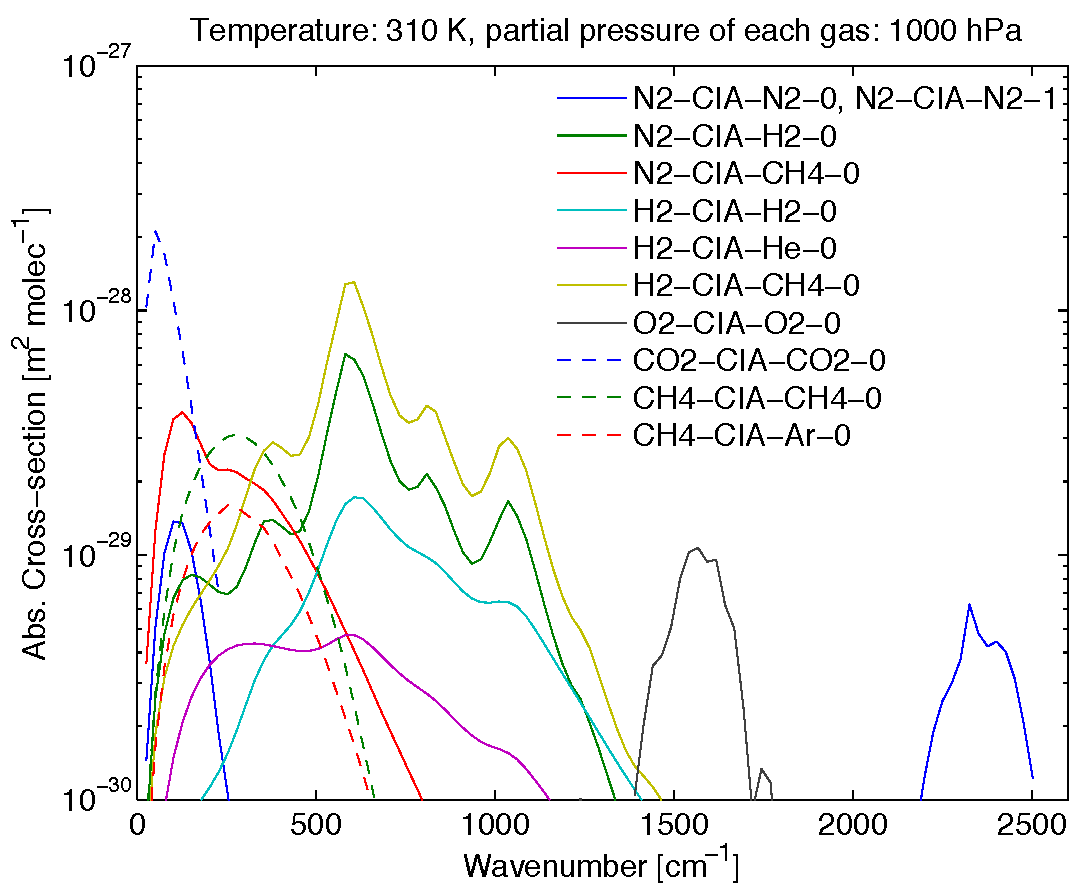
\includegraphics[width=.46\hsize]{plot_all_arts_cia_generic_1}
  \hspace{\fill}
  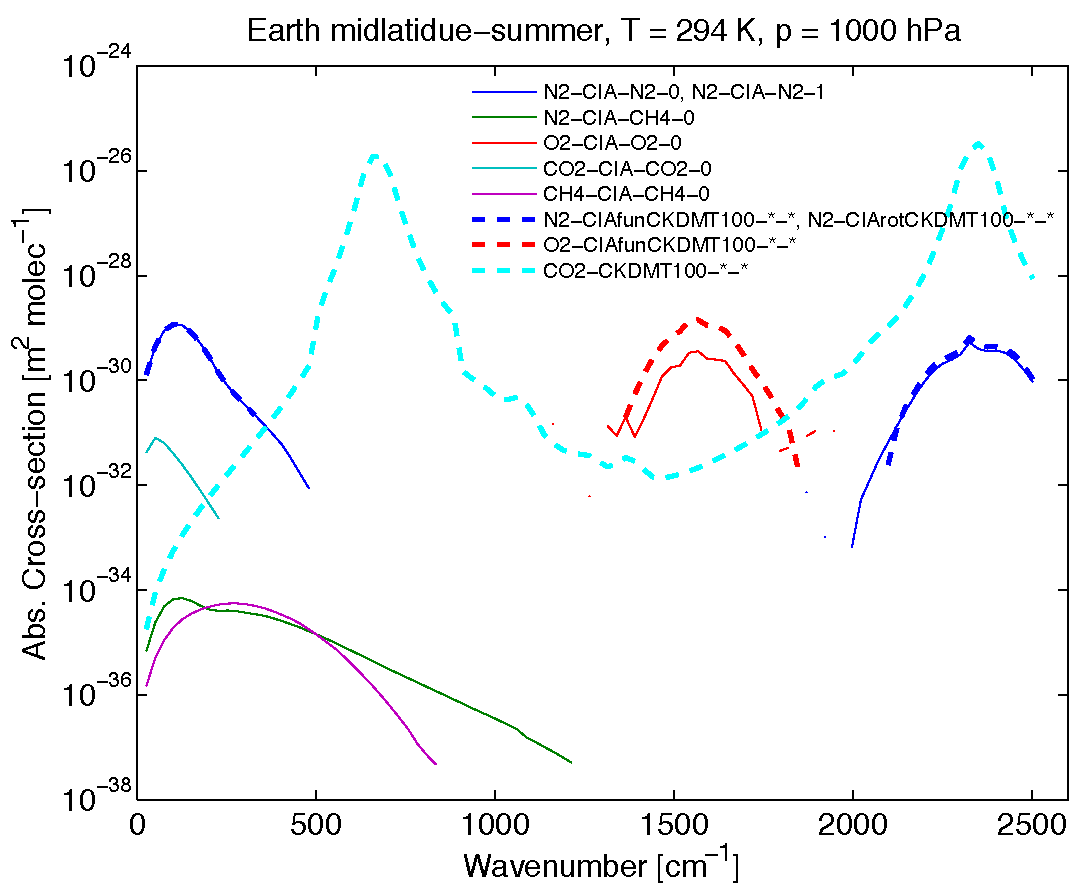
\includegraphics[width=.46\hsize]{plot_earth_continua_1_1}
  \caption{Left: All HITRAN CIA continua that are implemented in ARTS
    (each gas here has a partial pressure of 1000\,hPa). Right: Only
    the ones that are relevant for Earth (for Earth surface
    conditions).}
  \label{fig:absorption:cia}
 \end{center}
\end{figure}

\subsection{Zeeman calculations}
\label{sec:absorption:zeeman}

The Zeeman effect is calculated in the method \wsmindex{propmat\_clearskyAddZeeman}.
If this method is included in the \builtindoc{propmat\_clearsky\_agenda}, then species with the
tag "\verb|-Z|" will be calculated as Zeeman species. If the method is not included,
then these species will simply be ignored. Note that the order within the tag
string is important: the Zeeman tag must directly follow the molecular species
tag. That is, \verb|O2-Z-66| will be counted as Zeeman splitting on the
O$^{16}$O$^{16}$ molecule, whereas \verb|O2-66-Z| will not work the same way, or even at all.

The physics and internal workings of the Zeeman calculations follow the scheme
presented in \citet{larsson:xx} %FIXME: update bibtex reference when accepted.
%Larsson et al., submitted 2013 to JQSRT, \textit{A treatment of the Zeeman
%effect using Stokes formalism and its implementation in the Atmospheric
%Radiative Transfer Simulator ARTS}.

In order to calculate Zeeman splitting, additional line parameters that are not
readily available in, e.g., HITRAN are necessary. These include $g_s$ [-], the
relative Land\'{e} factor, and $S$ [-], the molecular total spin. These
variables must therefore be read to the WSV \wsvindex{isotopologue\_quantum}.
This variable is of type \builtindoc{SpeciesAuxData}, and a file providing
that kind of data would, e.g., look like:
\begin{code}
<arts format="ascii" version="1">
  <SpeciesAuxData version="1" nelem="1" nparam="3">
    @ O2-66 2.002064 1 1
  </SpeciesAuxData>
</arts>
\end{code}
In this example, \verb|@| indicates the beginning of a new data record, \verb|O2-66|
specifies what isotopologue is associated with the data, the number
\verb|2.002064| is the relative Land\'{e} factor, and the molecule got $S=1$.
The last value indicates what Hund case is used in the calculations. For oxygen,
Hund case b is used, indicated b the number "1". Presently, Hund case a, indicated
by number "0" also works for some molecules. It is up to the user to assure the
correct quantum numbers for each case are set properly.
The supported molecules in ARTS so far for Zeeman calculations are
\begin{itemize}
\item O$_2$, case b
\item NO, case a/b
\item OH, case a
\item ClO, case a
\item HO$_2$, case b
\item NO$_2$, case b
\end{itemize}
but only O$_2$ is tested beyond initial modeling results.

Beside the additional line parameters, it is also necessary to input the magnetic
field into the model. This can be done following:
\begin{code}
GriddedField3Create(B)
  ReadXML(B,"B_1comp.xml.gz")
  GriddedFieldLatLonRegrid( B, lat_grid, lon_grid, B )
  GriddedFieldPRegrid( B, p_grid, B )
  FieldFromGriddedField( mag_w_field, p_grid, lat_grid, 
                         lon_grid, B )
\end{code}
where \verb|B_1comp.xml.gz| contains the (atmospheric) profile or field for one
components of the magnetic field. 
Since the magnetic field is usually not dependent on the pressure,
it is also possible to use the  
\begin{code}
 GriddedFieldZToPRegrid(*)
\end{code}
functionality to input altitude-gridded magnetism.
Input needs to be provided for each non-zero
magnetic field component separately into the respective WSVs \wsvindex{mag\_w\_field}, 
\wsvindex{mag\_v\_field}, and \wsvindex{mag\_u\_field}. For more information on
magnetic field format in ARTS see Section~\ref{sec:atm:vecfields}.

Lastly, it is necessary to take phase effects into account when calculating the
Zeeman effect. It is therefore important that \wsvindex{abs\_lineshape} is
chosen such that it allows for this information to be provided. One
suitable line shape can be defined through
\begin{code}
abs_lineshapeDefine( abs_lineshape, "Faddeeva_Algorithm_916", 
                     "VVH", 750e9 )
\end{code}

\subsection{Internal line-mixing}
\label{sec:absorption:line-mixing}

Line mixing is implemented as the \verb|-LM-| species tag.  Added to 
a species, ARTS knows that it should look for lines with
line mixing data attached to them when it calculates the spectral cross sections.
Note that each line is initialized without any line mixing data, and with a tag 
state that says they are not to be line mixed.  If this is not changed before the
absorption calculations are performed, the line will regardless of species tag still
act like if it were not line mixed.  Also note that it is possible to calculate line mixing
in conjuncture with the Zeeman effect, but that it is not possible to calculate the line mixing
of individual Zeeman lines, which as far as we know when writing this is unimportant.

The possible tags on species \verb|X| that activates the line mixing module are thus
\verb|X-LM-*|, and \verb|X-Z-LM-*|.
The supported ways to ensure that the line record contains information on
how to calculate line mixing, thus not ignoring it, are 
\begin{itemize}
 \item Read an ARTS catalogue file with line mixing parameters.
 \item Read LBLRTM line catalogue containing line mixing parameters using 
 \verb|abs_linesReadFromLBLRTM(*)|.
 \item Read a line database that does not have line mixing, but use the 
 \verb|line_mixing_dataMatch(*)| method to inject line mixing data into the line record.
\end{itemize}
There is no preferred method in ARTS --- each work the same when they reach the absorption
calculations --- but we urge the user to be sure that line mixing data and the line database
are of the same origin, as the calculations will be of poor quality if this is not the case.

Example control file meta flow for code calculating line mixing using \verb|abs_linesReadFromLBLRTM|:
\begin{code}
# Define your atmospheric species,
abs_speciesSet(species=["O2-Z-LM","CO2-LM"])

# read from a line database,
abs_linesReadFromLBLRTM(filename="aer", 
    fmin=1e1,fmax=1e20)
\end{code}
Note that this meta flow is very similar to using an ARTS catalogue with line mixing.
These methods are easy, because they identity what line mixing method will be used 
directly from the catalogue.
It should be noted that LBLRTM also gives the non-resonant term of the molecular oxygen
spectra as a low frequency line.  If it is desired to calculate this term, the lower
frequency range must contain the line as per the definition of our reading routines.

Example control file meta flow for code calculating line mixing using \verb|line_mixing_dataMatch|:
\begin{code}
# Define your atmospheric species,
abs_speciesSet(species=["O2-Z-LM","CO2-LM"])

# Read from a line database,
abs_linesReadFromHITRAN(filename="HITRAN2012.par", 
    fmin=1e1,fmax=1e20)

# Sort the line records into the format ARTS wants
abs_lines_per_speciesCreateFromLines

# Create a way to temporally store O2 line mixing data.
ArrayOfLineMixingRecordCreate(lm_o2)
ReadXML(lm_o2,"o2.xml")

# Create a way to temporally store CO2 line mixing data.
ArrayOfLineMixingRecordCreate(lm_co2)
ReadXML(lm_co2,"co2.xml")

# Match the line mixing data with O2 and Zeeman effect
line_mixing_dataMatch(
    species_tag="O2-Z-LM",
    line_mixing_records=lm_o2
    line_mixing_tag=LM*)

# Match the line mixing data with O2 and Zeeman effect
line_mixing_dataMatch(
    species_tag="CO2-LM",
    line_mixing_records=lm_co2,
    line_mixing_tag=LM*)
\end{code}
The latter method is much more complicated than reading directly from the catalogue.
This is because the user has to ensure what type of line mixing is going on
and then parse that data properly to ARTS.  In order for ARTS to know what line the user 
wants to line mix, a series of line database matching 
based on the quantum numbers of the line is necessary.
This means that it only works for those species and catalogue formats
for which we have implemented quantum number reading.
This list is small but growing, and if you need help adding another species, 
let us know via the mailing list.

There are three \verb|line_mixing_tag| supported at this point:
\verb|"LL"|, \verb|"NR"| and \verb|"L2"|.  These refer to LBLRTM, and second order line mixing.
Setting these tags will tell ARTS how to calculate the line mixing of any particular line.
The data is matched from \verb|ArrayOfLineMixingRecord|,
which must contain a \verb|SpeciesTag|, a
\verb|QuantumNumberRecord|, and a vector that is the correct length for the method selected

Example of correct input data for using the second order approach ("L2"):
\begin{code}
<?xml version="1.0"?>
<arts format="ascii" version="1">
<Array type="LineMixingRecord" nelem="38">
<LineMixingRecord>
<SpeciesTag>"O2-66-*-*"</SpeciesTag>
<QuantumNumberRecord>
<Upper><QuantumNumbers nelem="3"> 
  J 1/1 N 1/1 v1 0/1 
</QuantumNumbers></Upper>
<Lower><QuantumNumbers nelem="3"> 
  J 2/1 N 1/1 v1 0/1 
</QuantumNumbers></Lower>
</QuantumNumberRecord>
<Vector nelem="10">
2.65e-06
-1.32e-07
-8.35e-12
8.43e-13
0.000545
0.00017
300
0.8
1.6
1.6
</Vector>
</LineMixingRecord>
</Array>
</arts>
\end{code}
The format of the above data is thusly: \shortcode{SpeciesTag},
\shortcode{QuantumNumberRecord}, \shortcode{Vector}, 
The above input will cause the \verb|O2-66-*-*| line with
upper quantum numbers $J=1$, $N=1$ and $\nu_1=0$ and with
lower quantum numbers $J=2$, $N=1$ and $\nu_1=0$ to match.
If this is the only input file, the described line is the only
line experiencing line mixing in your calculations. If there
were more lines in the file, these would also experience line mixing.
In order of appearance in the vector, its format is 
first order zeroth phase correction [Pa$^{-1}$], 
first order first phase correction [Pa$^{-1}$],
second order zeroth absorption correction [Pa$^{-2}$],
second order first absorption correction [Pa$^{-2}$],
second order zeroth line-center correction [Hz Pa$^{-2}$],
second order first line-center correction [Hz Pa$^{-2}$],
standard temperature for corrections [K],
first order phase temperature correction exponential term [-],
second order absorption temperature correction exponential term [-], and
second order line-center temperature correction exponential term [-].
The format of the vector is fixed according to necessary information found 
in \citet{makarov11:_60-ghz_jqsrt},
the naming scheme of the variables above can also be understood from the same work.
Note that first order line mixing, as per the MPM/PWR complete oxygen models, 
can be achieved with the correct input by letting the second order terms be nil.



Example of correct input data for using the LBLRTM approach ("LL" and "NR"):
\begin{code}
<?xml version="1.0"?>
<arts format="ascii" version="1">
<Array type="LineMixingRecord" nelem="38">
<LineMixingRecord>
<SpeciesTag>"O2-66-*-*"</SpeciesTag>
<QuantumNumberRecord>
<Upper><QuantumNumbers nelem="3"> 
  J 1/1 N 1/1 v1 0/1 
</QuantumNumbers></Upper>
<Lower><QuantumNumbers nelem="3"> 
  J 2/1 N 1/1 v1 0/1 
</QuantumNumbers></Lower>
</QuantumNumberRecord>
<Vector nelem="12">
200
250
296
340
-0.004433034295584e-4
-0.003982500863558e-4
-0.003628075993092e-4
-0.003341074759437e-4
0
0
0
0
</Vector>
</LineMixingRecord>
</Array>
</arts>
\end{code}
In this format, the first four values are a temperature grid in Kelvin.
For "LL" the following four values are the first order
line mixing coefficients at these temperature grid points [in units 1/Pa], 
and the last four are the second order line mixing coefficients at these temperature grid points [in units 1/Pa$^2$].
For "NR" the following four values are the first order
non-resonant term at these temperature grid points [in units 1/Pa], 
and the last four are the second order non-resonant terms
at these temperature grid points [in units 1/Pa$^2$].
ARTS will use linear interpolation to get proper coefficients between and slightly outside grid points.

\textit{Warning:} There appears to be some errors in the quantum number encoding
in HITRAN04 and HITRAN08 that makes the line mixing module wrong.  The newer
HITRAN2012 has fixed these issues.

\subsection{Faraday rotation}
\label{sec:absorption:faraday}

Faraday rotation is a change of polarization state of radiation in interaction
with (free) electrons in presence of a static magnatic field. For further
details on theory and usage in ARTS see Section~\ref{sec:faraday}.
Here we only give a short summary how to setup the calculation of Faraday
contribution to the absorption (or better: propagation) matrix
\wsvindex{propmat\_clearsky}.

First, to include Faraday rotation effects
\wsmindex{propmat\_clearskyAddFaraday} must be included in the
\builtindoc{propmat\_clearsky\_agenda}. Second, a species tag
\verb|"free_electrons"| needs to be contained in \wsvindex{abs\_species}.
Correspondingly, a field of electron densities is required in
\builtindoc{vmr\_field}.

For usage examples, check \fileindex{controlfiles/artscomponents/faraday} that
is part of the ARTS distribution.

\subsection{Absorbing particles}
\label{sec:absorption:particles}

% what are particles doing here? what for / when is this useful?
As pointed out before, this chapter deals with absorption by non-scattering
matter. In first place this refers to gases, while particles (aerosols, clouds,
precipitation) are considered to (also) scatter radiation and are handled
differently (see Chapters~\ref{sec:clouds}, \ref{sec:scattering:doit}, and
\ref{sec:scattering:mc}).
However, when particles are small compared to the wavelength of the radiation
they act as broadband grey-body absorbers and can be treated similarly to
continuum absorption by gases.

This is reflected in ARTS providing a few continuum models for condensed
matter (see Tab.~\ref{tab:absorption:continua}), which essentially are
particles, too.
It is tedious, though, to implement those kind of particle continua for a wide
range of different base materials as become of interest when being interested in
other than the Earth's atmosphere.

% concept (using scat_data/pnd_field-type data exists - make use of that)
In the ARTS scattering modules, particles are represented by single scattering
property data (\builtindoc{scat\_data}) and particle concentrations
(particle number densitity fields \builtindoc{pnd\_field}).
% These data usually originate from scattering theory (e.g., Mie theory,
% T-matrix model, Discrete dipole approximation) convolved with size
% distribution models and veetical and horizontal concentration distribution
% information.
The single scattering data originate from scattering theory
programs (e.g., Mie theory, T-matrix model, Discrete Dipole Approximation) and
their preparation typically requires significant efforts. Comprehensive data for
hydrometeors in the Earth atmosphere, but also clouds, dust and the like for
other planets is available from the \shortcode{arts-xml-data} package.
It is appealing to apply this data in non-scattering calculations (e.g. at low
frequencies, where the scattering contribution is negligible) in a consistent
manner. The ARTS method for that is \wsmindex{propmat\_clearskyAddParticles} and
its application is described in the following.

% how to setup
% - per particle type one "particle" tag in abs_species
% - corresponding pnd field into vmr_field
% - one entry per particle type into scat_data_single
% - (directional dependent absorption, polarized absoprtion)
To consider grey-body particle absorption, the user has to include
\wsmindex{propmat\_clearskyAddParticles} in the
\builtindoc{propmat\_clearsky\_agenda}. Furthermore, for each scattering element
(see Section~\ref{sec:clouds:intro} for how a scattering element is defined) 1) a
\verb|"particles"| tag needs to be added to \builtindoc{abs\_species}, 2) the
corresponding concentration field has to be added to \builtindoc{vmr\_field},
and 3) its single scattering data have to be added to
\wsvindex{scat\_data}. This can be done each-by-each using
\builtindoc{ReadXML} and \builtindoc{Append} methods, but a dedicated method
\wsmindex{ScatElementsToabs\_speciesAdd} is available performing these three
steps for one scattering element at once. \wsmindex{ScatElementsToabs\_speciesAdd}
adds the raw number density field to \builtindoc{vmr\_field\_raw}, i.e., the raw
concentration fields can be converted to internal atmospheric grids together
with the gas concentration fields using, e.g., \builtindoc{AtmFieldsCalc}.
Single scattering data of all individual scattering elements is added to one and
the same scattering species, specifically to the last one of these in the
\builtindoc{scat\_data} array.
Note that \wsmindex{ScatElementsToabs\_speciesAdd} is essentially doing the same
as \builtindoc{ScatElementsPndAndScatAdd}, but for non-scattering instead for
scattering-in-cloudbox cases (where in non-scattering setups the concentration
data is stored together with gas concentrations in \builtindoc{vmr\_field},
while for scattering setups it is stored separately in
\builtindoc{pnd\_field}), and that for the single scattering data and
concentration fields the exact same data can be applied.

% caveats: not to be used together with cloudbox - it's either or.
% plus/pro: in contrast to particles as continuum model, it consiers direction
% dependent and polarized absorption as occuring e.g. for non-spherical particles.
Beside being able to re-use particle data from scattering cases, this method is
also advantageous compared to the particles-as-continuum-models implementations
as it allows for directional dependent absorption and for polarization effects
that occur, e.g., with non-spherical particles.

In the default case, absorption by particles is applied both in the extinction
and emission terms of the radiative transfer equation, i.e. both right hand
terms in Equation~\ref{eq:VRTE1}. However, using a flag,
\wsmindex{propmat\_clearskyAddParticles} can apply total particle extinction
instead. It shall be noted, that while this applies the correct extinction, it
also creates an unphysical emission term. Hence, this option shall only be
applied when the source term is negligible, as e.g. for occultation
measurements.

Be aware that both \wsmindex{propmat\_clearskyAddParticles} and the scattering methods
use \wsvindex{scat\_data} to store the particle single scattering data.
Hence, it is straight-forward that these methods can not be applied
simultaneously. In one ARTS run, all particles are handled either as scattering
entities (when using the scattering modules) or as grey-body absorbers (when
applying \wsmindex{propmat\_clearskyAddParticles}). Trying to use both in
parallel results in a runtime error.

For a setup example check \fileindex{TestAbsParticle.arts} in
\fileindex{controlfiles/artscomponents/absorption/}. See the built-in
documentation of the individual methods for further information.


\subsection{Further input data and parameters for calculating gas absorption}
\label{sec:absorption:input}

\subsubsection{Spectral line data}
\label{sec:absorption:linecat}

Important input to the line-by-line calculations is the spectral line data,
usually provided by spectroscopic catalogues. ARTS has its own format for the
spectral line data, but is also capable of handling data from other catalogues
like HITRAN (both pre- and post-2004 formats) and JPL (see Table
\ref{tab:absorption:lbl}, step \ref{step:readline}).
Section~\ref{T-sec:abs_theory:catalogue_formats} of \theory\ contains more
information on the internal format of the spectral line data.  It also contains
theoretical background for the calculation itself.

\subsubsection{Isotopologue ratios}
\label{sec:absorption:isoratio}

Isotopologue ratios (mostly) from HITRAN and valid for Earth atmosphere are
stored in ARTS source code. These data are necessary for working with HITRAN data
(as HITRAN line strengths are weighted with isotopologue abundance). However,
it is convenient for the user to be able to change isotopologue ratio values,
e.g., when modeling absorption in other planets' atmospheres.

The WSV \wsvindex{isotopologue\_ratios} holds the isotopologue ratios applied in
the absorption calculation. They have to be set by the user. It is possible to
apply the ARTS built-in values mentioned above using
\wsmindex{isotopologue\_ratiosInitFromBuiltin}. Alternatively, they can be read
from file using \builtindoc{ReadXML}. For easy manipulation, the user might
initialize \wsvindex{isotopologue\_ratios} from built-in data, write the
\wsvindex{isotopologue\_ratios} structure to file using \builtindoc{WriteXML},
modify the data accordingly, and read in the manipulated file.
Files with isotopologue ratios for a couple of planetary atmospheres are
provided with the \shortcode{arts-xml-data} package.

It shall be noted, that only isotopologue ratios of the species used in the
absorption calculation need to be given. Reading in from file resets the full
list of isotopologue ratios (i.e., the values for all absorption species known to
ARTS) with species not given in the input data set to \verb|NaN|.

\subsubsection{Partition functions}
\label{sec:absorption:partition}

Partition functions are currently still hard-coded into ARTS. That is, no
settings related to those have to be or can be done on the user level. For more
information on theoretical background as well as the source and implementation
in ARTS see Section \ref{T-sec:abs_theory:species_data} of \theory.


\section{The gas absorption lookup table}
\label{sec:absorption:lookup}

\subsection{Introduction}

Calculating gas absorption matrix spectra in a line by line way
is quite an expensive thing to do. Sometimes contributions from
thousands or ten thousands of lines have to be summed up. To make
matters worse, this has to be done over and over again for each point
in the atmosphere.

Actually, the absorption matrix depends not directly on position,
but on the atmospheric state variables:
\begin{itemize}
\item Pressure
\item Temperature
\item Concentrations of absorbing matter (i.e., gases, absorbing particles, free
electrons)
\item Magnetic field
\end{itemize}

The basic idea of the lookup table is to pre-calculate absorption for
discrete combinations of these variables, and then use interpolation
to extract absorption for the actual atmospheric state. Due to the nature of
the Zeeman and Faraday effects (also particle absorption), particularly due to
their directional dependence, those are not implemented in the lookup table.
Thus, we can ignore the magnetic field.

The lookup table concept and implementation is described only very
briefly here in the user guide. Much more details and validation
results can be found in \citet{buehler:absor:11}.

\subsection{Lookup table concept}

The fundamental law of Beer\footnote{According to C.\ Melsheimer,
  Beer's law is: `The taller the glass, the darker the brew, the less
  the amount of light that comes through'. He might have been quoting
  someone else, there, but I do not know whom.} states that extinction
is proportional to the intensity of radiation, and to the amount of
absorbing substance:
\begin{equation}
  \label{eq:lookup:beer}
  \frac{d \Mpi}{d \PpathLng}
  =
  - \Mpi \sum_i \aAbsXsec{i} \aDen{i}
  =
  - \Mpi \sum_i \aAbsCoef{i}
  =
  - \Mpi \AbsCoefTot
\end{equation}
where the meaning of the symbols is defined in Table
\ref{symtable:absorption}. 

As one can see from the above equation, a large part of the pressure
dependence of \aAbsCoef{i} comes from \aDen{i}. (If one assumes
constant volume mixing ratio of species $i$, then \aDen{i} is
proportional to the total pressure according to the ideal gas law.) 
Therefore, the lookup table should store \AbsXsec, rather than
\AbsCoef. We then have to worry only about the dependence of \AbsXsec\
on the atmospheric state variables.

\subsubsection{Pressure dependence}

The pressure dependence is the most important dependence of
\AbsXsec. It comes from the fact that the width of the line shape
functions is governed by pressure broadening. We have to store the
\aAbsXsec{i} on some pressure grid and interpolate if we need them for
intermediate values.

\subsubsection{Temperature dependence}

This is the next effect to take into account. Both the line widths and
the line intensities depend on temperature. Of course, only certain
combinations of pressure and temperature occur in the Earth's
atmosphere. Hence, storing the \aAbsXsec{i} in a two dimensional table
as a function of pressure and temperature would waste a lot of memory (and
computation time).
Instead, they are stored for a reference temperature and set of
temperature perturbations for each pressure level. E.g., if the set of
perturbations is $[-10,\, 0,\, +10]$, then the \aAbsXsec{i} would be stored
for three different temperatures for each pressure level:
$[T_\mathrm{R}(p)-10\,\mbox{K},\, T_\mathrm{R}(p),\, T_\mathrm{R}(p)+10\,\mbox{K}]$, where
$T_\mathrm{R}(p)$ is the reference temperature for each pressure level.

\subsubsection{Trace gas concentration dependence}

This is a second order effect. The width of the line depends not only
on total pressure, but also on the partial pressure of one or more
trace gases. In theory this is always the case, because the broadening
is different for each combination of collision partners. However, in
practice trace gas concentrations in the Earth's atmosphere are
normally so low that this can be safely neglected. An important
exception is water vapor in the lower troposphere, which can reach
quite high volume mixing ratios. Therefore, the effect of water vapor
mixing ratio on water vapor absorption (self broadening), as well as
on oxygen absorption (for example according to the parameterization by
\citet{pwr:93}) may not be negligible.

This is handled by storing water vapor perturbations.  In contrast to
the temperature case, the water vapor perturbations are
multiplicative, not additive.  Hence, if the set of perturbations is
$[0,\, 1,\, 10]$, then the \aAbsXsec{i} would be stored for three
different H$_2$O VMRs for each pressure/temperature grid point: $[0,\,
\mathrm{VMR_R}(p,T),\, 10*\mathrm{VMR_R}(p,T)]$, where
$\mathrm{VMR_R}(p,T)$ is the reference water vapor VMR for each
pressure/temperature grid point.

\subsubsection{Interpolation}

The interpolation scheme is quite important for the accuracy of the
lookup table.  In particular, higher order interpolation gives
considerably better accuracy for the same table grid spacing.  The
interpolation orders in the ARTS implementation of the lookup table
can be chosen by the user.  The settings that are recommended, and set
as defaults in file \fileindex{general.arts}, are quite high
interpolation orders of 5, 7, and 5 for pressure, temperature, and
water vapor, respectively.  Such high orders are only appropriate
because the function to be interpolated (the \aAbsXsec{i}) is very smooth.

\subsection{Workspace variables and methods}

The gas absorption lookup table is implemented by the class
\typeindex{GasAbsLookup}, which resides in the files
\fileindex{gas\_abs\_lookup.cc} and \fileindex{gas\_abs\_lookup.h}.

The lookup table itself is stored in the workspace variable
\wsvindex{abs\_lookup}.  It can be generated with the method
\wsmindex{abs\_lookupCalc}.  ARTS also includes some methods that
automatically set input parameters for \builtindoc{abs\_lookupCalc},
such as grid ranges and reference profiles of pressure, temperature,
and trace gas concentrations.  These methods are
\wsmindex{abs\_lookupSetup}, \wsmindex{abs\_lookupSetupBatch}, and
\wsmindex{abs\_lookupSetupWide}.  The first two will take into account
the actual atmospheric state, or set of atmospheric states, for the
calculation. The third alternative simply sets up a table that should
cover most reasonable atmospheric conditions.
\citet{buehler:absor:11} as well as the built-in documentation contains more
information on these setup methods.

Alternatively, the table can be loaded from a file with
\builtindoc{ReadXML}.  After loading, the method
\wsmindex{abs\_lookupAdapt} has to be called. It will make sure that
the lookup table agrees exactly with your calculation. For example, it
has to check that the frequencies that you want to use are included in
the set of frequencies for which the table has been calculated.  There
is no interpolation in frequency. This is on purpose, because the gas
absorption spectrum is the quantity that changes most rapidly as a
function of frequency. Frequency interpolation here could be quite
dangerous. The \builtindoc{abs\_lookupAdapt} method also checks that all used
species (apart from Zeeman, Faraday, and particle species) are present in the
table, reduces the table to the used species, and sorts the table species data in
exactly the same way that they occur in your calculation. It sets the variable
\wsvindex{abs\_lookup\_is\_adapted} to flag that the table is now ok. 

When the table has been successfully adapted, one can extract
absorption matrices with the method
\wsmindex{propmat\_clearskyAddFromLookup}. This will extract
\emph{absorption matrices}, i.e., the cross-sections stored in the
table are not only interpolated to the desired atmospheric conditions,
but are also multiplied with the partial number density of the present
absorbers.

The \builtindoc{propmat\_clearskyAddFromLookup} method is meant to
be used inside the agenda \wsaindex{propmat\_clearsky\_agenda},
which is applied in several places where absorption matrices are
needed, both inside the scattering box and outside.

\subsection{Format of the lookup table}
Usually the user does not need to bother with it, as ARTS provides methods to
create, read and write, and extract data from the lookup table. However,
sometimes one desires to analyze, e.g., the absorption cross-section data
calculated and stored in the lookup table. Therefore we give a short description
of the format of the absorption lookup table here. More detailed information can
be found in the source code, where the \typeindex{GasAbsLookup} class is
implemented -- specifically in \fileindex{gas\_abs\_lookup.h}.

The absorption lookup table is a compound type variable comprising of (in this
order; variable type of each entry shown in parantheses)
\begin{itemize}
\item \textbf{species:} an array of the species tags the lookup table is valid for
(ArrayOfArrayOfSpeciesTag)
\item \textbf{nonlinear\_species:} an array indicating the species that require non-linear treatment
(ArrayOfIndex)
\item \textbf{f\_grid:} the frequency grid (Vector)
\item \textbf{p\_grid:} the pressure grid (Vector)
\item \textbf{vmrs\_ref:} the reference profiles of volume mixing ratios (VMRs) for all species
associated with the pressure (Matrix; dimension: [number of species, number of
pressure levels])
\item \textbf{t\_ref:} the reference temperature profile associated with the
pressure grid (Vector)
\item \textbf{t\_pert:} the temperature perturbations (Vector)
\item \textbf{nls\_pert:} the VMR perturbations of the non-linear species in
terms of fractional units of the reference VMRs (Vector)
\item \textbf{xsec:} the absorption cross-sections (Tensor4; dimension: [number
of temperature perturbations, number of species (and non-linear species
perturbations), number of frequencies, number of pressure levels])
\end{itemize}

\section{Stand-alone gas absorption calculation}
\label{sec:absorption:abs-only}

Within the RT calculations, gas absorption is calculated or extracted locally,
i.e., for a specific point in the atmosphere or in other words for a specific
set of pressure, temperature, and trace gas VMR. However, sometimes it is of
interest to explicitly calculate and output absorption, e.g., for testing and
validating modules of the absorption calculation,  for model comparisons, for
plotting and analyzing absorption coefficients, etc.
Table \ref{tab:absorption:lbl}, step \ref{step:calc}c lists high- and low-level
workspace methods for this purpose.
In particular, the method \wsmindex{propmat\_clearsky\_fieldCalc} provides the
absorption matrices, i.e., polarized absorption coefficients, per species tag
group for an entire atmospheric scenario and the complete frequency grid.

%%% Local Variables: 
%%% mode: latex 
%%% TeX-master: "uguide"
%%% End:

% LocalWords:  Atmosperic

\chapter{Propagation paths}
 \label{sec:ppath}


\starthistory
  120202 & Revised and parts moved to \theory\ (Patrick Eriksson).\\
  030310 & First complete version written by Patrick Eriksson.\\
\stophistory


\graphicspath{{Figs/ppath/}}


A propagation path is the name given in ARTS to the way the radiation travels
to reach the sensor for a specified line-of-sight. Propagation paths are
introduced in Section \ref{sec:fm_defs:ppaths} and this section provides
further details. For a general usage of ARTS, it should suffice to read
Section~\ref{sec:ppath:usage}. The remaining sub-sections deal with more
low-level aspects of the calculations, and are of interest only if you want to
understand the finer details of ARTS. The actual equations applied are found in
Chapter~\ref{T-sec:ppaththeory} of \theory.


\section{Practical usage}
%===================
\label{sec:ppath:usage}

The overall calculation approach for finding the propagation path is specified
by \wsaindex{ppath\_agenda}. The standard choice for this agenda is
\wsmindex{ppathStepByStep}, applying \builtindoc{ppath\_step\_agenda}
repeatedly in order to trace the path backwards, starting at the sensor. This
set-up is assumed throughout this chapter. A slighltly different selection of
workspace methods is required for radio link calculations, see further
Section~\ref{sec:radiolinks:ppath}.

The exact ray tracing algorithm to be applied for the calculation of
propagation path is selected through \wsaindex{ppath\_step\_agenda}
(see further Section~\ref{sec:fm_defs:ppaths}). The fastest calculations are
obtained if refraction is neglected, denoted as geometrical calcutions. The
workspace method to apply if this assumption can be made is
\wsmindex{ppath\_stepGeometric}.

The main consideration for using \builtindoc{ppath\_stepGeometric} is to select
a value for \wsvindex{ppath\_lmax}. This variable controls to some extent the
calculation accuarcy, as described in Section~\ref{sec:fm_defs:accuracy}. This
variable sets the maximum distance between points of the propagation
path. Set this variable to e.g.\ -1 if you don't want to apply such a length
criterion.

A straightforward, but inefficient, treatment of refraction is provided by
\wsmindex{ppath\_stepRefractionEuler}. This method divides the propagation path
into a series of geomtrical ray tracing steps. The size of the ray tracing
steps is selected by \wsvindex{ppath\_lraytrace}. This variable affects only
the ray tracing part, the distance between points of the propagation path
actually returned is controled by \builtindoc{ppath\_lmax} as above.





\section{Calculation approach}
%===================
\label{sec:ppath:approach}

The propagation paths are calculated in steps, as outlined in
Section~\ref{sec:fm_defs:ppaths}. The path steps are normally from one crossing
of the atmospheric grids to next. To introduce
propagation paths steps was necessary to handle the iterative solution for
scattering inside the cloud box, as made clear from Figure
\ref{fig:scattering:average}.

A full propagation path is stored in the workspace variable \wsvindex{ppath},
that is of the type \builtindoc{Ppath} (see Section \ref{sec:ppath:Ppath}). The
paths are determined by calculating a number of path steps. A path step is the
path from a point to the next crossing of either the pressure, latitude or
longitude grid (Figure~\ref{fig:ppath:ex1}). There is one exception to this
definition of a path step, and that is when there is an intersection with the
surface, which ends the propagation path at that point. The starting point for
the calculation of a path step is normally a grid crossing point, but can also
be an arbitrary point inside the atmosphere, such as the sensor position. The
path steps are stored in the workspace variable \wsvindex{ppath\_step}, that is
of the same type as \builtindoc{ppath}.

\begin{figure}
 \begin{center}
  \includegraphics*[width=0.80\hsize]{ppath_ex1}
  \caption{Tracking of propagation paths. For legend, see 
    Figure \ref{fig:ppath:ex2}. The figure tries to visualize how the
    calculations of propagation paths are performed from one grid cell
    to next. In this example, the calculations start directly at the
    sensor position $(\ast)$ as it placed inside the model
    atmosphere. The circles give the points defining the propagation
    path. Path points are always included at the crossings of the grid
    cell boundaries. Such a point is then used as the starting point
    for the calculations inside the next grid cell. }
  \label{fig:ppath:ex1}  
 \end{center}
\end{figure}
% This figure was produced by the Matlab function mkfigs_ppath

\begin{figure}
 \begin{center}
   \includegraphics*[width=0.98\hsize]{ppath_ex2}
  \caption{As Figure \ref{fig:ppath:ex1}, but with a length criterion 
    for the distance between the points defining the path.
    The inclusion of the tangent point is not a result of this length
    criterion, it is always included among the path points.}
  \label{fig:ppath:ex2}  
 \end{center}
\end{figure}
% This figure was produced by the Matlab function mkfigs_ppath


Propagation paths are calculated with the internal function
\funcindex{ppath\_calc}. The communication between this method and
\builtindoc{ppath\_step\_agenda} is handled by \builtindoc{ppath\_step}.
That variable is used both as input and output to
\builtindoc{ppath\_step\_agenda}.  The agenda gets back
\builtindoc{ppath\_step} as returned to \builtindoc{ppath\_calc} and the
last path point hold by the structure is accordingly the starting
point for the new calculations. If a total propagation path shall be
determined, the agenda is called repeatedly until the starting point
of the propagation path is found. 

The path is determined by starting at the end point and moving
backwards to the starting point. The calculations are initiated by
filling \builtindoc{ppath\_step} with the practical end point of the
path. This is either the position of the sensor (true or
hypothetical), or some point at the top of the atmosphere (determined
by geometrical calculations starting at the sensor).
The field \shortcode{constant} is set by \builtindoc{ppath\_calc}
to the correct value if the sensor is above the model atmosphere.
Otherwise, the field is set to be negative and is corrected by
\builtindoc{ppath\_step\_agenda} at the first call. This procedure is
needed as the propagation path constant changes if refraction is
considered, or not, when the sensor is placed inside the atmosphere.

The agenda performs only calculations to next crossing of a grid, all
other tasks are performed by \builtindoc{ppath\_calc}, with one exception.
If there is an intersection with the surface, the calculations stop at
this point. This is flagged by setting the background field of
\builtindoc{ppath\_step}. Beside this, \builtindoc{ppath\_calc} checks if
the starting point of the calculations is inside the cloud box or
below the surface level, and check if the last point of the path has
been reached. 

%In many cases the propagation path can/must be considered to consist
%of several parts. One exemple is surface reflection (see
%Figure \ref{fig:fm_defs:surface_refl}). The variable \builtindoc{ppath}
%describes then only a single part of the propagation path.



\section{The propagation path data structure}
%===================
\label{sec:ppath:Ppath}

A propagation path is represented by a structure of type
\typeindex{Ppath}. This structure holds also auxiliary variables to
facilitate the radiative transfer calculations and to speed up the
interpolation. The fields of \builtindoc{Ppath} are as follows:

\begin{description}

  \item[dim] [Index] The atmospheric dimensionality. This field shall always 
     be equal to the workspace variable \builtindoc{atmosphere\_dim}.
     
   \item[np] [Index] Number of positions to define the propagation path through
     the atmosphere. Allowed values are $\geq 1$. The number of rows of
     \shortcode{pos} and \shortcode{los}, and the length of \shortcode{z},
     \shortcode{gp\_p}, \shortcode{gp\_lat} and \shortcode{gp\_lon}, shall be
     equal to \shortcode{np}. The length of \shortcode{l\_step} is
     \shortcode{np} - 1. If \shortcode{np} $\leq$ 1, the observed spectrum is
     identical to the radiative background. For cases where the sensor is
     placed inside the model atmosphere and \shortcode{np} = 1, the stored
     position is identical to the sensor position and that position can be used
     to determinate the radiative background (see below).

   \item[constant] [Numeric] The propagation path constant. Such a
     constant can be assigned to all geometrical paths and for 1D
     cases (with or without refraction). This field can be
     initiated to a negative value to indicate that the constant is
     undefined or not yet set. 

   \item[background] [String] The radiative background for the propagation
     path. The possible options for this field are 'space', 'surface', 'cloud
     box interior' and 'cloud box level', where the source of radiation
     should be clear the content of the strings.
     
   \item[start\_pos] [Vector] The practical start position of the propagation
     path. This vector equals in general the last row of \shortcode{pos}. The
     exception is radio link calculations where the transmitter is placed above
     the model atmosphere, where this field gives the position of the
     transmitter.

   \item[start\_los] [Vector] Line-of-sight at start point of propagation
     path. Set and used in the same way as \shortcode{start\_pos}.

   \item[start\_lstep] [Numeric] The distance between \shortcode{start\_pos}
     and the last position in \shortcode{pos}. This value is zero, except for a
     transmitter placed above the top-of-the-atmosphere. Hence, this length
     corresponds to propgation if free space (n=1).

   \item[end\_pos] [Vector] The end position of the propagation path. If
     the point is placed inside the atmosphere, this field is redundant as it
     is equal to the first row of \shortcode{pos}, but identifies the sensor
     position for observations from space.

   \item[end\_los] [Vector] The line-of-sight at the end point of the
     propagation path. Provides additional information if the sensor is placed
     above the top-of-the-atmosphere, and gives then the observation direction
     of the sensor.

   \item[start\_lstep] [Numeric] The distance between \shortcode{end\_pos}
     and the first position in \shortcode{pos}. This value is non-zero just if
     the sensor is placed above the top-of-the-atmosphere. Hence, this length
     corresponds to propgation if free space (n=1).

   \item[pos] [Matrix] The position of the propagation path points inside the
     atmosphere. This matrix has \shortcode{np} rows and up to 3 columns. Each
     row holds a position where column 1 is the radius, column 2 the latitude
     and column 3 the longitude (cf. Section \ref{sec:fm_defs:sensorpos}). The
     number of columns for 1D and 2D is 2, while for 3D it is 3. The latitudes
     are stored for 1D cases as these can be of interest for some applications
     and are useful if the propagation path shall be plotted. The latitudes for
     1D give the angular distance to the sensor (see further Section
     \ref{sec:fm_defs:atmdim}). The propagation path is stored in reversed
     order, that is, the position with index 0 is the path point closest to the
     sensor (and equals \shortcode{start\_pos} if it is inside the atmosphere).
     The full path is stored also for 1D cases with symmetry around a tangent
     point (in contrast to ARTS-1).
     
   \item[los] [Matrix] The line-of-sight of the propagation path at
     each point. The number of rows of the matrix is \shortcode{np}.
     For 1D and 2D, the matrix has a single column holding the zenith
     angle. For 3D there is an additional column giving the azimuth
     angle. The zenith and azimuth angles are defined in
     Section \ref{sec:fm_defs:los}. If the radiative background is the
     cloud box, the last position (in \shortcode{pos}) and
     line-of-sight give the relevant information needed when
     extracting the radiative background from the cloud box intensity
     field.
     
   \item[r] [Vector] The radius for each path position. The length of this
     vector is accordingly \shortcode{np}. This is a help variable for plotting
     and similar purposes. 
     
   \item[lstep] [Vector] The length along the propagation path
     between the positions in \shortcode{pos}. The first value is the
     length between the first and second point etc. 

   \item[nreal] [Vector] The real part of the refractive index at each path
     position. This index corresponds to the phase velocity.

   \item[ngroup] [Vector] The group index of refraction. This index corresponds
     to the group velocity.

   \item[gp\_p] [ArrayOfGridPos] Index position with respect to the
     pressure grid. The structure for grid positions is described in
     \developer, Section \ref{D-sec:interpolation:gridpos}. 
     
   \item[gp\_lat] [ArrayOfGridPos] As \shortcode{gp\_p} but with
     respect to the latitude grid.

   \item[gp\_lon] [ArrayOfGridPos] As \shortcode{gp\_p} but with
     respect to the longitude grid.     
\end{description}


\section{Further reading}
%===================
The implementation, calculation approaches and the numerical expressions used
are discussed in Chapter~\ref{T-sec:ppaththeory} of \theory.




%%% Local Variables: 
%%% mode: latex
%%% TeX-master: "uguide"
%%% End: 

% LocalWords:  ppath cc stepGeometric stepGeometricWithLmax ppathCalc pos los
% LocalWords:  ArrayOfGridPos geom ppc geomppath gridpos fd gridrange Eq Eqs
% LocalWords:  rodgers WGS montenbruck

\chapter{Geoid and surface properties}
 \label{sec:surface}


\starthistory
  110614 & Extended and revised (Patrick Eriksson). \\
  050613 & First version finished by Patrick Eriksson. \\
\stophistory


\graphicspath{{Figs/ppath/}}


\section{The geoid}
%===================
\label{sec:fm_defs:geoid}

The \textindex{geoid} is an imaginary surface used as a
reference when specifying the surface altitude and the altitude
of pressure levels. Any shape of the geoid is allowed but a smoothly
varying geoid is the natural choice, with the centers of the geoid and
the coordinate system coinciding. The geoid should normally be set to
the reference ellipsoid for some global geodetic datum, such as
WGS-84.

Inside ARTS, the geoid is represented as a matrix (\wsvindex{r\_geoid}),
holding the geoid radius, \aRds{\odot}, for each crossing of the latitude and
longitude grids, $\aRds{\odot}=\aRds{\odot}(\Lat,\Lon)$. The geoid is not
defined outside the ranges covered by the latitude and longitude grids, with
the exception for 1D where the geoid by definition is a full sphere. 




\subsection{Geoid ellipsoids}
%===================
\label{sec:ppath:geoid}

A geodetic datums is based on a reference ellipsoid\index{geoid
  ellipsoid}. The ellipsoid is rotationally symmetric around the
north-south axis. That is, the ellipsoid radius has no longitude
variation, it is only a function of latitude. The ellipsoid is
described by an equatorial radius, \aRds{e}, and a polar radius,
\aRds{p}. These radii are indicated in Figure \ref{fig:ppath:lats}.
The radius of the ellipsoid for a given latitude, \Lat, is
\begin{equation}
 \aRds{\odot}(\Lat) = \sqrt{\frac{\aRds{e}^2\aRds{p}^2}
                    {\aRds{e}^2\sin^2\Lat+\aRds{p}^2\cos^2\Lat}}
 \label{eq:ppath:ellipsradius} 
\end{equation}
The radius given by Equation \ref{eq:ppath:ellipsradius} can be
directly applied for 2D and 3D cases. On the other hand, for 1D cases
the reference geoid is by definition a sphere and the radius of this
sphere shall be selected in such way that it represents the local
shape of a reference ellipsoid. This is achieved by setting
\aRds{\odot} to the radius of curvature of the ellipsoid. The
curvature radius differs from the local radius except at the equator
and an east-west direction. For example, at the equator and a
north-south direction, the curvature radius is smaller then the local
radius, while at the poles (for all directions) it is greater (see
further Figure \ref{fig:ppath:wgs84radii}). 
The \textindex{curvature radius}, \aRds{c}, of an ellipsoid is 
\citep{rodgers:00}
\begin{equation}
 \aRds{c} = \frac{1}{\aRds{ns}^{-1}\cos^2 \Lat + \aRds{ew}^{-1}\sin^2 \Lat}
 \label{eq:ppath:curvradius} 
\end{equation}
where \aRds{ns} and \aRds{ew} are the north-south and east-west curvature radius, respectively,
\begin{eqnarray}
 \aRds{ns} &=& \aRds{e}^2\aRds{p}^2 (
           \aRds{e}^2\cos^2\AzmAng+\aRds{p}^2\sin^2\AzmAng )^{-\frac{3}{2}} \\
 \aRds{ew} &=& \aRds{e}^2 (
           \aRds{e}^2\cos^2\AzmAng+\aRds{p}^2\sin^2\AzmAng )^{-\frac{1}{2}} 
 \label{eq:ppath:rew} 
\end{eqnarray}
The azimuth angle, \AzmAng, is defined in
Section \ref{sec:fm_defs:los}. The latitude and azimuth angle to
apply in Equations \ref{eq:ppath:curvradius}--\ref{eq:ppath:rew}
shall rather be valid for a middle point of the propagation paths
(such as some tangent point), instead of the sensor position. 

\begin{figure}
 \begin{center}
  \begin{minipage}[c]{0.65\textwidth}
   \begin{center}
    \includegraphics*[width=0.9\hsize]{latitudes}
   \end{center}
  \end{minipage}%
  \begin{minipage}[c]{0.35\textwidth}
   \caption{Definition of the ellipsoid radii, \aRds{e} and \aRds{p}, 
     geocentric latitude, \Lat, and geodetic latitude, \Lat$^*$. The
     dotted line is the normal to the local tangent of the geoid
     ellipsoid. The zenith and nadir directions, and geometrical
     altitudes, are here defined to follow the solid line.}
   \label{fig:ppath:lats}
  \end{minipage}
 \end{center}
\end{figure}   

\begin{figure}
 \begin{minipage}[c]{0.65\textwidth}
 \includegraphics*[width=0.96\textwidth]{wgs84_radii}
 \end{minipage}%
 \begin{minipage}[c]{0.35\textwidth}
  \caption{The ellipsoid radius (\aRds{\odot}) and curvature radius (\aRds{c})
    for the
    WGS-84 reference ellipsoid. The curvature radii are valid for the
    north-south direction.}
  \label{fig:ppath:wgs84radii}
 \end{minipage}%
\end{figure}   
        
\begin{figure}
 \begin{minipage}[c]{0.65\textwidth}
 \includegraphics*[width=0.96\textwidth]{wgs84_latdiff}
 \end{minipage}%
 \begin{minipage}[c]{0.35\textwidth}
  \caption{The change of the WGS-84 ellipsoid radius for  1\degree\ 
            latitude differences.}
  \label{fig:ppath:latdiff}
 \end{minipage}%
\end{figure}   

%\begin{figure}
% \begin{center}
%  \includegraphics*[width=0.80\hsize]{wgs84_dz}
%  \caption{The altitude above the geoid as a function of latitude
%    when using the WGS84 reference ellipsiod (solid line) and when
%    using a spherical geoid (dashed line). The radius in the latter
%    case is set to the curvature radius of WGS84 at 45\degree, in the
%    direction (north-south) of the simulated measurement. The two
%    propagation paths share the same tangent point (defined by a
%    zenith angle of 90\degree) at latitude 45\degree, but the lowest
%    geometrical altitude is slightly shifted from that position with
%    an ellipsiodal geoid.}
%  \label{fig:ppath:wgs84_dz}  
% \end{center}
%\end{figure}
% This figure was produced by the Matlab function mkfigs_geoid

Table \ref{tab:ppath:geodatums} gives the equatorial and polar radii
of the reference ellipsoid for the geodetic datums handled by ARTS.

\begin{table}
  \begin{center}
    \begin{tabular}{c c c c l}
     Datum & \aRds{e} & \aRds{p} & $1/f$ & Reference \vspace*{1mm} \\ 
     \hline 
     WGS-84 & 6378.137 km & \emph{6356.752 km} & 298.2572235 & {\small \citet{montenbruck:00}}  \rule{0mm}{5mm} \vspace*{1mm} \\
     \hline
    \end{tabular}
    \caption{Equatorial and polar radius of reference ellipsoids. Values 
      given as \emph{italic} are 
      derived by the other two values and Equation \ref{eq:ppath:flattening}.}
    \label{tab:ppath:geodatums}
  \end{center}
\end{table}


\subsection{Geocentric and geodetic latitudes}
%===================
\label{sec:ppath:geolat}

The fact that the geoid is an ellipsoid, instead of a sphere, opens up
for the two different definitions of the latitude. The
\textindex{geocentric latitude}, which is the the one used here, is the
angle between the equatorial plane and the vector from the coordinate
system centre to the position of concern. The \textindex{geodetic
  latitude} is also defined with respect to the equatorial plane, but
the angle to the normal to the reference ellipsoid is considered here, as
shown in Figure \ref{fig:ppath:lats}. It could be mentioned that a
geocentric latitude does not depend on the geoid ellipsoid used, while
the geodetic latitudes change if another reference ellipsoid is
selected. An approximative relationship between the geodetic
($\Lat^*$) and geocentric (\Lat) latitudes is \citep{montenbruck:00}
\begin{equation}
 \Lat^* = \Lat + f\,\sin(2\Lat)  
 \label{eq:ppath:lats}
\end{equation}
where $f$ is the flattening of the ellipse:
\begin{equation}
 f = \frac{\aRds{e}-\aRds{p}}{\aRds{e}}
 \label{eq:ppath:flattening}
\end{equation}
The value of $f$ for the Earth is about 1/298.26. This means that the
largest differences between \Lat\ and $\Lat^*$ are found at
mid-latitudes and the maximum value is about 12 arc-minutes.

% The \textindex{zenith} and \textindex{nadir} directions shall normally be
% defined to follow the normal to the reference ellipsoid, but, if
% nothing else is mentioned, these directions are here treated to go
% along the vector the center of the coordinate system, as indicated in
% Figure \ref{fig:ppath:lats}. This latter definition is preferred
% as it results in that a propagation path in the zenith/nadir direction
% can be described by a single latitude and longitude value. The
% difference in geometrical altitude when using these two possible
% definitions on the zenith direction is proportional to the deviation
% between geocentric and geodetic latitude (Equation \ref{eq:ppath:lats}).
% For an altitude of 100\,km around $\Lat=45\degree$, the difference is
% about 350\,m.






\section{Surface altitude}
%===================

The surface altitude, \aAlt{g}, is given as the geometrical altitude above the
geoid. The radius for the surface is accordingly
\begin{equation}
  \aRds{s} = \aRds{\odot} + \aAlt{s}
 \label{eq:fm_defs:zsurface}
\end{equation}
As also mentioned in Section~\ref{sec:fm_defs:surf}, a gap between the surface
and the lowermost pressure level is not allowed.

The ARTS variable for the \textindex{surface altitude}
(\wsvindex{z\_surface}) is a matrix of the same size as the geoid
matrix. For 1D, the surface is a sphere by definition (as the geoid),
while for 2D and 3D any shape is allowed and a rough model of the
surface topography can be made. 




\section{Surface emission and reflection}
\label{sec:surf:eandr}
%===================

An introduction to the treatment of surface emission and reflections is given
in Section \ref{sec:fm_defs:surface}. As described in that section, the surface
properties are described by three workspace variables and the methods developed
to handle different surface properties set these variables:
\wsvindex{surface\_emission}, \wsvindex{surface\_los} and
\wsvindex{surface\_rmatrix}. The sections below outlines the methods available,
how these set the output variables.
Section~\ref{T-sec:surface} of \theory\ provides the theoretical
background.



\subsection{Blackbody surface}
%
If the surface can be assumed to act as a blackbody, the workspace method
\wsmindex{surfaceBlackbody} can be used. This method sets
\builtindoc{surface\_emission} to $[B,0,0,0]^T$, and \builtindoc{surface\_los}
and \builtindoc{surface\_rmatrix} to be empty.




\subsection{Specular reflections}
%
Several methods to incorporate a flat surface exist, including
\wsmindex{surfaceFlatRefractiveIndex} and
\wsmindex{surfaceFlatSingleEmissivity}. The methods differ in how the dielectric
properties of the surface are given, and if these are constant or not with
frequency.

In the case of specular reflections, \builtindoc{surface\_los} has the length 1.
The specular direction is calculated by the internal function
\funcindex{surface\_specular\_los}\footnote{Any tilt of the surface is
  neglected when determining the specular direction. If there would be any need
  to consider surface tilt, almost complete code for this task existed in
  \builtindoc{surface\_specular\_los} but was removed in version 1-1-876. The
  code can be obtained by e.g.\ checking out version 1-1-875.}. Equations
\ref{T-eq:surface:specular_matrix}-\ref{T-eq:surface:specular_emission}
in \theory give the values of \builtindoc{surface\_rmatrix} and
\builtindoc{surface\_emission}.



\subsection{Lambertian surface}
%---
A basic treatment of Lambertian surfaces is provided by the method
\wsmindex{surfaceLambertianSimple}. This method assumes that the down-welling
radiation has no azimuthal dependency, which fits the assumptions for 1D
atmospheres. The number of angles to apply in \builtindoc{surface\_los} is
selected by the user. 

For a Lambertian surface the reflected radiation is unpolarised (thus
independent of the polarisation of the down-welling radiation). That is,
each \builtindoc{surface\_rmatrix} has the structure:
\begin{equation}
  \MtrStl{R} =
     \left[\begin{array}{cccc}
       w&0&0&0\\
       0&0&0&0\\
       0&0&0&0\\
       0&0&0&0\\
     \end{array}
     \right].
\end{equation}
When determining the ``weight'' $w$ above, the method assumes that the
down-welling radiance ($I$) is constant inside each zenith angle range:
$[\theta_a,\theta_b]$. Hence, $w$ equals (cf.\
Equation~\ref{T-eq:surface:brdf1} of \theory)
\begin{equation}
  \label{eq:surface:brdf2}
  w = \int_{\theta_a}^{\theta_b} \! \int_{\phi_a}^{\phi_b} 
  \cos(\theta) f(\theta,\phi,\theta_1,\phi_1)
  \sin(\theta) \, \DiffD\phi \, \DiffD\theta.
\end{equation}
that gives
\begin{equation}
  w = \frac{r_d}{2}\left[\cos(2\theta_a)-\cos(2\theta_b)\right].
\end{equation}
Thus, this value is a combination of the surface reflectivity and an solid
angle weight.


The emission (\builtindoc{surface\_emission}) becomes:
\begin{equation}
  \label{eq:surface:blambertian} 
  \VctStl{b} =  \left[\begin{array}{c} r_dB \\ 0 \\0\\0 \end{array}\right].
\end{equation}



%%% Local Variables: 
%%% mode: latex
%%% TeX-master: "main"
%%% TeX-master: "uguide"
%%% End: 

\chapter{Clear-sky radiative transfer}
 \label{sec:rte}


 \starthistory
 130220 & Revised after parts moved to a new chapter (Patrick Eriksson).\\
 120831 & Added flowchart and sections on polarised absorption, 
       \builtindoc{iyCalc}, auxiliary data and dispersion (Patrick Eriksson).\\
 110611 & Extended and general revision (Patrick Eriksson).\\
 050613 & First complete version by Patrick Eriksson.\\
 \stophistory

\graphicspath{{Figs/rte/}}

This section discusses variables and the approach used to handle the actual
radiative transfer calculations. This includes how effects caused by the sensor
and surface are incorporated. Measurements of thermal emission in absence of
particle scattering are used as example, and the basic theory for such
simulations is also covered. The first ARTS version was developed for emission
measurements, and such observations remain the standard case in ARTS.

A basic assumption for this chapter is thus that there is no particle
scattering. This is denoted as clear-sky calculations. 
Scattering is restricted to the ``cloud box''
(Sec.~\ref{sec:fm_defs:cloudbox}). In short, the more demanding calculations
are restricted to a smaller domain of the model atmosphere, and the radiative
transfer in that domain is mainly treated by dedicated workspace methods. For
pure transmission measurements (where scattering into the line-of-sight is
neglected), see Chapter~\ref{sec:trans}. This chapter discusses only the direct
radiative transfer, partial derivatives (i.e.\ the
Jacobian or weighting functions) are discussed in Section~\ref{sec:wfuns}. 

Absorption by atmospheric gases does normally not depend on polarisation but
exceptions exist, where Zeeman splitting is one example. Both polarised and
unpolarised absorption is handled. Even if the gaseous absorption in itself is
unpolarised, the expressions to apply must allow that polarisation signals
from the surface and the cloud box are correctly propagated to the sensor.

For an introduction to a complete radiative transfer calculations, see
Chapter~\ref{sec:complcalcs}. For example, the content of this chapter
corresponds roughly to the flowchart displayed in Figure~\ref{fig:ycalc_flow},
outlining a standard radiative transfer emission calculation. In fact, this
chapter can be seen as a direct continuation of Chapter~\ref{sec:complcalcs}.



\section{Overall calculation procedure}
%===================
\label{sec:fm_defs:calcproc}

The structure handling complete radiative transfer calculations is fixed, where
the main workspace method is denoted as \wsmindex{yCalc}
(Fig.~\ref{fig:ycalc_flow}). That is, most ARTS control files include a call of
\builtindoc{yCalc} and this section outlines this method and the associated
main variables.

The calculation approach fits with the formalism presented in Sections
\ref{T-sec:formalism:fm}-\ref{T-sec:formalism:sensor} of \theory, where the
separation between atmospheric radiative transfer and inclusion of sensor
effects shall be noted especially, and a similar nomenclature is used here:
\begin{description}
\item[\MsrVct]: Complete measurement vector. In addition to atmospheric
  radiative transfer, the vector can include effects by sensor characteristics
  and data reduction operations. The corresponding workspace variable is 
  \wsvindex{y}.
\item[\aMpiVct{b}]: Monochromatic pencil beam data for a measurement block. The
  definition of a measurement block is found in
  Section~\ref{sec:fm_defs:seqsandblocks}. This vector is only affected by
  atmospheric radiative transfer. As workspace variable denoted as
  \wsvindex{iyb}, but can be considered as a pure internal variable and should
  not be of concern for the user.
\item[\aMpiVct{y}]: Monochromatic data for one line-of-sight, i.e.\ a single
  pencil beam calculation. The corresponding workspace variable is
  \wsvindex{iy}. (\aMpiVct{b} consists of one or several \aMpiVct{y} appended.)
\item[\aSnsMtr{b}]: The complete sensor response matrix, for a measurement
  block. Can include data reduction. The corresponding workspace variable is
  \wsvindex{sensor\_response}.
\end{description}
\begin{algorithm}[t]
 \begin{algorithmic}
  \STATE{allocate memory for the matrix $\MsrVct$}
  \COMMENT{Equation \ref{eq:fm_defs:measseq}}
  \STATE{allocate memory for the matrix \aMpiVct{b}}
  \COMMENT{Equation \ref{eq:fm_defs:freqs_of_ib}}
  \FORALL{sensor positions}
   \FORALL[Section \ref{sec:fm_defs:seqsandblocks}]
                                    {pencil beam directions of the block}
    \STATE{call \builtindoc{iy\_main\_agenda}, giving \aMpiVct{y}}
    \COMMENT{Algorithm \ref{alg:fm_defs:iyCSagenda}}
    \STATE{copy \aMpiVct{y} to correct part of \aMpiVct{b}}
   \ENDFOR
   \STATE{put the product \aSnsMtr{b}\aMpiVct{b} in correct part of 
          $\MsrVct$}
  \ENDFOR
 \end{algorithmic}
 \caption{Outline of the overall clear sky radiative transfer calculations
   (\builtindoc{yCalc}).}
 \label{alg:fm_defs:yCalc}
\end{algorithm}
\begin{algorithm}[t]
 \begin{algorithmic}
   \STATE{determine the propagation path by \builtindoc{ppath\_agenda}}
   \COMMENT{Section \ref{sec:fm_defs:ppaths}}
   \STATE{determine the radiation at the start of the propagation path}
   \COMMENT{Section \ref{sec:fm_defs:rad_bkgr}}
   \STATE{perform radiative transfer along the propagation path}
   \COMMENT{Section \ref{sec:fm_defs:rte}}
   \STATE{unit conversion of \aMpiVct{y} following \wsvindex{iy\_unit}}
   \COMMENT{Section \ref{sec:fm_defs:unit}}
 \end{algorithmic}
 \caption{The main operations for methods to be part of
   \wsaindex{iy\_main\_agenda}.}
 \label{alg:fm_defs:iyCSagenda}
\end{algorithm}
The \builtindoc{yCalc} method is outlined in Algorithm~\ref{alg:fm_defs:yCalc}.
For further details of each calculation step, see the indicated equation or
section. In summary, \builtindoc{yCalc} appends data from different pencil beam
calculations and applies the sensor response matrix (\aSnsMtr{b}). The actual
radiative transfer calculations are not part of \builtindoc{yCalc}.

Atmospheric radiative transfer is solved for each pencil beam direction
(line-of-sight) separately. It is the task of \wsaindex{iy\_main\_agenda}
(Algorithm~\ref{alg:fm_defs:iyCSagenda}) to perform a single clear sky
radiative transfer calculation. This agenda, in its turn, makes us of other
agendas, such as \builtindoc{ppath\_agenda}. All methods developed for
\builtindoc{iy\_main\_agenda} adapt automatically to the value of
\wsvindex{stokes\_dim}.

That is, \builtindoc{yCalc} is a common method, independent of the details of
the radiative transfer. For example, \builtindoc{yCalc} is used both if emission
measurements or pure transmission data are simulated, that choice is made
inside \builtindoc{iy\_main\_agenda}. 
The three following sections describes the main calculation steps of 
\builtindoc{iy\_main\_agenda}, in the order they are executed.


\section{Propagation paths}
%===================
\label{sec:fm_defs:ppaths}

A pencil beam path through the atmosphere to reach a position along a specific
line-of-sight is denoted as the \textindex{propagation path}. Propagation paths
are described by a set of points on the path, and the distance along the path
between the points. These quantities, and a number of auxiliary variables, are
stored together in a structure described in Section~\ref{sec:ppath:Ppath}. The
path points are primarily placed at the crossings of the path with the
atmospheric grids (\builtindoc{p\_grid}, \builtindoc{lat\_grid} and
\builtindoc{lon\_grid}). A path point is also placed at the sensor if it is
placed inside the atmosphere. Points of surface reflections
are also included if such exist. More points can also be added to the
propagation path, for example, by setting an upper limit for the distance along
the path between the points. This is achieved by the variable
\builtindoc{ppath\_lmax}, see further Sections \ref{sec:fm_defs:accuracy} and
\ref{sec:ppath:usage}.

\begin{figure}[p]
 \begin{center}
  \includegraphics*[width=0.99\hsize]{ppath_cases2}
  \caption{Examples on allowed propagation paths for a 2D atmosphere. The
    atmosphere is plotted as in Figure~\ref{fig:fm_defs:2d} beside that the
    points for the atmospheric fields are not emphasised. The position of the
    sensor is indicated by an asterisk $(\ast)$, the points defining the paths
    are plotted as circles $(\circ)$, joined by a solid line. The part of the
    path outside the atmosphere, not included in the path structure, is shown
    by a dashed line. Path points corresponding to a tangent point are marked
    by an extra plus sign $(\oplus)$; but note that these no longer are
    explicitly included as path point (in contrast to ARTS-2.0 and earlier).
    The shown paths include the minimum set of definition points. There exists
    also the possibility to add points inside the grid cells, for example, to
    ensure that the distance between the path points does not exceed a
    specified limit.}
  \label{fig:fm_defs:ppath_cases2}
 \end{center}
\end{figure}
% This figure was produced by the Matlab function mkfigs_ppath_cases.

\begin{figure}[p]
 \begin{center}
  \includegraphics*[width=0.99\hsize]{ppath_cases1}
  \caption{Examples on allowed propagation paths for a 1D atmosphere
    with an activated cloud box. Plotting symbols as in
    Figure~\ref{fig:fm_defs:ppath_cases2}. When the sensor is placed 
    inside the cloud box, the path is defined with a single point, 
    to know for which position and line-of-sight the intensity field of
    the cloud box shall be interpolated. }
  \label{fig:fm_defs:ppath_cases1}
 \end{center}
\end{figure}
% This figure was produced by the Matlab function mkfigs_ppath_cases.

%\begin{figure}
% \begin{center}
%  \includegraphics*[width=0.95\hsize]{ppath_badcases}
%  \caption{Examples on \emph{not} allowed propagation paths for a 2D 
%    atmosphere. The constraints for allowed paths are discussed in the
%    text.}
%  \label{fig:fm_defs:ppath_badcases}
% \end{center}
%\end{figure}
%% This figure was produced by the Matlab function mkfigs_ppath_cases.


The propagation paths are determined basically by starting at the
sensor and following the path backwards by some \textindex{ray
  tracing} technique. If the sensor is placed above the model
atmosphere, geometrical calculations are used (as there is no
refraction in space) to find the crossing between the path and the top
of the atmosphere where the ray tracing then starts. Paths are tracked
backwards until the top of the atmosphere or to an
intersection with the cloud box or the surface. The propagation path
(or paths) before a surface reflection is calculated when determining
the up-welling radiation from the surface
(Section~\ref{sec:fm_defs:surface}). Example on propagation
paths are shown in Figures~\ref{fig:fm_defs:ppath_cases2} and 
\ref{fig:fm_defs:ppath_cases1}.
 
Not all propagation paths are allowed for 2D and 3D. In short, the paths can
only enter and leave the model atmosphere at the top of the atmosphere, as the
atmospheric fields are treated to be undefined outside the covered latitude and
longitude ranges.

Controlled by \builtindoc{ppath\_step\_agenda}, propagation paths can be 
calculated purely geometrically or considering refraction. When considering 
refraction, the refractive index is determined at each point along the path 
according to \builtindoc{refr\_index\_agenda}. Details about different methods 
applicable within \builtindoc{refr\_index\_agenda} are given in 
Chapter~\ref{sec:rindex}.

If nothing else is stated, it assumed that all frequency components share a
single propagation path. Another way to express this assumption is that
\textindex{dispersion} is neglected. See Section~\ref{sec:fm_defs:dispersion}
for how to consider dispersion. In the non-dispersive case, the propagation
path is valid for average of the first and last element in \wsvindex{f\_grid},
as this is the frequency given to \wsaindex{refr\_index\_agenda}.

Propagation paths can be calculated separately by the method
\wsmindex{ppathCalc}, but for standard calculations the propagation paths are
calculated internally by \builtindoc{yCalc}. Methods and variables to control
the path calculations are discussed in Section~\ref{sec:ppath:usage}. 



\section{The radiative background}
%===================
\label{sec:fm_defs:rad_bkgr}

The radiative intensity at the starting point of the path, and in the
direction of the line-of-sight at that point, is denoted as the
\textindex{radiative background}. Four possible radiative backgrounds
exist:
\begin{description}
\item[Space] When the propagation path starts at the top of the
  atmosphere, space is the radiative background. The normal case
  should be to set the radiation at the top of the atmosphere to be
  cosmic background radiation. An exception is when the sensor is
  directed towards the sun. The radiative background at the top of the
  atmosphere is determined by \wsaindex{iy\_space\_agenda}. If a
  propagation path is totally outside the model atmosphere, the
  observed monochromatic pencil beam intensity (\aMpiVct{y}\ in
  Algorithm~\ref{alg:fm_defs:yCalc}) equals the output of
  \builtindoc{iy\_space\_agenda}.
\item[The surface] The sum of surface emission and radiation reflected by the
  surface is the radiative background when the propagation path intersects with
  the surface. It is the task of \wsaindex{iy\_surface\_agenda} to return this
  up-welling radiation from the surface, see further
  Chapter~\ref{sec:surface}.
\item[Surface of cloud box] For cases when the propagation path enters
  the cloud box the radiative background is the intensities leaving
  the cloud box. This radiation is obtained by
  \wsaindex{iy\_cloudbox\_agenda}. 
\item[Interior of cloud box] If the sensor is situated inside the
  cloud box, there is basically no propagation path. The radiative
  background, and also the final spectrum, equals the internal
  intensity field of the cloud box at the position of the sensor, in
  the direction of the sensor line-of-sight. This case is also handled
  by \builtindoc{iy\_cloudbox\_agenda}.
\end{description}
It should be noted that except for the first case above, the determination of
the radiative background involves further radiative transfer calculations. For
example, in the case of surface reflection, the down-welling radiation could be
determined by a new call of \builtindoc{iy\_main\_agenda} and the radiative
background for that calculation is then space or the cloud box. The intensity
field entering the cloud box is in some cases calculated by calls of
\builtindoc{iy\_main\_agenda} (with cloud box deactivated) and the radiative
background for these calculations is then space or the surface. This results
in that space is normally the ultimate radiative background for the
calculations. The exception is for propagation paths that intersects with the
surface, and the surface is treated to act as a blackbody. For such cases, the
propagation path effectively starts at the surface.




\section{Basic radiative transfer variables and expressions}
%---
\label{sec:fm_defs:rte}

This section describes how the core radiative transfer equation is solved
practically in ARTS. As mentioned, in this chapter focus is put on emission
measurements. Local thermodynamic equilibrium (LTE) is throughout assumed.
The equation to solve is Equation~\ref{eq:VRTE1}:
\begin{equation}
  \frac{\DiffD\StoVec}{\DiffD \PpathLng} = \aAbsMat{a}\left[ \EmsVec- \StoVec
  \right] = -\aAbsMat{a}\StoVec + B\aAbsVec{a},\nonumber
\end{equation}
where the involved quantities are defined and discussed in
Section~\ref{sec:rteq}.


\subsection{Unpolarised absorption}

Let's start with the simpler case of non-polarised absorption (that is, the
absorption is independent of polarisation state). For unpolarised absorption the
matrix \\aAbsMat{a}\ is diagonal, with all diagonal elements equal, and only the
first of the elements of \aAbsVec{a})\ is non-zero.

The radiative transfer equation above can be solved in many ways, and with
different level of refinement. The standard approach in ARTS is to solve the
radiative transfer from one point of the propagation path to next. For the
first Stokes element the following expression is applied (compare \theory,
Equation~\ref{T-eq:rtetheory:layer})
\begin{equation}
  \label{eq:fm_defs:rte_step}
  \aStoI{i+1} = \aStoI{i}ie^{-\aOth{i}} + \bar{\Planck}_i(1-e^{-\aOth{i}}),
\end{equation}
with
\begin{eqnarray}
  \bar{\Planck}_i &=& (\Planck(\aTmp{i})+\Planck(\aTmp{i+1}))/2, \\
  \aOth{i} &=& \Delta\aPpathLng{i}(\aAbsCoef{i}+\aAbsCoef{i+1})/2,  
  \label{eq:taustep}
\end{eqnarray}
where \aStoI{i}, \aTmp{i}\ and \aAbsCoef{i}\ are the radiance, temperature and
absorption coefficient, respectively, at point $i$ of the propagation path, and
$\Delta\aPpathLng{i}$ is the distance along the path between point $i$ and
$i+1$. That is, $\bar{B}_i$ is an average of the Planck function at the path
step end points, and the absorption is assumed to vary linearly between the two
points. The start value of \StoI\ is governed by the radiative background
(Section \ref{sec:fm_defs:rad_bkgr}).

A consequence of unpolarised absorption is that also the emission is
unpolarised, and the emission term vanishes for higher Stokes elements.
Accordingly, the expression for the second Stokes component is
\begin{equation}
  \aStoQ{i+1}(\Frq) = \aStoQ{i}(\Frq)e^{-\aOth{i}}.
  \label{eq:fm_defs:rte_step2}
\end{equation}
The third and forth Stokes component are handled likewise. The expressions
above are implemented in the workspace method \wsmindex{iyEmissionStandard},
intended to be part of \builtindoc{iy\_main\_agenda}.

An alternative way to perform the calculations for the first Stokes element
would be
\begin{equation}
  \label{eq:fm_defs:rte_alt}
  \StoI = \sum_i \aTrnMat{i+1} \bar{\Planck}_i(1-e^{-\aOth{i}}),
\end{equation}
where \StoI\ is the final intensity and \aTrnMat{i}\ is the transmission
between the sensor and point $i$. This calculation approach is not used as it
fits poorer with the calculation of weighting functions (\aStoI{i} must be
known, Section~\ref{sec:wfuns}). However, the calculation of weighting
functions is simplified if \aTrnMat{i}\ is at hand, and this quantity is
also tracked by \builtindoc{iyEmissionStandard}.


\subsection{Polarised absorption}

The overall calculation procedure is the same with polarised absorption, the
only difference is the radiative transfer expression applied. The calculations
for the different Stokes components can here not be separated, and
matrix-vector notation is required: 
\begin{equation}
  \label{eq:fm_defs:vrte_step}
  \aStoVec{i+1} = e^{-\Delta\aPpathLng{i}\bar{\ExtMat}} \aStoVec{i} + 
                  (\IdnMtr-e^{-\bar{\ExtMat}\Delta\aPpathLng{i}})\bar{\EmsVec},
\end{equation}
where \IdnMtr\ is the identity matrix. The extinction matrices and \VctStl{b}
at point $i$ and $i+1$ are averaged (element-wise) to give $\bar{\ExtMat}$ and
$\bar{\EmsVec}$, respectively, in line with Equation~\ref{eq:taustep}. The
calculation of the transmission matrix,
\begin{equation}
  \TrnMat = e^{-\Delta\aPpathLng{i}\bar{\ExtMat}},
  \label{eq:rte:transmat}
\end{equation}
involves a matrix exponential, that is calculated by the Pad\'e approximations,
as described in \developer, Section \ref{D-sec:lin_alg:mat_exp}. Only the first
element of $\bar{\EmsVec}$ is non-zero, and only the first column of the matrix
corresponding to the term $(\IdnMtr-e^{-\Delta\aPpathLng{i}\bar{\ExtMat}})$ is
of interest.



\subsection{Blackbody and cosmic background radiation}

The term \Planck\ is set by \wsaindex{blackbody\_radiation\_agenda}. The
setting of this agenda basically determines the unit of the final outcome of
Eq.~\ref{eq:fm_defs:rte_step}, see further Sec.~\ref{sec:fm_defs:unit}. For
radiance calculations, the standard workspace method to use inside
\builtindoc{blackbody\_radiation\_agenda} is
\wsmindex{blackbody\_radiationPlanck}. The Planck function is in this method,
and in ARTS generally, defined as
\begin{equation}
  \label{eq:planck}
  \Planck(\Tmp) = \frac{2\planckCns\Frq^3}
                  {\speedoflight^2(exp(\planckCns\Frq/\boltzmannCns\Tmp)-1)}
\end{equation}
where \planckCns\ is the Planck constant, \speedoflight\ the speed of light and
\boltzmannCns\ the Boltzmann constant. This expression gives the total power,
per unit frequency per unit area per solid angle. (The Planck function can also
be defined as a function of wavelength.) The expression in
Equation~\ref{eq:planck} deviates from the exact definition (see
Eq.~\ref{T-eq:rtetheory:Planck} in \theory) as it includes \speedoflight\
instead of the local propagation speed ($v$). The reason for this is the
n$^2$-law of radiance, discussed in the section below.

As long as cosmic background radiation is the only type of non-telluric
radiation that has to be considered, the standard method for inclusion in
\wsaindex{iy\_space\_agenda} is \wsmindex{MatrixCBR} (together with some calls
of \builtindoc{Ignore}). Please, note that
\builtindoc{blackbody\_radiation\_agenda} and \builtindoc{iy\_space\_agenda},
as well as \wsaindex{iy\_surface\_agenda}, must be defined in a consistent
manner (that they use the same unit for \Planck).




\section{Output unit and the n$^2$-law}
%==============================================================================
\label{sec:fm_defs:unit}

First of all, it should be noticed that ARTS does not enforce any fixed unit for
calculated spectra (\wsvindex{y}), it depends on the calculation set-up. For
example, if emission is considered, or if just transmissions are calculated.

The primary unit for emission data (radiances) is [W/(Hz$\cdot$m$^2\cdot$sr)].
The emission intensity corresponds directly with the definition of the Planck
function (Eq.~\ref{eq:planck}). Conversion to other units is selected by the
\wsvindex{iy\_unit} workspace variable. The standard manner is to apply the
unit conversion as part of the calculations performed inside
\builtindoc{yCalc}. See the built-in documentation of the workspace method you
have selected for \builtindoc{iy\_main\_agenda} for comments on practical
aspects and available output units. The most extensive support for conversion
to other units is provided by \builtindoc{iyEmissionStandard}, while other
methods have no support at all (ie.\ they ignore \builtindoc{iy\_unit}). It is
also possible to change the unit as a post-processing step by
\wsmindex{yApplyUnit} (or \wsmindex{iyApplyUnit}), but some restrictions apply
and there are no automatic checks if the input data have correct unit. Further
considerations and expressions for the unit conversion are discussed in the
ARTS-2 journal paper \citep[][Sec.~5.7]{eriksson:arts2:11}.

The n$^2$-law of radiance\index{n2-law of radiance} is introduced in
Section~\ref{T-sec:n2law} of \theory. As shown in that section, the main impact
of the law is handled by consistently using the vacuum speed in the definition
of the Planck radiation law, as done inside ARTS (Eq.~\ref{eq:planck}). This
suffices if the sensor is placed in space (where the refractive index is 1), or
if you use brightness temperatures. Remaining cases are also handled exactly if
\builtindoc{iyEmissionStandard} is used. For those remaining cases, radiance
data shall be scaled with the refractive index squared at the observation
position. For Earth, the maximum value of this factor is about 0.1\,\%, and can
anyhow normally be neglected.

In summary, there is normally no need for you as an user to consider the
n$^2$-law. The exception is if you extract radiance data for a point inside an
atmosphere, and the refractive index deviates significantly from 1 at this
point.




\section{Single pencil beam calculations}
%==============================================================================
\label{sec:fm_defs:single_beams}

The text above assumes that \wsmindex{yCalc} is used. This method can always be
used, but \builtindoc{yCalc} is not mandatory if the simulations only deal with
monochromatic data for a single line-of-sight. In this case, it could be more
handy to use \wsmindex{iyCalc}, which basically is a direct call of
\wsaindex{iy\_main\_agenda}. A reason for selecting \builtindoc{iyCalc} is that
a larger set of auxiliary quantities can be extracted
(Sec.~\ref{sec:fm_defs:aux}). 

On the input side, the main difference when using \builtindoc{iyCalc} is that
the observation position and line-of-sight are specified by \wsvindex{rte\_pos}
and \wsvindex{rte\_los} (instead of \builtindoc{sensor\_pos} and
\builtindoc{sensor\_los}). The calculated radiances are returned as the matrix
\wsvindex{iy} (instead of the vector \builtindoc{y}). 
No automatic unit conversion is made inside \builtindoc{iyCalc}. This is
instead handled separately by \wsmindex{iyApplyUnit}.




\section{Dispersion}
%==============================================================================
\label{sec:fm_defs:dispersion}

The clear-sky radiative transfer methods handle all frequencies in
\builtindoc{f\_grid} in parallel, for efficiency reasons. One consequence of
this feature is that only a single propagation path is calculated, that is
assumed to be common for all frequencies. With other words,
\textindex{dispersion} is not considered. This is in general an acceptable
simplification, but exceptions exist where one example is radiative
transfer through the ionosphere at frequencies approaching the ``plasma
frequency''.

When dispersion is expected to give a significant impact on the results, ARTS
offers a general solution. Dispersion can be handled by setting
\wsaindex{iy\_main\_agenda} as:
\begin{code}
AgendaSet( iy_main_agenda ){
  iyLoopFrequencies
}
\end{code}
The radiative transfer method you put in \builtindoc{iy\_main\_agenda} for
non-dispersive calculations are now moved to \wsaindex{iy\_sub\_agenda}. For
example, if \builtindoc{iyEmissionStandard} is the method of your choice:
\begin{code}
AgendaSet( iy_sub_agenda ){
  iyEmissionStandard
}
\end{code}
The approach is simple, \wsmindex{iyLoopFrequencies} calls
\builtindoc{iy\_sub\_agenda} for each single frequency in \builtindoc{f\_grid}
and appends the output. With some details, \builtindoc{iyLoopFrequencies}
performs a loop over the \builtindoc{f\_grid}, creates an internal
\builtindoc{f\_grid} of length 1 holding the frequency of concern and calls
\builtindoc{iy\_sub\_agenda} with this length-1 frequency grid. This has the
result that a propagation path is calculated for each frequency component.

Some more steps are required to correctly include dispersion. A basic demand is
that \wsaindex{ppath\_agenda} considers refraction. Further,
\wsaindex{refr\_index\_agenda} must provide a dispersive refractive index. Most
methods aimed for \builtindoc{refr\_index\_agenda} give a refractive index that
does not varies with frequency. An example on the opposite is
\wsmindex{refr\_indexFreeElectrons}. If a method with dispersive refractive
index is used for non-dispersive calculations, it receives the mean of the
first and last element in \builtindoc{f\_grid} (as already commented above).

A limitation of \builtindoc{iyLoopFrequencies} is that it can not be combined
with auxiliary data of along-the-path character (Sec.~\ref{sec:fm_defs:aux})






\section{Auxiliary data}
%==============================================================================
\label{sec:fm_defs:aux}

The core output of the radiative calculations is \builtindoc{y}
(\builtindoc{iy} if \builtindoc{iyCalc} is used, jacobians discussed in
Sec.~\ref{sec:wfuns}), but different auxiliary data can be extracted. First of
all, \wsmindex{yCalc} outputs automatically \wsvindex{y\_f}, \wsvindex{y\_pol},
\wsvindex{y\_pos} and \wsvindex{y\_los}. These data give information about the
frequency, polarisation, sensor position and sensor bore-sight, respectively,
corresponding to each value in \builtindoc{y}. The content of the variables are
governed by the sensor settings and the order calculated radiances are stored
(discussed in Sec.~\ref{sec:fm_defs:seqsandblocks}).

A more general mechanism for extracting auxiliary data is controlled by the
\wsvindex{iy\_aux\_vars} workspace variable. This mechanism is most useful
together with \builtindoc{iyCalc}, and for the moment we assume that this
method is used (limitations for \builtindoc{yCalc} are discussed below). The
quantities that can be extracted differ, see the built-in documentation for
the options for each workspace method of concern, e.g.:
\begin{code}
arts -d iyEmissionStandard
\end{code}
The options for this particular method  (\wsmindex{iyEmissionStandard}) can be
divided into different groups (more variables will/can be added):
\begin{description}
\item[Atmosphere, along-the-path] The pressure, temperature and volume mixing
  rations along the propagation path.
\item[Attenuation, along-the-path] Total and species specific absorption
  coefficients along the propagation path.
\item[Radiative properties, along-the-path] The radiance at each propagation
  path point.
\item[Overall radiative properties] The total (clear-sky) optical depth along
  the path and flag giving the radiative background.
\end{description}
``Along-the-path'' means that data are provided for each point of the
propagation path. The path is described by \wsvindex{ppath}, that is also
returned by \wsaindex{iy\_main\_agenda}. The \builtindoc{ppath} variable
contains the information needed to geo-position, for example, ``along-the path
temperatures''. 

Example on setting of \wsvindex{iy\_aux\_vars} (again valid for
\builtindoc{iyEmissionStandard}):
\begin{code}
ArrayOfStringSet( iy_aux_vars,  
    [ "Temperature", 
      "VMR, species 0",
      "Absorption, summed", 
      "Absorption, species 0",
      "Absorption, species 2",
      "iy", 
      "Optical depth" ] )
\end{code}
The data are outputted in a single variable, \wsvindex{iy\_aux}. This variable
is an array of Tensor4. All dimensions are used when storing e.g.\ the
propagation matrix along the path (for all frequencies of
\builtindoc{f\_grid}). For other types of quantities, one or several dimensions
are set to have length 1. See the built-in documentation for further details,
such as the order of the data dimensions.

Storage of quantities of ``along-the-path'' type assumes that there exists a
common propagation path. This is necessarily not the case for calculations by
\builtindoc{yCalc}. This is the case as a calculation considering an antenna
response includes radiative transfer along several propagation paths. The
points of these paths do not end up on common altitude grid, neither are at a
fixed distance from the sensor. In fact, the number of points of the paths will
likely differ. For this reason, \wsmindex{yCalc} will issue an error if you
in \wsvindex{iy\_aux\_vars} include a quantity of ``along-the-path'' character.

The same applies to dispersion calculations (here the propagation path differs
already between the frequencies), and also \wsmindex{iyLoopFrequencies} gives
also an error if ``along-the-path'' auxiliary data are selected.

To simplify the practical usage this mechanism to extract auxiliary data,
\builtindoc{iyEmissionStandard} also accepts some other variable, related to
particle properties, but do not trigger any calculations. The corresponding
elements of \builtindoc{iy\_aux} can at a later stage be filled with
\builtindoc{iy\_auxFillParticleVariables}. This feature can be useful for
checking if any particles are found along the propagation path, to determine if
scattering calculations are required.



\section{Calculation accuracy}
%===================
\label{sec:fm_defs:accuracy}

The accuracy of the calculations depends on many factors. For many
factors, such as spectroscopic parameters, there is nothing else to do
than using best available data. On the other hand, for other factors
there is a trade-off between accuracy and speed. More accurate
calculations require normally also more computer memory. All
different grids and the propagation path step length fall into this
category of accuracy factors. It could be worth discussing the
selection of atmospheric grids and the path step length as there can
be some confusion about how that affects the accuracy.

The main purpose of the atmospheric grids (\builtindoc{p\_grid},
\builtindoc{lat\_grid} and \builtindoc{lon\_grid}) is to build up the
mesh on which the atmospheric fields are defined. This means that the
spacing of these grids shall be selected having the representation of
the atmospheric fields in mind. That is, the spacing shall be fine
enough that the atmospheric field is sufficiently well approximated by
the piece-wise (multi-)linear representation between the grid
crossings. The result is that a finer spacing must be used to
represent correctly atmospheric fields with a lot of structure, while
the grids can have fewer points when the atmospheric fields are
smooth. 

The accuracy when performing the actual radiative transfer calculations depends
on the refinement of the expressions used and the discretisation of the
propagation path. If Equation \ref{eq:fm_defs:rte_step} is used, the
underlying assumption is that the Planck function and the absorption vary
linearly along the propagation path step. These assumptions are of course less
violated if the path step length is made small. An upper limit of the path step
length is set by \wsvindex{ppath\_lmax}. In many cases it should suffice to
just include path points at the crossings of the atmospheric grids
(\builtindoc{ppath\_lmax}$\leq0$). An exception can be limb sounding where the
path step length can be very long around the tangent point, but a limit of
about 25~km should suffice normally. See also Section~\ref{sec:ppath:lmax}.



%
% To start the document, use
%  \levela{...}
% For lover level, sections use
%  \levelb{...}
%  \levelc{...}
%
\levela{Sensor modeling}
 \label{sec:sensor}


%
% Document history, format:
%  \starthistory
%    date1 & text .... \\
%    date2 & text .... \\
%    ....
%  \stophistory
%
\starthistory
  000321 & Started by Patrick Eriksson.\\
  000826 & First version finished by Patrick Eriksson.\\
\stophistory


%
% Symbol table, format:
%  \startsymbols
%    ... & \verb|...| & text ... \\
%    ... & \verb|...| & text ... \\
%    ....
%  \stopsymbols
%
%
%\startsymbols
%  -- & -- & -- \\
% \label{symtable:sensor}     
%\stopsymbols



%
% Introduction
%
{\it Modeling of the sensor is not yet part of ARTS. Sensor modeling is so
far covered by Qpack} but this chapter is included here for
completness. On the other hand, conversion of radiances to brightness
temperatures is part ARTS and this issue is also discussed here.

A sensor model is needed because a practical instrument gives
consistently spectra deviating from the hypothetical monochromatic
pencil beam spectra provided by the atmospheric part of the forward
model (that is $\y\neq\iv$ always). For a radio (heterodyne)
instrument, the most influential sensor parts are the antenna, the
mixer, the sideband filter and the spectrometer. Limb sounding
observations are also affected by Doppler shifts, but this effect is
not considered here, it is assumed to be treated separately.
Conversion of radiances to brightness temperatures is also treated
here.




\levelb{Implementation strategy}
 \label{sec:sensor:strategy}

\levelc{The sensor transfer matrix}
 \label{sec:sensor:strategy:h}
 
 The modeling of a sensor part is either a summation of different
 frequency components (mixer), or a weighting of the spectra as a
 function of frequency (spectrometer) or viewing direction (antenna)
 with the instrument response of concern. In all cases it is
 possible to describe the sensor influence by an analytical
 expression. See for example \citet{eriksson:97a} for more details.
 These analytical expressions can be implemented and solved for each
 run of the sensor model, but this would be relatively computationally
 demanding for cases when the settings are kept constant, as the
 calculations are duplicated in an unnecessary manner, and we want to
 find a better implementation strategy.
 
 Summation and weighting of the spectral components are both linear
 operations, and thus it is possible to model the effect of the
 different sensor parts as subsequent matrix multiplications of the
 monochromatic pencil beam spectrum, as suggested in \citet{eriksson:00a}:
 \begin{eqnarray}
   \y = \Hm_n\dots\Hm_2\Hm_1\iv + \merr
 \end{eqnarray}
 where $n$ is the number of sensor parts to consider, and this results
 in that the sensor model can be expressed as a single matrix
 multiplication (Eq. \ref{eq:formalism:H})
 \begin{eqnarray}
   \y = \Hm\iv + \merr                     \nonumber
 \end{eqnarray}
 Applying Equation \ref{eq:formalism:H} for the sensor model will
 clearly give very rapid calculations, and we must find ways to
 calculate $\Hm$.


\levelc{Normalization of \Hm}
 \label{sec:sensor:strategy:norm}
 
 It is important that the transfer matrix for
 each sensor part is normalized in such way that a unit response is
 obtained. A unit response signifies here that a constant intensity
 (as a function of frequency or zenith angle) is preserved, that is
 \begin{equation}
   \mat{u}_2 = \Hm\mat{u}_1
 \end{equation}
 where $\mat{u}_1$ and $\mat{u}_2$ are vectors of appropriate length
 where each element is $1$. This criterion equals that the sum of 
 the elements of each row of \Hm\ is 1.


\levelb{Integration as vector multiplication} 
 \label{sec:sensor:integr}
  
 The effect of both the antenna and the spectrometer can be expressed
 as an integral \citep[e.g.][Eq. 86 and 94]{eriksson:97a}, and the
 question is how to transform these integrals into matrix operations.
  
 The problem at hand is that the antenna and spectrometer responses
 and the zenith angle and frequency grids are known, while the spectral
 values are unknown. This problem corresponds to determine a (row)
 vector $\mat{h}$ that multiplied with an unknown (column) vector,
 $\mat{g}$, approximates the integral of the product between the
 functions $g$ and $f$:
 \begin{equation} 
   \mat{hg} = \int{f(x)g(x) \dd x}
   \label{eq:sensor:integral_problem}
 \end{equation}
 where $\mat{g}$ contains values of $g$ at some discrete points. The
 functions $f$ is here the response for some sensor part, and $g$
 holds the spectral values. The shape of $f$ and $g$ between the grid
 points must be known to solve this problem.


\levelc{Piecewise linear functions} 
 \label{sec:sensor:integr:lins}
 
 In this section the problem of
 Equation~\ref{eq:sensor:integral_problem} is solved analytically when
 both functions are piecewise linear. The practical solution used
 Qpack is discussed in next section.
  
 Following Figure \ref{fig:sensor:vecintegr}, the function $g$ can between
 the points $x_1$ and $x_4$ be expressed as a sum of the two unknown
 values $g_1$ and $g_2$:
 \begin{equation}
   g(x) = g_1 + (g_2-g_1)\frac{x-x_1}{x_4-x_1} =
           g_1 \frac{x_4-x}{x_4-x_1} + g_2\frac{x-x_1}{x_4-x_1}
 \end{equation}
 which can be rewritten as
 \begin{equation}
   g(x) = g_1(a+bx)+g_2(c-bx), \qquad x_1 \leq x \leq x_4
   \label{eq:sensor:glin}
 \end{equation}
 where
 \begin{eqnarray}
    a=\frac{x_4}{x_4-x_1}, \qquad b=\frac{-1}{x_4-x_1}, \qquad 
    c=\frac{-x_1}{x_4-x_1}   \nonumber
 \end{eqnarray} 
 A shorter expression can be obtained for the function $f$ as the
 values $f_1$ and $f_2$ are known:
 \begin{equation}
   f(x) = (d+ex), \qquad x_2 \leq x \leq x_3
 \end{equation}
 where 
 \begin{eqnarray}
    d=f_1-x_2\frac{f_2-f1}{x_3-x_2} \qquad e=\frac{f_2-f_1}{x_3-x_2} \nonumber
 \end{eqnarray}
 \begin{figure}[tb]
    \begin{center}
      \includegraphics*{Figs/vecintegr}
      \caption{The quantities used in Section \ref{sec:sensor:integr}.}  
      \label{fig:sensor:vecintegr} 
    \end{center} 
 \end{figure}
 The integral in Equation \ref{eq:sensor:integral_problem} can now for
 ranges between $x_2$ and $x_3$ be calculated analytically in a
 straightforward manner:
 \begin{eqnarray}
    \int_{x_a}^{x_b}{f(x)g(x) \dd x} =
    \int_{x_a}^{x_b}{\big(d+ex\big)\big(g_1(a+bx)+g_2(c-bx)\big) \dd x}  
    =\dots= \nonumber\\
    \bigg[ g_1x\Big(ad+\frac{x}{2}(bd+ae)+\frac{x^2}{3}be\Big) + 
           g_2x\Big(cd+\frac{x}{2}(ce-bd)-\frac{x^2}{3}be \Big)
           \bigg]_{x_a}^{x_b}
    \label{eq:sensor:integr_weights}
 \end{eqnarray}
 For the practical calculations, the integral is solved from one grid
 point to next, of either $\mat{f}$ or $\mat{g}$. The functions are 
 assumed to be zero outside their defined ranges (for example, $f=0$ 
 for $x<x_2$).
 For the case
 shown in Figure \ref{fig:sensor:vecintegr}, the integration order would be
 $(x_a,x_b)=(x_2,x_3)$, $(x_a,x_b)=(x_3,x_4)$, $(x_a,x_b)=(x_4,x_5)$
 \ldots\
  
 Using Equation \ref{eq:sensor:integr_weights}, we can now determine how to
 calculate $\mat{h}$. For each integration step, $\mat{h}_i$ and
 $\mat{h_{i+1}}$ are increased as
 \begin{eqnarray}
    \mat{h}_i \!\! &=& \!\! \mat{h}_i +    
              x_b\Big(ad+\frac{x_b}{2}(bd+ae)+\frac{x_b^2}{3}be\Big) - 
              x_a\Big(ad+\frac{x_a}{2}(bd+ae)+\frac{x_a^2}{3}be\Big) 
    \nonumber \\
    \mat{h}_{i+1} \!\! &=& \!\! \mat{h}_{i+1} +
              x_b\Big(cd+\frac{x_b}{2}(ce-bd)-\frac{x_b^2}{3}be\Big) - 
              x_a\Big(cd+\frac{x_a}{2}(ce-bd)-\frac{x_a^2}{3}be\Big) 
    \nonumber
 \end{eqnarray}
 where $i$ is the index for which $\mat{x}^i \leq x_a$ and $x_b \leq
 \mat{x}^{i+1}$. The vector $\mat{h}$ is initialized with
 zeros before the calculation starts.


\levelc{Practical solution} 
 \label{sec:sensor:integr:practical}
 
 The functions $f$ and $g$ can in Qpack be treated to be piecewice
 linear or cubic functions. The polynomial order of the two functions
 is set individually. When a function is assumed to be piecewise
 cubic, two points on each side of the range of interest (that is, in
 total 4 points) are used to determine the polynomial. For the end
 ranges, a quadratic polynomial is used as there exists only a single
 point on one of the sides. 
 
 Accordingly, Equation~\ref{eq:sensor:integral_problem} must be
 handled in Qpack for combinations of piecewise linear, quadratic and
 cubic functions. Instead of repeating the calculations in Section
 \ref{sec:sensor:integr:lins} for all possible polynomial
 combinations, a more general solution was implemented. The polynomial
 coefficents for $f$ are simply obtained by doing a polynomial fit to
 the considered points (by the Matlab function \verb|polyfit|). The
 polynomial basis for $g$ ($a$, $b$ and $c$ in Equation
 \ref{eq:sensor:glin}) is obtained by Lagrange's formula (Equation
 \ref{eq:wfuns:lagrange}), which expresses the polynomial that passes
 a fixed set of points. The Lagrange's formula can be written as:
 \begin{eqnarray}
  g(x) &=& (a_{11}+a_{12}x+\dots+a_{1N}x^N)*g_1 + \nonumber \\
       & & (a_{21}+a_{22}x+\dots+a_{2N}x^N)*g_2 + \nonumber \\
       & & \dots \nonumber \\
       & & (a_{N1}+a_{N2}x+\dots+a_{NN}x^N)*g_N 
  \label{eq:sensor:pbasis}
 \end{eqnarray}
 With the obtained coefficients for $f$ and $g$, Equation
 \ref{eq:sensor:integr_weights} can easily be solved analytically in a
 general manner. The polynomial pasis is determined by the AMI
 function \verb|pbasis|, the both set of coefficients are
 multiplicated in the function \verb|pbasis_x_pol| and the integral is
 solved by the function \verb|pbasis_integrate|.


\levelb{Summation as vector multiplication}
 \label{sec:sensor:mixer}
  
 The influence of the mixer and sideband filter of the sensor
 correspond to a summation of pairs of frequency components. The two
 frequencies of the pair are related as
 \begin{equation}
    \f' = 2\f_{LO}-\f
 \end{equation}
 where $\f_{LO}$ is the frequence of the local oscillator signal, and
 $\f'$ is denoted as the image frequency.

 \begin{figure}[tb]
  \begin{center}
    \includegraphics*[width=0.8\hsize]{Figs/sideband}
    \caption{Schematic description of image frequency and sideband filtering.}
   \label{fig:sensor:sideband} 
  \end{center} 
 \end{figure}
 
 The intensity correspondence after the mixer and the sideband filter
 can be written as
 \begin{equation}
   I_{IF}(\f) = \frac{f_s(\f)I(\f)+f_s(\f')I(\f')}{f_s(\f)+f_s(\f')}
  \label{eq:sensor:sband}
 \end{equation}
 where $I(\f)$ is the intensity for frequency $\f$ and $f_s$ the response
 of the sideband filter as a function of frequency.

 The frequency grid after the mixer consists of the frequencies inside
 the primary band of the grid before the mixer. To include frequencies
 from the image band (mirrored to the primary band) would need an 
 interpolation in the primary band that could cause unexpected effects.  


\levelc{Piecewise linear functions} 
 \label{sec:sensor:mixer:lins}

 If the intensity is assumed to vary linearly between the points of the
 frequency grid, Equation \ref{eq:sensor:sband} can be written as
 \begin{eqnarray}
   I_{IF}(\f^i) &=& \frac{1}{f_s(\f_i)+f_s(\f_i')} \bigg[ f_s(\f_i)I(\f_i)+ \nonumber \\ 
      & & + \frac{f_s(\f_i')}{\f_{j+1}-\f_j} \Big( I(\f_j)(\f_{j+1}-\f_i')
           + I(\f_{j+1})(\f_i'-\f_j) \Big)  \bigg]
  \label{eq:sensor:mixer}
 \end{eqnarray}
 where $f_s$ for the different frequencies is obtained by linear
 interpolation, and $\f_j$ and $\f_{j+1}$ are the two
 points of the frequency grid surrounding the image frequency,
 $\f_i'$. The row of the $\Hm$ matrix corresponding to $\f^i$ is then
 \begin{eqnarray}
    \label{eq:sensor:mixer:hi}
    \mat{h}^i &=& \frac{f_s(\f_i)}{f_s(\f_i)+f_s(\f_i')}  \\
    \mat{h}^j &=& \frac{f_s(\f_i')}{f_s(\f_i)+f_s(\f_i')}
                  \frac{\f_{j+1}-\f_i'}{\f_{j+1}-\f_j}     \nonumber \\
    \mat{h}^{j+1} &=& \frac{f_s(\f_i')}{f_s(\f_i)+f_s(\f_i')}
                  \frac{\f_i'-\f_j}{\f_{j+1}-\f_j}     \nonumber
 \end{eqnarray}
 where $\mat{h}^i$ is the value of $\mat{h}$ for frequency $\f_i$ etc.
 Remaining values of $\Hm$ are zero.

 For the special case when the image frequency matches perfectly a frequency
 grid point, the equations above can be simplified to give
 \begin{eqnarray}
    \mat{h}^i &=& \frac{f_s(\f_i)}{f_s(\f_i)+f_s(\f_i')}    \nonumber \\
    \mat{h}^j &=& \frac{f_s(\f_i')}{f_s(\f_i)+f_s(\f_i')}    \nonumber
 \end{eqnarray}


\levelc{Practical solution} 
 \label{sec:sensor:mixer:practical}
 
 The responses of the sideband filter is determined by linear or cubic
 interpolation, dependent on the selected order.
 As the frequency in the primary band always equals one of the points
 of the monochromatic frequency grid, Equation
 \ref{eq:sensor:mixer:hi} can be used throughout. The weights for the
 image band are found by evaluating the polynomial basis from Equation
 \ref{eq:sensor:pbasis} at $\f_i'$ and multiplicate with 
 $f_s(\f_i') / (f_s(\f_i)+f_s(\f_i'))$. These calculations are 
 performed in the AMI function \verb|h_matrix|.

 
\levelb{Brightness temperature} 
 \label{sec:sensor:tb}

 Some kind of calibration process, either in absolute or relative units,
 is always needed. For mm and sub-mm receivers, the calibration normally
 presents the measured intensity in some temperature scale, and conversion
 to brightness and Rayleigh-Jeans temperatures is also treated in this section.


\levelc{Conversion to Planck brightness temperature} 
 \label{sec:sensor:tb_planck}

 The brightness temperature is defined as the temperature a blackbody 
 shall have to give the same intensity magnitude as observed. The 
 brightness temperature is thus calculated as
 \begin{equation}
   T_b = \frac{h\f}{k_B} \frac{1}{\ln{ \left( \frac{2h\f^3}{c^2\mpbi}+1 \right)}}
   \label{eq:sensor:cal:tb}
 \end{equation}
 where \mpbi\ is the radiative intensity.
 
 It should be noted that the conversion from intensity to brightness
 temperature is non-linear. This non-linearity has (at least) two important
 consequences:
 \begin{itemize}
  \item The conversion from intensity to brightness temperature cannot be
        included in \Hm.
  \item \bf{Brightness temperature cannot be used for retrievals.}
 \end{itemize}
 Accordingly, the main reason to convert a spectrum to brightness
 temperatures is to display the spectrum in an unit that gives a more
 intuitive understanding of the emission magnitude.


\levelc{Conversion to Rayleigh-Jean temperature} 
 \label{sec:sensor:tb:rj}

 For lower frequencies where $h\f \ll k_BT$ the Planck function can
 be approximated by the Rayleigh-Jean (RJ) formula:
 \begin{equation}
   B \approx \frac{2\f^2k_BT}{c^2}
 \end{equation}
 This relationship holds rather well in the microwave region. For example,
 for $T=50$~K, $h\f = k_BT$ at 1.04~THz. The RJ approximation of the Planck
 function gives a natural definition on a ``brightness temperature'' with
 that has a linear relationship to the intensity:
 \begin{equation}
   T_{rj} = \frac{c^2}{2\f^2k_B} \mpbi
   \label{eq:sensor:cal:rj}
 \end{equation}
 This intensity unit is often referred to as the brightness temperature but
 to avoid confusion it is here denoted as the RJ temperature.
 
 As the intensity from intensity to RJ temperature is linear, this
 conversion can be included in \Hm\ and weighting functions can be
 converted using \ref{eq:sensor:cal:rj}, that is, retrievals are
 possible using RJ temperatures.
 On the other hand, the RJ temperature shall not be mistaken for the
 ``physical'' brightness temperature $(T_b)$ as the deviation between
 $T_b$ and $T_{rj}$ is not negligible \citep{eriksson:97a}.


\levelb{Control file examples}
 \label{sec:sensor:cfe}

 The following sequence of ARTS functions can be used to store the
 spectra in both brightness temperature units:

 {\footnotesize
 \begin{verbatim}
VectorCopy( y0, y ) {
}
yTRJ{
}
VectorWriteAscii( y ) {
   "ytb_rj.aa"
}
VectorCopy( y, y0 ) {
}
yTB{
}
VectorWriteAscii( y ) {
   "ytb_planck.aa"
}
 \end{verbatim}
 }
 \noindent
 A weighting function matrix is converted to Rayleigh-Jean temperature
 as:

 {\footnotesize
 \begin{verbatim}
MatrixTRJ( kx, kx ) {
}

 \end{verbatim}
 }
 


%%% Local Variables: 
%%% mode: latex 
%%% TeX-master: "uguide" 
%%% End:


\chapter{Batch calculations}
 \label{sec:batch}


%
% Document history, format:
%  \starthistory
%    date1 & text .... \\
%    date2 & text .... \\
%    ....
%  \stophistory
%
\starthistory
  040916 & Created by Patrick Eriksson.\\
\stophistory

In many occasions you want to repeat the calculations with only a few
variables changed. Examples on such cases are to perform 1D
calculations for a number of atmospheric states taken from some
atmospheric model, generate a set of spectra to create a training
database for regression based inversions or perform a numeric
inversion error analysis. For such calculations it is inefficient to
perform the calculations by calling ARTS repeatedly. For example, as
data must be imported for each call even if the data are identical
between the cases. Cases such as the ones described above are here
denoted commonly as batch calculations.

It is impossible to put all possible types of batch calculations
inside a simple framework and the task of organising, or creating, the
input data is left to more flexible programming environments, such as
Matlab (where you of course use Atmlab) and Python. Instead, a general
core functionality has been created that is useful for a large range
of tasks. This functionality consists mainly of the three batch
agendas.


\section{Workspace variables and methods}
%
The calculation flow is controled be setting three agendas:\\
\indent \wsaindex{batch\_update\_agenda} \\
\indent \wsaindex{batch\_calc\_agenda} \\
\indent \wsaindex{batch\_post\_agenda} \\
Beside these agendas, the user must set the variable
\wsvindex{ybatch\_n}. This variable is the number of defined batch
cases. Or in fact, how many batch cases that shall be considered. If
the agendas can provide more than \artsstyle{ybatch\_n} cases, the
remaining cases are just ignored. There are few formal requirements on
the involved agendas. Execution of \artsstyle{batch\_calc\_agenda}
must result in new spectrum vector, \artsstyle{y}, most likely by a
call of \artsstyle{RteCalc}, and the agenda
\artsstyle{batch\_post\_agenda} is intended to modify the output
variable \wsvindex{ybatch}.

The actual calculations are made by calling \wsmindex{ybatchCalc}. The
basic idea is simple, each loop inside this method shall
produce a new spectrum vector, where each realisation is stored in
\artsstyle{ybatch}. Variables are updated to a new batch case by
\artsstyle{batch\_update\_agenda}, where \wsvindex{ybatch\_index}, set by
\artsstyle{ybatchCalc}, tells the agenda which case to select.
More in detail, \artsstyle{ybatchCalc} makes the following operations:\\
\indent 1. Performs a-d with \artsstyle{ybatch\_index} looped from 0 to (\artsstyle{ybatch\_n}-1)\\
\indent a. Executes \artsstyle{batch\_update\_agenda}. \\
\indent b. Executes \artsstyle{batch\_calc\_agenda}.\\
\indent c. If \artsstyle{ybatch\_index} = 0, allocates memory for
\artsstyle{ybatch} based on \artsstyle{ybatch\_n} and length of \artsstyle{y} \\
\indent d. Makes copy of \artsstyle{y} in column \artsstyle{ybatch\_index} of \artsstyle{ybatch}.\\
\indent 2. Executes \artsstyle{batch\_post\_agenda}.\\
You see it is simple! The question is only what to put inside the agendas?


\section{Control file examples}
%
There exist some special workspace methods for
\artsstyle{batch\_update\_agenda}, named as
\wsmindex{BatchUpdateXxxxx}.  The common idea of these functions is to
store the batch cases in tensors with one dimension extra compared to
corresponding workspace variables. For example, a set of
\artsstyle{t\_field} (which is of type \artsstyle{Tensor4}) is stored
as \artsstyle{Tensor3}.

In the following 1D example, five atmospheric scenarios
have been put into the three first loaded files, and a random vector
of zenith angles is found in the last file. The batch calculations
are then performed as:
\begin{verbatim}

ReadXML( tensor4_1 ){ "batch_t_field.xml" }
ReadXML( tensor4_2 ){ "batch_z_field.xml" }
ReadXML( tensor5_1 ){ "batch_vmr_field.xml" }
ReadXML( tensor3_1 ){ "batch_za.xml" }
IndexSet( ybatch_n ) { 5 }

AgendaSet(batch_update_agenda){
  Print( ybatch_index ) { 0 }
  BatchUpdateTensor3( t_field, tensor4_1 ) {}
  BatchUpdateTensor3( z_field, tensor4_2 ) {}
  BatchUpdateTensor4( vmr_field, tensor5_1 ) {}
  BatchUpdateMatrix( sensor_los, tensor3_1 ) {}
}

AgendaSet(batch_calc_agenda){
  RteCalc{}
}

AgendaSet(batch_post_agenda){
  MatrixToTbByRJ( ybatch, ybatch ) {}
}

ybatchCalc{}
WriteXML( ybatch ) { "ybatch_run1.xml" }

\end{verbatim}
If you then want to repeat the calculations, for example with another
propagation path step length (e.g. 25\,km), it is sufficient to add
the lines:
\begin{verbatim}

AgendaSet(ppath_step_agenda){
   ppath_stepGeometric{25e3}
}

ybatchCalc{}
WriteXML( ybatch ) { "ybatch_run2.xml" }

\end{verbatim}
This last example should explain why it is favourable to distinguish
the tasks between \artsstyle{batch\_update\_agenda} and
\artsstyle{batch\_calc\_agenda}, despite they are just executed
subsequently.


%%% Local Variables: 
%%% mode: latex 
%%% TeX-master: "uguide" 
%%% End:


\graphicspath{{Figs/clouds/}}

\chapter{Description of clouds}
 \label{sec:clouds}

\starthistory
 050913 & Created and written by Claudia Emde\\ 
\stophistory

\section{Introduction}

In the Earth's atmosphere we find liquid water clouds consisting of
approximately spherical water droplets and cirrus clouds consisting of
ice particles of diverse shapes and sizes. We also find different
kinds of aerosols. In order to take into account this variety, the
model allows to define several \emph{particle types}. A particle type
is either a specified particle or a specified particle distribution,
for example a particle ensemble following a gamma size distribution.
The particles can be completely randomly oriented, azimuthally
randomly oriented or arbitrarily oriented. For each particle type
being a part of the modeled cloud field, a data file containing the
single scattering properties ($\langle\ExtMat_i\rangle$,
$\langle\AbsVec_i\rangle$, and $\langle\PhaMat_i\rangle$), and the
appropriate particle number density field is required. The particle
number density fields are stored as \typeindex{GField3}, including the
field stored in a three-dimensional tensor and also the appropriate
atmospheric grids (pressure, latitude and longitude grid). For each
grid point in the cloud box the single scattering properties are
averaged using the particle number density fields.  In the scattering
database the single scattering properties are not always stored in the
same coordinate system. For instance for randomly oriented particles
it makes sense to store the single scattering properties in the
so-called scattering frame in order to reduce memory requirements. 
The following section describes in detail the \typeindex{SingleScatteringData}
class.  The consequent section describes how to realize different
kinds of size distributions in the ARTS frame by defining appropriate
particle number density fields. 


\section{\textindex{Single scattering properties}}
\label{sec:clouds:ssp}

\subsection[Coordinate systems]{\textindex{Coordinate systems}: The
  \textindex{laboratory frame} and the \textindex{scattering frame} }
\label{sec:clouds:coordinate_sytems}

For radiative transfer calculations we need a coordinate system to
describe the direction of propagation. For this purpose we use the
laboratory frame, which is also shown in
\theory, Figure \ref{T-fig:RT_theory_coordinates}.  The z-axis corresponds to the
local zenith direction and the x-axis points towards the
north-pole. The propagation direction is described by the local zenith
angle $\theta$ and the local azimuth angle $\phi$.  This coordinate
system is the most appropriate frame to describe the propagation
direction and the polarization state of the radiation.  However, in
order to describe scattering of radiation by a particle or a particle
ensemble, it makes sense to define another coordinate system taking
into consideration the symmetries of the particle or the scattering
medium, as one gets much simpler expressions for the single scattering
properties.  For macroscopically isotropic and mirror-symmetric
scattering media it is convenient to use the scattering frame, in
which the incidence direction is parallel to the z-axis and the x-axis
coincides with the scattering plane, that is, the plane through the
unit vectors \VctStl{\hat{n}^{\inc}}\ and \VctStl{\hat{n}^{\sca}}. The
scattering frame is illustrated in
Figure \ref{fig:scattering:part_frame}. For symmetry reasons the single
scattering properties defined with respect to the scattering frame can
only depend on the scattering angle $\Theta$,
\begin{equation}
  \label{eq:scat_angle}
  \Theta=\arccos(\hat{\PDir}^{\inc} \cdot {\hat{\PDir}^{\sca}}),
\end{equation}
between the incident and the scattering direction.

\begin{figure}[htbp]
 \begin{center}
   \includegraphics*[width=0.4\hsize]{part_frame}
   \caption{Illustration of the scattering frame. The z-axis coincides with the incident direction $\hat{\PDir}^{\inc}$. The scattering angle $\Theta$ is the angle between  $\hat{\PDir}^{\inc}$ and $\hat{\PDir}^{\sca}$.}
   \label{fig:scattering:part_frame}  
 \end{center}
\end{figure}

\subsection{Scattering datafile structure}
\label{sec:clouds:ARTS_SSP_structure}
 
The single scattering properties are pre-calculated, for example by
using the T-matrix 
code by \citet{Mishchenko:02}, and stored in data-files. Different
methods for the calculation of single scattering properties are
reviewed in \citet{emde05:_phdthesis}. 

The format of the scattering database allows space reduction due to
symmetry for certain special cases, e.g. random orientation or
horizontal alignment. The file format is XML. The data is stored in a
class called \typeindex{SingleScatteringData}, which resides in
the files \fileindex{optproperties.h}. The class consists of the
following 
fields (compare also Table \ref{tab:scattering:datastructure}):

\begin{itemize}
\item  {\sl enum} \shortcode{ptype}: An attribute which contains
  information about the 
  data type, which is the classification of the kind of hydrometeor
  species (randomly oriented, general case~...). This attribute is
  needed in the radiative transfer function to be able to extract
  the physical phase matrix, the physical extinction matrix and the
  physical absorption vector from the data. 
  
  Possible values of ptype are:
  
  \shortcode{PARTICLE\_TYPE\_GENERAL} = 10 \\
  \shortcode{PARTICLE\_TYPE\_MACROS\_ISO} = 20\\
  \shortcode{PARTICLE\_TYPE\_HORIZ\_AL} = 30\\
  
  A more detailed description of the different cases is given below.

\item {\sl String} \shortcode{description}: Here the particle type
  should be specified 
  explicitly. We can have the case randomly oriented particles, but
  furthermore we also have to specify the exact particle properties
  (i.e. size and shape distribution). This can be a longer text
  describing how the scattering properties were generated. It should
  be formatted for direct printout to screen or file.
  
\item {\sl Vector} \shortcode{f\_grid}: Frequency grid [Unit: Hz].
  
\item {\sl Vector} \shortcode{T\_grid}: Temperature grid [Unit: K].
  
\item {\sl Vector} \shortcode{za\_grid}:
  \begin{enumerate}
  \item \shortcode{p10, p30}: Zenith angle grid (Range: 0.0\degree $\le$ za $\le$ 180.0\degree).
  \item \shortcode{p20}: Scattering angle grid (Range: 0.0\degree $\le$ za $\le$ 180.0\degree).
  \end{enumerate}
  
\item {\sl Vector} \shortcode{aa\_grid}: Azimuth angle grid.
  \begin{enumerate}
  \item \shortcode{p10}: Range: -180.0\degree $\le$ aa $\le$ 180.0\degree
  \item \shortcode{p20}: Not needed, since optical properties depend only on
    scattering angle (dummy grid).
  \item \shortcode{p30}: Only half of the grid is required (Range: 0.0\degree $\le$ aa $\le$ 180.0\degree)
  \end{enumerate}
  
  The angular grids have to satisfy the following conditions:
  \begin{itemize}
  \item They have to be equidistant.
  \item The value of the data must be the same for the first and the
    last grid-point. This condition is required for the integration
    routine.
  \item If we only have to store a part of the grid, for example
    \shortcode{za\_grid} only from 0\degree to 90\degree, these two values (0\degree, 90\degree) must be
    grid-points. 
  \end{itemize}
  
\item {\sl Tensor7} \shortcode{pha\_mat\_data}: Phase matrix data
  \EnsAvr\PhaMat\ [Unit: m$^2$]. The dimensions of the data array are:  
  
  \shortcode{[frequency temperature za\_sca aa\_sca za\_inc aa\_inc matrix\_element]}
  
  The order of matrix elements depends on the chosen case. For most
  cases we do not need all matrix elements (see description of cases
  below).

\item {\sl Tensor5} \shortcode{ext\_mat\_data}: Extinction matrix data
  \EnsAvr\ExtMat\ [Unit: m$^2$]. The dimensions are: 

  \shortcode{[frequency temperature za\_inc aa\_inc matrix\_element]}
  
  Again, the order of matrix elements depends on the chosen case.

\item {\sl Tensor5} \shortcode{abs\_vec\_data}: Absorption vector data
  \EnsAvr\AbsVec\ [Unit: m$^2$]. 
  
  The absorption vector is also precalculated. It could be calculated
  from extinction matrix and phase matrix. But this calculation takes
  long computation time, as it requires an angular integration over
  the phase matrix. For the cases with symmetries (e.g., random
  orientation) the data files will not become too large even if we
  store additionally the absorption vector. The dimensions are: 
  
 \shortcode{[frequency temperature za\_inc aa\_inc vector\_element]}
\end{itemize}

\begin{table}
\label{tab:scattering:datastructure}
\caption{Structure of single scattering data files}
\begin{flushleft}
\begin{tabular}{llll}
\hline
\multicolumn{1}{c}{Symbol}&Type&Dimensions&Description \\
\hline
  &enum& & specification of particle type \\
  &String& & short description of particle type \\
\Frq & Vector & (\Frq) & frequency grid \\
\Tmp  & Vector & (\Tmp) & temperature grid \\
\ZntAng & Vector & (\ZntAng) & zenith angle grid \\
\AzmAng & Vector & (\AzmAng) & azimuth angle grid \\
\EnsAvr{\PhaMat}  & Tensor7 & (\Frq, \Tmp, \ZntAng, \AzmAng,
$\ZntAng'$, $\AzmAng'$, $i$ )  & phase matrix \\ 
\EnsAvr{\ExtMat} & Tensor5  & (\Frq, \Tmp, \ZntAng, \AzmAng, $i$ ) & extinction matrix \\
\EnsAvr{\AbsVec} & Tensor5 & (\Frq, \Tmp, \ZntAng, \AzmAng, $i$ ) & absorption vector\\
\hline
\end{tabular}
\end{flushleft}
\end{table}

\subsection{Definition of \textindex{particle types}}
\label{sec:clouds:particle_types}

\subsubsection{Macroscopically isotropic and mirror-symmetric scattering
  media (p20)}
For macroscopically isotropic and mirror-symmetric scattering media
(totally randomly oriented particles) the optical properties are
calculated in the so-called scattering frame as shown in
Figure \ref{fig:scattering:part_frame}. In this coordinate 
system the z-axis corresponds to the incident direction and the
xz-plane coincides with the scattering plane. Using this frame only
the scattering angle, which is the angle between incident and
scattered direction is needed. Furthermore the number of matrix
elements of both matrices, phase matrix and extinction matrix, can be
reduced (see \citet{Mishchenko:02}, p.90). To calculate the
particle optical properties it is convenient to use Mishchenko's
T-matrix code for randomly oriented particles \citep{Mishchenko:98}
which returns the averaged phase matrix and extinction matrix. 
The only drawback is that the single scattering data has
to be transformed from the particle frame representation to the
laboratory frame representation. These transformations are described
in the appendix of \citet{emde05:_phdthesis}.

Only six elements of the transformed phase matrix, which is commonly
called scattering matrix \ScaMat, are different. Therefore the size of
\shortcode{pha\_mat\_data} is: 

\shortcode{[N\_f N\_T N\_za\_sca 1 1 1 6]}\\
The order of the matrix elements is as follows: {\sl F11, F12, F22,
  F33, F34, F44}\\
The extinction matrix is in this case diagonal and independent of
direction and polarization. That means that we need to store only one
element for each frequency. Hence the size of
\shortcode{ext\_mat\_data} is
 
\shortcode{[N\_f N\_T 1 1 1]}\\
The absorption vector is also direction and polarization
independent. Therefore the size of \shortcode{abs\_vec\_data} for this
case is the same as \shortcode{ext\_mat\_data}: 

\shortcode{[N\_f N\_T 1 1 1]}

\paragraph{Horizontally aligned plates and columns (p30)}

For particle distributions of horizontally aligned plates and columns
that are oriented randomly in the azimuth the angular dimension can be
reduced by one, if we rotate the coordinate system appropriately. For
this case we use the T-matrix code for single particles in fixed
orientation and average phase matrix and extinction matrix manually
like in the general case.

The phase matrix (and also extinction matrix and absorption vector)
become independent of the incident azimuth angle in this
frame. Furthermore, regarding the symmetry of this case, it can be
shown that for the scattered directions we need only half of the
angular grids, as the two halves must contain the same
data. \shortcode{pha\_mat\_data} therefore has the following size:

\shortcode{[N\_f N\_T N\_za\_sca N\_aa\_sca N\_za\_inc/2+1 1 16]}\\
We store \shortcode{za\_sca} for all grid points from 0\degree to 180\degree,
\shortcode{aa\_sca} from 0\degree to 
180\degree, and \shortcode{za\_inc} from 0\degree to 90\degree. This means that the
zenith angle grid 
has to include 90\degree as grid-point. The order of the matrix elements is
the same as in the general case. For this case it can be shown that the extinction matrix has only
three elements {\sl Kjj}, {\sl K12(=K21)}, and {\sl K34(=-K43)}. 
Because of azimuthal symmetry, it can not depend on the azimuth
angle. Hence the size of \shortcode{ext\_mat\_data} is 

\shortcode{[N\_f N\_T N\_za/2+1 1 3]}\\
The absorption coefficient vector has only two elements {\sl a1} and
{\sl a2}. This means that the size of \shortcode{abs\_vec\_data} is 

\shortcode{[N\_f N\_T N\_za/2+1 1 2]}

\paragraph{General case (p10)}

If there are no symmetries at all we have to store all 16 elements of
the phase matrix. The average phase matrix has to be generated from
all individual phase matrices of the particles in the distribution
outside ARTS. The individual phase matrices are calculated using
Mishchenko's T-matrix code for single particles in fixed orientation
\citep{Mishchenko:00}. 
We have to store all elements for all angles in the grids. The size of
\shortcode{pha\_mat\_data} is therefore: 

\shortcode{[N\_f N\_T N\_za\_sca N\_aa\_sca N\_za\_inc N\_aa\_inc 16]}\\
The matrix elements have to be stored in the following order: {\sl Z11,
  Z12, Z13, Z14, Z21, Z22,~...} Seven extinction matrix elements are
independent (cp. \citet{Mishchenko:02}, p.55). The elements being equal for
single particles should still be the equal for a distribution as we
get the total extinction just by adding. Here we need only the
incoming grids, so the size of ext\_mat\_data is: 

\shortcode{[N\_f N\_T N\_za\_inc N\_aa\_inc 7]}\\
The absorption vector in general has four components (cp. Equation
(2.186) in \citet{Mishchenko:02}). The size of abs\_vec\_data is
accordingly: 

\shortcode{[N\_f N\_T N\_za\_inc N\_aa\_inc 4]}

\paragraph{Generating single scattering properties}
It is very convenient to use the Python module PyARTS, which has been
developed especially for ARTS and which is freely available at
\href{http://www.sat.ltu.se/arts/tools/}
{\url{http://www.sat.ltu.se/arts/tools/}}. This
module can be used to generate single scattering properties for
horizontally aligned as well as for randomly oriented particles in the
ARTS data-file-format. PyARTS has been developed by C. Davis, who has
implemented the Monte Carlo scattering algorithm in ARTS (see
\theory, Section \ref{T-sec:montecarlo}).
The ATMLAB package includes functions to generate single scattering
properties for spherical particles (Mie-Theory). 


\section[Particle size distributions]{Representation of the \textindex{particle size distribution}}
\label{sec:clouds:size_distr}

The particle size has an important impact on the scattering and
absorption properties of cloud particles as shown for instance in 
\citep{emde04:_doit_jgr}.  Clouds contain a whole range of
different particle sizes, which can be described by a size
distribution giving the number of particles per unit volume per unit
radius interval as a function of radius.  It is most convenient to
parameterize the size distribution by analytical functions, because in
this case optical properties can be calculated much faster than for
arbitrary size distributions. The T-matrix code for randomly oriented
particles includes several types of analytical size distributions,
e.g., the gamma distribution or the log-normal distribution.  This
section presents the size distribution parameterizations, which were
used for the ARTS simulations included in this thesis.

\subsection{Mono-disperse particle distribution}

The most simple assumption is, that all particles in the cloud have
the same size.  In order to study scattering effects like polarization
or the influence of particle shape, it makes sense to use this most
simple assumption, because one can exclude effects resulting from the
particle size distribution itself.  

Along with the single scattering properties we need the particle
number density field, which specifies the number of particles per
cubic meter at each grid point, for ARTS scattering simulations.  For
a given \imc\ and mono-disperse particles the particle number density
$n^p$ is simply
\begin{equation}
\label{eq:pnd_mono}
  n^p (\imc, r) =\frac{\imc}{m} = \frac{\imc}{V\rho}
    =\frac{3}{4\pi}\frac{\imc}{\rho r^3},  
\end{equation}
where $m$ is the mass of a particle, $r$ is its equal volume sphere
radius, $\rho$ is its density, and $V$ is its volume.
     
\subsection{Gamma size distribution}
\label{sec:clouds:gamma_distr}

A commonly used distribution for radiative transfer modeling in cirrus
clouds is the \emph{gamma distribution}
\begin{equation}
  n(r) = a  r^\alpha \exp(-br).
\label{eq:gamma_distr}
\end{equation}
The dimensionless parameter $\alpha$ describes the width of the
distribution. The other two parameters can be linked to the effective
radius \Reff\ and the ice mass content \imc\ as follows:
\begin{eqnarray}
  b &= \frac{\alpha+3}{\Reff},\\
  a &= \frac{\imc}{4/3\pi\rho b^{-(\alpha+4)}\Gamma[\alpha+4]},
\label{eq:gamma_coeff}
\end{eqnarray}
where $\rho$ is the density of the scattering medium and $\Gamma$ is
the gamma function. For cirrus clouds $\rho$ corresponds to the bulk
density of ice, which is approximately 917 kg/m$^3$.

Generally, the effective radius \Reff\ is defined as the average
radius weighted by the particle cross-section
\begin{equation}
  \label{eq:Reff}
  \Reff= \frac{1}{\EnsAvr{A}} \int_{r_{min}}^{r_{max}} {A(r) r n(r) \DiffD r},
\end{equation}
where $A$ is the area of the geometric projection of a particle. The
minimal and maximal particle sizes in the distribution are given by
$r_{min}$ and $r_{max}$ respectively. In the case of spherical
particles $A = \pi r^2$. The average area of the geometric projection
per particle \EnsAvr{A} is given by
\begin{equation}
  \EnsAvr{A} = \frac{\int_{r_{min}}^{r_{max}} {A(r) n(r) \DiffD r}}{\int_{r_{min}}^{r_{max}} {n(r) \DiffD r}}.
\end{equation}

The question is how well a gamma distribution can represent the true
particle size distribution in radiative transfer calculations. This
question is investigated by \citet{evans:98}. The authors come to the
conclusion that a gamma distribution represents the distribution of
realistic clouds quite well, provided that the parameters \Reff, \imc\ 
and $\alpha$ are chosen correctly. They show that setting $\alpha = 1$
and calculating only \Reff\ gave an agreement within 15\% in 90\% of
the considered measurements obtained during the First ISCCP Regional
Experiment (FIRE).  Therefore, for all calculations including gamma
size distributions for ice particles, $\alpha = 1$ was assumed.  

The particle number density for size distributions is obtained by
integration of the distribution function over all sizes:
\begin{eqnarray}
  n^p(\imc, \Reff) &= \int_0^\infty {n(r)\DiffD r} \\
 &= \int_0^\infty {a  r^\alpha \exp(-br)
    \DiffD r} = a \frac{\Gamma(\alpha+1)}{b^{\alpha+1}}.
\end{eqnarray}

After setting $\alpha$ = 1, inserting Equation \ref{eq:gamma_coeff} and
some simple algebra we obtain
\begin{equation}
  \label{eq:pnd_gamma}
  n^p(\imc, \Reff) = \frac{2}{\pi} \frac{\imc}{\rho \Reff^3}.
\end{equation}
Comparing Equation \ref{eq:pnd_mono} and \ref{eq:pnd_gamma}, we see
that the particle number density for mono-disperse particles with a
particle size of $R$ is smaller than the particle number density for
gamma distributed particles with $\Reff=R$. The reason is that in the
gamma distribution most particles are smaller than~\Reff.

\subsection[McFarquhar and Heymsfield parametrization]{Ice particle size parameterization by McFarquhar and Heymsfield}
\label{sec:McFHey_distr}

A more realistic parameterization of tropical cirrus ice crystal size
distributions was derived by
\citet{mcfarquar97:_param_tropic_cirrus_ice_cryst}, who derived the
size distribution as a function of temperature and \imc. The
parameterization was made based on observations during the Central
Equatorial Pacific Experiment (CEPEX). Smaller ice crystals with an
equal volume sphere radius of less than 50\,\mum\ are parametrized
as a sum of first-order gamma functions:
\begin{equation}
  \label{eq:MH_gamma}
  n(r) = \frac{12\cdot \imc_{<50}\alpha^5_{<50} r}{\pi \rho
    \Gamma(5)} \exp(-2 \alpha_{<50} r), 
\end{equation}
where $\alpha_{<50}$ is a parameter of the distribution, and
$\imc_{<50}$ is the mass of all crystals smaller than 50\,\mum\ in
the observed size distribution.  Large ice crystals are represented
better by a log-normal function
\begin{eqnarray}
  \label{eq:MH_lognorm}
  n(r) = \frac{3\cdot\imc_{>50}}{\pi^{3/2}\rho \sqrt{2}
    \exp(3\mu_{>50}+(9/2)\sigma^2_{>50}) r \sigma_{>50} r_0^3}
  \nonumber \\
  \cdot \exp\left[-\frac{1}{2}\left(\frac{\log\frac{2r}{r_0} -
          \mu_{>50}}{\sigma_{>50}}\right)^2\right], 
\end{eqnarray}
where $\imc_{>50}$ is the mass of all ice crystals greater than
50\,\mum\ in the observed size distribution, $r_0$ = 1\,\mum\ is a
parameter used to ensure that the equation does not depend on the
choice of unit for r, $\sigma_{>50}$ is the geometric standard
deviation of the distribution, and $\mu_{>50}$ is the location of the
mode of the log-normal distribution.  The fitted parameters of the
distribution can be looked up in the article by
\citet{mcfarquar97:_param_tropic_cirrus_ice_cryst}.  The particle
number density field is obtained by numerical integration over a
discrete set of size bins. This parameterization of particle size has
been implemented in the PyARTS package, which was introduced in
Section \ref{sec:clouds:ARTS_SSP_structure}. Using PyARTS one can calculate the size
distributions, the corresponding single scattering properties and the
particle number density fields for given \imc\ and temperature.
\section{Implementation}

The workspace methods related to the description of clouds in ARTS are
implemented in the file \fileindex{m\_cloudbox.cc}.
Work space methods related to the optical properties of the clouds are
implemented in the file \fileindex{m\_optproperties.cc}. The coordinate system
transformations described above reside in the file
\fileindex{optproperties.cc}.

\subsection{Work space methods and variables}

The following controlfile section illustrates how a simple cloud can
be included in an ARTS calculation. 

First we have to define the cloudbox region, i.e. the region where
scattering objects are found. To do this we use the method
\wsmindex{cloudboxSetManuallyAltitude}:
\begin{code}
cloudboxSetManuallyAltitude( cloudbox_on, cloudbox_limits,
                             atmosphere_dim, p_grid,
                             lat_grid, lon_grid,
                             8000, 120000,
                             0, 0, 0, 0 )
\end{code}
If we want to do a simulation for a
cirrus cloud at an altitude from 9 to 11\,km the cloudbox limits can
be set to 8 and 12\,km. The latitude and longitude limits are set to
an arbitrary value for a 1D calculation. For 3D calculations they are
also needed. Alternatively one can use the method
\wsmindex{cloudboxSetManually}, where one has to provide pressure
instead of altitude limits. 
 
Now we have to specify the cloud particles inside the scattering
region:
\begin{code}
# Initialisation
ParticleTypeInit
# Only one particle type is added in this example 
ParticleTypeAdd( scat_data_raw, pnd_field_raw,
                 atmosphere_dim, f_grid, p_grid,
                 lat_grid, lon_grid, cloudbox_limits,
                 "ssd_sphere_50um_p20.xml",
                 "pnd_sphere_50um_p20.xml" )
\end{code}
In the workspace method \wsmindex{ParticleTypeAdd} the single
scattering properties for one particle type are read. The
generic input \shortcode{filename\_scat\_data} must be set to
the filename of a datafile including scattering data (class
\typeindex{SingleScatteringData}) in xml-format. The generic input
\shortcode{filename\_pnd\_field} must contain the filename of the
corresponding particle number density field in xml-format (class
\typeindex{GField3}). If the cloud is composed of several
different particle types \wsmindex{ParticleTypeAdd} can be used
repeatedly for all particle types, for instance one could add to the
randomly oriented spherical particles above horizontally aligned
cylindrical particles:
\begin{code}
ParticleTypeAdd( scat_data_raw, pnd_field_raw,
                 atmosphere_dim, f_grid, p_grid,
                 lat_grid, lon_grid, cloudbox_limits,
                 "ssd_cylinder_30um_p30.xml",
                 "pnd_cylinder_30um_p30.xml" )
\end{code}
Alternatively it is possible to use the method
\wsmindex{ParticleTypeAddAll}, which is convenient to generate a size
distribution using several size bins. In this case one needs to define
one
particle type for each size bin. For many size bins the control file
becomes very lengthy if one uses \wsmindex{ParticleTypeAdd}
repeatedly. \wsmindex{ParticleTypeAddAll} requires as input an array
of string including all filenames of the single scattering data files
and the variable \wsvindex{pnd\_field\_raw} which includes the particle
number density fields for all particle types. Using this function, one
has to make sure that the order of the filenames containing the single
scattering data corresponds to the order of the particle number
density fields in \wsvindex{pnd\_field\_raw}.
After reading the data the workspace variable \wsvindex{pnd\_field} is
calculated using \wsmindex{pnd\_fieldCalc}: 
\begin{code}
# Calculate the particle number density field
pnd_fieldCalc
\end{code}

The definition of the single scattering data along with the
corresponding particle number density fields is common in both
scattering modules, the DOIT module described in 
Chapter \ref{sec:scattering} and the Monte Carlo module described in
\theory, Chapter \ref{T-sec:montecarlo}.


%%% Local Variables: 
%%% mode: latex
%%% TeX-master: "uguide"
%%% End: 

%
% To start the document, use
%  \levela{...}
% For lover level, sections use
%  \levelb{...}
%  \levelc{...}
%
\levela{Scattering}
 \label{sec:scattering}

%
% Document history, format:
%  \starthistory
%    date1 & text .... \\
%    date2 & text .... \\
%    ....
%  \stophistory
%
\starthistory
   100502 & Created and written by Claudia Emde.\\
\stophistory


%
% Symbol table, format:
%  \startsymbols
%    ... & \artsstyle{...} & text ... \\
%    ... & \artsstyle{...} & text ... \\
%    ....
%  \stopsymbols
%
\startsymbols
\StoVec       & \artsstyle{i\_field}       & monochromatic intensity field\/ Stokes Vector\\
              & \artsstyle{i\_field\_old}  & needed for the iteration\\
i$_I$         &                             & Stokes component \\
\ExtMat       & -                        & total extinction matrix \\
\SExMat        & \artsstyle{ext\_mat} & extinction martrix for a
single particle type\\
\AbsVec       & -                        & total absorption vector \\
\SAbVec       & \artsstyle{abs\_vec} &   absorption vector for a
single particle type\\
\SEfMat       & -                        & scattering efficiency
matrix\\
\PhaMat       & \artsstyle{pha\_mat} & phase matrix for a particle
type\\
\AmpMat       & \artsstyle{amp\_mat} & amplitude matrix\\
\PDir         & -                        & propagation direction \\
\Frq          & \artsstyle{f\_grid}       & frequency\\
\Tmp          & \artsstyle{t\_field}         & temperature\\
\PDen         & \artsstyle{pnd\_field} & particle density field \\
\ScaInt       & \artsstyle{sca\_vec} & scattered field,
evaluated scattering integral\\
\Prs         & \artsstyle{p\_grid} & pressure grid inside cloud
box\\
\Lat       & \artsstyle{lat\_grid} & latitude grid inside cloud
box\\
\Lon       & \artsstyle{lon\_grid} & longitude grid inside cloud
box\\
\ScaZa        & \artsstyle{scat\_za\_grid}  & zenith angle \\
\ScaAa        & \artsstyle{scat\_aa\_grid}  & azimuth angle  \\
              & \artsstyle{scat\_f\_index}  & frequency index\\
\IPart        & \artsstyle{scat\_pt\_index} & particle type index\\
\Planck       &                             & Planck function
\label{symtable:scattering}
\stopsymbols
%=====================================================================


%=====================================================================
% Definition of new commands:
% ====================================================================
\newcommand{\DirFre} {(\PDir, \Frq)}
\newcommand{\DirFrePr} {\ensuremath{(\PDir^\prime, \Frq)}}




\levelb{General radiative transfer equation}
%=====================================================================
\label{sec:scattering:general_rte}
 

The radiative transfer equation is \citep{mishchenko00:_light_scatt_nonsp_partic}: 
\begin{eqnarray}
     \frac{\DiffD \StoVec}{\DiffD s}(\PDir, \Frq, \Tmp) =
     -\ExtMat\DirFre\StoVec(\PDir, \Frq, \Tmp)+\AbsVec\DirFre
     \Planck(\Tmp, \Frq) \\ \nonumber
     +\int_{4\pi} \DiffD \PDir^\prime \SEfMat\DirFrePr
     \StoVec(\PDir^\prime, \Frq, \Tmp) 
\label{eq:scattering:RTE} 
\end{eqnarray} 
Formally it is a four dimensional vector equation where \StoVec
$(I,Q,U,V)$ is the Stokes vector.
Its first component $I$ is the monochromatic flux, the
second and third components $Q$ and $U$ describe the state of linear
polarisation and the last component $V$ denotes the state of circular
polarisation of the radiation propagating in the direction \PDir.
\DiffD $s$ denotes the pathlength element along direction \PDir. \Frq\ 
is the frequency of the radiation.

The first term of Equation (\ref{eq:scattering:RTE}) corresponds to the extinction of
radiation determined by the extinction coefficient matrix \ExtMat
. For microwave radiation travelling through the atmosphere we
have extinction due to gaseous
absorption, particle absorption and  particle scattering. Lambert's law
states that the extinction process is
proportional to the amount of matter. Accordingly \ExtMat can be written as
a sum of two matrices, the first for particle extinction ( \aExtMat{p})
and the second for gaseous extinction (\aExtMat{g}):
\begin{eqnarray}
  \ExtMat\DirFre &=&
  \aExtMat{p}\DirFre+\aExtMat{g}\DirFre
\end{eqnarray}

The particle extinction term can be written as a sum, each term
corresponding to one particle type:
\begin{eqnarray}
  \aExtMat{p}\DirFre = \sum_i \PDen_i \aSExMat{p}_i \DirFre
\end{eqnarray}

Here $\PDen_i$ is the particle number density of the
{\sl i}th particle type and  $\aSExMat{p}_i\DirFre$  the particle
extinction cross section matrix of the
{\sl i}th particle type.

The second term in Equation (\ref{eq:scattering:RTE})  describes the thermal
emission. Therefore \Planck\  is the Planck
function at temperature \Tmp and \AbsVec\  is the absorption
coefficient vector which can be written as
 \begin{eqnarray}
  \AbsVec \DirFre  &=& \aAbsVec{p} \DirFre + \aAbsVec{g} \DirFre 
  \end{eqnarray}
with \aAbsVec{p} and \aAbsVec{g} as the particle
absorption 
coefficient
and the gaseous absorption coefficient, respectively. 

The particle absorption term can also be written as a sum over all
particle types:
\begin{eqnarray}
  \aAbsVec{p}\DirFre = \sum_i \PDen_i \aSAbVec{p}_i \DirFre
\end{eqnarray}
Here $\aSAbVec{p}_i$ is the single particle absorption cross section
vector. 

The last term in Equation (\ref{eq:scattering:RTE}) is the scattering source
term. It is the 
amount of radiation which is scattered from all other directions \PDir$^\prime$   
into direction \PDir.  The scattering efficiency matrix
\SEfMat is the sum of products  
of the particle densities \PDen\  and the phase matrices \PhaMat
\begin{eqnarray}
\SEfMat(\PDir, \PDir', \Frq) = \sum_i{\PDen_i\PhaMat_i(\PDir, \PDir', \Frq)}.
\end{eqnarray}

Molecular scattering is neglected as it is not important in the 
considered frequency range from 10 to 1000 GHz. 

\levelb{Scalar radiative transfer equation}
%======================================================
\label{sec:scattering:scalar_rte}

If we are not interested in polarization effects we may use the scalar
radiative transfer equation, which is easier to handle than the vector
equation. It follows directly from the general equation. The scalar
extinction coefficient is the first element of the extinction matrix
$K_{11}$, the scalar absorption coefficient is given by the first
element of the absorption vector $a_1$ and the scalar scattering
coefficient is the first element of the scattering efficiency matrix
$Y_{11}$.\\
Substituting these definitions the scalar radiative transfer eqaution
into (\ref{eq:scattering:RTE}) is obtained:
\begin{eqnarray}
  \label{eq:scattering:scalar_rte}
\frac{\DiffD I}{\DiffD s} (\PDir, \Frq, \Tmp) = -K_{11}(\PDir, \Frq)I
(\PDir, \Frq, \Tmp) + a_1(\PDir, \Frq)\Planck(\Tmp,\Frq) + \\ \nonumber
 +\int_{4\pi} \DiffD \PDir^\prime Y_{11}\DirFrePr I(\PDir^\prime, \Frq, \Tmp)
\end{eqnarray}

\levelb{Iteration scheme for solving the RTE}
%===============================
\label{sec:scattering:solution_rte}

It is not possible to find an analytical solution to the general
radiative transfer equation. We use an iterative method to find a
numerical solution.

\levelc{Scattering integral}
%===================================
\label{sec:scattering:scat_int}

The first step is solving the scattering integral
\begin{eqnarray}
  \ScaInt_0 \DirFrePr  = \int_{4\pi} \DiffD \PDir^\prime
  \SEfMat\DirFre \StoVec_0(\PDir^\prime, \Frq, T) 
\end{eqnarray}
using a first guess initial field for \StoVec$_0$\DirFrePr . The integration
has to be performed over all incident directions $\PDir^\prime$ for each
propagation direction \PDir{}. The result is the first guess scattered field $\ScaInt_0\DirFre$
which has the same dimension as the intensity field \StoVec$_0$\DirFrePr. 

In analogy the scalar scattering integral is obtained:
\begin{eqnarray}
  S_0^{int} \DirFrePr  = \int_{4\pi} \DiffD \PDir^\prime Y_{11}\DirFre I_0(\PDir^\prime, \Frq, T) 
\end{eqnarray}
As first guess field only the first Stokes component of the clear sky
field is needed.


\levelc{Radiative transfer with fixed scattered field}
%======================================
\label{sec:scattering:RTE}
With a fixed scattered field \ScaInt\DirFre{} the radiative transfer
Equation (\ref{eq:scattering:RTE}) can be written as
\begin{eqnarray}
     \frac{\DiffD \StoVec}{\DiffD s}(\PDir, \Frq, \Tmp) =
     -\ExtMat\DirFre\StoVec + \AbsVec\DirFre \Planck(\Tmp, \Frq)
     +\ScaInt_0(\PDir^\prime, \Frq, \Tmp)
\label{eq:rad_fs_sol}
\end{eqnarray} 

Inside a  grid box (see Section
\ref{sec:fm_defs:grids}) we assume that all
coefficients and the Planck function are constant. Then inside one
grid box Equation (\ref{eq:rad_fs_sol}) is a linear differential
equation with constant coefficients which can be solved analytically
leading to the result  
\begin{eqnarray}
  \label{eq:scattering:RTE_sol}
  \StoVec_1 = e^{-\ExtMat s}\cdot\StoVec_0 + (\IdnMat - e^{-\ExtMat
    s}) \ExtMat\Inv (\AbsVec \Planck + \ScaInt_0)
\end{eqnarray}
where \StoVec$_0$ is given by the initial condition
\begin{eqnarray}
  \StoVec_0 =  \StoVec(s = 0).
\end{eqnarray}
Here we take for \StoVec$_0$ the initial field and we find the first
iteration radiation field \StoVec$_1$.

The scalar radiative transfer equation
(\ref{eq:scattering:scalar_rte})  with fixed scattering integral
is accordingly
\begin{eqnarray}
  \label{eq:scattering:scalar_rte_scatint}
\frac{\DiffD I}{\DiffD s} (\PDir, \Frq, \Tmp) = -K_{11}(\PDir, \Frq)I
(\PDir, \Frq, \Tmp) + a_1(\PDir, \Frq)\Planck(\Tmp,\Frq) + S_0^{int}
(\PDir, \Frq, \Tmp).
\end{eqnarray} 
Assuming constant coefficients the analytical solution is
\begin{eqnarray}
   \label{eq:scattering:scalar_rte_sol}
I_1 = I_0 e^{-K_{11}s} + \frac{a_1
  B + S_0^{int}}{K_11}\left(1-e^{-K_{11}s}\right)
\end{eqnarray}
where $I_0$ again is specified by the initial condition:
\begin{eqnarray}
  I_0 = I(s=0)
\end{eqnarray}
Applying this equation leads to first iteration scalar intensity
field.  



\levelc{Iteration and Convergence}
%===============================
\label{sec:scattering:conv}

The procedure above is repeated, i.e. \StoVec$_1$ is taken to evaluate
the scattering integral leading to the first iterated scattered field
$\ScaInt_1$. Then Equation (\ref{eq:scattering:RTE_sol}) is again used to
compute the
second iteration field \StoVec$_2$. \\
After each iteration the convergence is checked. If 
\begin{eqnarray}
|\StoVec_m \DirFre -  \StoVec_{m-1} \DirFre| < {\bf \epsilon}
\end{eqnarray}
a solution to the vector radiative transfer Equation (\ref{eq:scattering:RTE})
has been
found. An analogeous convergence test is done for the scalar case.

\levelb{Database for the single scattering properties}
%============================================================
\label{sec:scattering:database}

The required quantities for the radiative transfer calculations are
the  extinction cross section matrix, the
absorption coefficient vector and the phase
matrix. All these quantities can be calculated for spherical,
cylindrical and spheroidal particles using the T-matrix
method. Applying Mishchenko's FORTRAN code% [\cite{Mishchenko:98}]
%[\cite{Mishchenko:00}] //check in references!!!!  
the amplitude matrix can be calculated. The
amplitude matrix ${\bf S}$ is a 2x2 complex matrix, which linearly transforms 
the electric field vector components of the incident wave into the
electric field vector components of the scattered wave.  
\begin{eqnarray}
  \label{eq:ampl_matrix}
  \left[{E^{\rm sca}_{\theta}\atop E^{\rm sca}_{\phi}}\right] =
  \frac{\exp({\rm i} kR)}{R}{\bf S}({\bf n};{\bf
      n'};\epsilon_1,\epsilon_2,\epsilon_3)\left[{E^{\rm inc}_{\theta
          0}\atop E^{\rm inc}_{\phi 0}}\right] 
\end{eqnarray}
The amplitude matrix depends on the directions of incidence  $(\theta,
\phi)$  and
scattering $(\theta', \phi')$ as  well as on size, morphology and composition of the
scattering material, also on the orientation of the particles which
is specified by the Euler angles of rotation $\epsilon _i$. 
The equation above is valid for a monochromatic wave. In general, the
amplitude matrix is also frequency dependent.

The amplitude matrix contains all information about the optical
properties of the scattering medium. Extinction cross section
matrix, absorption cross section vector and phase matrix can be
obtained from the amplitude matrix (see Sections
\ref{sec:scattering:ext_mat_spt}, \ref{sec:scattering:sca_mat_spt}  and
\ref{sec:scattering:abs_vec_spt}).
For this reason, it is sufficient to store only the amplitude matrices
in the scattering data base. 

For each particle type there is one file in the database.
The particle type depends on the particle size, the particle shape and the
orientation. We consider only ice crystals, which means the material of the
particles is always the same. If there is a cloud consisting of
different particles, the scattering properties for that particles
distribution can be derived from the single scattering properties.

Each file in the database contains for each frequency, for each propagation
direction (\ScaZa, \ScaAa) and each scattered direction
 (\ScaZa$^\prime$, \ScaAa$^\prime$) the real
components of the amplitude matrix ($S^{real}_{11}$, $S^{real}_{12}$,
$S^{real}_{21}$, $S^{real}_{22}$) and the imaginary components
($S^{imag}_{11}$, $S^{imag}_{12}$,$S^{imag}_{21}$, $S^{imag}_{22}$).

You can read the database using the function
\wsmindex{read\_amp\_fromDb}.\\
Output of the function is a tensor containing amplitude matrices for
a fixed angle combination stored in the variable
\wsvindex{amp\_mat}. Its dimension is [$N_{sp}, N_{I}, N_{I}$]
where $N_{pt}$ is the number of particle
types  and $N_{I}$ denotes the Stokes dimension.\\
Input to this method is a fixed angle
combination  (\artsstyle{za},\artsstyle{aa},\artsstyle{za}' and
\artsstyle{aa}') for propagation and scattered direction and the vector
\artsstyle{scat\_pt} which contains indices for the  particle types
which are considered in the calculation. This vector has to be defined
in the control file.


\levelb{Get local atmospheric properties from atmospheric fields}
%==================================================================
\label{sec:scattering:gen_atmprop}

\levelb{Generate extinction matrix}
%==================================================================
\label{sec:scattering:gen_ext}

\levelc{Agenda for calculating the extinction matrix}
%==================================================================
\label{sec:scattering:ext_mat_agenda}

The agenda \wsvindex{ext\_mat\_agenda} calculates the total extinction
matrix \ExtMat{}
for each grid point. It is the physical extinction matrix, that means
that it includes the gaseous extinction and the particle
extinction.\\
Output is the variable \wsvindex{ext\_mat} which is given
as a $N_I$x $N_I$ Matrix, i.e. one dimension for each Stokes component. If the
Stokes dimension is only one, only the element $\ExtMat_{11}$ will be
nonzero, it corresponds to the scalar extinction cross section. \\
As input for calculating the particle extinction the following
variables are required:
\wsvindex{pnd}, i.e. the particle number density, and 
\wsvindex{ext\_mat\_spt}, which contains the extinction cross section
matrices for each chosen particle type. How this variable is generated
is explained in Section \ref{sec:scattering:ext_mat_spt}. For calculating the
gaseous extinction the volume mixing ratio (\wsvindex{vmr}), the
pressure  (\wsvindex{p}), the temperature  (\wsvindex{T}) and the
propagation direction given by zenith angle (\wsvindex{za}) and
azimuth angle (\wsvindex{aa}) are needed.\\
The agenda can for example be defined in the following manner:


FIXME: Fix this. Use raggedright? Or better use verbatim environment
for this?
\verb|AgendaDefine(ext_mat_agenda)|\\
\begin{tabularx}{\hsize}{@{}lX}
  Irgendwas & \raggedright Hier ein l�ngerer Text. Hier ein l�ngerer Text. Hier ein
  l�ngerer Text. Hiereinl�ngererText.  Hiereinl�ngererText.
\end{tabularx}

\begin{tabular}[h]{l l}
\verb|{ |\\
\verb|ext_mat_partCalc{}| & \verb| //function to calculate particle |\\
& \verb|extinction | (see Section \ref{sec:scattering:ext_mat_part}).\\
\verb|ext_mat_gasCalc{}| & \verb| //function to calculate gaseous | \\
& \verb|extinction | (see Section \ref{sec:scattering:ext_mat_gas}).\\ 
\verb|ext_matCalc{}| &\verb| // function which sums up | \\
& \verb| particle extinction and gaseous extinction.|\\
\verb| }|
\end{tabular}

\levelc{Generate particle extinction matrix}
%==================================================================0
\label{sec:scattering:ext_mat_part}

The workspace method \wsmindex{ext\_mat\_partCalc} gives as output the
particle extinction matrix \aExtMat{p} stored in the variable
\wsvindex{ext\_mat\_part} which has the chosen Stokes dimension. So in
the most general case it is a 4x4 matrix.\\
Input is first the workspace variable \wsvindex{ext\_mat\_spt} (see Section
\ref{sec:scattering:ext_mat_spt}). The second input variable are the
local particle number densities \artsstyle{pnd} for all particle types,
that means \artsstyle{pnd} is of dimension $N_{pt}$ (number of
particle types). \\
The function sums up the extinction matrices for all particle types
weighted with the particle number density:
\begin{eqnarray}
  \aExtMat{p} = \sum_i \PDen_i \aSExMat{p}_i 
\end{eqnarray}


\levelc{Generate gaseous extinction matrix}
%===============================================================
\label{sec:scattering:ext_mat_gas}

\levelc{Generate extinction matrix for single particle types}
%==============================================================
\label{sec:scattering:ext_mat_spt}

From the database for single scattering properties (see Section 
\ref{sec:scattering:database}) the extinction matrices for each
particle type can be derived using the workspace method
\wsmindex{ext\_mat\_sptCalc}.\\
Output is a tensor including local extinction matrices for each
particle type, so it is of the dimension [$N_{pt}, N_{I}, N_{I}$],
where $N_{I}$ denotes the Stokes dimension.

% =================update !!!!!!!!!!!!!!!!!!!!!!!!!!!!!
As input variables it needs the amplitude matrix (\wsvindex{amp\_mat})
and the propagation direction given by the local zenith and azimuth
angle (\artsstyle{za} and \artsstyle{aa}). \wsvindex{amp\_mat} is
obtained using the reading routine \wsmindex{get\_amp\_fromDb} which is
explained in Section \ref{sec:scattering:database}.
%============================================================

The extinction cross section matrices \SExMat{} are
calculated for all patricle types chosen in the control
file. The following formulas are used:
\begin{eqnarray}
  \label{eq:gen_ext_matrix}
  L^p_{jj}({\bf n}) &=& \frac{c}{\nu} Im[S_{11}({\bf n},{\bf
    n})+S_{22}({\bf n},{\bf n})], \quad j=1,...,4 \\
  L^p_{12}({\bf n}) = L^p_{21}({\bf n}) &=& \frac{c}{\nu} Im[S_{11}({\bf n},{\bf
    n})-S_{22}({\bf n},{\bf n})]\\
  L^p_{13}({\bf n}) = L^p_{31}({\bf n}) &=& -\frac{c}{\nu} Im[S_{12}({\bf n},{\bf
    n})+S_{21}({\bf n},{\bf n})]\\
  L^p_{14}({\bf n}) = L^p_{41}({\bf n}) &=& \frac{c}{\nu} Re[S_{21}({\bf n},{\bf
    n})-S_{12}({\bf n},{\bf n})]\\
  L^p_{23}({\bf n}) = -L^p_{32}({\bf n}) &=& \frac{c}{\nu} Im[S_{21}({\bf n},{\bf
    n})-S_{12}({\bf n},{\bf n})]\\
  L^p_{24}({\bf n}) = -L^p_{42}({\bf n}) &=& -\frac{c}{\nu} Re[S_{12}({\bf n},{\bf
    n})+S_{21}({\bf n},{\bf n})]\\
  L^p_{34}({\bf n}) = -L^p_{43}({\bf n}) &=& \frac{c}{\nu} Re[S_{22}({\bf n},{\bf
    n})-S_{11}({\bf n},{\bf n})]
\end{eqnarray}


\levelb{Generate scattering efficiency matrix}
%========================================================================
\label{sec:scattering:tot_sca_mat}

\levelc{Calculate the total scattering efficiency matrix}
%=======================================================================
\label{sec:scattering:sca_mat}

Output of the workspace method \wsmindex{sca\_matCalc} is the phase
matrix stored in the variable \wsvindex{sca\_mat}  with dimension
according to the chosen Stokes
dimension, so in general it is a 4x4 matrix.\\
Input is first the workspace variable \wsvindex{sca\_mat\_spt} (see Section
\ref{sec:scattering:sca_mat_spt}). The second input variable is the
local particle number density vector \artsstyle{pnd} for all particle types
chosen in the control file.
The function sums up the phase matrices for all particle types
weighted with the particle number density.
\begin{eqnarray}
\SEfMat = \sum_i{\PDen\PhaMat}.
\end{eqnarray}

\levelc{Generate phase matrix for single particle types}
%==============================================================
\label{sec:scattering:sca_mat_spt}

From the amplitude matrix the phase matrix for each
particle type is calculated using the workspace method
\wsmindex{pha\_mat\_sptCalc}.\\
Output is a tensor including phase matrices for all particle
types. Therefore it is  of  dimension
[$N_{pt}, N_{I}, N_{I}$], where $N_{pt}$ is the number of particle
types  and $N_{I}$ denotes the Stokes dimension.\\
As input variables it needs the amplitude matrix (\wsvindex{amp\_mat})
and the propagation direction given by the local zenith and azimuth
angle (\artsstyle{za} and \artsstyle{aa}). Furthermore it needs the
angles describing the scattering direction  (\artsstyle{za\_inc} and
\artsstyle{aa\_inc}). 
The phase matrices \PhaMat{} are
calculated for all particle types chosen in the control
file using the following equations: 
\begin{eqnarray}
   Z_{11} &=& \frac{1}{2}(|S_{11}|^2+|S_{12}|^2+|S_{21}|^2+|S_{22}|^2)\\
   Z_{21} &=& \frac{1}{2}(|S_{11}|^2+|S_{12}|^2-|S_{21}|^2-|S_{22}|^2)\\
   Z_{31} &=& -Re(S_{11}S_{21}^*+S_{22}S_{12}^*)\\
   Z_{41} &=& -Im(S_{21}S_{11}^*+S_{22}S_{12}^*)\\
\cdots ... {\rm to be completed}
\end{eqnarray}






\levelb{Generate absorption coefficient vector}
%==========================================================================
\label{sec:scattering:abs_vec}

Agendas and methods to generate the absorption coefficient vector are
defined in analogy to those generating the extinction coefficient matrix.

\levelc{Agenda for calculating the absorption vector}
%==================================================================
\label{sec:scattering:abs_vec_agenda}

The agenda \wsvindex{abs\_vec\_agenda} calculates the total absorption
matrix \AbsVec{}
for each grid point. It is the physical absorption vector including
particle absorption and gaseous absorption.\\
Output is the variable \wsvindex{abs\_vec} which is given
as a $N_I$ component vector, i.e. one dimension for each Stokes component. If the
Stokes dimension is only one, it will only have one component
corresponding to the scalar absorption coefficient. \\
Input for this agenda are the following variables:
the particle number density \wsvindex{pnd} and 
\wsvindex{abs\_vec\_spt}, which contains the absorption vectors  for
each chosen particle type. How this variable is obtained
is described in Section \ref{sec:scattering:abs_vec_spt}. For calculating 
gaseous absorption the volume mixing ratio (\wsvindex{vmr}), the
pressure  (\wsvindex{p}), the temperature  (\wsvindex{T}) and the
propagation direction given by zenith angle (\wsvindex{za}) and
azimuth angle (\wsvindex{aa}) are needed.\\
The definition of the agenda is listed below:

\verb|AgendaDefine(abs_vec_agenda)|\\
\begin{tabular}[h]{l l}
\verb|{ |\\
\verb|abs_vec_partCalc{}| & \verb| //function to calculate particle |\\
& \verb|absorption | (see Section \ref{sec:scattering:abs_vec_part}).\\
\verb|abs_vec_gasCalc{}| & \verb| //function to calculate gaseous | \\
& \verb|absorption | (see Section \ref{sec:scattering:abs_vec_gas}).\\ 
\verb|abs_vecCalc{}| &\verb| // function which sums up | \\
& \verb| particle absorption and gaseous absorption.|\\
\verb| }|
\end{tabular}



\levelc{Calculate particle absorption coefficient vector}
%=======================================================================
\label{sec:scattering:abs_vec_part}

The workspace method \wsmindex{abs\_vec\_partCalc} gives as output the
particle absorption vector \aAbsVec{p} stored in the variable
\wsvindex{abs\_vec\_part} which has the chosen Stokes dimension, so in
general a four component vector.\\
Input is first the workspace variable \wsvindex{abs\_vec\_spt} (see Section
\ref{sec:scattering:abs_vec_spt}). The second input variable are the
local particle number densities \artsstyle{pnd} for all particle types
chosen in the control file.
The function sums up the absorption vectors for all particle types
weighted with the particle number density.
\begin{eqnarray}
  \aAbsVec{p} = \sum_i \PDen_i \aSAbVec{p}
\end{eqnarray}


\levelc{Calculate gaseous absorption coefficient vector}
%=======================================================================
\label{sec:scattering:abs_vec_gas}


\levelc{Generate absorption vector for single particle types}
%==============================================================
\label{sec:scattering:abs_vec_spt}

From the amplitude matrix the absorption vector for each
particle type is calculated using the workspace method
\wsmindex{abs\_vec\_sptCalc}.\\
Output is the absorption vector tensor, which is  of  dimension
[$N_{pt}, N_{I}$], where $N_{pt}$ is the number of particle
types  and $N_{I}$ denotes the Stokes dimension.\\
As input variables it needs the amplitude matrix (\wsvindex{amp\_mat})
and the propagation direction given by the local zenith and azimuth
angle (\artsstyle{za} and \artsstyle{aa}). Furthermore the extinction
matrix (\wsvindex{ext\_mat}) and the phase matrix
(\wsvindex{pha\_mat}).\\
The absorption cross section vectors \SAbVec{} are
calculated for all particle types chosen in the control
file. The following formulas are used:
\begin{eqnarray}
  \label{eq:gen_abs_vector}
  b^p_1({\bf n}) &=&  L^p_{11}({\bf n}) - \int_{4\pi} d{\bf n'}
  Z_{11}({\bf n, n'})\\
  b^p_2({\bf n}) &=&  L^p_{21}({\bf n}) - \int_{4\pi} d{\bf n'}
  Z_{21}({\bf n, n'})\\
  b^p_3({\bf n}) &=&  L^p_{31}({\bf n}) - \int_{4\pi} d{\bf n'}
  Z_{31}({\bf n, n'})\\
  b^p_4({\bf n}) &=&  L^p_{41}({\bf n}) - \int_{4\pi} d{\bf n'}
  Z_{41}({\bf n, n'})
\end{eqnarray}
This equations show, that the first column of extinction and phase
matrix are needed. So it is obligatory to execute the agendas
\funcindex{ext\_mat\_agenda} and 
\funcindex{sca\_mat\_agenda} before executing
\funcindex{abs\_vec\_agenda}. 



\levelb{Radiative transfer inside the cloudbox}
%==============================================================
\label{sec:scattering:scat_meth_rt}

The scattering radiative transfer calculation is performed
independently from the clear sky radiative transfer calculation. It is
limited only to a small part of the atmosphere defined by the cloud box.

\levelc{Define the cloudbox}
%==========================================
\label{sec:scattering:cloudbox}

\leveld{3D geometry}
%==========================================

The concept of a cloud box is explained in
\ref{sec:fm_defs:cloudbox}. It is activated by setting the flag
\wsvindex{cloudbox\_on} to 1. The
limits of the cloud box are stored in \wsvindex{cloudbox\_limits}
which in an array of indices, containing the lower and the upper
pressure index, the lower and upper latitude index and the lower and
upper longitude index. 

The calculations inside the cloudbox are performed on the common 
atmospheric grids: the pressure grid
\wsvindex{p\_grid}, the latitude grid  \wsvindex{lat\_grid}
and the longitude grid \wsvindex{lon\_grid}. 
Furthermore angle grids have to be defined for the scattering calculations  
as the radiation field, the scattering efficiency matrix etc. depend
on the propagation and incident directions. For this purpose  the workspace  
variables \wsvindex{scat\_za\_grid} and \wsvindex{scat\_aa\_grid}
have to be defined.

The interface between the clear sky RT calculation and the cloudbox RT
calculation is the radiation field on the boundary of the cloudbox
which is stored
in the variables \wsvindex{scat\_i\_p}, \wsvindex{scat\_i\_lat} and
\wsvindex{scat\_i\_lon}. The dimensions are 
\begin{center}
  \artsstyle{scat\_i\_p} = \artsstyle{scat\_i\_p} (\Frq, 2(two surfaces), \Lat, \Lon, \ScaZa, \ScaAa, i$_I$)\\
 \artsstyle{scat\_i\_lat} = \artsstyle{scat\_i\_lat} (\Frq, \Prs, 2(two surfaces), \Lon, \ScaZa,
\ScaAa, i$_I$ )\\
 \artsstyle{scat\_i\_lon} = \artsstyle{scat\_i\_lon} (\Frq, \Prs, \Lat, 2(two surfaces), \ScaZa,
\ScaAa, i$_I$).
\end{center}
where \Frq\ is the frequency, \Prs\ the pressure, \Lat\ the latitude,
\Lon\ the longitude, \ScaZa\ and \ScaAa\  the zenith of the propagation
the azimuthal angles of the propagation direction respectively and
i$_I$ is the Stokes component. 

In 3D geometry the variable  \wsvindex{scat\_i\_p} for example has the
size:
\begin{center}
  N(\artsstyle{scat\_i\_p}) = $[N_\Frq, 2, N_\Lat, N_\Lon, N_\ScaZa,
  N_\ScaAa, N_I]$
\end{center}  


\leveld{1D geometry}
%=========================================================
There are no special workspace variables for 1D calculations. The
variables which are not needed, e.g. \wsvindex{scat\_i\_lat} and
\wsvindex{scat\_i\_lon}, are still in the workspace but they are
empty. For the interface only \wsvindex{scat\_i\_p} is needed and its
size is in the 1D case
\begin{center}
N( \artsstyle{scat\_i\_p} ) = $[N_\Frq, 2, 1, 1,  N_\ScaZa, 1,  N_I]$
\end{center}  
Inside the scattering box we need to specify only  
\wsvindex{scat\_za\_grid} (???? really ????). 

As interface between the clear sky calculation and the cloud box calculation only 
  \begin{center}
  \artsstyle{scat\_i\_p} = \artsstyle{scat\_i\_p} (\Frq, 2(two surfaces), 1 , 1, \ScaZa,
1, i$_I$)
\end{center}
is required. The other interface variables are empty. 

\levelc{Scattering main function}
%=====================================
\label{sec:scattering:main_function}

The scattering main function \wsmindex{scatCalc} requires the clear sky radiation 
field on the cloud box boundary as input.
It loops over the frequencies and in each loop it executes the agenda 
\wsvindex{scat\_mono\_agenda}
(see Section \ref{sec:scattering:scat_mono_ag}).\\
Output of \wsmindex{ScatCalc} is the scattered radiation field on the
boundary also stored in the variables \wsvindex{scat\_i\_p},
\wsvindex{scat\_i\_lat}
and \wsvindex{scat\_i\_lon}.


\levelc{Solution of the monochromatic RTE}
%========================================================================
\label{sec:scattering:scat_mono_ag}

The agenda \wsvindex{scat\_mono\_agenda} solves the radiative transfer
equation inside the cloudbox for one frequency specified
by the frequency index \wsvindex{scat\_f\_index}. 
The agenda consists of a number of methods which have to be executed in
the correct order.
The agenda is set in the control file. To solve the RTE iteratively it
is set in the following manner:

\begin{verbatim}
AgendaSet(scat_mono_agenda) {
  i_fieldSet{}
  i_fieldIterate{}
  scat_iPut{}
}
\end{verbatim}

\noindent
The methods used by this agenda are described below.

 
\leveld{Initial field}
%=======================================================================
The workspace method \wsmindex{i\_fieldSet} 
uses a linear 3D interpolation scheme to obtain the 
radiation field on all grid points inside the cloud box from the clear
sky field on the cloudbox boundary.
This can be taken as a first guess for the iterative solution method
of the RTE.  The method picks only the monochromatic radiation field
corresponding to the actual frequency out of the variables
\wsvindex{scat\_i\_p}, \wsvindex{scat\_i\_lat} and
\wsvindex{scat\_i\_lon}. Output of the method is the initial field 
which is stored in the workspace variable
\begin{center}
 \wsvindex{i\_field} = \wsvindex{i\_field} (\Prs, \Lat, \Lon, \ScaZa,
\ScaAa, i$_I$). 
\end{center}


\leveld{Iteration}
%=====================================================================
The method \wsmindex{i\_fieldIterate} solves the RTE using the
iterative method.  The function has
inculded switches to adapt automatically to the atmospheric
dimensionality specified
in the workspace variable \wsvindex{atmosphere\_dim}. Note that only
1D or 3D scattering calculations are possible. 
The following steps are performed in each iteration until the solution
of the radiation field converges.

\begin{itemize}
\item \artsstyle{i\_field} is copied to \artsstyle{i\_field\_old}.
\item The scattered field is calculated using the method
  \wsmindex{sca\_fieldCalc}
    (see Sections \ref{sec:scattering:sca_fieldCalc} and
    \ref{sec:scattering:scat_int}).
\item Calculate the new radiation field using\\
  \wsmindex{i\_fieldUpdate1D} or \wsmindex{i\_fieldUpdate3D}.
 (see Sections \ref{sec:scattering:RT_methods} and
  \ref{sec:scattering:RTE}).
\item Do the convergence test (see Sections
  \ref{sec:scattering:conv_method} and \ref{sec:scattering:conv}).
\end{itemize}
The solution of the radiative transfer equation is returned as output
using the variable \artsstyle{i\_field}. 

\leveld{Generate full radiation field inside cloud box}
The variable \artsstyle{i\_field} contains the radiation field only
for one frequency. So there has to be a method which puts
\artsstyle{i\_field} into the variables \wsvindex{scat\_i\_p},
\wsvindex{scat\_i\_lat} and \wsvindex{scat\_i\_lon}. The method
\funcindex{scat\_iPut} is doing this task.
It has to use the frequency index to know where
to put \artsstyle{i\_field}.
 

\levelc{Method to compute the scattered field}
%=========================================
\label{sec:scattering:sca_fieldCalc}

\levelc{Methods for solving the RT with fixed scattering integral}
%==================================================================
\label{sec:scattering:RT_methods}

\leveld{Workspace method \artsstyle{i\_fieldUpdate1D}}
%===================================================================
For a 1D atmosphere the method  \wsmindex{i\_fieldUpdate1D} is used to
evalutate the RT Equation (\ref{eq:scattering:RTE_sol}) and update the
radiation field \wsvindex{i\_field} for each iteration. 
The function loops over pressures given in \wsvindex{p\_grid} and
propagation directions given in \wsvindex{scat\_za\_grid}.  
The lower and upper indices for the loop over pressures are passed
into the function by the workspace variable
\wsvindex{cloudbox\_limits}. Inside the loops the following steps are
performed:
\begin{itemize}
\item Calculate the coefficients of the RT Equation using appropriate agendas 
  (\ref{eq:scattering:RTE_sol}):
  \begin{itemize}
  \item Extinction coefficient matrix: Execute \wsvindex{ext\_mat\_agenda} (see
    Section \ref{sec:scattering:ext_mat_agenda}).
  \item Scattering efficiency matrix: Execute \wsvindex{sca\_matCalc} (see
    Section \ref{sec:scattering:sca_mat}).
  \item Absorption coefficient vector:  Execute \wsvindex{abs\_vec\_agenda} (see
    Section \ref{sec:scattering:abs_vec_agenda}).
  \end{itemize}
\item A  propagation path starting at the current point specified by
  the internal variable \artsstyle{p\_index} is initialized. Its
  direction is specified by \artsstyle{scat\_za\_index}. Using the
  \wsvindex{ppath\_step\_agenda} (cp. Section
  \ref{sec:ppath:stepcalc}) 
  the intersection point with the next
  layer is determined as well as the pathlength d{\bf s} from the starting
  point to the intersection point.  
\item Solve Equation (\ref{eq:scattering:RTE_sol}) using either the
  method \artsstyle{sto\_vecCalc} if the Stokes dimension
  \wsvindex{stokes\_dim} is greater
  than one or \artsstyle{sto\_vec1DCalc} if  \wsvindex{stokes\_dim}
  equals one, i.e. if the scalar case is considered. The two methods
  are described below. The workspace
  method adjusts automatically to the Stokes dimension which has to be
  defined in the control file before doing scattering calculations. 
\end{itemize}

\leveld{Method \artsstyle{sto\_vecCalc}}
%================================================================
There are two terms in the radiative transfer equation
\ref{eq:scattering:RTE_sol} which are
computed separately using different functions. The first term 
\begin{equation}
 e^{-\ExtMat s}\cdot\StoVec_0
\end{equation}
includes the matrix exponential function. This is solved numerically
using the Pad\'e approximation as implemented in the function 
\artsstyle{matrix\_exp} (see Section \ref{sec:lin_alg:mat_exp}).
The second term 
\begin{equation}
(\IdnMat - e^{-\ExtMat
    s}) \ExtMat\Inv (\AbsVec \Planck + \ScaInt_0)
\end{equation}
includes the inverse of \ExtMat\ multiplied with a vector. This is
computed numerically by a LU decomposition as described in the
Sections \ref{sec:lin_alg:backsub} and
\ref{sec:lin_alg:lu_decomp}. The functions used here are
\wsmindex{ludcmp} and \wsmindex{lubacksub}. The matrix emponential is
computed using again \artsstyle{matrix\_exp}.

Finally the method sums up the two terms to get the updated Stokes Vector. 
 
\leveld{Method \artsstyle{sto\_vec1DCalc}}
%================================================================
For the scalar case it is straight forward to compute a radiative
transfer step through one grid cell. Only equation
(\ref{eq:scattering:scalar_rte_sol}) has to be computed. We only
have to compute the scalar exponential function and do not need the
matrix inverse, such that the standard C math library is sufficient.




\levelc{Convergence test method}
%====================================
\label{sec:scattering:conv_method}





 


%%% Local Variables: 
%%% mode: latex
%%% TeX-master: "uguide"
%%% End: 

\graphicspath{{Figs/montecarlo/}}

%
% To start the document, use
%  \chapter{...}
% For lover level, sections use
%  \section{...}
%  \subsection{...}
%
\chapter{Reversed Monte Carlo Scattering: ARTS-MC}
 \zlabel{sec:montecarlo}


%
% Document history, format:
%  \starthistory
 %    date1 & text .... \\
%    date2 & text .... \\
%    ....
%  \stophistory
%
\starthistory
  120410 & Moved from user guide to theory document.\\
  300504 & Created and written by Cory Davis.\\
\stophistory


%
% Symbol table, format:
%  \startsymbols
%    ... & \verb|...| & text ... \\
%    ... & \verb|...| & text ... \\
%    ....
%  \stopsymbols
%
%

%
% Introduction
%




\section{Introduction}
 \zlabel{sec:montecarlo:intro}

%%%%%%%%%%%%%%%%%%%%%%%%%%%%%%%%%%%%%%%%%%%%%%%%%%%%%%%%%% 
\section{Model[FIXME: needs updating to MCGeneral]}
 \zlabel{sec:montecarlo:model}
The radiative transfer model solves the vector
radiative transfer equation (VRTE):
\begin{eqnarray}
\frac{d\mathbf{I(n)}}{ds}=-\mathbf{K(n)I(n)} +
\mathbf{K_a(n)}I_b(T) +\nonumber\\
\int_{4\pi}\mathbf{Z(n,n')I(n')}d\mathbf{n'}
\zlabel{vrte}
\end{eqnarray}
where $\mathbf{I}$ is the 4 element column vector of radiances
$\mathbf{I}=\left[I,Q,U,V\right]^T$ with units
(Wm$^{-2}\mu$m$^{-1}$sr$^{-1}$). This will be referred to as the
Stokes vector, although normally the Stokes vector is expressed in
units of intensity.  $s$ is distance along direction $\mathbf{n}$ and
$I_b$ is the Planck radiance. $\mathbf{K(n)}$, $\mathbf{K_a(n)}$,
and $\mathbf{Z(n,n')}$ are the bulk extinction matrix, absorption
coefficient vector and phase matrix of the medium respectively.  For
 brevity these have been expressed as bulk optical
properties, where individual single scattering properties have been
multiplied by particle number density and averaged over all
orientations and particle types. The argument $\mathbf{n}$ has been
retained to signify that in general these properties depend on the
direction of propagation. 

To apply Monte Carlo integration to the problem, the VRTE needs to be expressed in integral form. (e.g. \cite{hochstadt:64})
\begin{eqnarray}
\lefteqn{\mathbf{I(n,s_0)}=\mathbf{O(u_0,s_0)I(n,u_0)}+}\nonumber\\
& \int_{u_0}^{s_0}\mathbf{O(s',s_0)}\left(\mathbf{K_a(n)}I_b(T) +\int_{4\pi}\mathbf{Z(n,n')}\mathbf{I(n')}d\mathbf{n'}\right)ds'\nonumber
\end{eqnarray}
\begin{equation}
\zlabel{intVRTE}
\end{equation}
, where $\mathbf{O(s',s)}$ is the evolution operator defined by
\cite{landi:85}. $\mathbf{u_0}$ is the point where the line of sight intersects
the far boundary of the scattering domain, and $\mathbf{s_0}$ is the
exit point where the outgoing Stokes vector is calculated.
In general there is no closed form expression for $\mathbf{O(s',s)}$.
However, in cases where the extinction matrix is constant along a
propagation path
\begin{equation}
\mathbf{O(s',s)}=\exp\left(-\mathbf{K}\Delta s\right)
\zlabel{OconstK}
\end{equation}
In ARTS a propagation path consists of a set of coordinates
indicating where the path intersects with grid surfaces.  If the
extinction matrix in the path segment between two such points is
considered constant, $\mathbf{K}=(\mathbf{K_j}+\mathbf{K_{j+1}})/2$,
the evolution operator between two arbitrary points $\mathbf{s_0}$ and
$\mathbf{s}_N$ is
\begin{eqnarray}
\mathbf{O}(\mathbf{s}_0,\mathbf{s}_N) =
\mathbf{O}(\mathbf{s}_{N-1},\mathbf{s}_N)
\mathbf{O}(\mathbf{s}_{N-2},\mathbf{s}_{N-1}) \dots \nonumber\\
\mathbf{O}(\mathbf{s}_1,\mathbf{s}_2)\mathbf{O}(\mathbf{s}_0,\mathbf{s}_1),
\end{eqnarray}
, where $\mathbf{O(s_i,s_{i+1})}$ is given by Eq. \zref{OconstK}.

The numerical task is then to perform Monte Carlo
integration on the integral on the right hand side of
Eq. \zref{intVRTE}.
The aim in importance sampling is to choose probability density functions
(PDFs) for the independent variables that are
as close as possible to being proportional to the integrand
\cite{liu:01}. This concentrates computational effort on regions where
the integrand is most significant and also reduces the variance in the contributions of each photon, thus reducing
the number of photons and hence CPU time required to give a
prescribed accuracy.  Eq. \zref{intVRTE} suggests that the PDF for
sampling path length, where path length is the distance traced backwards
from the sensor, $\Delta s=\left|\mathbf{s}-\mathbf{s'}\right|$, should be proportional in some way to the evolution
operator $\mathbf{O(s',s)}$. Likewise, new incident directions
($\theta_{inc},\phi_{inc}$) should be sampled from a PDF proportional
to
$\mathbf{Z}(\theta_{scat},\phi_{scat},\theta_{inc},\phi_{inc})$.
Since PDFs are scalar functions, and that we consider the first element of the
Stokes vector most important, we choose PDFs that are proportional to the
(1,1) element of $\mathbf{O(s',s)}$ and $\mathbf{Z}(\theta_{scat},\phi_{scat},\theta_{inc},\phi_{inc})$. 
%%%%%%%%%%%%%%%%%%%%%%%%%%%%%%%%%%%%%%%%%%%%%%%%%%%%%%%%%%%%%
\subsection{Algorithm [FIXME:Needs updating to MCGeneral]}
 \zlabel{sec:montecarlo:alg}
The model algorithm proceeds as follows:

\begin{enumerate}
\item
Begin at the cloud box exit point with a new photon. Sample a
  path length, $\Delta s$ along the first line of sight using the PDF
\begin{equation}
g_0(\Delta s)=\frac{\tilde{k}\tilde{O_{11}}(\Delta s)}
{1-O_{11}(\mathbf{u_0,s_0})}.
\zlabel{g0Deltas}
\end{equation}
, where $\tilde{O_{11}}(\Delta s)$, is the piecewise exponential
function that includes $O_{11}(\mathbf{s',s})$ values at points
where the line of sight intersects with grid surfaces.
Between two such adjacent intersections, $A$ and $B$, the function
$\tilde{O_{11}}(\Delta s)$ is given by
\begin{equation}
\tilde{O_{11}}(\Delta s)=O_{11}(\Delta s_A)\exp\left(-\tilde{k}\left(\Delta s-\Delta
s_A\right)\right)
\zlabel{O11}
\end{equation}
, and
\begin{equation}
\tilde{k}=\frac{1}{\left(\Delta s_B-\Delta s_A\right)}
\ln\left(\frac{O_{11}^A}{O_{11}^B}\right)
\end{equation}
, which, for cases where the extinction matrix is diagonal, is equal to $K_{11}=(K_{11}^A+K_{11}^B)/2$.
The denominator in Eq. \zref{g0Deltas} ensures an emission or scattering
event for each photon in the initial line of sight.
Eq. \zref{g0Deltas} is sampled by taking a random number (from the
uniform distribution [0,1]), $r$, and solving 
\begin{equation}
\frac{1-\tilde{O_{11}}(\Delta s)}{1-O_{11}(\mathbf{u_0,s_0})}=r.
%\zlabel{solvefor0}
\end{equation}
for $\Delta s$.
%%%%%%%%%%%%%%%%%%%%%%%%%%%%%%%%%%%%%%%%%%%%%%%%%%%%%%%%%%%%%%%%
\item
Another random number, $r$, is drawn to choose between emission and scattering.  We first define an albedo-like quantity
\begin{equation}
\tilde{\omega}=1-\frac{K_{a1}(\mathbf{n_{0},s_{1}})}{K_{11}(\mathbf{n_{0},s_{1}})}
\end{equation}
Note: we can't use the actual single-scattering albedo as this depends
on the polarization state of the incident radiation.  If $r>\tilde{\omega}$, then the event is considered to be emission,
the reversed ray tracing is terminated, and the Stokes vector
contribution of the $i$th photon is
\begin{equation}
\mathbf{I^i(n,s_0)}=\frac{\mathbf{O(s_1,s_0)}\mathbf{K_a(n_0,s_1)}
  I_b(T,\mathbf{s_i})}{g_0(\Delta s) \left(1-\tilde{\omega}\right)}
\zlabel{Iemission2}
\end{equation}
, where the index $i$ signifies photon number. Return to step 1.

Otherwise, if $r\le\tilde{\omega}$
we have a scattering event.
%3%%%%%%%%%%%%%%%%%%%%%%%%%%%%%%%%%%%%%%%%%%%%%%%
\item
At the scattering point sample a new incident direction
  $(\theta_{inc},\phi_{inc})$ according to 
\begin{equation}
g(\theta_{inc},\phi_{inc})=\frac{Z_{11}(\theta_{scat},\phi_{scat},
\theta_{inc},\phi_{inc})\sin(\theta_{inc})}{K_{11}(\theta_{scat},\phi_{scat})
  - K_{a1}(\theta_{scat},\phi_{scat})}
\zlabel{gdir}
\end{equation}
, which is
sampled by the rejection method as described in \cite{liu:01}.

Calculate the matrix
\begin{equation}
\mathbf{Q_k}=\mathbf{Q_{k-1}q_k}
\zlabel{Q}
\end{equation}
, where
\begin{equation}
\mathbf{q_k}=\frac{\sin(\theta_{inc})_k
  \mathbf{O(s_k,s_{k-1})}\mathbf{Z(n_{k-1},n_k)}}
  {g\left(\Delta s\right)g(\theta_{inc},\phi_{inc}) \tilde{\omega}} ,
\zlabel{q}
\end{equation}
and $\mathbf{Q_0}={1}$. The index $k$ represents the
scattering order.
%4%%%%%%%%%%%%%%%%%%%%%%%%%%%%%%%%%%%%%%%%%%%%%%%%%%
\item
Choose a path length along the new direction according to
\begin{equation}
g(\Delta s)=\tilde{k}\tilde{O_{11}}(\Delta s)
\zlabel{gDeltas}
\end{equation}
This is sampled by taking a random number and solving 
\begin{equation}
\tilde{O_{11}}(\Delta s)=r.
%\zlabel{solvefor0}
\end{equation}
for $\Delta s$.
If $r<O_{11}(\mathbf{u_{k},s_k})$, where $\mathbf{u}_{k}$ is the
  boundary of the scattering domain in the current line of sight, the
  photon leaves the scattering domain, and the contribution for photon $i$ is
\begin{equation}
\mathbf{I^i(n,s_0)}=\frac{\mathbf{Q_k}\mathbf{O(u_k,s_k)I(n_k,u_k)}}{O_{11}(\mathbf{u_{k},s_k})}
\zlabel{Ikmax2_1}
\end{equation}
, where 
$\mathbf{I(n_k,u_k)}$ is the incoming radiance at $\mathbf{u}_{k}$.  This is calculated with the standard ARTS clear-sky
routine. Return to step 1.

Otherwise, if the sampled path length keeps the path within the
scattering domain...
%%%%%%%%%%%%%%%%%%%%%%%%%%%%%%%%%%%%%%%%%%%%%%%%%%%%%
\item
As in step 2, calculate 
$\tilde{\omega}$ at the new point, $\mathbf{s_{k+1}}$, and draw a uniform
  random deviate, $r$.

If $r>\tilde{\omega}$, then the event is considered to be emission,
the reversed ray tracing is terminated, the Stokes vector contribution is
\begin{equation}
\mathbf{I^i(n,s_0)}=\frac{\mathbf{Q_k O(s_{k+1},s_k)}
  \mathbf{K_a(n_k,s_{k+1})} I_b(T,\mathbf{s_{k+1}})}
  {g\left(\Delta s\right)\left(1-\tilde{\omega}\right)}
\zlabel{Iemission3}
\end{equation}
, and we return to step 1.

Otherwise, if $r\le\tilde{\omega}$
we have a scattering event and we return to step 3.
\item
Once the prescribed number, $N$,  of photon contributions,
$\mathbf{I^i(n,s_0)}$, have been calculated, the cloud box exit Stokes
vector is given by
\begin{equation}
\mathbf{I(n,s_0)}=\mathbf{O(u_0,s_0)I(n,u_0)}+\langle\mathbf{I^i(n,s_0)}\rangle.
\zlabel{cbexit}
\end{equation}
, with an estimated error for each Stokes index, $j$,  of
\begin{equation}
\delta I_j=\sqrt{\frac{\langle I_j^2\rangle-\langle I_j\rangle^2}{N}}.
\zlabel{error}
\end{equation}
\end{enumerate}
When simulating an MLS measurement, an extra clear sky RT calculation
is performed from the cloud box exit to the sensor, with the Monte
Carlo result from Eq. \zref{cbexit} taken as the radiative background.

\begin{figure}[!ht]
\begin{center}
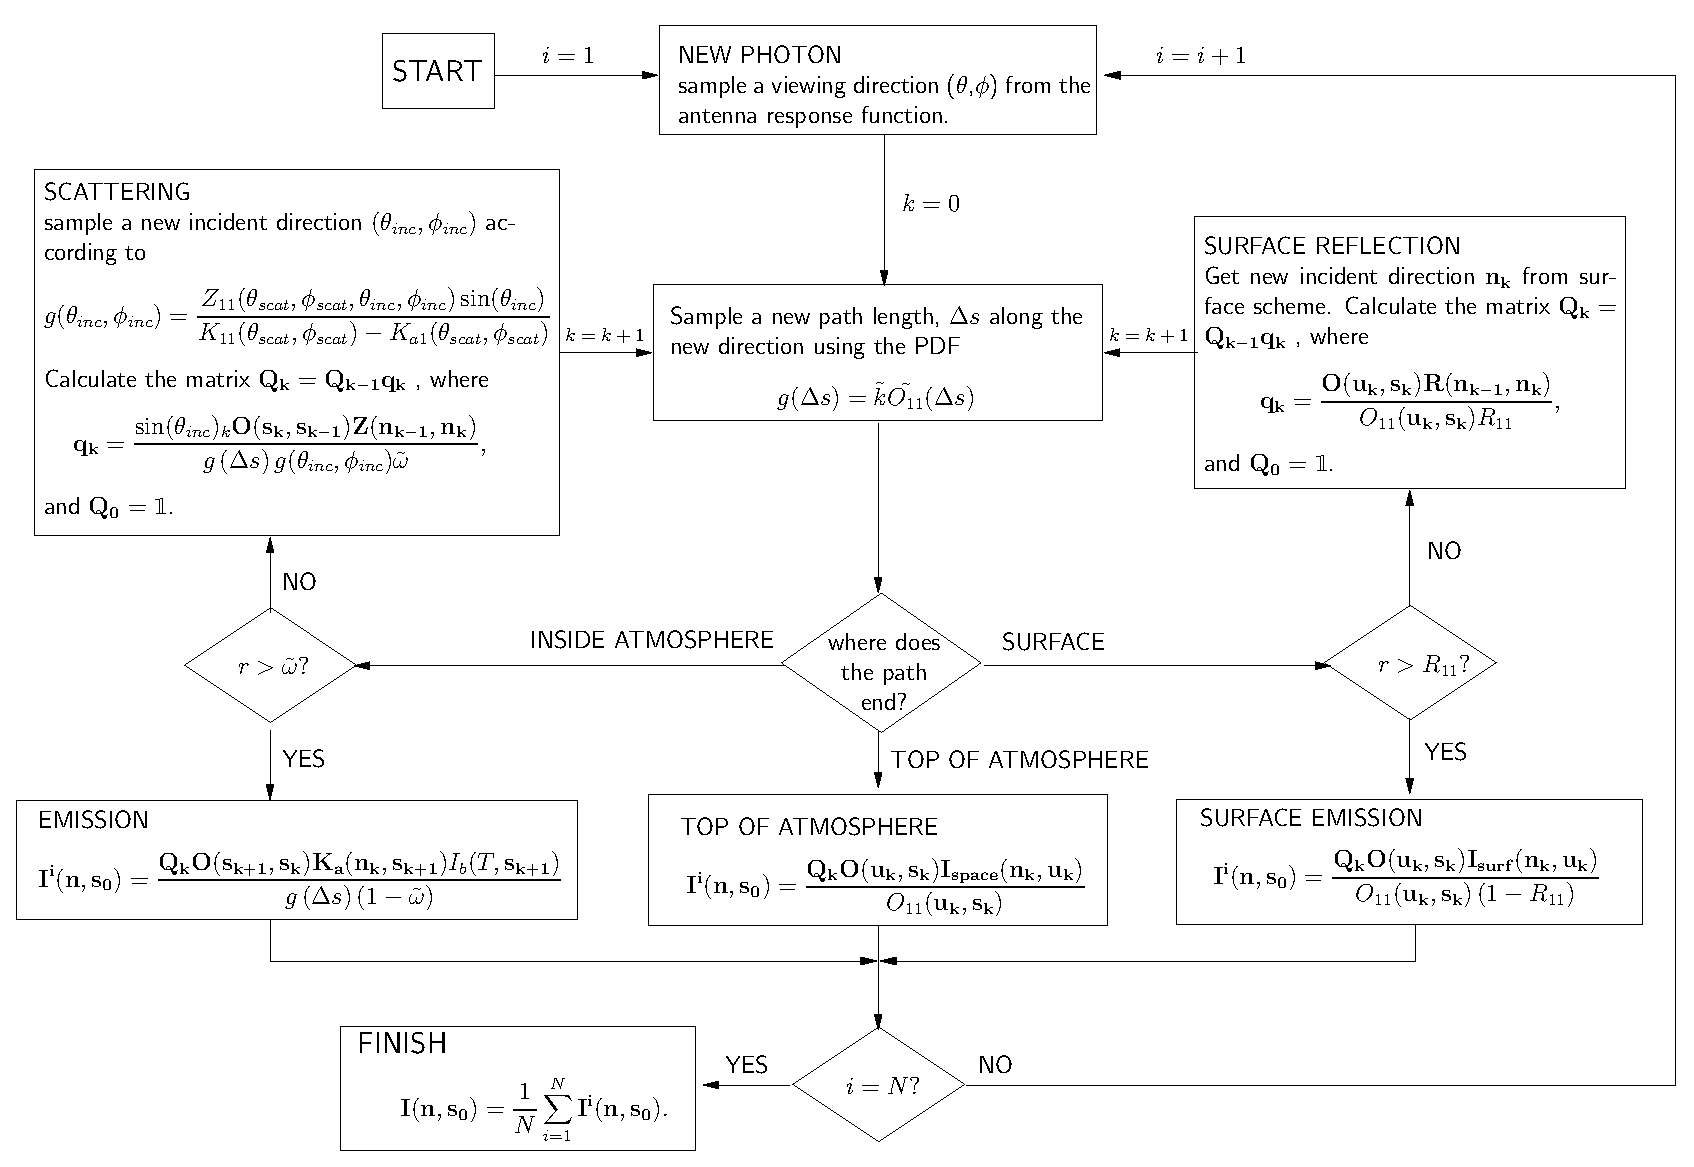
\includegraphics[width=\vsize,angle=90]{flowchart2}
\caption{Flowchart illustrating MCGeneral algorithm}
\end{center}
\zlabel{fig:montecarlo:flowchart}
\end{figure}

 
%%% Local Variables: 
%%% mode: latex 
%%% TeX-master: "uguide" 
%%% End:


%%
% To start the document, use
%  \chapter{...}
% For lover level, sections use
%  \section{...}
%  \subsection{...}
%
\chapter{Data reduction}
 \label{sec:red}


%
% Document history, format:
%  \starthistory
%    date1 & text .... \\
%    date2 & text .... \\
%    ....
%  \stophistory
%
\starthistory
  000321 & Created and written by Patrick Eriksson.\\
\stophistory


%
% Symbol table, format:
%  \startsymbols
%    ... & \verb|...| & text ... \\
%    ... & \verb|...| & text ... \\
%    ....
%  \stopsymbols
%
%
%\startsymbols
%  -- & -- & -- \\
% \label{symtable:red}     
%\stopsymbols



%
% Introduction
%
Many observation scenarios give rise to very large measurement
vectors, larger than can be handled practically during the inversions,
and some kind of reduction of the data size is needed. This data
reduction can be made part of the sensor transfer matrix. In fact, the
data reduction can be viewed upon as an imaginary second spectrometer.
The transfer matrix to use is then (Eq. \ref{eq:formalism:Hs})
\begin{eqnarray}
  \Hm = \Hd \Hs  \nonumber
\end{eqnarray}
where \Hd\ is the data reduction matrix and \Hs\ the sensor matrix.
{\it Data reduction can so far only be performed in Qpack.}


\section{Averaging of viewing angles}
 \label{sec:red:view}
 
 In some cases the spectra from different viewing angles are combined,
 either as a pure data reduction or internally in the spectrometer.
 The rows of \Hd\ for this case have the structure
 \begin{equation}
   \mat{h} = \big[ 0,\dots,0,\frac{1}{n_v},0,\dots,0,\frac{1}{n_v},0,\dots,0,\frac{1}{n_v},0,\dots,0\big]
 \end{equation}
 where $n_v$ is the number of viewing angles to combine.


\section{Data binning}
 \label{sec:red:binning}
 
 Data binning means that neighboring channels are combined by
 weighted averaging. If channels $i_1$ to $i_2$ of $\y'$ are combined to
 give element $j$ of $\y$, the binning can be expressed as
 \begin{equation}
   \y^j = \frac{1}{\sum_{i=i_1}^{i_2}{\Delta \f^i}} \sum_{i=i_1}^{i_2}{\Delta \f^i (\y')^i}
 \end{equation}
 Row $j$ of \Hd\ is accordingly
 \begin{equation}
   \mat{h}^i = \frac{\Delta \f^i}{\sum_{i=i_1}^{i_2}{\Delta \f^i}}, \qquad
    i_1\leq i \leq i_2
 \end{equation}
 Other values of $\mat{h}$ are zeros. The matrix \Hd\ is for data
 binning highly sparse.



\section{Reduction by eigenvectors}
 \label{sec:red:eig}
 
 A commonly used approach for reducing data sizes is to base the
 reduction of the eigenvectors of the covariance matrix expressing the
 variability of the measurements. These empirical eigenvectors
 fulfills the relationships
 \begin{equation}
   \mat{S}_\y = \mat{E}\Lambda\mat{E}^T
 \end{equation}
 where $\Lambda$ is a diagonal matrix holding the eigenvalues
 corresponding to the eigenvectors, the columns of $\mat{E}$. The
 eigenvectors form an orthogonal basis:
 \begin{equation}
   \Id = \mat{E}^T_j\mat{E}_j
 \end{equation}
 where $\mat{E}_j$ signifies the $j$ first columns of the matrix.

 The data reduction for this case is performed as
 \begin{equation}
   \y = \mat{E}^T_j \y'
 \end{equation}
 that is
 \begin{equation}
   \Hd = \mat{E}^T_j 
 \end{equation}
 By basing the data reduction on the covariance matrix eigenvectors,
 the reduction maintaining the maximum possible fraction of the
 variability of the spectra, for a given $j$, is achieved.

 Different versions of this scheme are described in \citet{eriksson:01c}. 
 The existing options in Qpack are described in the file \verb|README|.





%%% Local Variables: 
%%% mode: latex
%%% TeX-master: "uguide"
%%% End: 

%\graphicspath{{Figs/wfuns_atm/}}

%
% To start the document, use
%  \chapter{...}
% For lover level, sections use
%  \section{...}
%  \subsection{...}
%
\chapter{Atmospheric weighting functions}
 \label{sec:wfuns}


%
% Document history, format:
%  \starthistory
%    date1 & text .... \\
%    date2 & text .... \\
%    ....
%  \stophistory
%
\starthistory
  000310 & Started by Patrick Eriksson.\\
  000911 & First version finished by Patrick Eriksson.\\
\stophistory


%
% Symbol table, format:
%  \startsymbols
%    ... & \verb|...| & text ... \\
%    ... & \verb|...| & text ... \\
%    ....
%  \stopsymbols
%
%
%\startsymbols
%  -- & -- & -- \\
% \label{symtable:wfuns}     
%\stopsymbols



%
% Introduction
%
This section describes how the calculation of the atmospheric weighting
functions (WFs) matrices is performed in the forward model. For
several types of variables (such as species profiles and fit of
absorption continuum) WFs are obtained by semi-analytical expressions,
while for other quantities the WFs are obtained by straightforward
perturbation calculations.



\section{Calculation approaches}
 \label{sec:wfuns:approaches}

  \subsection{Pure numerical calculation} 
  The most straightforward method to determine WFs is by perturbing
  one parameter at a time. For example, the WF for the state variable
  $p$ can always be calculated as
  \begin{equation}
    \K_{\xt}^p = \frac{\fm(\xt+\Delta\xt^p\mat{e}^p,\bt)-\fm(\xt,\bt)}
                                     {\Delta\xt^p}
   \label{eq:wfuns:perturb}
  \end{equation}
  where $\K_{\xt}^p$ is column $p$ of \Kx, $(\xt,\bt)$ is the
  linearization state, $\mat{e}^p$ is a vector of zeros except for the
  component $p$ that is unity, and $\Delta\xt^p$ is a small disturbance
  (but sufficiently large to avoid numerical instabilities).
  
  However, it is normally not needed to make a recalculation using the
  total forward model as the variables are in general either part of the
  atmospheric or the sensor state, but not both. If $\xt^p$ is an atmospheric
  variable, the calculation can be performed as (Eq. \ref{eq:formalism:kx2})
  \begin{equation}
    \K_{\xt}^p = \Hm \bigg[
    \frac{\fm_r(\xt_r+\Delta\xt^p\mat{e}^p,\bt_r)-
           \fm_r(\xt_r,\bt_r)}  {\Delta\xt^p} \bigg]
   \label{eq:wfuns:Hpert}
  \end{equation}
  where $\xt_r$ is the atmospheric part of the state vector etc (see
  further Sec. \ref{sec:formalism}).
 

  \subsection{Analytical expressions} 
  \label{sec:wfuns:approaches:anal}
  For some atmospheric variables, such as species abundance, it is
  possible to derive a semi-analytical expression for the WFs. This is
  advantageous because it results in faster and more accurate
  calculations. By Equation \ref{eq:formalism:kx2},
  \begin{eqnarray*}
    \Kx = \Hm\frac{\partial\iv}{\partial \xt},
  \end{eqnarray*}
  it can be seen that the core problem of finding these analytical
  expressions is to determine $\partial\iv / \partial \xt$. 
  If $\xt^p$ influences only the conditions at one altitude, the
  problem can be simplified as \citep[][Eq. 43]{eriksson:00a}
  \begin{equation}
    \K_{\xt}^p = \Hm \frac{\partial\iv}{\partial \xt^p} = 
      \Hm \Bigg[ \frac{\partial\iv}{\partial \mat{S}^p}
                 \frac{\partial \mat{S}^p}{\partial \xt^p} +
                 \frac{\partial\iv}{\partial \mat{k}^p}
                 \frac{\partial \mat{k}^p}{\partial \xt^p} \Bigg]
   \label{eq:wfuns:taylor}
  \end{equation}
  where $\mat{S}^p$ and $\mat{k}^p$ are the source function and the
  absorption at the (vertical) altitude $p$, respectively.
  
  It is very important to note that the analytical expressions are
  derived with the assumption that $\xt^p$ influences only the local
  conditions. For species it is further assumed that the absorption
  can be expressed as (see Section \ref{sec:wfuns:species} for
  definitions and details)
  \begin{equation}
   \mat{k}^p = \mat{\bar{k}}^p_s \xt^p + \sum_{i\ne s} \mat{k}^p_i
  \end{equation}
  These assumption should be of general validity
  for species above the tropopause. Two examples on when the
  analytical expressions will be approximative are
  \begin{itemize}
  \item The variable of interest can change the line-of-sight (by the
    refractive index). This is an example of a non-local effect. This
    is always valid for temperature.
  \item The amount of different species must be considered when
    calculating the pressure broadening, and not only the total
    absorption.
  \end{itemize}
  If the analytical expressions can be used for such cases must be
  tested numerically. When it is found that the analytical approach
  cannot be used, the WFs must be calculated by perturbations to
  include the neglected effects (such a function for species is not
  yet implemented in ARTS). An important example when these questions
  must be considered is limb sounding of water vapor in the
  troposphere where both points above are true. The abundance of water
  in the troposphere is sufficient high to have a significant
  influence on both the refractive index and the pressure broadening.
  These questions are discussed somewhat further in \citet{eriksson:01d}.

  The absorption and source function in Equation \ref{eq:wfuns:taylor}
  are defined in vertical coordinates (as we retrieve atmospheric
  variables as functions of altitude). For different reasons it is
  more practical to work with these quantities defined along the LOS.
  For example, the source function and transmission along the LOS are
  already determined when calculating the spectra. To solve this
  problem, Equation \ref{eq:wfuns:taylor} is expanded one step further
  \begin{equation}
    \K_{\xt}^p = \Hm \Bigg[ \frac{\partial\iv}{\partial \sigma}
                 \frac{\partial \sigma}{\partial \mat{S}^p} 
                 \frac{\partial \mat{S}^p}{\partial \xt^p} +
                 \frac{\partial\iv}{\partial \kappa}
                 \frac{\partial \kappa}{\partial \mat{k}^p}
                 \frac{\partial \mat{k}^p}{\partial \xt^p} \Bigg]
   \label{eq:wfuns:taylor2}
  \end{equation}
  where $\sigma$ and $\kappa$ are the source function and the absorption 
  along the LOS, respectively.
  
  The term $\partial\iv / \partial \sigma$ is here denoted as source
  line of sight weighting functions (source LOS WFs) and is discussed
  in Section \ref{sec:wfuns:sourceloswfs}. The term $\partial\iv/
  \partial \kappa$ is denoted as absorption LOS WFs and is discussed
  in Sections \ref{sec:wfuns:absloswfs} and
  \ref{sec:wfuns:absloswfs2}. These terms are treated separately as
  they are common for all variables influencing the source function or
  the absorption.

  The term $\partial \mat{S}^p/\partial \xt^p$ can often be neglected.
  When scattering is neglected and local thermodynamic equilibrium is
  assumed, the only variable of interest affecting the source function
  is the temperature.  See further Section \ref{sec:wfuns:temp}. For
  other variables, such as species abundance, $\partial
  \mat{S}^p/\partial \xt^p=0$.
  
  It was decided to allow that the retrieval grids differ between
  species, temperature etc. This results in that the terms $\partial
  \sigma/ \partial \mat{S}^p$ and $\partial \kappa/ \partial
  \mat{k}^p$ are not constant, they change according to the selected
  retrieval grid. Accordingly, it is not suitable to include these terms
  in the corresponding LOS WFs, they must be treated separately.
  
  

\section{Absorption LOS WFs with emission}
 \label{sec:wfuns:absloswfs}

 The absorption line of sight weighting functions are defined as
 \begin{equation}
   \K_{\kappa}^q =  \frac{\partial\iv}{\partial \kappa^q}
  \label{eq:wfuns:loswfs}
 \end{equation}
 These weighting functions express how the intensity is
 affected by changes of the absorption at the points of the line of
 sight. Note that $\kappa$ is the total absorption, not the
 absorption of a single species. 
 
 For simplicity, the absorption LOS WFs are below derived without
 using vector notation. The notation used here is identical to the one
 used in Section \ref{sec:rte}. The calculation approach used for the
 LOS WFs is ``inspired'' by the corresponding work in
 \citet{master00}.


 \subsection{Single pass}
 \label{sec:wfuns:single}
 
 This section derives the absorption LOS WFs for cases when each
 individual part of the atmosphere is passed only once, as for upward
 looking measurements, or when each point in the atmosphere is treated
 separately (2D simulations). With other words, the conditions are not
 assumed to be symmetrical around some point. Accordingly, 1D limb
 sounding and 1D downward observations are not treated here, and are
 instead discussed in Section \ref{sec:wfuns:limb} and
 \ref{sec:wfuns:down}, respectively.

 \begin{figure}[t]
  \begin{center}
   \includegraphics*[width=0.95\hsize]{wf1}
   \caption{The terms used for the derivation of line of sight weighting
            functions when the individual atmospheric parts are passed a
            single time. The variables are defined in Figure 
            \ref{fig:rte:los}.}
   \label{fig:wfuns:single}  
  \end{center}
 \end{figure}

 By rewriting Equation \ref{eq:rte:rteprod}, the monochromatic pencil beam
 intensity can be expressed in the following ways (see Fig. 
 \ref{fig:wfuns:single})\footnote{The indexing used here is 1-based 
  (starts at 1), while inside ARTS 0-based indexing is used.}
 \begin{eqnarray}
   I &=& I_2\zeta_1+\psi_1(1-\zeta_1) \quad (q=1) 
     \nonumber \\
   I &=&\Big[I_{q+1}\zeta_q\zeta_{q-1}+\psi_q(1-\zeta_q)\zeta_{q-1} +
            \psi_{q-1}(1-\zeta_{q-1}) \Big] \Theta^{q-1}_1, \quad 1<q<n 
    \label{eq:wfuns:mpbi} \\
   I &=& \Big[I_n\zeta_{n-1}+\psi_{n-1}(1-\zeta_{n-1})\Big]\Theta^{n-1}_{1}
     \quad (q=n)
     \nonumber
 \end{eqnarray}
 where it assumed that the LOS has $n$ points, index 1 is the point
 closest to the sensor,
 \begin{equation}
   I_q = I_n \Theta^{n}_{q} + \sum_{i=q}^{n-1}\psi_i(1-\zeta_i) 
             \Theta_{q}^{i}, \quad 1 \leq q < n
  \label{eq:wfuns:iq}
 \end{equation}
 is the intensity reaching point $q$ along the LOS, $I_n$ is the radiation at
 point n (the radiation entering the atmosphere), and
 \begin{equation}
   \Theta_q^p = \prod_{i=q}^{p-1}\zeta_i\quad \mathrm{for} \quad p>q, 
     \quad \mathrm{and} \quad \Theta_p^p = 1
  \label{eq:wfuns:Theta}
 \end{equation}
 the transmission from point $q$ and $p$. It should be noted that
 $I_q$ and $\Theta_q^p$ not are calculated as indicated by the
 equations above. These quantities are instead updated when going from
 one step of the LOS to the next, as described below. It should also be
 noted that ground reflections are here neglected and are discussed 
 separately below.

 The transmissions $\zeta_{q-1}$ and $\zeta_q$ are separated in Equation
 \ref{eq:wfuns:mpbi} as they are the only terms including the absorption
 at point $q$. For example
 \begin{equation}
   \zeta_{q-1} = e^{-\Delta l(\kappa_{q-1}+\kappa_q)/2}
 \end{equation}
 and we have that
 \begin{equation}
   \frac{\partial \zeta_q}{\partial \kappa_q} = -\frac{\Delta l}{2}\zeta_q
  \label{eq:wfuns:dzeta1}
 \end{equation}
 \begin{equation}
   \frac{\partial\zeta_{q-1}}{\partial \kappa_q}=-\frac{\Delta l}{2}\zeta_{q-1}
 \end{equation}
 \begin{equation}
   \frac{\partial \zeta_{q-1}\zeta_q}{\partial \kappa_q} = 
          -\Delta l \zeta_{q-1}\zeta_q
  \label{eq:wfuns:dzeta2}
 \end{equation}
 The derivate of transmission values beside $\zeta_q$ and
 $\zeta_{q-1}$ with respect to $\kappa_q$ is zero.

 The LOS WFs are now easily determined, using the case $1<q<n$ as example
 \begin{equation}
   \K_{\kappa}^q = -\frac{\Delta l}{2} \Big[ 2I_{q+1}\zeta_q\zeta_{q-1}+
     \psi_q(1-2\zeta_q)\zeta_{q-1} - \psi_{q-1}\zeta_{q-1} \Big] 
     \Theta^{q-1}_1, \, 1<q<n
 \end{equation}
 which can be rewritten as
 \begin{eqnarray}
   \K_{\kappa}^1 &=& -\frac{\Delta l}{2} \big[ I_2-\psi_1 \big] \Theta^2_1 \nonumber \\
   \K_{\kappa}^q &=& -\frac{\Delta l}{2} \big[ 2(I_{q+1}-\psi_q)\zeta_q+
           \psi_q-\psi_{q-1} \big] \Theta^q_1, \quad 1<q<n 
  \label{eq:wfuns:loswfsxx} \\
   \K_{\kappa}^n &=& -\frac{\Delta l}{2} \big[ I_n-\psi_{n-1} \big] \Theta^n_1 \nonumber
 \end{eqnarray}
 Note that one $\zeta_q$ is incorporated in $\Theta^q_q$, and that 
 $\Theta^2_1=\zeta_1$.
 
 These equations are used for the practical calculations, but it could
 be of interest to note that Equation \ref{eq:wfuns:loswfsxx} can be
 written
 \begin{equation}
   \K_{\kappa}^q = -\frac{\Delta l}{2} \big[ (I_{q+1}-\psi_q)\zeta_q+
           I_q-\psi_{q-1} \big] \Theta^q_1, \quad 1<q<n ,
 \end{equation}
 showing that the expressions for $q=1$ and $q=n$ are special cases of
 the general expression where the terms connected to $q-1$ and $q$,
 are neglected, respectively.
 
 The iteration starts here at the end closest to the
 sensor, that is, at index 1 (reversed order to the RTE part).  The
 iteration is started by setting $I_1$ to the already calculated
 spectrum and $\Theta^1_1$ to 1.  These two variables are updated as
 \begin{eqnarray}
   I_{q+1} = \frac{I_q - \psi_q(1-\zeta_q)}{\zeta_q} 
 \end{eqnarray}
 \begin{eqnarray}
   \Theta_1^{q+1} =  \Theta_1^q \zeta_q
 \end{eqnarray}
 For 2D calculations possible ground reflections inside the LOS must
 be handled. The ground cannot be found at any of the end points of
 the LOS, and the correspondence to Equation \ref{eq:wfuns:mpbi} for a
 ground point is (c.f. Equations \ref{eq:rte:ground} and
 \ref{eq:rte:tground})
 \begin{eqnarray}
   I &=&\Big[I_{q+1}\zeta_q(1-e)\zeta_{q-1}+\psi_q(1-\zeta_q)(1-e)\zeta_{q-1}
          +eB\zeta_{q-1}+ \nonumber \\
     & & + \psi_{q-1}(1-\zeta_{q-1}) \Big] \Theta^{q-1}_1, \quad 1<q<n 
    \label{eq:wfuns:mpbi_ground}
 \end{eqnarray}
 and the corresponding absorption LOS WF for this point is (cf. Eq.
 \ref{eq:wfuns:loswfsxx})
 \begin{eqnarray}
   \K_{\kappa}^q &=& -\frac{\Delta l}{2} \big[ 2(I_{q+1}-\psi_q)\zeta_q(1-e)+
           \psi_q(1-e)+eB-\psi_{q-1} \big] \Theta^q_1 
 \end{eqnarray}
 The intensity and the transmission are here updated as
 \begin{eqnarray}
   I_{q+1} &=& \frac{I_q-\psi_q(1-\zeta_q)(1-e)-eB}{\zeta_q(1-e)}  \nonumber \\
   \Theta_1^{q+1} &=& \Theta_1^{q}\zeta_q(1-e) \nonumber
 \end{eqnarray}
 It is noteworthy that the effect of a ground intersection is included
 in $I_1$ when the iteration starts.  


 
 \subsection{1D limb sounding}
 \label{sec:wfuns:limb}
    
 For limb sounding and when the atmosphere is assumed to be consist of
 homogenous layers (horizontally stratified), there is a perfect
 symmetry around the tangent point. This covers also the case with a
 ground reflection. For these cases the distance from the sensor is
 neglected, the important factor is the vertical altitude.  All
 altitudes above the tangent point are passed twice (Fig.
 \ref{fig:wfuns:limb}) and both crossings of an atmospheric layer are
 treated to be identical for the retrievals, and this fact must also
 be reflected by the WFs.

 Using a nomenclature similar to the one used for Equation
 \ref{eq:wfuns:mpbi}, the intensity of a limb sounding
 observations can be expressed as (Fig. \ref{fig:wfuns:limb})
 \begin{eqnarray}
   I & = & \Big(I_2 \Big( \zeta_1\Theta^1_1 \Big)^2 + \psi_1(1-\zeta_1)
            \Big( \Theta^1_1 \Big)^2 \zeta_1+
            I_1^1\zeta_1+\psi_1(1-\zeta_1) \Big)\Theta^n_{2} \quad (q=1) 
        \nonumber \\
   I & = & \Big[\Big(I_{q+1}\zeta_q\zeta_{q-1} +\psi_q(1-\zeta_q)\zeta_{q-1} + 
           \psi_{q-1}(1-\zeta_{q-1})\Big)\Big(\Theta^{q-1}_{1}\Big)^2
           \zeta_{q-1}\zeta_q + \nonumber \\
      & & + I_{q-1}^{q-1}\zeta_{q-1}\zeta_q + \psi_{q-1}(1-\zeta_{q-1})
           \zeta_q + \psi_q(1-\zeta_q) \Big] \Theta^n_{q+1}, \, 1<q<n
  \label{eq:wfuns:limb1}  \\
   I & = & \Big(I_n\zeta_{n-1}+\psi_{n-1}(1-\zeta_{n-1})\Big)\Big
           (\Theta^{n-1}_{1}\Big)^2\zeta_{n-1} + I_{n-1}^{n-1}\zeta_{n-1} +
             \nonumber \\
      & &  +   \psi_{n-1}(1-\zeta_{n-1}) \quad (q=n) \nonumber
 \end{eqnarray}
 where the expression for $q=1$ is commented below, index 1 of the LOS
 is the tangent (or the ground) point, index $n$ corresponds to the
 highest altitude,
 \begin{equation}
   I_q = I_n \Theta^{n}_{q} + \sum_{i=q}^{n-1}\psi_i(1-\zeta_i) 
             \Theta_{q}^{i-1}
  \label{eq:wfuns:iqq}
 \end{equation}
 is the intensity reaching point $q$ from the part of the
 atmosphere furthest away from the sensor, $I_n$ the intensity at point $n$,
 \begin{equation}
   I_q^q = \Big[ \sum_{i=1}^{q-1}(\psi_i(1-\zeta_i)\Theta_{1}^{i-1}\Big]
             \Theta_{1}^{q} + \sum_{i=1}^{q-1}\psi_i(1-\zeta_i)
            \Theta_{i+1}^{q}, \qquad q>1
 \end{equation}
 is the intensity generated along the LOS (towards the sensor) between
 the two crossing with altitude $q$, $I_1^1=0$, $\Theta$ is defined by
 Equation \ref{eq:wfuns:Theta}. The equations defining $I_q$, $I_q^q$
 and $\Theta$ neglect ground reflections, but could easily be extended
 to cover also such cases. However, $I_1^1$ and $\Theta_1^1$ are
 included for $q=1$ to make Equation \ref{eq:wfuns:limb1} valid for
 cases with ground reflections. The treatment of ground reflections
 are discussed separately last in the section.

 \begin{figure}[tb]
  \begin{center}
   \includegraphics*[width=0.95\hsize]{wf2}
   \caption{The terms used for the derivation of line of sight weighting
            functions for 1D limb sounding.}
   \label{fig:wfuns:limb}  
  \end{center}
 \end{figure}
 
 If the different combinations of $\zeta_{q-1}$ and $\zeta_q$ are 
 grouped, for example, Equation \ref{eq:wfuns:limb1} becomes
 \begin{eqnarray}
   I & = & \Big[\Big((I_{q+1}-\psi_q)\zeta_{q-1}^2\zeta_q^2+(\psi_q-\psi_{q-1})
            \zeta_{q-1}^2\zeta_q + \psi_{q-1}\zeta_{q-1}\zeta_q
            \Big)\Big(\Theta^{q-1}_{1}\Big)^2 + \nonumber \\
    &  &     + (I_{q-1}^{q-1}-\psi_{q-1})\zeta_{q-1}\zeta_q + 
            (\psi_{q-1}-\psi_q)\zeta_q + \psi_q \Big] \Theta^n_{q+1} 
 \end{eqnarray}
 This equation has some higher products between
 $\zeta_{q-1}$ and $\zeta_q$ than Equation \ref{eq:wfuns:mpbi}, and
 the derivatives, with respect to $\kappa_q$, of these product are
 \begin{equation}
   \frac{\partial \zeta_{q-1}^2\zeta_q}{\partial \kappa_q} = 
         -\frac{3\Delta l}{2} \zeta_{q-1}^2\zeta_q
  \label{eq:wfuns:dzeta3}
 \end{equation}
 \begin{equation}
   \frac{\partial \zeta_{q-1}^2\zeta_q^2}{\partial \kappa_q} = 
          -2\Delta l \zeta_{q-1}^2\zeta_q^2
  \label{eq:wfuns:dzeta4}
 \end{equation}
 Using Equations \ref{eq:wfuns:dzeta1}, \ref{eq:wfuns:dzeta2},
 \ref{eq:wfuns:dzeta3} and \ref{eq:wfuns:dzeta4}, the LOS WFs for 1D
 limb sounding can be determined to be
 \begin{eqnarray}
   \K_{\kappa}^1& = & -\frac{\Delta l}{2}\Big[ \Big( 2I_2\zeta_1+\psi_1(1-
       2\zeta_1)\Big) \Big(\Theta^1_1\Big)^2 +I_1^1-\psi_1 \Big]\Theta^n_1
          \nonumber \\
   \K_{\kappa}^q& = & -\frac{\Delta l}{2}\Big[\Big(4(I_{q+1}-\psi_q)
           \zeta_{q-1}\zeta_q+
            3(\psi_q-\psi_{q-1})\zeta_{q-1} + 2 \psi_{q-1}
            \Big) \Big(\Theta^{q-1}_{1}\Big)^2\zeta_{q-1}  \nonumber \\
       &  & + 2(I_{q-1}^{q-1}-\psi_{q-1})\zeta_{q-1} + 
            \psi_{q-1}-\psi_q \Big] \Theta^n_{q}, \quad 1<q<n
  \label{eq:wfuns:loswfs2} \\
   \K_{\kappa}^n& = & -\frac{\Delta l}{2}\Big[\Big( 2I_n\zeta_{n-1}+
         \psi_{n-1}(1-2\zeta_{n-1}) \Big)\Big(\Theta^{n-1}_{1}\Big)^2\zeta_{n-1}+ 
             \nonumber \\   
       & &  + I_{n-1}^{n-1}-\psi_{n-1}\Big] \zeta_{n-1} \nonumber
 \end{eqnarray}
 The function calculating these LOS WFs takes the total spectrum as
 input (that is, $I_n^n$) and it is then most suitable to iterate
 downwards, starting with point $n$. For each iteration, the
 quantities are updated as
 \begin{eqnarray}
   I_q = I_{q+1}\zeta_q + \psi_q(1-\zeta_q) \nonumber
 \end{eqnarray}
 \begin{eqnarray}
   \Theta_{1}^{q-1} =  \frac{\Theta_{1}^{q}}{\zeta_{q-1}} \nonumber
 \end{eqnarray}
 \begin{eqnarray}
   I_{q-1}^{q-1} = \frac{I_q - \psi_{q-1}(1-\zeta_{q-1})
       (1+\big(\Theta^{q-1}_{1}\big)^2\zeta_{q-1})}{\zeta_{q-1}} \nonumber
 \end{eqnarray}
 The iteration is started by setting $I_n$ to cosmic
 background radiation, or correspondingly, and setting
 $\Theta^n_1$ to the square root of the total transmission. As
 mentioned above, $I_n^n$ is an input to the function.
 
 No special attention needs to be given here to possible ground
 reflections.  This as the effects of a ground reflection are already
 included in $I_n^n$ and $\Theta^n_1$ when starting the iteration. The
 procedure of setting $\Theta^n_1$ to the square root of the total
 transmission maintains the symmetry and makes it possible to treat
 the ground as an imaginary altitude ``below'' point 1. If there is a
 ground reflection, $\Theta^1_1$ and $I_1^1$ equal $\sqrt{1-e}$ and
 $eB$, respectively, at the end of the iteration.


 

 \subsection{1D downward looking observations}
  \label{sec:wfuns:down}
  Downward observation from an aircraft or a balloon can mainly be
  treated as a combination of limb sounding and upward looking
  observations.  The altitudes below the platform altitude are covered
  by the limb sounding expressions with a suitable choice of $I_q$ for
  the highest point. The altitudes above the platform altitude are
  treated by the upward looking equations, but also considering the
  transmission through the lower altitudes. 
  
  If $q$ is the index for platform altitude, the intensity can be
  expressed as
  \begin{eqnarray}
   I &=& \Big(I_{q+1}\zeta_q\zeta_{q-1} +\psi_q(1-\zeta_q)\zeta_{q-1} + 
           \psi_{q-1}(1-\zeta_{q-1})\Big)\Big(\Theta^{q-1}_{1}\Big)^2
           \zeta_{q-1} + \nonumber \\
      & & + I_{q-1}^{q-1}\zeta_{q-1} + \psi_{q-1}(1-\zeta_{q-1})
    \label{eq:wfuns:idown}
  \end{eqnarray}
  and the corresponding WF is
  \begin{eqnarray}
   \K_{\kappa}^q& = & -\frac{\Delta l}{2}\Big[\Big(3(I_{q+1}-\psi_q)
           \zeta_{q-1}\zeta_q+ 2(\psi_q-\psi_{q-1})\zeta_{q-1} + \psi_{q-1} \Big)
           \Big(\Theta^{q-1}_{1}\Big)^2 + \nonumber \\
      & &  + I_{q-1}^{q-1}-\psi_{q-1}\Big]\zeta_{q-1}
  \end{eqnarray}



\section{Absorption LOS WFs for optical thicknesses}
 \label{sec:wfuns:absloswfs2}

 This section treats the absorption LOS WFs for cases when emission
 can neglected. For such pure absorption calculations the output
 of ARTS is optical thicknesses (instead of e.g. transmissions) and
 for these conditions the absorption LOS WFs get very simple.

 \subsection{Single pass}
 The optical thickness $(\tau)$ is for single pass cases (cf. Eq. 
 \ref{eq:rte:tau})
 \begin{equation}
   \tau = \Delta l \left( \frac{\kappa_1+\kappa_2}{2} +
                          \frac{\kappa_2+\kappa_3}{2} + \dots +
                          \frac{\kappa_{n-2}+\kappa_{n-1}}{2} +
                          \frac{\kappa_{n-1}+\kappa_n}{2} \right)
 \end{equation}
 and we have that
 \begin{eqnarray}
   \K_{\kappa}^1& = & \Delta l / 2 \nonumber \\
   \K_{\kappa}^q& = & \Delta l, \quad 1<q<n  \\
   \K_{\kappa}^n& = & \Delta l / 2 \nonumber
 \end{eqnarray}


 \subsection{1D limb sounding}
 For limb sounding each altitude is passed twice and the total optical 
 thickness is double the optical thickness from the tangent point to the
 atmospheric limit. This fact results in that the absorption LOS WFs
 for 1D limb sounding are just the single pass ones multiplicated by two:
 \begin{eqnarray}
   \K_{\kappa}^1& = & \Delta l  \nonumber \\
   \K_{\kappa}^q& = & 2 \Delta l, \quad 1<q<n  \\
   \K_{\kappa}^n& = & \Delta l  \nonumber
 \end{eqnarray}
 

 \subsection{1D downward looking observations}
 If $q$ is the point where the sensor is placed, the optical thickness
 is
 \begin{equation}
   \tau = \Delta l \left( \frac{\kappa_q+\kappa_{q-1}}{2} + \dots+
                          \frac{\kappa_2+\kappa_1}{2} + \dots +
                          \frac{\kappa_{q-1}+\kappa_q}{2} +
                          \frac{\kappa_q+\kappa_{q+1}}{2} \dots \right)
 \end{equation}
 and the absorption LOS WF for this altitude is accordingly
 \begin{equation}
   \K_{\kappa}^q =  \frac{3}{2} \Delta l
 \end{equation}





\section{Source line of sight weighting functions}
 \label{sec:wfuns:sourceloswfs}

 The source line of sight weighting functions are defined as
 \begin{equation}
   \K_{\sigma}^q =  \frac{\partial\iv}{\partial \sigma^q}
  \label{eq:wfuns:sloswfs}
 \end{equation}
 These weighting functions express how the intensity is affected by
 changes of the source function at the points of the line of sight.
 The source and absorption LOS WFs are tightly related and this
 section follows closely Section \ref{sec:wfuns:absloswfs}.


 \subsection{Single pass}
  \label{sec:wfuns:single2}
  As, for example,
  \begin{equation}
    \psi_{q} = \frac{\sigma_q+\sigma_{q+1}}{2}
  \end{equation}
  the derivate of the mean source function values with respect to 
  $\sigma_q$ is
  \begin{equation}
    \frac{\partial \psi_{q-1}}{\partial \sigma_q} = 
    \frac{\partial \psi_q}{\partial \sigma_q} = \frac{1}{2}
   \label{eq:wfuns:dpsi}
  \end{equation}
  This derivate for other $\psi$ terms is zero.
 
  Using \ref{eq:wfuns:mpbi}, the source LOS WFs for upward looking
  observations can be determined to be
  \begin{eqnarray}
    \K_{\sigma}^q &=& \frac{1-\zeta_1}{2}, \quad q=1 
     \nonumber \\
    \K_{\sigma}^q &=& \frac{1-\zeta_{q-1}\zeta_q}{2} 
                                            \Theta^{q-1}_1, \quad 1<q<n \\
    \K_{\sigma}^q &=& \frac{1-\zeta_{n-1}}{2}\Theta^{n-1}_{1}, \quad q=n
     \nonumber
  \end{eqnarray}
  For ground points in 2D calculations, the WFs are (cf. Eq. 
  \ref{eq:wfuns:mpbi_ground})
  \begin{equation}
    \K_{\sigma}^q = \frac{(1-\zeta_q)(1-e)\zeta_{q-1}+1-\zeta_{q-1}}{2} 
                                            \Theta^{q-1}_1, \quad 1<q<n \\
  \end{equation}
  The practical calculations, such as the updating of $\Theta$, follow the
  absorption LOS WFs (Sec. \ref{sec:wfuns:single}).


 \subsection{1D limb sounding}
  \label{sec:wfuns:limb2}
  The 1D limb sounding source LOS WFs are (derived using Eq.
  \ref{eq:wfuns:limb1})
  \begin{eqnarray}
    \K_{\sigma}^q & = & \frac{1}{2} \Big(1-\zeta_1\Big) \Big(1+
        \Big( \Theta^1_1 \Big)^2\zeta_1 \Big) \Theta^n_2, 
                                                    \quad q=1  \nonumber \\
    \K_{\sigma}^q & = & \frac{1}{2} \Big[ (1-\zeta_{q-1}\zeta_q)
           \Big(\Theta^{q-1}_{1}\Big)^2\zeta_{q-1}\zeta_q + 
           (1-\zeta_{q-1})\zeta_q + \nonumber \\
      & & + 1-\zeta_q \Big] \Theta^n_{q+1}, \quad 1<q<n \\
    \K_{\sigma}^q & = & \frac{1}{2} \Big( (1-\zeta_{n-1}) \Big(
           \Theta^{n-1}_{1}\Big)^2\zeta_{n-1} + 1-\zeta_{n-1} \Big), \quad q=n \nonumber
  \end{eqnarray}
  The practical calculations follow the absorption LOS WFs (Sec.
  \ref{sec:wfuns:limb}).


 \subsection{1D downward looking observations}
  \label{sec:wfuns:down2}
  The source LOS WFs for downward looking observations are determined
  by the upward and the limb sounding expressions in the same manner
  as for the absorption LOS WFs (Sec. \ref{sec:wfuns:down}).

  The LOS WF for the index corresponding to the platform altitude is
  (cf. Eq. \ref{eq:wfuns:idown})
  observations can be determined to be
  \begin{equation}
   \K_{\sigma}^q = \frac{1}{2}\Big[ (1-\zeta_{q-1}\zeta_q) 
           \Big(\Theta^{q-1}_{1}\Big)^2
           \zeta_{q-1} + 1-\zeta_{q-1} \Big]\
  \end{equation}



\section{Transformation from vertical altitudes to distances along LOS}
 \label{sec:wfuns:bases}
 
 \subsection{Basis functions} 
 The source function and the absorption, both
 as a function of vertical altitude $(\mat{k})$ and along the LOS
 $(\kappa)$, are assumed to vary linear between the points of the grid
 of concern. The functions to express the quantities between grid
 points are denoted as basis functions. For piecewise linear functions,
 the basis functions decline, from the point of interest, linearly
 down to zero at neighboring points. Such functions are here denoted
 as tenth functions (Fig. \ref{fig:wfuns:zbasis}).
 
 
 \subsection{Transformation from $z$ to $l$} 
 The forward model uses
 internally a grid along the line of sight (Sec. \ref{sec:los}), while
 the atmospheric WF matrices are calculated for some user specified
 vertical grid, and a transformation between these two grids must be
 performed. This transformation is achieved by the terms,
 $\partial\kappa/ \partial \mat{k}^p$ and $\partial \sigma / \partial
 S^\mat{p}$. As the source function and the absorption are assumed to
 have the same functional behaviour (piecewise linear), these two
 terms are identical if the retrieval grid is the same for both quantities:
 \begin{equation}
   \frac{\partial \kappa}{\partial \mat{k}^p} =
   \frac{\partial \sigma}{\partial S^\mat{p}}
  \label{eq:wfuns:sandk}
 \end{equation}
 \begin{figure}[t]
  \begin{center}
   \includegraphics*[width=0.7\hsize]{fig_absbasis_z}
   \caption{Examples on basis functions for a vertical grid with a 1 km
            spacing: \lsolid~30~km, \ldashed~31~km and \ldashdot~32~km.}
   \label{fig:wfuns:zbasis}  
  \end{center}
 \end{figure}
 \begin{figure}[t]
  \begin{center}
   \includegraphics*[width=0.7\hsize]{fig_absbasis_l}
   \caption{The basis functions of Figure \ref{fig:wfuns:zbasis} shown
            as a function of the distance from the tangent point, where
            $z_{tan}=30$ km.}
   \label{fig:wfuns:lbasis}  
  \end{center}
 \end{figure}
 For example, the term $\partial\kappa/ \partial \mat{k}^p$ gives the
 relationship between the absorption along the LOS and a change of the
 absorption at one altitude.  Figure \ref{fig:wfuns:lbasis}
 exemplifies $\partial\kappa/ \partial \mat{k}^p$ for three altitudes.
 Ideally, the following relationship should be fulfilled for all $z$
 \begin{equation}
   \sum_i\mat{k}^i\phi^i_\mat{k}(z(l)) = \sum_j \kappa^j\phi^j_{\kappa}(l)
  \label{eq:wfuns:bases}
 \end{equation}
 where $\phi_\mat{k}$ and $\phi_{\kappa}$ are the basis functions for
 $\mat{k}$ and $\kappa$, respectively. However, as can be seen in
 Figure \ref{fig:wfuns:lbasis}, $\phi^i_\mat{k}$ expressed along the
 LOS is not a piecewise linear function and cannot be fitted perfectly
 by the basis $\phi_{\kappa}$. Hence, some approximation is needed,
 and the most natural choice for this approximation is to fulfill
 Equation \ref{eq:wfuns:bases} only for the grid points along the LOS:
 \begin{equation}
   \kappa^q = \sum_i\mat{k}^i\phi^i_\mat{k}(z(\mat{l}^q))
 \end{equation}
 where $\mat{l}^q$ is the distance along the LOS for the corresponding to
 $\kappa^q$. Note that at $\mat{l}^q$ all $\phi_{\kappa}^j$ are zero except
 for $\phi_{\kappa}^q$, that is unity.

 We have now that
 \begin{equation}
   \frac{\partial \kappa^q}{\partial \mat{k}^p} = \phi^p_\mat{k}(z(\mat{l}^q))
  \label{eq:wfuns:kappak}
 \end{equation}
 Hence, term $\partial\kappa/ \partial \mat{k}^p$ is determined by the
 values of $\phi^p_\mat{k}$ at the altitudes corresponding to the grid
 points of the LOS.
 
 Assuming that the LOS altitude $q$, $z_{\kappa^q}$, is found between
 retrieval points $p-1$ and $p$, at the altitudes $z_{\mat{k}^{p-1}}$ and 
 $z_{\mat{k}^p}$, respectively, we have that
 \begin{equation}
   \frac{\partial \kappa^q}{\partial \mat{k}^p} =
   \frac{z_{\kappa^q}-z_{\mat{k}^{p-1}}}{z_{\mat{k}^{p}}-z_{\mat{k}^{p-1}}}
  \label{eq:wfuns:zz}
 \end{equation}
 If $z_{\kappa^q}$ is further away from $z_{\mat{k}^p}$ than the neighboring
 retrieval points, the derivative is zero. The derivative is also treated to 
 be zero if $z_{\kappa^q}$ is outside the retrieval grid (that is, below
 or above all retrieval altitudes).

 The basis functions for $\mat{k}$ change if the retrieval grid is
 changed, and as the retrieval grid is individual for the species, 
 temperature etc., the term $\partial\kappa/ \partial \mat{k}^p$ 
 must be determined for each calculation of a WF matrix.


\section{Species WFs}
 \label{sec:wfuns:species}
 
 As it is assumed here that the species have no influence on
 the source function, species WFs are calculated as (cf. Eq.
 \ref{eq:wfuns:taylor2})
 \begin{equation}
    \K_{\xt}^p = \Hm
                 \frac{\partial\iv}{\partial \kappa}
                 \frac{\partial \kappa}{\partial \mat{k}^p}
                 \frac{\partial \mat{k}^p}{\partial \xt^p}
  \label{eq:wfuns:species}
 \end{equation}
 The term $\partial\iv / \partial \kappa$ is described in Section
 \ref{sec:wfuns:absloswfs}, while the term $\partial \kappa /\partial
 \mat{k}^p$ is treated in Section \ref{sec:wfuns:bases}, and it
 remains to determine $\partial \mat{k}^p / \partial \xt^p$. It is
 assumed below in this section that \xt\ only represents a single 
 species and that the species absorption can be written as
 \begin{equation}
   \mat{k}^p = \mat{\bar{k}}^p_s \xt^p + \sum_{i\ne s} \mat{k}^p_i
  \label{eq:wfuns:kspecies}
 \end{equation}
 where $p$ is the altitude of concern, $\mat{\bar{k}}_s$ is the
 absorption of the species of interest, normalized to the units of the
 corresponding values of \xt\ (or \bt) and $\mat{k}_i$ the total
 absorption for other species. Equation \ref{eq:wfuns:kspecies}
 assumes that a change for one species does not influence the
 absorption of other species, and that the shape of the absorption for
 one species does not change with the abundance of that species.  This
 assumption is not valid, for example, when the amount of different
 species must be considered when calculating the pressure broadening,
 and not only the total absorption. The validity of the analytical
 expressions for the WFs is discussed in Section
 \ref{sec:wfuns:approaches:anal}.

 If Equation \ref{eq:wfuns:kspecies} is valid, we have then that
 \begin{equation}
   \frac{\partial \mat{k}^p}{\partial \xt^p} = \mat{\bar{k}}^p_s
  \label{eq:wfuns:dkspecies}
 \end{equation}
 Different units for species retrievals are allowed. The possible units are
 \begin{enumerate}
    \item Fractions of linearization state [-], i.e. $\xt/\xt_0$ where
          $\xt_0$ is the linearization state 
    \item Volume mixing ratio [-] (no dimension)
    \item Number density [molecules/m$^3$)
 \end{enumerate}
 Accordingly, for the practical calculations, the absorption of the
 species of interest is needed, and a possibility to scale to the
 absorption from the unit used by the forward model to the other two
 units considered.
 
 It is advantageous for the retrieval that the values of \xt\ are of
 similar magnitudes \citep{schimpf:97,eriksson:99} as the numerical
 precision is limited. This fact makes WFs
 in fractions of the linearization state (or rather, the a priori
 state) interesting as the values of \xt\ are then all around 1. In 
 addition, Equation \ref{eq:wfuns:dkspecies} is especially simple
 for this case:
 \begin{equation}
   \frac{\partial \mat{k}^p}{\partial \xt^p} = \mat{k}^p_s
 \end{equation}
 as $\xt^p=1$.


\section{Continuum absorption WFs}
 \label{sec:wfuns:cont}

 These WFs are used to fit unknown absorption that varies smoothly inside
 the frequency range covered. This absorption
 is added to the species absorption:
 \begin{equation}
   \mat{k}^p = \mat{k}^p_s + \mat{k}^p_c
 \end{equation}
 where $\mat{k}^p_s$ is the summed species absorption and $\mat{k}^p_s$
 the continuum absorption.
 
 The continuum absorption is represented by a polynomial for each
 altitude. The polynomials are characterized by the magnitude of the
 absorption at a number of points inside the frequency range covered
 (Fig. \ref{fig:wfuns:cont}). This approach was selected as it gives
 the possibility to impose positive constraints in a straightforward
 manner. A direct polynomial representation ($k=k_0+k_1\f+k_2\f^2...$) 
 is less favorable regarding this aspect.
 
 \begin{figure}[t]
  \begin{center}
   \includegraphics*[width=0.95\hsize]{contfit}
   \caption{Fit of continuum absorption with off-sets at three 
            positions ($n_{cont}=2$). The outermost frequencies, here 
            $\f_1$ and $\f_3$, are placed at the end points of the 
            range covered ($\f_{min}$ and $\f_{max}$, respectively).}
   \label{fig:wfuns:cont}  
  \end{center}
 \end{figure}

 
 The number of points is $n_{cont}+1$ where $n_{cont}$ is the
 polynomial order selected.  The points are equally spaced between the
 lowest and highest frequency, $\f_{min}$ and $\f_{max}$, considered.
 Figure \ref{fig:wfuns:cont} exemplifies this for $n_{cont}=2$.  The
 points are accordingly placed at the following frequencies
 \begin{equation}
   \f_i = \f_{min} + \frac{(\f_{max}-\f_{min})(i-1)}{n_{cont}}, \
          \quad 1 \leq i \leq (n_{cont}+1)
  \label{eq:wfuns:cont:f}
 \end{equation}
 This equation results in that the single point for $n_{cont}=0$ is
 placed at $\f_{min}$, but the position of the frequency point is
 for this case of no importance as the corresponding WF is constant
 (as a function of frequency). With other words, 
 if $n_{cont}=0$, the WFs are simply 
 \begin{equation}
   \frac{\partial \mat{k}^p}{\partial \xt^p_1} = 1
 \end{equation}
 To determine the frequency dependency of the WFs for higher values of
 $n_{cont}$, the Lagrange's formula can be used. This formula gives
 the polynomial of order $N-1$ that passes through $N$ fixed points
 \citep[][Eq. 3.1.1]{press:92}:
 \begin{eqnarray}
   k(\f) &=& \frac{(\f-\f_2)(\f-\f_3)\dots(\f-\f_N)}
                  {(\f_1-\f_2)(\f_1-\f_3)\dots(\f_1-\f_N)}
           x_1 + \nonumber \\ 
       & & +\frac{(\f-\f_1)(\f-\f_3)\dots(\f-\f_N)}
                 {(\f_2-\f_1)(\f_2-\f_3)\dots(\f_2-\f_N)}
           x_2 + \cdots + \nonumber \\
       & & +\frac{(\f-\f_1)(\f-\f_2)\dots(\f-\f_{N-1})}
                 {(\f_N-\f_1)(\f_N-\f_2)\dots(\f_N-\f_{N-1})} x_N
  \label{eq:wfuns:lagrange}
 \end{eqnarray}
 where $x_i$ is the absorption at the selected frequency points, $\f_i$,
 that are given by Equation \ref{eq:wfuns:cont:f}, and $N=n_{cont}+1$.
 
 The frequency dependency of the continuum WFs can be obtained by
 differentiating Equation \ref{eq:wfuns:lagrange}:
 \begin{equation}
   \frac{\partial \mat{k}^p(\f)}{\partial \xt^p_i} =
   \frac{(\f-\f_1)\dots(\f-\f_{i-1})(\f-\f_{i+1})\dots(\f-\f_N)}{(\f_i-\f_1)\dots(\f_i-\f_{i-1})(\f_i-\f_{i+1})\dots(\f_i-\f_N)}
 \end{equation}
 This equation gives, for example, for $n_{cont}=1$
 \begin{eqnarray}
   \frac{\partial \mat{k}^p(\f)}{\partial \xt^p_1} &=& \frac{\f_{max}-\f}
          {\f_{max}-\f_{min}}, \quad \f_{min}\leq \f \leq \f_{max} \\
   \frac{\partial \mat{k}^p(\f)}{\partial \xt^p_2} &=& \frac{\f-\f_{min}}
          {\f_{max}-\f_{min}}, \quad \f_{min}\leq \f \leq \f_{max}
 \end{eqnarray}
 Note that these WFs have no altitude variation. Or with
 other words, they are identical for all $p$.


\section{Temperature profile WFs}
 \label{sec:wfuns:temp}
 
 A critical factor for the calculation of temperature WFs is if
 hydrostatic equilibrium is assumed or not. If hydrostatic equilibrium
 is neglected, the WFs can be calculated by semi-analytical
 expressions, while if hydrostatic equilibrium is assumed, the WFs are
 obtained by perturbations. The analytical version is so far only
 implemented for emission measurements (and not for transmission
 measurements).


 \subsection{Without hydrostatic equilibrium}
 
 For some measurement situations it can be questionable to assume that
 the pressure, temperature and geometrical altitude, valid for the
 measurement, fulfill the law of hydrostatic equilibrium. One example
 is 1D limb sounding when there is a large horizontal distance between
 the nadir point of the tangent point for the start and end points of
 the scan. This is, for example, the case for the Odin observations
 where the tangent point will move in the latitude direction with a
 speed of about 9 km/s and a scan takes 1 -- 2 minutes.
 
 If the constrain of hydrostatic equilibrium is neglected, WFs for the
 temperature profile can be calculated following Equation
 \ref{eq:wfuns:taylor2}, that is:
 \begin{eqnarray}
    \K_{\xt}^p = \Hm \Bigg[ \frac{\partial\iv}{\partial \sigma}
                 \frac{\partial \sigma}{\partial \mat{S}^p} 
                 \frac{\partial \mat{S}^p}{\partial \mat{t}^p} +
                 \frac{\partial\iv}{\partial \kappa}
                 \frac{\partial \kappa}{\partial \mat{k}^p}
                 \frac{\partial \mat{k}^p}{\partial \mat{t}^p} \Bigg]
 \end{eqnarray}  
 where $\mat{t}$ is the vector describing the vertical temperature profile. 
 
 The term $\partial \iv/\partial \sigma$, the source LOS WFs, are
 derived in Section \ref{sec:wfuns:sourceloswfs}, while the absorption
 LOS WFs ($\partial \iv/\partial \kappa$) are found in Section
 \ref{sec:wfuns:absloswfs}. As a single grid is here of concern,
 Equation \ref{eq:wfuns:sandk} is valid, that is, $\partial\kappa/
 \partial \mat{k}^p$ equals $\partial \sigma / \partial S^\mat{p}$.
 These two terms are discussed in Section \ref{sec:wfuns:bases}.
 
 It is noteworthy that a change of the temperature inside an
 atmospheric layer will change the line-of-sights for beams passing
 this altitude, but this is here neglected. See further Section
 \ref{sec:wfuns:approaches:anal}.

 Here it is assumed that $S$ equals the Planck function, $B$
 (Equation \ref{eq:rte:planck}), and the derivative of the source
 function with respect to the temperature is (see also Equation 44 of
 \citet{eriksson:00a})
 \begin{equation}
   \frac{\partial S}{\partial T} = \frac{h\f}{k_BT^2}
        \Big( e^{h\f/k_BT} - 1  \Big)^{-1}B(\f,T)
   \label{eq:wfuns:dsdt}
 \end{equation}
 The term $\partial \mat{S}^p / \partial \mat{t}^p$ is calculated
 using Equation \ref{eq:wfuns:dsdt} where $T$ is replaced by $\mat{t}^p$.

 The term $\partial \mat{k}^p/\partial \mat{t}^p$ cannot easily be
 determined analytically. Instead, the total absorption is calculated
 for a temperature profile that is 1~K higher at all altitudes than
 the assumed profile. The difference between the two absorption
 matrices are then interpolated to the temperature profile retrieval
 grid, giving an estimation of the derivative of the absorption
 with respect to the temperature at the grid altitudes. Schematically
 \begin{eqnarray}
   \frac{\partial \mat{k}^p}{\partial \mat{t}^p} = \Upsilon(k(T_0+1)-k(T_0))
     \nonumber
 \end{eqnarray}
 where $\Upsilon$ is the interpolating function from the vertical
 absorption grid to the retrieval grid, $k$ the total absorption, and
 $T_0$ the assumed temperature profile.
 

 \subsection{With hydrostatic equilibrium}
 
 The gases in the atmosphere behave like an ideal gas, and the pressure,
 the temperature and the vertical altitudes above one point are
 linked by the fact that hydrostatic equilibrium must be fulfilled
 (see Section \ref{sec:los:hse}). 

 The temperature WFs with hydrostatic equilibrium are calculated by
 perturbations (Eq. \ref{eq:wfuns:perturb}). See further the on-line
 information (type \verb|arts -d kTemp|).


%\section{WF for ground emission factor}
% \label{sec:wfuns:eground}
% 
% This WF is not yet implemented but this can easily be done.

%%% Local Variables: 
%%% mode: latex 
%%% TeX-master: "uguide" 
%%% End:


%%
% To start the document, use
%  \levela{...}
% For lover level, sections use
%  \levelb{...}
%  \levelc{...}
%
\levela{Measurement errors}
 \label{sec:measerr}


%
% Document history, format:
%  \starthistory
%    date1 & text .... \\
%    date2 & text .... \\
%    ....
%  \stophistory
%
\starthistory
  000315 & Created and written by Patrick Eriksson.\\
\stophistory


%
% Symbol table, format:
%  \startsymbols
%    ... & \verb|...| & text ... \\
%    ... & \verb|...| & text ... \\
%    ....
%  \stopsymbols
%
%
\startsymbols
  -- & -- & -- \\
 \label{symtable:measerr}     
\stopsymbols



%
% Introduction
%
Following Equation \ref{eq:formalism:fm},
\begin{eqnarray}
   \y = \fm + \merr, \nonumber
\end{eqnarray}
measurement errors, \merr\, are here defined as errors that are
additive to the spectrum, that is, not dependent on the actual spectrum.
Error sources falling into this category are thermal noise and
baseline ripples (there is a small influence of the magnitude of the
spectrum on the thermal noise but this effect is normally totally
negligible).

The term baseline ripple is used here as a common name for all instrumental
imperfections causing a distortion of the spectra, for example,
reflections inside the receiver, adding theoretically a sinusoidal term
to the spectrum.



\levelb{General}
 \label{sec:measerr:general}
 
 The sensor transfer matrix can be neglected when treating measurement
 errors as these errors are assumed to be additive to the spectra. On
 the other hand, a possible data reduction must be considered. This
 fact can also be understood by Equation \ref{eq:formalism:datared}:
 \begin{eqnarray}
   \y = \Hd \y' = \Hd (\Hs \iv + \merr') = \Hm \iv + \merr \nonumber
 \end{eqnarray}
 Using this equation, a measurement error WF can be
 written as
 \begin{equation}
    \K_{\xt}^p = \frac{\partial \y}{\partial \xt^p} 
               = \frac{\partial \merr}{\partial \xt^p}
               =  \Hd \frac{\partial \merr'}{\partial \xt^p}
  \label{eq:measerr:kx}
 \end{equation}
 Accordingly, quantities connected with the measurement errors shall be
 multiplicated with the data reduction matrix \Hd, this in contrast to
 the atmospheric WFs where the total reduction sensor matrix must be applied
 (Eq. \ref{eq:formalism:kx2}).



\levelb{Thermal noise}
 \label{sec:measerr:tn}
 
 The nature of the thermal noise differs from all other variables and
 error sources. The most distinct feature of the thermal noise is the
 low correlation between the measurements channels, in fact, the
 thermal noise is normally assumed to be totally uncorrelated. Such an
 assumption results in that a variable for each channel would be
 needed to model, or to fit, the measurement noise, and this is not a
 practical solution. In addition, it is not even of interest to know
 the actual magnitude of the thermal noise for each single
 measurement, we are instead interested in the statistical
 characteristics of the thermal noise.  The special nature of the
 thermal noise has the consequence that this term is treated
 differently than the other variables. Instead of providing weighting
 functions, the forward model gives the covariance matrix for the
 thermal noise.
 
 Thermal noise is introduced in two ways, by the observation of the
 atmosphere, and by the calibration process. The first part is here
 denoted as measurement thermal noise, while the latter is denoted as
 calibration thermal noise. In many cases, there is no practical
 difference between the two terms and they can together be treated as
 measurement thermal noise. However, if a single calibration
 measurement is used for a number of atmospheric spectra that are
 inverted jointly, as is the normal case for limb sounding, the error
 introduced by the calibration is totally correlated between the
 different viewing angles and it could be of importance to consider
 this fact.
 
 The magnitude of the thermal noise, expressed in brightness
 temperature, is described by the radiometer noise formula
 \begin{equation}
   \sigma_{tn}^i = \frac{q\left(T_{rec}+T_a^i\right)}{\sqrt{\Delta \f^i \tau}}
  \label{eq:measerr:tn}
 \end{equation}
 where $\sigma_{tn}^i$ is the standard deviation of the thermal noise
 for channel $i$, $q$ a compensation factor $T_{rec}$ the receiver
 noise temperature, $T_a$ the antenna temperature, $\Delta \f$ the
 channel bandwidth and $\tau$ the integration time.
 
 The factor $q$ is used to compensate for extra noise introduced by
 the calibration, losses in the spectrometer etc. It is important to
 define $q$ and $\tau$ consistently. Let us take an ordinary load
 switching instrument as example, where one half of the time is used
 to measure the atmosphere and the other half is used to observe a
 reference load. If then $\tau$ gives the total integration time, $q$
 should be (about) a factor $\sqrt{2}$ higher than when $\tau$ gives
 only the integration time for the atmospheric observations.

 
 

 \levelc{Measurement thermal noise}
 \label{sec:measerr:mtn}
 
% As mentioned above, measurement thermal noise is here defined as
% thermal noise that is uncorrelated between the different viewing
% angles. Often it is possible to treat both measurement and calibration
% noise together, e.g. this is the normal case for ground-based
% measurements, and to cover these cases, a noise factor, $q$ is
% included in the radiometer noise formula:
% \begin{equation}
%   \sigma_{tn}^i = \frac{q(T_{rec}+T_a)}{\sqrt{\Delta \f^i \tau}}
%  \label{eq:measerr:qtn}
% \end{equation}
 
 The thermal noise is often assumed to be uncorrelated between the
 measurement channels, and the corresponding covariance matrix,
 $\mat{S}$ is then diagonal, where the diagonal elements are
 \begin{equation}
   \mat{S}_{tn}^{ii} = \left( \sigma_{tn}^i \right)^2
  \label{eq:measerr:Stn_diag}
 \end{equation}
 where $\mat{S}^{ii}$ is element $(i,i)$ of the matrix.
 
 However, for most spectrometer types there exist in fact some
 correlation of the noise between the channels as there is an overlap
 of the channel frequency responses.  The inter-channel correlation of
 the thermal noise can be treated in the forward model by three
 different correlation functions: (1) gaussian
 \begin{equation}
  c^{ij} = exp\left(-\left(\frac{\f_i-\f_j}{f_c}\right)^2\right)
 \end{equation}
 (2) exponential
 \begin{equation}
  c^{ij} = exp\left(-\frac{|\f_i-\f_j|}{f_c}\right)
 \end{equation}
 and (3) tenth
 \begin{eqnarray}
  c^{ij} &=& 1-\frac{|\f_i-\f_j|(1-e^{-1})}{\f_c}, \quad 
            |\f_i-\f_j| < \frac{\f_c}{(1-e^{-1})} \nonumber \\
  c^{ij} &=& 0, \quad |\f_i-\f_j| \geq \frac{\f_c}{(1-e^{-1})}
 \end{eqnarray}
 where $\f_c$ is the frequency distance where the correlation has
 declined to $e^{-1}$, the frequency correlation length, and $\f_i$
 the middle frequency of channel $i$ (Fig. \ref{fig:measerr:cfuns}).
 It is also possible to apply a threshold for the correlation, where
 all $c^{ij}$ below the threshold value are set to 0.

 \begin{figure}
  \begin{center}
   \begin{minipage}[c]{0.65\textwidth}
    \centering
    \includegraphics*[width=0.99\hsize]{Figs/fig_corrfuns.eps}
   \end{minipage}%
   \hspace{0.03\textwidth}%
   \begin{minipage}[c]{0.30\textwidth}
    \centering
    \caption{The frequency correlation functions. The frequency is scaled to
             the correlation length as $(\f_i-\f_j)/\f_c$.}
    \label{fig:measerr:cfuns}
   \end{minipage}
  \end{center}
 \end{figure}           
 
 The covariance matrix for one viewing angle with inter-channel
 correlation is
 \begin{equation}
   \mat{S}_{tn}^{ij} = c^{ij} \sigma_{tn}^i \sigma_{tn}^j
  \label{eq:measerr:Stn}
 \end{equation}
 The correlation between different viewing angles is set to 0.

 To include the effect of data reduction, the covariance matrix is
 multiplicated with \Hd\ as
 \begin{equation}
   \mat{S}_{tn} = \Hd \mat{S}_{tn}' \Hm_d^T 
   \label{eq:measerr:HSH}
 \end{equation}
 where $\mat{S}_{tn}'$ is the covariance matrix before data reduction.


 \levelc{Calibration thermal noise}
 \label{sec:measerr:ctn}
 
 In contrast to the measurement thermal noise, the calibration thermal
 noise is assumed to be totally correlated between the different
 viewing angles.  This latter thermal noise is assumed to be identical
 between the channels.  The final influence of the thermal noise from
 the calibration measurement(s) depends on the actual calibration
 scheme.  To avoid to include all details of all possible calibration
 schemes, the calibration thermal noise is modeled by a simplified
 noise formula:
 \begin{equation}
   \sigma_{tn}^i = \frac{q_{cal}}{\sqrt{\Delta \f^i}}
 \end{equation}
 where $q_{cal}$ is the thermal noise magnitude resulting of the calibration
 process for a bandwidth of 1 MHz.

 The correlation functions used for the measurement thermal noise can
 also be applied for the calibration thermal noise.  
 
 Data reduction is considered by Equation \ref{eq:measerr:HSH}.
 


\levelb{Sinusoidal baseline ripple}
 \label{sec:measerr:sin}
 
 Reflections inside the receiver give theoretically rise to a
 sinusoidal baseline ripple. The relationship between the period
 length in the spectrum, $\Delta \f_{2\pi}$, and the physical distance
 between the reflecting objects, $l$, is \citep{rohlfs:86} 
 \begin{equation}
   \Delta \f_{2\pi} = \frac{c}{2l}
 \end{equation}
 where $c$ is the speed of light.
 
 This type of baseline ripple is retrieved by expressing the sine
 functions, with unknown amplitude and phase, as a sum of sine and
 cosine functions \citep{kuntz:97}
 \begin{equation}
   \merr_{sin} = \sum_{i=1}^n \left( 
              x_i sin\left(2\pi\frac{\f}{\Delta \f_{2\pi}^i}\right) +
              x_{i+n} cos\left(2\pi\frac{\f}{\Delta \f_{2\pi}^i}\right) \right)
  \label{eq:measerr:sines}
 \end{equation}
 where $n$ is the number of ripple terms, $\f_{2\pi}^i$ the period
 length of ripple $i$ and $x_i$ are the amplitude of the sine and
 cosine functions to be determined. The length of the part of \xt\ 
 used to fit sinusoidal baseline ripples is accordingly $2n$.
 
 Using Equation \ref{eq:measerr:kx}, the
 WFs for the sine and cosine terms can be determined to be
 \begin{equation}
   \K_{\xt}^p = \Hd \mat{a}_p
 \end{equation}
 and
 \begin{equation}
   \K_{\xt}^p = \Hd \mat{b}_p
 \end{equation}
 respectively, where the elements of the vectors $\mat{a}_p$ and
 $\mat{b}_p$ are
 \begin{equation}
   \mat{a}_p^i = sin\left(2\pi\frac{\f^i}{\Delta \f_{2\pi}^p}\right) 
 \end{equation}
 and
 \begin{equation}
   \mat{b}_p^i = cos\left(2\pi\frac{\f^i}{\Delta \f_{2\pi}^p}\right),
 \end{equation}
 where $\f^i$ is the frequency for channel $i$.
 
 It should be noted that the treatment of baseline ripple neglects the
 effect of the spectrometer and Equation \ref{eq:measerr:sines} assumes
 that the widths of the spectrometer channels are much smaller than
 the period length of the ripple. However, this should be the
 situation found for most practical situations.



\levelb{Polynomial baseline ripple}
 \label{sec:measerr:pol}
 
 \begin{figure}
  \begin{center}
   \begin{minipage}[c]{0.65\textwidth}
    \centering
    \includegraphics*[width=0.99\hsize]{Figs/kpol.eps}
   \end{minipage}%
   \hspace{0.03\textwidth}%
   \begin{minipage}[c]{0.30\textwidth}
    \centering
    \caption{Polynomial WFs of order 0, 1 and 2. The scaled frequency is
             \mbox{$f'=(\f-\bar{\f})/\Delta \f$.}}
    \label{fig:measerr:kpol}
   \end{minipage}
  \end{center}
 \end{figure}           

 A polynomial representation of the baseline ripple can be suitable
 at many occasions. One example is when a sinusoidal baseline ripple 
 has a period that exceeds significantly the total frequency coverage
 of the receiver and the exact period length is not known. A baseline
 polynomial can also be used to fit continuum absorption for linear
 situations, e.g. to fit the unknown emission from the troposphere
 for ground-based observations.

 The polynomial measurement error is modeled as
 \begin{equation}
   \merr_{pol} = x_0 + \sum_{i=1}^{n_{pol}} x_i \left( 
                      \frac{\f-\bar{\f}}{\Delta \f} \right)^i
 \end{equation}
 where $n_{pol}$ is the polynomial order selected, $x_i$ are the 
 polynomial coefficients to be determined, and $\bar{\f}$ and
 $\Delta \f$ normalization factors. The part of \xt\ corresponding
 to the polynomial fit of the baseline is accordingly
 \begin{equation}
   \xt = \left[ \begin{array}{c} \vdots \\ x_0\\ x_1 \\ \vdots \\ x_{n_{pol}} \\ \vdots \end{array} \right]
 \end{equation}
 The normalization factors are needed to avoid extreme values (without
 the factors the quantity $\f^i$ would have been calculated),
 resulting in that the magnitudes of the coefficients $x_i$ will not
 deviate too strongly. The factors are calculated as
 \begin{eqnarray}
   \bar{\f} &=& \frac{\f_{min}+\f_{max}}{2} \\
   \Delta \f &=& \frac{\f_{max}-\f_{min}}{2}
 \end{eqnarray}
 where $f_{min}$ and $f_{max}$ are the minimum and maximum value,
 respectively, of the frequency grid given by the spectrometer. These
 definitions of the normalization factors give a scaled frequency grid
 extending from -1 to 1.

 The polynomial WFs are
 \begin{equation}
   \K_{\xt}^p = \Hd \mat{a}_p
 \end{equation}
 where the elements of $\mat{a}_p$ are
 \begin{equation}
   \mat{a}_p^i = \left( \frac{\f^i-\bar{\f}}{\Delta \f} \right)^p
  \label{eq:measerr:kpol}
 \end{equation}
 Note that for $p=0$, $\mat{a}_p=1$. 
 
 Examples on polynomial weighting functions are shown is Figure 
 \ref{fig:measerr:kpol}.



\levelb{Piecewise polynomial baseline ripple}
 \label{sec:measerr:ppol}
 
 If the spectrum is recorded with a number of spectrometers (or
 individual spectrometer parts) there could be a difference in the
 level between the different parts of the spectrum. Figure
 \ref{fig:wfuns:baselinefit} shows an example on such a spectrum.
 
 The baseline for such cases can be retrieved by piecewise polynomials
 where an individual polynomial is applied for each part of the
 spectrum. For frequencies inside the part of concern the WFs are
 given by Equation \ref{eq:measerr:kpol}, while for remaining
 frequencies the WFs are 0.  

 \begin{figure}[t]
  \begin{center}
   \includegraphics*[width=0.72\hsize]{Figs/fig_baselinefit.eps}
   \caption{Example on fit of baseline with piecewise polynomials.
     The top figure shows a (poor!) test measurement with the 22.2 GHz
     water vapor radiometer at Onsala Space Observatory, Sweden.  The
     spectrum was recorded by an auto-correlator spectrometer having
     four 20 MHz wide individual parts, clearly seen in the spectrum.
     The middle figure shows the measurement spectrum after a
     correction based on the retrieved baseline variables, and the
     simulated spectrum corresponding to the retrieved profile. The
     baseline is fitted by 3:rd order polynomial over the whole
     frequency range, and a 2:nd oder polynomial inside each 20 MHz
     range. The lower figure shows the difference between the spectra
     in the middle figure, the residual.}
   \label{fig:wfuns:baselinefit}
  \end{center}
 \end{figure}



%%% Local Variables: 
%%% mode: latex 
%%% TeX-master: "main" 
%%% End:


%%
% To start the document, use
%  \levela{...}
% For lover level, sections use
%  \levelb{...}
%  \levelc{...}
%
\levela{Sensor variables weighting functions}
 \label{sec:wfuns_sens}


%
% Document history, format:
%  \starthistory
%    date1 & text .... \\
%    date2 & text .... \\
%    ....
%  \stophistory
%
\starthistory
  000320 & Created and written by Patrick Eriksson.\\
\stophistory


%
% Symbol table, format:
%  \startsymbols
%    ... & \verb|...| & text ... \\
%    ... & \verb|...| & text ... \\
%    ....
%  \stopsymbols
%
%
\startsymbols
  -- & -- & -- \\
 \label{symtable:wfuns_sens}     
\stopsymbols



%
% Introduction
%
This section presents weighting functions for sensor variables, beside the
ones treated as measurement errors. The covered features are calibration,
pointing and frequency instability.




\levelb{Calibration weighting functions}
 \label{sec:wfuns_sens:cal}
 
 \levelc{Proportional calibration errors} 
 This section gives the WF for situations where a calibration
 uncertainty gives an error that is directly proportinal to the noise
 free spectrum.  Such a calibration uncertainty can be encountered for
 e.g. ground-based observations of altitudes above the tropoapuse,
 where a compensation of the tropospheric attenuation must be made, as an
 error of the assumed tropospheric opacity gives rise to a proportional 
 calibration error.

 A measurement with a proportional calibration uncertainty
 can be expressed as
 \begin{equation}
   \y = \Hd\left( (1+x_{cal})\Hs\iv+\merr' \right)
 \end{equation}
 See Equation \ref{eq:formalism:datared} for definition of the variables.
 The WF for this case is easily obtained
 \begin{equation}
   \K_{\xt} = \Hd\Hs\iv = \Hm\iv = \y - \merr
 \end{equation}
 that is, the WF is identical to the (noise free) spectrum given by the forward
 model. 

 
 \levelc{Calibration load temperatures} 
 The calibration of a Dicke switched radiometer is often performed by
 observing two loads with known intensity. The calibration formula is
 then (neglecting data reduction)
 \begin{equation}
   \y^i =  I_1^i + (I_2^i-I_1^i)\frac{V_{atm}^i-V_1^i}{V_2^i-V_1^i} 
  \label{sec:wfuns_sens:loadcal}
 \end{equation}
 where $\y^i$ is the calibrated value for channel $i$, $I_1$ and $I_2$
 are the assumed intensities of the two loads, $V_{atm}$, $V_1$ and
 $V_2$ are the voltage recorded when observing the atmosphere, load 1
 and load 2, respectively.
 
 The load temperature WFs are obatined by differenting Equation
 \ref{sec:wfuns_sens:loadcal}. For example, we have that \citep{eriksson:97a}
 \begin{equation}
   \frac{\partial \y^i}{\partial I_1^i} = 1 - 
     \frac{V_{atm}^i-V_1^i}{V_2^i-V_1^i} = \frac{I_2^i-\y^i}{I_2^i-I_1^i} 
 \end{equation}
 The WF for load temperature 1 is then
 \begin{equation}
   \K_{\xt} = \Hd \mat{a}
 \end{equation}
 where the elements of the vector $\mat{a}$ are
 \begin{equation}
   \mat{a}^i = \frac{I_2^i-\y^i}{I_2^i-I_1^i}
 \end{equation}
 The corresponding expression for load 2 is
 \begin{equation}
   \mat{a}^i = \frac{\y^i-I_1^i}{I_2^i-I_1^i}
 \end{equation}
 Hence, these WFs are easily calculated if the spectrum (before data
 reduction) is at hand.



%\levelb{Pointing weighting functions}
% \label{sec:wfuns_sens:point}
% 
% No suitable analytical expression for the pointing WFs has been
% found.  The pointing is a sensor variable and the first choice for a
% perturbatation calculation would be to recalculate the sensor
% transfer matrix for a slightly changed pointing pattern. However, to
% set-up the sensor matrix can be a time consuming task, and Equation
% \ref{eq:wfuns:Hpert} was instead selected for the calculation of the
% pointing WFs.
%
% Think and check with practical calculations deciding calculation approach!!
% 
% \begin{eqnarray}
%   \int_{0}^{2\pi} r_a(\view) I(\view) \dd \view \nonumber
% \end{eqnarray}
%
% \begin{eqnarray}
%   \int_{0}^{2\pi} r_a(\view+\Delta \view) I(\view) \dd \view \approx
%   \int_{0}^{2\pi} r_a(\view) I(\view-\Delta \view) \dd \view \nonumber
% \end{eqnarray}
%
%
%\levelb{Frequency weighting functions}
% \label{sec:wfuns_sens:freq}




%%% Local Variables: 
%%% mode: latex 
%%% TeX-master: "main" 
%%% End:

 
%
\part{Implementation Issues}
%
% To start the document, use
%  \levela{...}
% For lover level, sections use
%  \levelb{...}
%  \levelc{...}
%
\levela{The art of developing ARTS}
 \label{sec:development}

%
% Document history, format:
%  \starthistory
%    date1 & text .... \\
%    date2 & text .... \\
%    ....
%  \stophistory
%
\starthistory
  020425 & Stefan Buehler: Put this part back in the AUG. Updated.\\
  011005 & Stefan Buehler: Fixed TeX warnings, updated. \\
  000728 & Stefan Buehler: Added stuff about build system and howto cut a release. \\
  000615 & Created by Stefan Buehler. For now, this is basically the
  former content of the file \verb|notes.txt|. \\
\stophistory

%
% Symbol table, format:
%  \startsymbols
%    ... & \verb|...| & text ... \\
%    ... & \verb|...| & text ... \\
%    ....
%  \stopsymbols
%
%

%
% Introduction
%
The aim of this section is to describe how the program is organized
and to give detailed instructions how to make extensions. That means,
it is addressed to the ARTS developers, not the users. If you only
want to use ARTS, you should not need to read it. \textbf{But if you
  want to make changes or additions, you should definitely read this
  carefully, since it can safe you a lot of work to understand how
  things are organized.}

\levelb{Organization}
%====================
\label{sec:development:org}
 
ARTS is written in C++ with the help of the GNU development tools
(Autoconf, Automake, etc.). It is organized in a similar manner as
most GNU packages. The top-level ARTS directory is either called
\verb|arts| or \verb|arts-x.y|, where x.y is the release number.
It contains various sub-directories, notably \verb|doc| for
documentation, \verb|src| for the C++ source code, \verb|ami| for the
MATLAB interface, and \verb|aii| for the IDL interface. The document
that you are reading right now, the ARTS User Guide, is located in
\verb|doc/uguide|.

There are two different versions of the ARTS package: The developers
version and the end-user version. Both contain the complete source
code, the only difference is that the developers version also includes
the CVS housekeeping data. If you want to join in the ARTS development
(which we of course encourage you to do), you should write an email to
the authors to obtain access to the developers version, which makes it
easier to merge your changes with the `official' ARTS program.
Furthermore, for serious development work you need a computer running
Unix, the GNU development tools, LaTeX, and the Doxygen program.  All
this is freely and easily available on the Internet, and, what is
more, all these tools are included in the standard linux
distributions like Suse and Redhat.

The end-user version contains everything that you need in order to
compile and install ARTS in a fairly automatic manner. The only
thing you should need is an ANSI-C++ compiler and the standard Unix
\verb|make| utility. Please see files \verb|arts/README| and
\verb|arts/INSTALL| for installation instructions. We are developing
with the GNU C++ compiler, no other compilers have been tried so
far.

\levelb{The ARTS build system}
%============================

As mentioned above, GNU tools are used to construct the ARTS
build system. A good introduction to the GNU build system can be found in:
\begin{quote}
  \footnotesize
  \verb|http://www.amath.washington.edu/~lf/tutorials/autoconf/|
\end{quote}
Using these tools makes a lot of things very easy, but also some
things slightly more complicated.

The most important thing to keep in mind is that an ARTS release
is not just a copy of the ARTS development tree. Instead there is a
special make target `dist' that you can use to cut a release. How this
is done in detail is described in Section \ref{sec:release}. Mostly,
the GNU tools are smart enough to figure out automatically what should
go into the release. However, this can be controlled by editing the
\verb|Makefile.am| files which can be found in almost all directories.

The support for documentation other than info and man pages is not
very good in the GNU system, so we had to use some tricks to make sure
that the Doxygen automatic documentation and the User Guide work as they
should. 

%\levelc{Configure options}
%%============================

% FIXME: Oliver, please put in a part here about the different
% ARTS specific configure options. (Particularly maintainer-mode.)

% Here are some interesting options for \verb|configure|:
%
%\begin{description}
%\item[--disable-warnings:] 
%  Compile without \verb|-Wall| on g++ compilers (by default warnings are on).
%\item[--disable-assert:] Include \verb|#define NDEBUG 1| in
%  \verb|config.h|.  The central switch to turn off all debugging
%  features (index range checking for vectors, the trace facility,
%  assertions,...) \textbf{Not yet implemented.}
%
%\end{description}


\levelc{Adding Directories or files}
%==================================

If you add directories or just files, you have to make sure that they
also go into the distribution. In some cases (e.g., program source
code files) this is done automatically. But if you add any other kind
of file, for example a data or a documentation file, you have to edit
the \verb|Makefile.am| file in that directory to make sure that your
stuff goes into the distribution. It is a good idea to always check
the release in order to see if the things you added are really there.

\levelb{Conventions}
%===================
\label{sec:development:conv}

Here are some general rules for ARTS programming:

\levelc{} Never use \verb|float| or \verb|double| explicitly, use the
type \verb|Numeric| instead.  This is set by \verb|configure| (to
\verb|double| by default). Thus, it is possible to compile the program
for \verb|float| by simply running configure with a different option.
%
% FIXME: Oliver, please say how.
%
In the same way, use Index for all integers. It can take on positive
or negative values.

\levelc{} Use \verb|Vector| and \verb|Matrix| for mathematical vectors
and matrices (with elements of type \verb|Numeric|). Use
\verb|Array<something>| to create an array of \verb|something|s. Commonly
used Arrays have been predefined, they have names like
\verb|ArrayOfString|, \verb|ArrayOfMatrix|, and so forth.

\levelc{Terminology}
Calculations are carried out in the so called workspace (WS), on
workspace variables (WSVs). A WSV is for example the variable
containing the absorption coefficients. The WSVs are manipulated by 
workspace methods (WSMs). The WSMs to use are specified in the
controlfile in the same order in which they will be
executed. 

\levelc{Global variables}
   Are not visible by default. To use them you have to declare them
   like this:
   \begin{quote}
   \verb|extern const Numeric PI;|
   \end{quote}
   which will make the global constant PI=3.14... available. Other important globals are:

   \begin{quote}
   \begin{tabular}{ll}
   \verb|full_name|&         Full name of the program, including version.\\
   \verb|parameters|&        All command line parameters.\\
   \verb|basename|&          Used to construct output file names.\\
   \verb|out_path|&          Output path.\\
   \verb|messages|&          Controls the verbosity level.\\
   \verb|wsv_data|&          WSV lookup data.\\
   \verb|wsv_group_names|&   Lookup table for the names of \emph{types} of WSVs.\\
   \verb|WsvMap|&            The map associated with \verb|wsv_data|. \\
   \verb|md_data|&           WSM lookup data.\\
   \verb|MdMap|&             The map associated with \verb|md_data|. \\
   \verb|workspace|&         The workspace itself.\\
   \verb|species_data|&      Lookup information for spectroscopic species.\\
   \verb|SpeciesMap|&        The map associated with \verb|species_data|.
   \end{tabular}
   \end{quote}
   The only exception from this rule are the output streams \verb|out0| to
   \verb|out3|, which are visible by default.

\levelc{Files}
Always use the \verb|open_output_file| and \verb|open_input_file|
functions to open files. This switches on exceptions, so that any
error occurring later on with this file will result in an
exception. (Currently not really implemented in the GNU compiler,
but please use it anyway.)

\levelc{Version numbers} 
The package version number is set in file \verb|configure.in| in the
top level ARTS directory. Always increase this when you do a CVS
commit, even for small changes. in such cases increase the last digit
by one. If you make a new distribution, increase the middle digit by
one and omit the last digit. If you make a bug-fix distribution, you
can add the last digit to indicate this. 

\levelc{Header files} 
The global header file \verb|arts.h| \emph{must} be included by every
file. Apart from that you have to see yourself what header files you
need. If you use functions from the C or C++ standard library, you
have to also include the appropriate header file.

\levelc{Documentation}
Doxygen is used to generate automatic source code documentation. See
\begin{quote}
  \verb|http://www.stack.nl/~dimitri/doxygen/|
\end{quote}
for information. There is a complete User manual there. At the moment
we only generate the output as HTML, although latex, man-page, and rtf
format is also possible. The HTML version is particularly useful for
source code browsing, since it includes the complete source code! You
should add Doxygen headers to the following:

\begin{enumerate}
\item Files
\item Classes (Including all private and public members)
\item Functions
\item Global Variables
\end{enumerate}

The documentation headers are comment blocks that look like the
examples below. They should be put above the \emph{definition} of a
function, i.e., in the \verb|.cc| file.  Some functions are defined in
the \verb|.h| file (e.g., inline member functions). In that case the
comment can be put in the \verb|.h| file.

There is an Emacs package (Doxymacs) that makes the insertion of
documentation headers particularly easy. You can find documentation of
this on the Doxymacs webpage: \verb|http://doxymacs.sourceforge.net/|.
To use it for ARTS (provided you have it), put the following in your
Emacs initialization file:

\begin{verbatim}
(require 'doxymacs)

(setq doxymacs-doxygen-style "Qt")

(defun my-doxymacs-font-lock-hook ()
  (if (or (eq major-mode 'c-mode) (eq major-mode 'c++-mode))
      (progn
        (doxymacs-font-lock)
        (doxymacs-mode))))

(add-hook 'font-lock-mode-hook 'my-doxymacs-font-lock-hook)

(setq doxymacs-doxygen-root "../doc/doxygen/html/")
(setq doxymacs-doxygen-tags "../doc/doxygen/arts.tag")
\end{verbatim}

The only really important lines are the first two, where the second
line is the one selecting the style of documentation. The next block
just turns on syntax highlighting for the Doxygen headers, which looks
nice. The last two lines are needed if you want to use the tag lookup
features (see Doxymacs documentation if you want to find out what this
is).  The package allows you to automatically insert headers. The
standard key-bindings are:
\begin{quote}
\begin{tabularx}{.8\hsize}{@{}lX}
\texttt{C-c d ?} & look up documentation for the symbol under the point.\\
\texttt{C-c d r} & rescan your Doxygen tags file.\\
\texttt{C-c d f} & insert a Doxygen comment for the next function.\\
\texttt{C-c d i} & insert a Doxygen comment for the current file.\\
\texttt{C-c d ;} & insert a Doxygen comment for a member variable on the current line (like M-;).\\
\texttt{C-c d m} & insert a blank multi-line Doxygen comment.\\
\texttt{C-c d s} & insert a blank single-line Doxygen comment.\\
\texttt{C-c d @} & insert grouping comments around the current region.\\
\end{tabularx}
\end{quote}
You can call the macros also by name, e.g., \verb|doxymacs-insert-file-comment|.

\leveld{File comment:}

Generated by \verb|doxymacs-insert-file-comment|.

\begin{verbatim}
/*!
\file   dummy.cc
\author Stefan Buehler <sbuehler@uni-bremen.de>
\date   Thu Apr 25 15:58:50 2002

\brief  A dummy file.

 This file has no purpose at all,
 it just servers as an example... 
*/
\end{verbatim}

\leveld{Function comment:}

Generated by \verb|doxymacs-insert-function-comment|.
If arguments are modified by the function you should
add `Output:' after the \verb|\param| command, just like for the
parameter \verb|a| in the example below. If a parameter is both input
and output, you should say `Output and Input:'. The documentation for
each parameter should start with a capital letter and end with a
period, like in the example below.

Author and date tags are not inserted by default, since they would be
overkill if you have many small functions. However, you should include
them for important functions. 

\begin{verbatim}
//! A dummy function.
/*! 
 This function has no purpose at all,
 it just serves as an example... 

\param  a Output: This parameter is modified by the
          function.
\param  b This is the other parameter.         
\return   Dummy value computed from a and b.         
*/
int dummy(int& a, int b);
\end{verbatim}

\leveld{Generic multi-line comment:}

Generated by \verb|doxymacs-insert-blank-multiline-comment|.

\begin{verbatim}
//! A dummy comment.
/*! 
 Some more elaborate description about this variable, 
 class, or whatever. 
*/
\end{verbatim}

\leveld{Generic single-line comment:}

Generated by \verb|doxymacs-insert-blank-singleline-comment|.

\begin{verbatim}
//! Short comment here.
\end{verbatim}


\levelb{Extending ARTS}
%======================
 \label{sec:development:extending}

\levelc{How to add a workspace variable}
%---------------------------------------

You should read Section{sec:agendas:wsvs} to understand what workspace
variables are. Here is just the practical description how a new
variable can be added.

\begin{enumerate}
\item Create a record entry in file \verb|workspace.cc|. (Just add
  another one of the \verb|wsv_data.push_back| blocks.) Take the
  already existing entries as templates. The ARTS concept works best
  if WSVs are only of a rather limited number of different types, so
  that generic WSMs can be used extensively, for example for IO.
      
  The name must be \emph{exactly} like you use it in the source code,
  because this is used to generate interface functions.
  
  Make sure that the documentation string you give explains the
  variable and its purpose well. \textbf{In particular, state the
    dimensions (in the case of matrices) and the units!} This string
  is used for the online documentation. Please take some time to write
  it carefully. Use the template at the beginning of function
  \verb|define_wsv_data()| in file \verb|workspace.cc| as a
  guideline. 

\item That's it!
\end{enumerate}


\levelc{How to add a workspace variable group}
%--------------------------------------------

You should read Section{sec:agendas:wsvs} to understand what workspace
variable groups are. Here is just the practical description how a new
group can be added.

\begin{enumerate}
\item Add a \verb|wsv_group_names.push_back("your_type")| function to
  the function \verb|define_wsv_group_names()| in \verb|groups.cc|. The
  name must be \emph{exactly} like you use it in the source code,
  because this is used to generate interface functions.
\item That's it! (But as stated above, use this feature wisely)
\end{enumerate}



\levelc{How to add a workspace method}
%-------------------------------------

You should read Section{sec:agendas:wsms} to understand what workspace
methods are. Here is just the practical description how a new
method can be added.

\begin{enumerate}
\item Create an entry in the function \verb|define_md_data| in file
  \verb|methods.cc|.  (Make a copy of an existing entry (one of the
  \verb|md_data.push_back(...)| blocks) and edit it to fit your new
  method.) Don't forget the documentation string! Please refer to the
  example at the beginning of the file to see how to format it.
\item Run:
  \verb|make|.
\item Look in \verb|auto_md.h|. There is a new function prototype
  \begin{quote}
    \verb|void <YourNewMethod>(...)|
  \end{quote}
\item Add your function to one of the \verb|.cc| files which contain method
  functions. Such files must have names starting with \verb|m_|. (See
  separate HowTo if you want to create a new source file.) The header
  of your function must be compatible with the prototype in \verb|md.h|.
\item Check that everything looks nice by running 
  \begin{quote}
    \verb|arts -d YourNewMethod|
  \end{quote}
  If necessary, change the documentation string.

\item Thats it!
\end{enumerate}


\levelc{How to add a source code file}
%---------------------------------------
\begin{enumerate}
\item Create your file. Names of files containing workspace methods should
  start with \verb|m_|.
\item You have to register your file in the file \verb|src/Makefile.am|.
  This file states which source files are needed for arts. Should be
  self-explanatory where you have to add your file. The above goes for
  source (\verb|.cc|) and header (\verb|.h|) files likewise.
\item Then go to the top level arts directory and run: \verb|reconf|.
\item Go to \verb|src| and run: \verb|cvs add <my_file>| to make your
  file known to CVS.
\end{enumerate}


\levelc{How to add an example file}
%---------------------------------------
\begin{enumerate}
\item Create your own example file. The filename should end with
  \verb|_example.arts.in|.
\item If your example uses files from the arts-data package, replace
  the path to the data package (e.g. \verb|/pool/lookup2/arts-data|)
  with \verb|@ac_arts_data@|. Configure will replace this with the
  correct path.
\item Add your file to the variable \verb|arts_examples| in the file\newline
  \verb|doc/examples/Makefile.am|.
\item Add your file to the AC\_OUTPUT list near the end of configure.in.
\item The next time when you call \verb|make| the \verb|.arts.in| file will
  be automatically converted to \verb|.arts|.
\end{enumerate}


\levelb{CVS issues}
%======================
 \label{sec:development:cvs}

The arts project is controlled by CVS. This section describes some
basic CVS commands. For more information see the extensive CVS
documentation or our own CVS Howto on:
\begin{quote}
  \verb|http://www.sat.uni-bremen.de/docs/|
\end{quote}




\levelc{How to check out arts}
%-----------------------------
\begin{enumerate}
\item Go to a temporary directory.
\item Run: \verb|cvs co -P arts|.
\end{enumerate}


\levelc{How to update (if you already have a copy)}
%--------------------------------------------------
\begin{enumerate}
\item Go to the top ARTS directory (called simply \verb|arts|).
\item Run: \verb|cvs update -P|
   
  \textbf{IMPORTANT!} Always update, before you start to make changes
  to the program, especially after a longer pause. If you edit an
  outdated copy, it will be a lot more work to bring your changes into
  the current copy of the program.
\end{enumerate}


\levelc{How to commit your changes}
%---------------------------------------
\begin{enumerate}
\item You should make sure that the program compiles and runs without
  obvious errors before you commit.
\item If you have created a new source file, make it known to CVS by
  running the command \verb|cvs add <my_file>| in the directory where
  the file resides.
  
  In general, when you run \verb|cvs update|, it will warn you about
  any files it doesn't know by marking them with a \verb|?|. Files
  that are created during the compilation process, but should not be
  part of the package are listed in the \verb|.cvsignore| files in
  each directory.
\item Have you added the documentation for your new features?
\item Increase the subversion number in file \verb|configure.in| in
  the top level ARTS directory.
\item Open the file \verb|ChangeLog| in the top level ARTS directory
  with your favorite editor.
  
  With Emacs, you can very easily add an entry by typing either
  \begin{quote}
    \verb|M-x add-change-log-entry|
  \end{quote}
  or \verb|C-x 4 a|.
  
  Specify the new version number and describe your changes.

  \textbf{These keystrokes work also while you are editing some other
    file in Emacs. Thus it is best to write your ChangeLog entry
    already while you work on a file}. Whenever you make a change to a
  file, there should be a ChangeLog Entry!
\item Make sure that you have saved all your files. Go to the top
  level ARTS directory and run: \verb|cvs commit|.
\item This will pop up an editor. Use the mouse to cut and paste the
  Change-Log message also to this editor window. Safe the file and exit
  the editor. If you made changes in different directories, another
  editor will pop up, already containing your message. Save again and
  exit. Do this until no more editors come up. (Note: This works well
  if you set
  \begin{quote}
    \verb|export EDITOR=xedit|
  \end{quote}
  in you shell startup file.
 
  With smart editors there can be problems, because they might
  refuse to safe your file if you haven't made changes to it. With
  xedit you just have to push the save button twice to override.
\item You have to give your version of the program a symbolic name, so
  that it can be retrieved later on if necessary. Do this by running:
  \verb|cvs tag arts-x-y-z| where x,y,z must be replace by the version
  numbers. You have to use dashes to separate the numbers, a point
  (\verb|.|) will not work.
\item Tell the other developers about it. The best way to do this is
  to send an email to \verb|arts-dev@sat.physik.uni-bremen.de|.
\end{enumerate}


\levelc{How to cut a release}
%----------------------------
\label{sec:release}
\begin{enumerate}
\item Change the release number in the file \verb|configure.in| in the
  top-level ARTS directory. (The line that you have to change is the
  one with \verb|AM_INIT_AUTOMAKE|.) Omit the subversion number (last digit).
\item Commit your changes (see other howto). 
\item In the top-level ARTS directory, run \verb|reconf|.
\item In the top-level ARTS directory, run \verb|make distcheck|. This
  will not only cut the release, but also immediately try to build
  it, to see if it works. Unless you are on a very fast machine, this
  may take a while. Maybe you should go and have a cup of coffee.
\item If all goes well, you can find the release inside the top-level
  ARTS directory as a file \verb|arts-x.y.tar.gz|, where x.y is the
  release number.
\item Check the release carefully by trying to build and install the
  program. 
\end{enumerate}


\levelc{How to move your arts working directory}
%----------------------------------------------
\textbf{Never try to move CVS directories!} Instead:
\begin{enumerate}
\item Commit your changes.
\item Go \emph{above} the top level ARTS directory.
\item Run: \verb|cvs release -d arts|.
  
  This will ask for confirmation, and if you say \verb|y| delete your
  working copy of arts.
\item Go to the directory where you want to have your ARTS copy in the
  future.
\item Check out a new copy (see other howto above).
\end{enumerate}

\levelb{Debugging (use of assert)}
%================================
 \label{sec:development:assert}

This section is taken more or less literally from the GNU tools manual
of Eleftherios Gkioulekas:
\begin{quote}
{\footnotesize
\verb|http://www.amath.washington.edu/~lf/tutorials/autoconf/|}
\end{quote}

The idea behind assert is simple. Suppose that at a certain point in
your code, you expect two variables to be equal.  If this expectation
is a precondition that must be satisfied in order for the subsequent
code to execute correctly, you must assert it with a statement like
this:
\begin{quote}
\verb|assert(var1 == var2);|
\end{quote}

In general assert takes as argument a boolean expression. If the
boolean expression is true, execution continues. Otherwise the
\verb|abort| system call is invoked and the program execution is
stopped. If a bug prevents the precondition from being true, then you
can trace the bug at the point where the precondition breaks down
instead of further down in execution or not at all.  The \verb|assert| call
is implemented as a C preprocessor macro, so it can be enabled or
disabled at will. One way to enable assertions is to include
\verb|assert.h|.
\begin{quote}
  \verb|#include <assert.h>|
\end{quote}
Then it's possible to disable them by defining the `NDEBUG' macro.

%
% FIXME: Oliver, please update
%
%In ARTS, assertions are turned on and off with the global NDEBUG
%preprocessor macro, which can be set or unset in file
%\verb|arts.h|. In the future there will be also a configure option to
%achieve this (FIXME: Update this).

During debugging and testing it is a good idea to leave assertions
enabled. However, for production runs it's best to disable them. If
your program crashes at an assertion, then the first thing you should
do is to find out where the error happens. To do this, run the program
under the \verb|gdb| debugger. First invoke the debugger:
\begin{quote}
\verb|gdb|
\end{quote}
Then load the executable and set a breakpoint at the \verb|exit|
system call:
\begin{quote}
  \verb|(gdb) file arts|\\
  \verb|(gdb) break exit| (or \verb|break __assert_fail|)
\end{quote}
Now run the program: 
\begin{quote}
  \verb|(gdb) run|
\end{quote}

Instead of crashing, under the debugger the program will be paused
when the \verb|exit| system call is invoked, and you will get back the
debugger prompt. Now type:
\begin{quote}
  \verb|(gdb) where| 
\end{quote}  
to see where the crash happened. You can use the \verb|print| command to
look at the contents of variables and you can use the \verb|up| and \verb|down|
commands to navigate the stack. For more information, see the GDB
documentation or type \verb|help| at the prompt of gdb.

For ARTS, the assertion failures mostly happen inside the Matrix /
Vector package (usually because you triggered a range check error,
i.e., you tried to read or write beyond array bounds). In this case the
\verb|up| command of GDB is particularly useful. If you give this a
couple of times you will finally end up in the part of your code that
caused the error.

Recommendation: In Emacs there is a special GDB mode. With this you
can very conveniently step through your code.




%%% Local Variables: 
%%% mode: latex
%%% TeX-master: "uguide"
%%% End: 


\chapter{The workspace}
%-------------------------------
\label{sec:workspace}

\starthistory
  020605 & Created by Stefan Buehler.\\
\stophistory

{\Large \bf FIXME: This is a construction site. Please don't read!}

This chapter deals with the main components of ARTS: \emph{Workspace
  variables}\index{workspace variables} (\textindex{WSVs}) and
\emph{workspace methods}\index{workspace methods} (\textindex{WSMs}).
Furthermore, it explains the use of \textindex{agendas}, a special
group of WSVs.

%To make the text easier to read, we will often use \emph{variables}
%as a synonym for workspace variables, and \emph{methods} as a synonmy
%for workspace methods. So:

%\begin{quote}
%\begin{tabular}{lclcl}
%  workspace variable &=& WSV &=& variable,\\
%  workspace method   &=& WSM &=& method
%\end{tabular}
%\end{quote}

\section{Implementation files}
%----------------------------
\label{sec:agendas:files}

The two most important files are:
\begin{itemize}
\item \fileindex{workspace.cc}:\\
  Definition and documentation of WSVs.
\item\fileindex{methods.cc}:\\
  Definition and documentation of WSMs. The
  implementations of WSMs reside in files named
  \artsstyle{m\_something.cc}.
\item \fileindex{agendas.cc}:\\
  Definition and documentation of agendas.
\end{itemize}
It is very likely that you will have to edit these. Less likely, but
possibly, you also have to edit:
\begin{itemize}
\item \fileindex{groups.cc}:\\
  Definition of WSV groups.
\end{itemize}

\vspace{2ex}
When ARTS is built, a number of source code files are generated
automatically. They are listed here in the order in which they are
generated: 
\begin{itemize}
\item \fileindex{auto\_wsv\_groups.h}:\\
  Generated from \artsstyle{groups.cc}.
\item \fileindex{auto\_wsv.h}, \fileindex{auto\_wsv\_pointers.cc}:\\
  Generated from \artsstyle{auto\_wsv\_groups.h} and \artsstyle{workspace.cc}. 
\item \fileindex{auto\_md.h}, \fileindex{auto\_md.cc}:\\
  Generated from \artsstyle{auto\_wsv\_groups.h},
  \artsstyle{auto\_wsv.h}, \artsstyle{agendas.cc}, and \artsstyle{methods.cc}.
\end{itemize}
This is achieved by a set of simple C++ programs:
\begin{itemize}
\item \fileindex{make\_auto\_wsv\_groups\_h.cc}
\item \fileindex{make\_auto\_wsv\_h.cc}
\item \fileindex{make\_auto\_wsv\_pointers\_cc.cc}
\item \fileindex{make\_auto\_md\_h.cc}
\item \fileindex{make\_auto\_md\_cc.cc}
\end{itemize}
The meaning of the names should be self-explanatory. There is one program
for each file to be generated.  The generation of the
\artsstyle{auto\_} files happens automatically when you do a
\artsstyle{make}. Therefore, never edit any of these files.

Next, there are some files that contain the internal implementation
of WSVs and WSMs. These are:
\begin{itemize}
\item \fileindex{wsv\_aux.h}, \fileindex{wsv\_aux.cc},
  \fileindex{workspace\_aux.cc}:\\
  Implementation of class
  \typeindex{WsvRecord}, which stores the lookup information for one
  WSV, plus auxiliary stuff for the workspace.
\item \fileindex{methods.h}, \fileindex{methods\_aux.cc}:\\
  Implementation of class \typeindex{MdRecord}, which stores the
  lookup information for one WSM.
\end{itemize}

Finally, there are some files that contain the internal implementation
of agendas. These are:
\begin{itemize}
\item \fileindex{agenda\_class.h}, \fileindex{agenda\_class.cc}:\\
  Implementation of class \typeindex{MRecord}, which stores runtime
  information for one WSM, and class \typeindex{Agenda}, which stores
  an agenda.
\item \fileindex{agenda\_record.h}, \fileindex{agenda\_record.cc}:\\
  Implementation of class \typeindex{AgRecord}, which is used to store
  agenda lookup information.
\end{itemize}
  

\vspace{2ex} As mentioned above, you will not have to modify any of
the implementation files, they are listed here just for reference.
Normally, you only have to modify \artsstyle{workspace.cc},
\artsstyle{methods.cc}, and \artsstyle{agendas.cc}.

\section{Workspace Variables or WSVs}
%--------------------------
\label{sec:agendas:wsvs}

All important variables in ARTS are WSVs. This means that they can be
manipulated by a list of WSMs, which is specified in the ARTS
controlfile. There exists a predefined list of possible WSVs. This
list defines the \emph{workspace}. One can think of each WSV as a
`slot' in the workspace: The WSV can be either \emph{set}, or
\emph{unset}. Set means that the WSV has a well-defined content, unset
means that it has no well-defined content. At the start of an ARTS job
all WSVs are unset.

WSVs are defined in the file \fileindex{workspace.cc}. A typical
definition looks like this:

{\small
\begin{verbatim}
wsv_data.push_back
  (WsvRecord
   ( NAME( "f_grid" ),
     DESCRIPTION
     (
      "The frequency grid for monochromatic pencil beam\n"
      "calculations.\n"
      "\n"
      "Usage:      Set by the user.\n"
      "\n"
      "Unit:       Hz"
      ),
     GROUP( Vector_ )));
\end{verbatim}
}

\noindent
All WSV definitions have the same three elements:
\begin{enumerate}
\item The \emph{name}, exactly the
  same name has to be used in the code.
\item The \emph{description}, which is normally much longer than in
  the example here. It must fully describe the WSV, its purpose, and
  its normal usage. See file \artsstyle{workspace.cc} for instructions
  how to write the documentation.
\item The \emph{group} to which the WSV belongs. You can think of a
  group as something similar to a C++ data type. The WSV in the
  example belongs to the group \artsstyle{Vector}. The allowed groups
  are defined in file \fileindex{groups.cc}. Note that you have to add
  an underscore to the group name.
\end{enumerate}

\noindent
See Section \ref{sec:development:extending} for explicit
instructions how to add a new WSV to ARTS.

\section{Workspace Methods or WSMs}
%---------------------------------
\label{sec:agendas:wsms}

WSMs manipulate WSVs to produce other WSVs. There are three kinds of
WSMs:
\begin{enumerate}
\item Specific WSMs.
\item Generic WSMs.
\item Agenda WSMs.
\end{enumerate}
As in the case of WSVs, there is a central place in ARTS where
information on the available WSMs is stored. This place is the file
\fileindex{methods.cc}. It contains a record for each WSM. Here is an
example:

{\small
\begin{verbatim}
md_data.push_back
  ( MdRecord
    ( NAME("elsLorentz"),
      DESCRIPTION
      (
       "The Lorentz lineshape.\n"
       "\n"
       "This computes the simple Lorentz lineshape as:\n"
       "\n"
       "els[i] = 1/PI * ls_gamma /\n"
       "         ( (els_f_grid[i])^2 + ls_gamma^2 )\n"
       "\n"
       "Note that the frequency grid els_f_grid must hold\n"
       "offset frequencies from line center. Hence, the\n"
       "line center frequency is not needed as input.\n"
       "\n"
       "Output:\n"
       "   els        : The lineshape function [1/Hz]\n"
       "\n"
       "Input:\n"
       "   ls_gamma   : Line width [Hz].\n"
       "   els_f_grid : Frequency grid [Hz]."
      ),
      OUTPUT( els_ ),
      INPUT(  ls_gamma_, els_f_grid_ ),
      GOUTPUT(),
      GINPUT(),
      KEYWORDS(),
      TYPES()));
\end{verbatim}
}

\noindent
All WSM definitions have the same elements:
\begin{enumerate}
\item The \emph{name}, exactly as in the code.
\item The \emph{description}. This must fully describe the WSM, its
  purpose, and its normal usage. See file \artsstyle{methods.cc} for
  instructions how to write the documentation.
\item The \emph{output}. This is a list of WSV names (with underscores
  at the end). All these WSVs are set by this WSM.
\item The \emph{input}. This is a list of WSV names (with underscores
  at the end). All these WSVs are required as input by this WSM. This
  means they must have been set before.
\item The \emph{generic output}. This is a list of WSV group names (with underscores
  at the end). This defines the group to which output arguments must
  belong (see below).
\item The \emph{generic input}. This is a list of WSV group names (with underscores
  at the end). This defines the group to which input arguments must
  belong.
\item The \emph{keywords}, a list of keyword paramters that the user
  has to specify in the controlfile.
\item The \emph{types}, the data type associated with each keyword.
\end{enumerate}

\subsection{Specific WSMs}
%---------------------

For this type of WSM the output and input is fixed. Fields
\artsstyle{GINPUT} and \artsstyle{GOUTPUT} are empty. The example
above belongs in this category. It sets the WSV \artsstyle{els}, using
the WSVs \artsstyle{ls\_gamma} and \artsstyle{els\_f\_grid} as
inputs. What the function actually does is to compute a Lorentzian
lineshape function with width \artsstyle{ls\_gamma}, for the
frequencies given in the grid \artsstyle{els\_f\_grid}. (The line center
is at frequency 0.) The result is then stored in the output WSV
\artsstyle{els}. 

To call this method in the controlfile, you just have to write
\verb|elsLorentz{}|. 
% We have to use verb here, because otherwise the curly braces get lost.
The curly braces are empty, because the
method takes no keyword arguments. For an example with keyword
arguments see below.

\subsection{Generic WSMs}
%--------------------

This class of WSM is more powerful, because it can be applied to any
WSV that belongs to the right group. A good example is:

{\small
\begin{verbatim}
md_data.push_back
  ( MdRecord
    ( NAME("VectorCopy"),
      DESCRIPTION
      (
       "Creates a copy of a vector. \n"
       "\n"
       "Generic output: \n"
       "   Vector : The vector to be created. \n"
       "\n"
       "Generic input: \n"
       "   Vector : The vector to be copied. "
      ),
      OUTPUT(),
      INPUT(),
      GOUTPUT( Vector_ ),
      GINPUT( Vector_ ),
      KEYWORDS(),
      TYPES()));
\end{verbatim}
}

\noindent
As you probably have guessed, this WSM can make a copy of a WSV of
group \artsstyle{Vector} to another WSV of the same group. You would
use it as follows: 

{\small
\begin{verbatim}
VectorCopy(p_grid,f_grid){} 
\end{verbatim}
}

\noindent
This would copy the WSV \artsstyle{f\_grid} to the WSV
\artsstyle{p\_grid}.  Note that output arguments always come first,
input arguments last.

This example would copy the content of the WSV for the frequency grid
to the WSV for the pressure grid. Definitely not something you would
normally want to do. See the example controlfiles in the
\artsstyle{doc/examples} directory for more realistic examples. 

Here is a usage example of a generic WSM with keyword arguments:

{\small
\begin{verbatim}
VectorSet(f_grid){
  length = 100
  value  = 0
}
\end{verbatim}
}

\noindent
It sets \artsstyle{f\_grid}, adjusts the size to 100 elements, and
initializes all elements with 0. Try \artsstyle{arts -d VectorSet} to
get more information on this method. (See section
\ref{sec:concept:practical} for information on command line switches.)

\subsection{Agenda WSMs}
%---------------------------------

\section{Agendas}
%--------------------------
\label{sec:agendas:agendas}

\subsection{Introduction}
Agendas are a special incarnation of a WSM. At runtime an arbitrary
number of WSMs can be added to an agenda. On invocation, the agenda
will execute its methods one after the other. The inputs and outputs
defined for the agenda must be satisfied by the invoked WSMs. E.g., if
an agenda has \artsstyle{f\_grid} in its list of output WSVs, a WSM
which generates \artsstyle{f\_grid} must be added to the agenda in the
control file.

Agendas run their methods in a separate scope. Although WSMs invoked by
an agenda have full access to all workspace variables, only the WSVs
defined as output of the agenda will keep their values after the agenda
execution. All other WSVs retain the values from before the agenda
run.

Even though it is possible to execute agenda directly from the control
file with the \artsstyle{AgendaExecute} method, the more common and
intended use case is the internal invocation by other WSMs. This adds a
considerable amount of flexibility to arts. The \artsstyle{RteStd} method for
example calculates (besides other components) the emission term. Without
the means of an agenda, it would only be possible to use always the same
method for the emission calculation. By the use of an agenda the user
can choose between different methods to calculate the emission and plug
them into the emission agenda in the control file:

{\small
\begin{verbatim}
AgendaSet(emission_agenda){
  emissionPlanck{}
}
\end{verbatim}
}


%\section{ARTS online documentation}
%%---------------------------------
%\label{sec:online-docu}


%%% Local Variables: 
%%% mode: latex
%%% TeX-master: "uguide"
%%% End: 


%
\part{Mathematical functions}
%
% To start the document, use
%  \levela{...}
% For lover level, sections use
%  \levelb{...}
%  \levelc{...}
%
\levela{Vectors, matrices, tensors, and arrays}
%-------------------------------------------------------------------------
\label{sec:matpack}


%
% Document history, format:
%  \starthistory
%    date1 & text .... \\
%    date2 & text .... \\
%    ....
%  \stophistory
%
\starthistory
  030807 & Sparse added by Mattias Ekstr\"om. \\
  030109 & Documentation for using jokers without Range added by Stefan Buehler.\\
  020516 & Tensors added by Stefan Buehler.\\
  011018 & Created and written by Stefan Buehler.\\
\stophistory




%
% Introduction
%

This section describes how vectors and matrices are implemented in
ARTS and how they are used. Furthermore it describes how arrays of
arbitrary type can be constructed and used.


\levelb{Implementation files}
%-------------------------------------------------------------------------
\label{sec:matpack:files}

The \artsstyle{Matrix} and \artsstyle{Vector} classes described below reside in the files:
\begin{itemize}
\item \fileindex{matpackI.h}
\item \fileindex{make\_vector.h}
\item \fileindex{matpackI.cc}
\item \fileindex{make\_vector.cc}
\end{itemize}

Tensors of order 3 to 7 reside in the files:
\begin{itemize}
\item \fileindex{matpackIII.h}
\item \fileindex{matpackIV.h}
\item \fileindex{matpackV.h}
\item \fileindex{matpackVI.h}
\item \fileindex{matpackVII.h}
\end{itemize}

The template class \artsstyle{Array} (also described below) is implemented 
in the files:
\begin{itemize}
\item \fileindex{array.h}
\item \fileindex{make\_array.h}
\end{itemize}

The \artsstyle{Sparse} class is described in the file:
\begin{itemize}
\item \fileindex{matpackII.h}
\end{itemize}

The file \fileindex{test\_matpack.cc} contains test cases and usage
examples. For Sparse there is a separate test file, 
\fileindex{test\_sparse.cc}.

\levelb{Vectors}
%-------------------------------------------------------------------------
\label{sec:matpack:vectors}

The class \typeindex{Vector} implements the mathematical concept of a
vector. (Surprise, surprise.) This means that:
\begin{itemize}
\item A Vector contains a list of floating point values of type \typeindex{Numeric}.
\item A Vector can be multiplied with another Vector (scalar product),
  or with a Matrix.
\item Sub-ranges of a Vector can easily be accessed, and used as if
  they were Vectors.
\item Resizing a Vector is expensive and should be avoided.
\end{itemize}

\levelc{Constructing a Vector}
%-------------------------------------------------------------------------
You can construct an object of class Vector in any of these ways:

\begin{verbatim}
Vector a;         // Create empty Vector.
Vector b(3);      // Create Vector of length 3, if
                  // created like this it will contain
                  // arbitrary values.
Vector c(3,0.0);  // Create Vector of length 3, and
                  // fill it with 0.

Vector d=c;       // Make d a copy of c.

Vector e(1,5,1);  // 1, 2, 3, 4, 5
Vector f(1,5,.5); // 1, 1.5, 2, 2.5, 3
Vector g(5,5,-1); // 5, 4, 3, 2, 1
\end{verbatim}

The last three examples all use the same constructor, which takes
the three arguments `start', `extent', and `stride'. It will create a
Vector containing `extent' elements, starting with `start', with a
step of `stride'.

There also exists a special sub-class of Vector that can be initialized
explicitly. This must be a special class in order to avoid ambiguities
with the standard constructors. Usage:

\begin{verbatim}
MakeVector a(1.0,2.0,3.0);  // Creates a vector of length 3 
                            // containing the values 
                            // 1.0, 2.0, and 3.0.
\end{verbatim}

You can use MakeVectors just like Vectors, except that the
constructors are different. Otherwise you can mix them freely with
Vectors. 

\levelc{VectorViews}
%-------------------------------------------------------------------------
\label{sec:vector_views}

An object of class \typeindex{VectorView} is, like the name says, just
another view on an existing Vector. It does not have its own
data. This has the important consequence that it cannot be resized,
since that would mess up the original Vector that the view is
referring to. You can create VectorViews from Vectors using the index
operator `[]', the class \typeindex{Range}, and the special \artsstyle{joker}
object. Examples:

\begin{verbatim}
MakeVector x(1,2,3,4,5,6,7); 
VectorView a = x;                 // Now a refers to the 
                                  // whole of x;
VectorView b = x[Range(joker)];   // Same effect.
VectorView c = x[Range(0,2)];     // Take 2 elements of x, 
                                  // starting at the 
                                  // beginning,
                                  // in this case: 1,2.
VectorView d = x[Range(0,3,2)];   // In this case: 1,3,5.
VectorView e = x[Range(3,joker)]; // In this case: 4,5,6,7.
\end{verbatim}

As you can see, most useful ways to create VectorViews involve the
Range class. The general constructor to this class takes three
arguments, `start', `extent', and `stride'. This means that you will
select `extent' elements from the Vector, starting with index `start',
with a step-width of stride. Note that indices are 0-based, so 0
refers to the first element. The last argument, `stride', can be
omitted, in that case the default of 1 is assumed. As a special case,
`extent'==\artsstyle{joker} means `to the end', and calling Range with only one
argument \artsstyle{joker} means `all elements'.

Usually, you will not have to use VectorView explicitly, because you
can use expressions like:

\begin{verbatim}
Vector a(1,5,1);                // a = 1,2,3,4,5
Vector b = a[Range(1,3)];       // b = 2,3,4
\end{verbatim}

However, \artsstyle{VectorView} and the related class
\typeindex{ConstVectorView} are extremely useful as the argument types of
functions operating on Vectors. You should define your functions like
this:

\begin{verbatim}
void silly_function(VectorView a,      // Output argument
                    ConstVectorView b  // Input argument
                                       // (read only)
                   )
{
   // Do some silly stuff with a and b.
}
\end{verbatim}

Note that there must not be any `\&' after VectorView or
ConstVectorView. In other words they have to be passed by value, not
by reference. This is ok, since they do not contain the actual
data, so that passing by value is efficient. Passing VectorViews by
reference is forbidden.

You should use these kind of arguments for all input Vectors, and also
for the output if you have a function that does not resize the output
Vector. This has the great advantage that you can call the function
with Vector sub-ranges, e.g., 
\begin{verbatim}
Vector a(1,5,1);                  // a = 1,2,3,4,5
Vector b(3);                      // Set size of b.
silly_function(b,a[Range(0,3)]);  // Call fuction with
                                  // sub-range of a.
\end{verbatim}

An exception to this rule are workspace methods, which use
conventional argument types \artsstyle{const Vector\&} for input and
\artsstyle{Vector\&} for output.

\levelc{What you can do with a Vector (or VectorView)}
%-------------------------------------------------------------------------

All examples below (except for the first) assume that \artsstyle{a} is a
Vector, MakeVector, or VectorView.

\leveld{Resize (only for Vector, not for VectorView!):}
\begin{verbatim}
a.resize(5);
\end{verbatim}
This makes \artsstyle{a} a 5 element vector. The new Vector is not
initialized (i.e., the contents will be unpredictable). Also, note
that the previous content will be completely lost. Appending to a
Vector is not possible.

\leveld{Get the number of elements:}
\begin{verbatim}
cout << a.nelem();
\end{verbatim}

\leveld{Sum up all elements:}
\begin{verbatim}
cout << a.sum();
\end{verbatim}

\leveld{Element access:}
\begin{verbatim}
cout << a[3];   // Print 4th element.
a[0] = 3.5;     // Assign 3.5 to first element.
\end{verbatim}

Note that we use 0-based indexing! Furthermore note that the operator
`[]' can be also used with \artsstyle{Range}, as explained above.

\leveld{Copying Vectors:}
\begin{verbatim}
Vector b;
b = a;
\end{verbatim}
In this case the size of b will be adjusted to that of a
automatically. Maybe you have noticed that there is a way to formulate the 
example above in even shorter fashion:
\begin{verbatim}
Vector b = a;
\end{verbatim}
The result is exactly the same. Note, though, that in this case b is
\emph{constructed} from a, not copied (see section about constructing
Vectors above). 

\leveld{Copying in connection with views:}
This one is a bit tricky. Obviously, the size of views can not be
adjusted, because a view is just some selection of the underlying
object. The `=' operator in this case copies the
\emph{contents}, so the sizes of the left-hand and right-hand argument
must match. VectorView internally uses assertions to make sure of
this. So, if you get an assertion failure one reason could be that you
forgot to make the target the correct size. Here is an example:
\begin{verbatim}
b[Range(5,5,-1)] = a[Range(3,5)];  // Copy 5 elements from 
                                   // a to b, reversing 
                                   // the order and starting
                                   // with index 3 in a.
\end{verbatim}
Great, isn't it?

\leveld{Assigning a scalar:}
\begin{verbatim}
a = 1.0;                        // Assign 1 to all elements.
\end{verbatim}

\leveld{Mathematical operators:}
\begin{verbatim}
Vector a(1,3,1), b(3,1); // a = 1,2,3; b = 1,1,1
a *= 2;                  // a = 2,4,6
                         // Similarly, /=, +=, -=
a += b;                  // a = 3,5,7
                         // Similarly, -=, *=, /=
a += a;                  // a = 6,10,14
                         // So a can appear on both sides.
\end{verbatim}

All these operate element-wise.  Note, that there are no return
versions of these operators (i.e., expressions like \artsstyle{b = a+1} are
not possible). This is again for efficiency reasons. It is currently
an active area of research in programming techniques how to make this
kind of expression efficient. None of the available solutions works,
so ARTS has to live without it.

\leveld{Maximum and minimum:}
\begin{verbatim}
cout << max(a);
cout << min(a);
\end{verbatim}

\leveld{Scalar product:}
\begin{verbatim}
cout << a*a;
\end{verbatim}

This is an exception to the rule not to have return versions of
operators. The reason is quite obvious: The return value is only a
scalar. 

\leveld{Arbitrary single-argument math functions:}
\begin{verbatim}
Vector b(a.nelem());
transform(b,sin,a);  // b = sin(a)
transform(b,cos,b);  // b = sin(b)
                     // So b can appear on both sides.
\end{verbatim}

The transform function operates on each element of \artsstyle{a} with the
function you specify and puts the result in \artsstyle{b}. Note that the
order of the arguments is swapped compared to the old function
\artsstyle{trans} that we had in the pre-Matpack era.


\levelb{Matrices}
%-------------------------------------------------------------------------
\label{sec:matpack:matrices}

The class \typeindex{Matrix} implements the mathematical concept of a
matrix. (Who would have guessed this?) This means that:
\begin{itemize}
\item A Matrix contains floating point values of type \artsstyle{Numeric}.
\item The values are arranged in rows and columns and can be accessed
  by indices. The first index is the row, the second the column. In
  other words, we use \emph{row-major} order, similar to C, Matlab,
  and most math textbooks. Note, however, that some languages like
  FORTRAN and IDL use \emph{column-major} order.
\item A Matrix can be multiplied with a Vector, or with another
  Matrix.
\item A sub-range of a Matrix in both dimensions (submatrix) can
  easily be accessed, and used as if it was just a normal matrix.
\item Resizing a Matrix is expensive and should be avoided.
\end{itemize}

\levelc{Constructing a Matrix}
%-------------------------------------------------------------------------
You can construct an object of class Matrix in any of these ways:

\begin{verbatim}
Matrix a;          // Create empty Matrix.
Matrix b(3,4);     // Create Matrix with 3 rows
                   // and 4 columns. When
                   // created like this it will contain
                   // arbitrary values.
Matrix c(3,4,0.0); // Similar, but
                   // fill it with 0.

Matrix d=c;        // Make d a copy of c.
\end{verbatim}

That is all. More fancy constructors, like for Vector, do not exist
for Matrix. There is also no equivalent to the \artsstyle{MakeVector}
class.

\levelc{MatrixViews}
%-------------------------------------------------------------------------

A \typeindex{MatrixView} is a view on an existing Matrix, in the same way
as a \artsstyle{VectorView} is a view on an existing Vector. Like a
VectorView, a MatrixView cannot be resized and does not contain the
actual data. A view is generated by using Ranges:

\begin{verbatim}
Matrix x(10,20);                  // Create 10x20 matrix.
MatrixView a = x;                 // Now a refers to the
                                  // whole of x;
MatrixView b = x(Range(joker),Range(joker));
                                  // Same effect.
MatrixView c = x[Range(0,2),Range(0,2)];
                                  // 2x2 sub-matrix.
\end{verbatim}

You probably get the idea. Note that the second argument of Range gives
the number of elements to take, not the index of the last element. See
the section about Vectors for more examples how to use Range. You can
use \artsstyle{joker}, and also the third argument of Range to select only
every nth row, or column, or reverse the order of the rows or columns.

In analogy to the Vector case, you should use the two classes
\artsstyle{MatrixView} and \typeindex{ConstMatrixView} as function arguments.
Please refer to the discussion in the Vector section for details. As
in the case of VectorViews, all arguments of these types should be
passed by value, not by reference. Also, similar to the Vector case,
workspace methods are the exception, because they have to use the
conventional \artsstyle{const Matrix\&} or \artsstyle{Matrix\&} as input/output
arguments.

\levelc{What you can do with a Matrix (or MatrixView)}
%-------------------------------------------------------------------------

All examples below (except for the first) assume that \artsstyle{a} is a
Matrix or MatrixView.

\leveld{Resize (only for Matrix, not for MatrixView!):}
\begin{verbatim}
a.resize(5,10);
\end{verbatim}
This makes \artsstyle{a} a 5x10 Matrix (5 rows, 10 columns). The new Matrix
is not initialized (i.e., the contents will be unpredictable). Also,
note that the previous content will be completely lost.

\leveld{Get the number of rows or columns:}
\begin{verbatim}
cout << a.nrows();
cout << a.ncols();
\end{verbatim}

\leveld{Refer to a row or column:}
\begin{verbatim}
Vector x = a(0,Range(joker));           // First row.
Vector y = a(Range(joker),a.ncols()-1); // Last column.
\end{verbatim}
Of course, you can use more complicated Range expressions to refer to
only parts of a row or column. However, the case that you want all
elements of a given dimension is so
much more common than the more sophisticated uses of the
\artsstyle{Range} class, that it is worth to introduce a simplified
notation for this case. Therefore, you are allowed to
omit the \artsstyle{Range} and just write:
\begin{verbatim}
Vector x = a(0,joker);           // First row.
Vector y = a(joker,a.ncols()-1); // Last column.
\end{verbatim}

Technically, expressions of this kind return the type
\artsstyle{VectorView}. This means, they can be used in all cases
where an object of that type is expected, for example with the
function defined in Section \ref{sec:vector_views}:

\begin{verbatim}
silly_function(a(0,Range(joker)),
               a(1,Range(joker))); // Call silly_function
                                   // with first and
                                   // second row of a.
\end{verbatim}



\leveld{Element access:}
\begin{verbatim}
cout << a(3,4); // Print that element.
a(0,0) = 3.5;   // Assign 3.5 to the top-left element
\end{verbatim}

Note that we use 0-based indexing! Furthermore note that the operator
`()' can be also used with one or two \artsstyle{Range} arguments, as
explained above. To summarize:

\begin{itemize}
\item (\artsstyle{Index},\artsstyle{Index}) returns \artsstyle{Numeric} (element access).
\item (\artsstyle{Index},\artsstyle{Range}) or (\artsstyle{Range},\artsstyle{Index}) returns
  \artsstyle{VectorView} (row or column access).
\item (\artsstyle{Range},\artsstyle{Range}) returns \artsstyle{MatrixView}
  (sub-matrix access).
\end{itemize}

You may find it unlogical, that Matrix uses `()' for indexing, whereas
Vector uses `[]'. However, using `[]' for Matrix is not possible,
since it can have only one argument. On the other hand, using `()' for
Vector element access seemed not a good idea, since that would break
with the established use of `[]' for element access in C and C++.

\leveld{Copying Matrices:}
\begin{verbatim}
Matrix b;
b = a;
\end{verbatim}

As in the case of Vectors, the `=' operator adjusts the size of the
target automatically.

\leveld{Copying in connection with views:}

As in the case of Vectors, the `=' operator copies only the
\emph{contents} for views, so the dimensions must match. An attempt to justify
this behavior has been made above in the Section about Vector. As for
Vector, you can use `=' with complicated expressions. Here is a more
elaborate example:

\begin{verbatim}
b(Range(0,3),Range(0,4)) =
   a(Range(10,3),Range(3,4,-1)); // Copy a row 10-12,
                                 // column 0-3
                                 // to b row 0-2,
                                 // column 0-3, reversing
                                 // the order of columns.
\end{verbatim}
Note that in this case the dimensions must match exactly, as explained
in the Section about Vector.

If you do not understand the use of Range here, refer to Section
\ref{sec:vector_views}. 

\leveld{Assigning a scalar:}
\begin{verbatim}
a = 1.0;                        // Assign 1 to all elements.
\end{verbatim}

\leveld{Mathematical operators:}

You can use the operators `+=', `-=', `*=', and `/=', which operate
element-vise, just as for Vector.

\leveld{Maximum and minimum:}
\begin{verbatim}
cout << max(a);
cout << min(a);
\end{verbatim}

\leveld{Arbitrary single-argument math functions:}

The function \funcindex{transform} works just like for Vector.

\leveld{Transpose:}
\begin{verbatim}
Matrix b = transpose(a); // Make b the transpose of a.
\end{verbatim}

The function \funcindex{transpose} creates a MatrixView, for which rows and
columns are interchanged. Note, that only the way the data is accessed
is changed, not the data itself. So Matrix \artsstyle{a} in the example
above is not changed. For this reason, transposing is very efficient.
You can use \artsstyle{transpose(a)} instead of \artsstyle{a} in any matrix
expression practically without additional cost. (This is not strictly
true, after all, the view has to be generated and passed. But that
cost should be negligible except for very small matrices.)

\leveld{Matrix multiplication:}
\begin{verbatim}
// Matrix-Vector:
Vector b(a.nrows()), c(a.ncols());
mult(b,a,c);                           // b = a * c

// Matrix-Matrix:
Matrix d(a.nrows(),5), e(a.ncols(),5);
mult(d,a,e);                           // d = a * e
\end{verbatim}

Note, that the result is put in the first argument, consistent with
the general ARTS policy, but different from the old MTL based
multiplication function. Furthermore note, that as you can see from
the first example, a Vector is always considered to be a 1-column
Matrix.

\textbf{Important: The matrices or vectors that you give for the three
arguments must not overlap, or you will get garbage.} In particular,
this means that
\begin{verbatim}
mult(x,y,x);            // x = y * x FORBIDDEN!!!
\end{verbatim}
does not work. No, even worse: It works, but it gives the wrong
result.  The reason for this behavior is that the result is
constructed in the first argument variable. If that is also an input
variable it will change while it is multiplied, which will lead to a
different result.  There is no efficient way to detect overlap, so the
only way to allow input and output arguments to be identical would be
to use another internal dummy variable to store the result. However,
this would be much less efficient.

Another thing: You can use transpose, of course. These two examples
should obviously give the same result:

\begin{verbatim}
// Define b and c as in first example above.
mult(c,transpose(a),b);                      // c = a' * b

// Vector-Matrix:
mult(transpose(c),transpose(b),a);           // c' = b' * a
\end{verbatim}


\levelb{Tensors}
%-------------------------------------------------------------------------
\label{sec:matpack:tensors}

ARTS has tensors with rank 3 to 7. They are called
\typeindex{Tensor3}, \typeindex{Tensor4}, \typeindex{Tensor5},
\typeindex{Tensor6}, \typeindex{Tensor7}, and work very much like
matrices, just with more dimensions. Some properties:
\begin{itemize}
\item A Tensor contains floating point values of type \artsstyle{Numeric}.
\item The \emph{rank} of a tensor means the number of dimensions, so a
  \artsstyle{Tensor4} has 4 dimensions. Tensors of different rank are
  different classes. That means, the rank is fixed at compile time and
  cannot be changed at runtime. We will use rank and dimension as
  synonyms. 
\item The different dimensions are named:
\begin{itemize}
\item Library
\item Vitrine
\item Shelf
\item Book
\item Page
\item Row
\item Column
\end{itemize}
For example, \artsstyle{Tensor3 b(2,4,3)} defines a third order tensor with 2
pages, 4 rows, and 3 columns. Note that the column dimension is always
last. (Incidentally, a \artsstyle{Matrix} behaves exactly like a second
order tensor, except that it has some additional features.) 
\item A sub-range of a tensor in all dimensions (sub tensor) can
  easily be accessed, and used as if it was just a normal tensor.
\item More importantly, you can easily access lower dimensional
  `slices' of a tensor. 
\item Resizing a tensor is expensive and should be avoided.
\end{itemize}

\levelc{Constructing a tensor}
%-------------------------------------------------------------------------
You can construct an object of a tensor class like this:

\begin{verbatim}
Tensor7 a;            // Create empty tensor of rank 7
Tensor3 b(2,4,3);     // 2 pages, 4 rows, 3 columns
Tensor3 c(2,4,3,0.0); // Similar, but
                      // fill it with 0.

Tensor3 d=c;          // Make d a copy of c.
\end{verbatim}


\levelc{Tensor views}
%-------------------------------------------------------------------------

Tensor views work exactly like matrix and vector views. Example:
\begin{verbatim}
Tensor4 a(10,20,5,4);
Tensor3View b = a(3,Range(1,3),joker,joker);
\end{verbatim}
If you have read the previous sections carefully, it should be clear
what this expression does.

This is what is meant by slicing: You can easily create a view of a
tensor that picks out an object of lower dimension. Note that you can
use either an \artsstyle{Index} or a \artsstyle{Range}
argument\footnote{Using just \artsstyle{joker} is equivalent to using
  \artsstyle{Range(joker)}, as explained in Section
  \ref{sec:matpack:matrices}.} for any of the dimensions. The
dimensionality of the result will adjust accordingly, as in the
example above.

Everything that was said about matrix and vector views holds also
here. In particular, please always use views as function arguments. 

\levelc{What you can do with a tensor (or tensor view)}
%-------------------------------------------------------------------------

All examples below (except for the first) assume that \artsstyle{a} is a
Tensor7 or Tensor7View.

\leveld{Resize (only for tensors, not for views):}
\begin{verbatim}
a.resize(5, 10, 4, 5, 3, 6, 8);
\end{verbatim}
This makes \artsstyle{a} the requested size. The new tensor is not
initialized (i.e., the contents will be unpredictable). Also, note
that the previous content will be completely lost.

\leveld{Get the extent of the various dimensions:}
\begin{verbatim}
Index nl = a.nlibraries();
Index nv = a.nvitrines();
Index ns = a.nshelves();
Index nb = a.nbooks();
Index np = a.npages();
Index nr = a.nrows();
Index nc = a.ncols();
\end{verbatim}

Which of these functions are available depends on the dimension of
your tensor. For example, \artsstyle{nlibraries()} is only available for
\artsstyle{Tensor7}. Note, that I took care that the first letters of the
dimension names are unique, which is very convenient if you prefer short
names for your variables that refer so some dimension of a tensor.

\leveld{Slicing:}
\begin{verbatim}
Vector x = a(0,2,1,8,3,4,joker);
// Select row 4
// on page 3 
// in book 8
// on shelf 1 
// in vitrine 2 
// in library 0
// and copy it to the Vector x.
\end{verbatim}

Any \artsstyle{Range} or \artsstyle{Index} expression is allowed in any of the
arguments, of course.

\leveld{Element access:}
\begin{verbatim}
cout << a(3,4,0,0,0,0,0); // Print that element.
a(0,0,0,0,0,0,0) = 3.5;   // Assign 3.5 to this element.
\end{verbatim}

\leveld{Copying tensors:}

Works exactly like copying matrices. Size of output argument is
adjusted for Tensors, but must already have the correct size for
TensorViews.

\leveld{Assigning a scalar:}
\begin{verbatim}
a = 1.0;                        // Assign 1 to all elements.
\end{verbatim}

\leveld{Mathematical operators:}

You can use the operators `+=', `-=', `*/', and `/=', which operate
element-vise, just as for Vector.

\leveld{Maximum and minimum:}
\begin{verbatim}
cout << max(a);
cout << min(a);
\end{verbatim}

\leveld{Arbitrary single-argument math functions:}

The function \funcindex{transform} works just like for Vector.

\levelc{Making things appear larger than they are}

Assume that you have written a function that performs some calculation
for a \artsstyle{Tensor5}:
\begin{verbatim}
void my_function(Tensor5View x);
\end{verbatim}

\noindent Can you call this function with a \artsstyle{Tensor4}? Yes, you can:
\begin{verbatim}
Tensor4 a;                      
Tensor5View b = a;              // The extent of the first
                                // dimension of b will be 1.
my_function(b);                 // Call the function.
\end{verbatim}

In general, you can always create a view that is one dimension bigger
than what you have. The leading dimension then has extent 1. There is
one important exception: If you interpret a \artsstyle{Vector} as a
\artsstyle{Matrix}, the trailing dimension will be 1, not the leading
dimension. This is necessary, because the vector has to act like a
column vector, so that matrix-vector products work in the normal way.
Of course you can use telescoping to blow up anything to
\artsstyle{Tensor7}: 

\begin{verbatim}
Numeric b = 3.1415;             // Just any number here.
Tensor7View bt7 =
  Tensor6View(
     Tensor5View(
        Tensor4View(
           Tensor3View(
              MatrixView(
                 VectorView(b)
              )
           )
        )
     )
  );                 // All dimensions of bt7 will be 1!
\end{verbatim}

This kind of conversion works also implicitly. So, instead of the
first example, you could have simply written:
\begin{verbatim}
my_function(a);
\end{verbatim}

The purpose of this feature is to avoid having to make special
versions of auxiliary functions for all different tensor
dimensions. Use it wisely! There is very little runtime overhead for
this, since the data itself is not copied.

\levelc{Summary}

This is all. In particular, we have no tensor products, since they
are not needed. So, tensors are mostly used to store things, notably
atmospheric field and so on.  There is a set of sophisticated
interpolation routines, though, which are described separately in
Chapter \ref{sec:interpolation}.


\levelb{Arrays}
%-------------------------------------------------------------------------
\label{sec:matpack:arrays}

The template class \typeindex{Array} can be used to make arrays out of
anything. I do not know a good definition for `array', but I guess
anybody who has written a computer program in any programming language
is familiar with the concept. Of course, it is rather similar to the
concept of a Vector, just missing all the mathematical functionality
like Matrix-Vector multiplication and sub-range access.

The implementation of our \artsstyle{Array} class is based on the STL class
\artsstyle{std::vector}, whereas the implementation of our \artsstyle{Vector}
class is done from scratch. So the two implementations are completely
independent. Nevertheless, I tried to make \artsstyle{Array} behave
consistently with \artsstyle{Vector}, as much as possible. There are a number
of important differences, though, hopefully sufficiently explained in
this part. A short summary of important differences:

\begin{itemize}
\item An Array can contain elements of any type, whereas a Vector
  always contains elements of type Numeric.
\item No mathematical functionality for Array (no sub-ranges (nothing
  like VectorView); no +=, -=, *=, /=; no scalar product; no
  \artsstyle{transform} function; no \artsstyle{mult} function; no
  \artsstyle{transpose} function).
\item On the other hand, resizing (for example adding to the end) of
  an Array is ok. (See the \artsstyle{push\_back} method below.) It is still
  rather expensive, though, at least for large Arrays. 
\end{itemize}

\levelc{Constructing an Array}
%-------------------------------------------------------------------------
You can construct an object of an Array class like this:

\begin{verbatim}
Array<Index>  a;        // Empty Array of class Index.

Array<String> b(5);     // String Array with 5
                        // elements. Without initialization, 
                        // elements contain random values.
Array<String> c(5,"x"); // The same, but fill with "x".

Array<Index>  d=a;      // Make d a copy of a;
\end{verbatim}

There are already a lot of predefined Array classes. The naming
convention for them is: \typeindex{ArrayOfIndex}, \typeindex{ArrayOfString},
etc.. Normally you should use these predefined classes. But if you want
to define an Array of some uncommon type, you can do it with `$<>$',
as in the above examples.

As for Vector, there is a special sub-class of Array that can be
initialized explicitly. Usage:

\begin{verbatim}
MakeArray<String> a("ARTS",
                    "is",
                    "great"); // Creates an array of String
                              // with these 3 elements.
\end{verbatim}

\levelc{What you can do with an Array}
%-------------------------------------------------------------------------

All examples below assume that \artsstyle{a} is an ArrayOfString.

\leveld{Resize:}
\begin{verbatim}
a.resize(5);
\end{verbatim}

This adjusts the size of \artsstyle{a} to 5. Resizing is more efficiently
implemented than for Vector, but still expensive.

\leveld{Get the number of elements:}
\begin{verbatim}
cout << a.nelem();  // Just as for Vector.
\end{verbatim}

In particular, note that the return type of this method is
\artsstyle{Index}, just as for Vector. This is an extension compared to
std::vector, which just has a method \artsstyle{size()} that returns the
positive integer type \artsstyle{size\_t}.

\leveld{Element access:}
\begin{verbatim}
cout << a[3];   // Print 4th element.
a[0] = "Hello"; // Assign string "Hello" to first element.
\end{verbatim}

In other words, this works just like for Vector.

\leveld{Copying Arrays:}

This works also the same as for Vector. The size of the target must
match! In this respect, I have modified the behavior with respect to
the underlying std::vector, which has different copy semantics.

\leveld{Assigning a scalar of the base type:}
\begin{verbatim}
a = "Hello";    // Assign string "Hello" to all elements.
\end{verbatim}

\leveld{Append to the end:}
\begin{verbatim}
a.push_back("Hello"); // Adds this new element at the
                      // end of a.
\end{verbatim}

This can be an expensive operation, especially for large Arrays.
Therefore, use it with care. Actually, the \funcindex{push\_back} method
comes from the \artsstyle{std::vector} class that Array is based on. You
can do a lot more with \artsstyle{std::vector}, all of which also works
with \artsstyle{Array}. However, to explain the Standard Template Library
is beyond the scope of this text. You can read about it in C++ or even
dedicated STL textbooks.

\levelb{Sparse matrices}
%-------------------------------------------------------------------------
\label{sec:matpack:sparse}

The class \typeindex{Sparse} implements the mathematical concept of a
matrix, same as Matrix does, but the data is stored in a
different manner. Sparse offers a memory saving storage when
most of the matrix is filled with zeros. This means that:
\begin{itemize}
\item A Sparse contains floating point values of type \artsstyle{Numeric}.
\item The values are arranged in rows and columns in the same ways as for
  ordinary matrices, in \emph{row-major} order.
\item A Sparse can be multiplied with a Vector, a Matrix or with another
  Sparse.
\item There exist no views for Sparse.
\item Resizing a Sparse is expensive and should be avoided.
\end{itemize}

To calculate the maximum number of non-zero elements for efficient storage,
take the product of number of columns and number of rows, subtract the
number of columns plus one and then divide by two,
\mbox{($nnz \leq 0.5\times (ncols\times nrows - (ncols+1)$).}

\levelc{Constructing a Sparse}
%-------------------------------------------------------------------------
You can construct an object of class Sparse in any of these ways:

\begin{verbatim}
Sparse a;          // Create empty Sparse.
Sparse b(3,4);     // Create Sparse with 3 rows
                   // and 4 columns. When
                   // created like this it will
                   // contain only zeros, i.e.
                   // be an empty Sparse.

Sparse d=c;        // Make d a copy of c.
\end{verbatim}

That is all. As for Matrix there exist no more fancy constructors, like an
equivalent to the \artsstyle{MakeVector} class.

\levelc{What you can do with a Sparse}
%-------------------------------------------------------------------------
All examples below assume that \artsstyle{a} is a Sparse.

\leveld{Identity matrix:}
\begin{verbatim}
a.make_I(10,10);
\end{verbatim}
This sets \artsstyle{a} to be the identity matrix of size 10x10 (10 rows 
and 10 columns). Using this function is much faster than setting the 
diagonal elements to one by yourself. The number of rows and columns 
doesn't have to match each other. In the case that they don't, the rule 
that each row and column only will have only one position occupied by a one
is applied. That is, in the case there are more rows than columns, the last
rows will be empty.

\leveld{Resize:}
\begin{verbatim}
a.resize(5,10);
\end{verbatim}
This makes \artsstyle{a} a 5x10 Sparse (5 rows, 10 columns). Note that the
previous content will be completely lost. The new Sparse will be empty.

\leveld{Get the number of rows, columns or non-zero elements:}
\begin{verbatim}
cout << a.nrows();
cout << a.ncols();
cout << a.nnz();
\end{verbatim}

\leveld{Element access:}
There are two different ways to access individual elements. One used for
read only and one for read and write. The distinction is necessary since
the read and write method creates elements if they don't already exist.
Note that we use 0-based indexing. For reading only use:
\begin{verbatim}
cout << a.ro(3,4);  // Print that element. If it
                    // it doen't exist a zero will
                    // be printed.
cout << a(0,0);     // Short version of the above.
\end{verbatim}

For reading and writing, such as assigning values to elements, use:
\begin{verbatim}
a.rw(0,0) = 1.5;    // Assigns the value 1.5 to the
                    // first row and first column.
cout << a.rw(0,0);  // Also returns the value of the
                    // first row and first column,
                    // if the element doesn't exist
                    // it will be created and set
                    // to zero.
\end{verbatim}

\leveld{Copying Matrices:}
\begin{verbatim}
Sparse b;
b = a;
\end{verbatim}

As in the case of Vectors, the `=' operator adjusts the size of the
target automatically.

\leveld{Transpose:} The function \artsstyle{transpose} works a bit
differently for Sparse than for Vector and Matrix. This is due to the
fact that we don't have any views for Sparse. Thus,
\artsstyle{transpose} for a Sparse creates a new Sparse variable that
contains the transpose of the original Sparse, whereas
\artsstyle{transpose} for a Matrix just creates a transposed view of
the original Matrix.

The target variable for the transposed Sparse has to have the right
dimensions before the function is called.
\begin{verbatim}
Sparse b(a.ncols(),a.nrows());
transpose(b,a);     // Make b the transpose of a.
                    // Note the argument order!
\end{verbatim}

\leveld{Matrix multiplication:}
\begin{verbatim}
// Sparse-Vector
Vector b(a.nrows()), c(a.ncols());
mult(b,a,c);        // b = a * c

// Sparse-Matrix
Matrix d(a.nrows(),5), e(a.ncols(),5);
mult(d,a,e);        // d = a * e

// Sparse-Sparse
Sparse f(a.nrows(),5), g(a.ncols(),5);
mult(f,a,g);        // f = a * g
\end{verbatim}
The result is put in the first argument, consistent with the Matrix class.
Note that for the Sparse -- Matrix multiplication the output is a Matrix.
\textbf{Important: As for Matrix, the matrices or vectors
that you give for the three arguments must not overlap, or you will get
garbage.}




%%% Local Variables:
%%% mode: latex
%%% TeX-master: "uguide"
%%% End:


%
% To start the document, use
%  \levela{...}
% For lover level, sections use
%  \levelb{...}
%  \levelc{...}
%
\levela{Interpolation}
%-------------------------------------------------------------------------
\label{sec:interpolation}


%
% Document history, format:
%  \starthistory
%    date1 & text .... \\
%    date2 & text .... \\
%    ....
%  \stophistory
%
\starthistory
  020528 & Created by Stefan Buehler.\\
\stophistory




%
% Introduction
%

There are no general single-step interpolation functions in ARTS.
Instead, there is a set of useful utility functions that can be used
to achieve interpolation. Roughly, you can separate these into
functions determining grid position arrays, functions determining
interpolation weight tensors, and functions applying the
interpolation. Doing an interpolation thus requires a chain of
function calls:
\begin{enumerate}
\item \verb|gridpos| (one for each interpolation dimension)
\item \verb|interpweights|
\item \verb|interp|
\end{enumerate}
Currently implemented in ARTS is mulitlinear interpolation in up to 6
dimensions. (Is the 6D case called hexa-linear interpolation?)  The
necessary functions and their interaction will be explained in this
chapter.

\levelb{Implementation files}
%-------------------------------------------------------------------------

Variables and functions related to interpolation are defined in the files:
\begin{itemize}
\item \verb|interpolation.h|
\item \verb|interpolation.cc|
\item \verb|test_interpolation.cc|
\end{itemize}
The first two files contain the declarations and implementation, the
last file some usage examples.

\levelb{Green and blue interpolation}
%-------------------------------------------------------------------------

\begin{figure}[htbp]
  \centering
  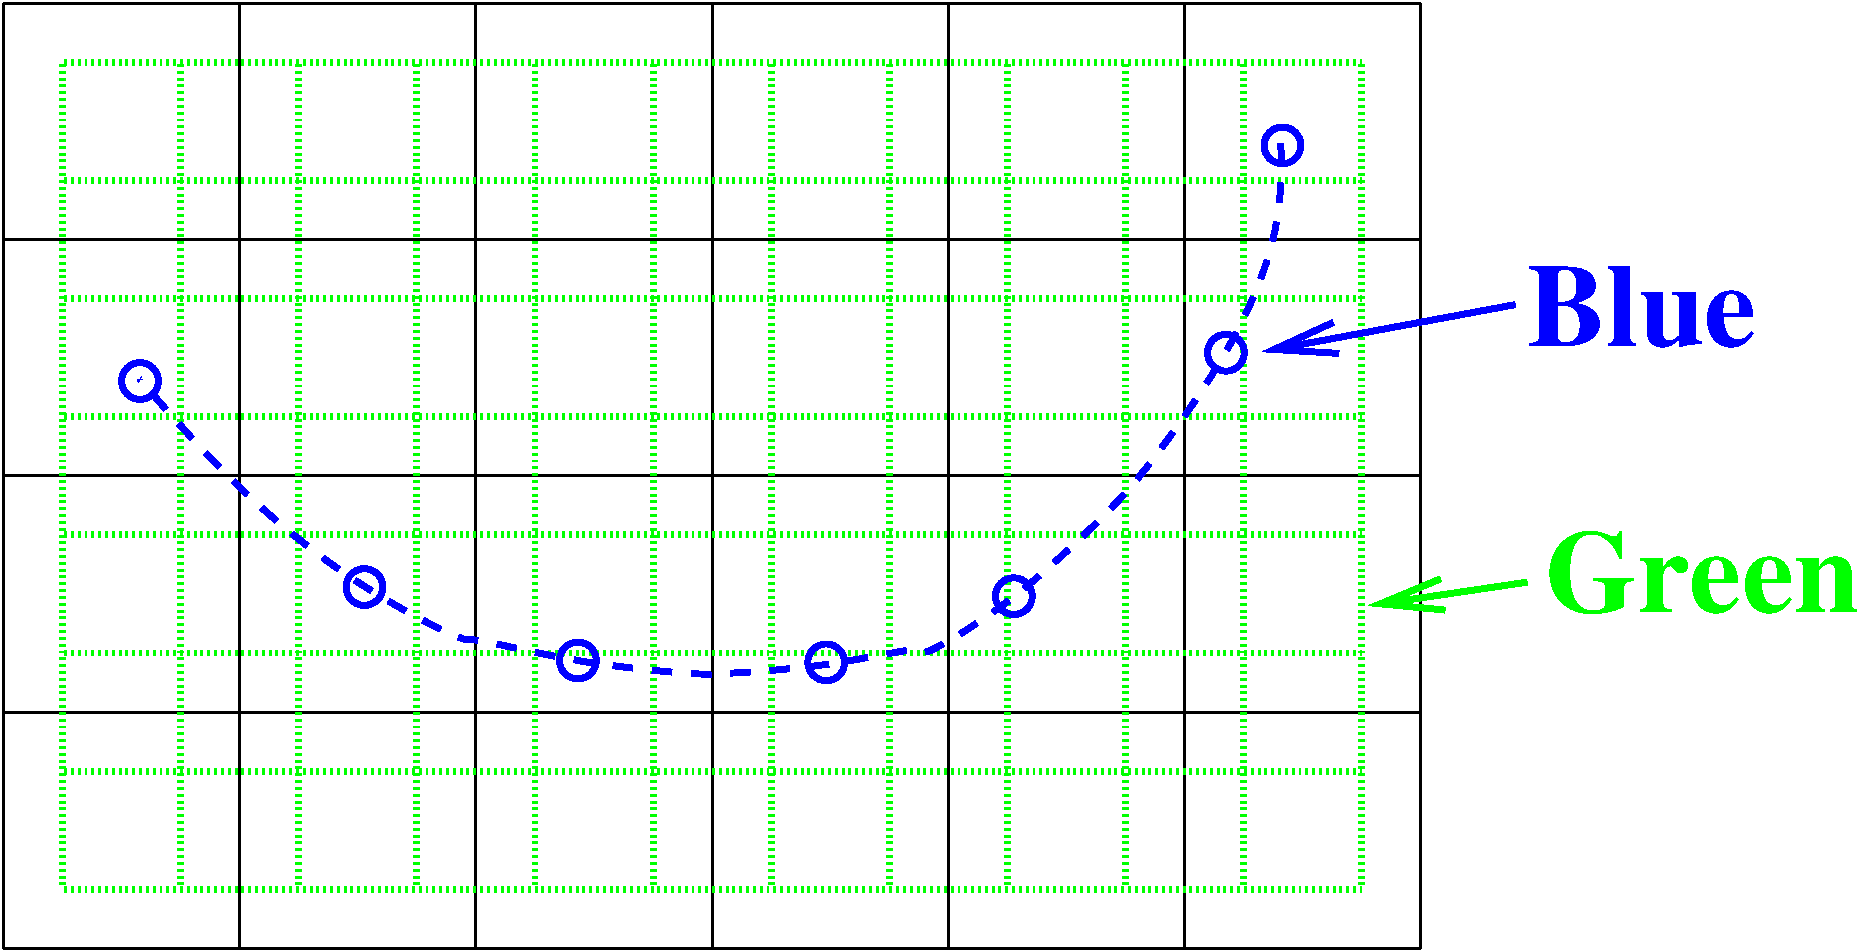
\includegraphics[width=.6\hsize]{interpolation/interpolation_types}
  \caption{The two different types of interpolation. Green (dotted):
    Interpolation to a new grid, output has same dimension as input,
    in this case 2D. Blue (dashed): Interpolation to a sequence of
    points, output is always 1D.}
  \label{fig:interpolation:types}
\end{figure}

There are two different types of interpolation in ARTS:
\begin{description}
\item[Green Interpolation:] Interpolation of a gridded field to a new
  grid.
\item[Blue Interpolation:] Interpolation of a gridded field to a
  sequence of positions.
\end{description}
Figure \ref{fig:interpolation:types} illustrates the different types
for a 2D example. 

The first step of an interpolation always consists in determining
where your new points are, relative to the original grid. You can do
this separately for each dimension. The positions have to be stored
somehow, which is described in the next section.



\levelb{Grid positions}
%-------------------------------------------------------------------------

A grid position specifies where an interpolation point is, relative
to the original grid. It consists of three parts, an \verb|Index| giving the
original grid index below the interpolation point, a \verb|Numeric|
giving the fractional distance to the next original grid point, and a
\verb|Numeric| giving 1 minus this number. Of course, the last element is
redundant. However, it is efficient to store this, since it is used
many times over. We store the two numerics in a plain C array of
dimension 2. (No need to use a fancy Array or Vector for this, since
the dimension is fixed.) So the structure is:

\begin{verbatim}
struct GridPos {
   Index   idx;      /*!< Original grid index below
                          interpolation point. */
   Numeric fd[2];    /*!< Fractional distance to next point
                          (0<=fd[0]<=1), fd[1] = 1-fd[0]. */ 
};
\end{verbatim}

For example, \verb|idx|=3 and \verb|fd|=0.5 means that this interpolation point is
half-way between index 3 and 4 of the original grid.  Note, that
`below' in the first paragraph means `with a lower index'. If the
original grid is sorted in descending order, the value at the grid
point below the interpolation point will be numerically higher than
the interpolation point.  In other words, grid positions and
fractional distances are defined relative to the order of the original
grid. Examples:

{\small
\begin{verbatim}
old grid = 2 3
new grid = 2.25
idx      = 0
fd[0]    = 0.25

old grid = 3 2
new grid = 2.25
idx      = 0
fd[0]    = 0.75
\end{verbatim}
}

Note that \verb|fd[0]| is different in the second case, because the old grid
is sorted in descending order. Note also that \verb|idx| is the same in
both cases.

Grid positions for a whole new grid are stored in an \verb|Array<GridPos>|
(called \verb|ArrayOfGridPos|). 

\levelb{Setting up grid position arrays}
%----------------------------------------------------------------------

There is only one function to set up grid position arrays:

{\small
\begin{verbatim}
void gridpos( ArrayOfGridPos& gp,
              ConstVectorView old_grid,
              ConstVectorView new_grid );
\end{verbatim}
}

\hspace{-\parindent}Some points to remember:
\begin{itemize}
\item As usual, the output \verb|gp| has to have the right dimension. 
  
\item The old grid has to be strictly sorted. It can be in ascending
  or descending order. But there must not be any duplicate values.
  Furthermore, the old grid must contain at least two points.
  
\item   The new grid does not have to be sorted, but the function will be
  faster if it is sorted or mostly sorted. It is ok if the new grid
  contains only one point.
  
\item   The beauty is, that this is all it needs to do also interpolation in
  higher dimensions: You just have to call gridpos for all the
  dimensions that you want to interpolate.
  
\item   Note also, that for this step you do not need the field itself at
  all!
\end{itemize}

\levelb{Interpolation weights}
%----------------------------------------------------------------------

As explained in the `Numerical Recipes'
\citep{numerical_recipes_C:97}, 2D bi-linear interpolation means, that
the interpolated value is a weighted average of the original field at
the four corner points of the grid square in which the interpolation
point is located. For simplicity, we label the four corner points
counterclockwise, starting from the lower left point (Figure
\ref{fig:interpolation:square}).  Then the interpolated value is given
by:
\begin{eqnarray}
  y(t,u)
  &=& (1-t)*(1-u)*y_1 \nonumber \\
  & & \mbox{} + t*(1-u)*y_2 \nonumber \\
  & & \mbox{} + t*u*y_3 \nonumber \\
  & & \mbox{} + (1-t)*u*y_4 \nonumber \\
  &=& w_1*y_1 + w_2*y_2 + w_3*y_3 + w_4*y_4
\label{eq:interpolation:weights}
\end{eqnarray}
where $t$ and $u$ are the fractional distances between the
corner points in the two dimensions, $y_i$ are the field values
at the corner points, and $w_i$ are the interpolation weights.

\begin{figure}
  \centering
  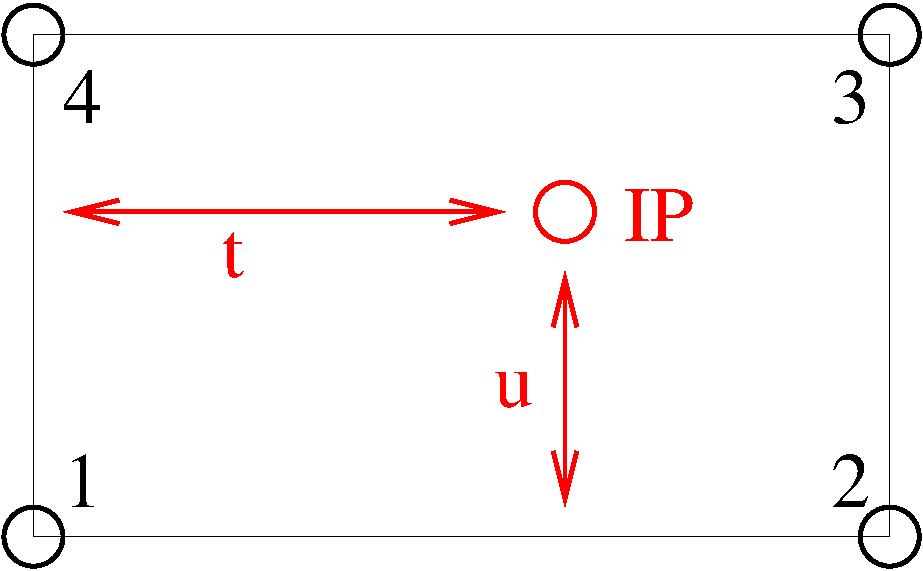
\includegraphics[width=.4\hsize]{interpolation/interpolation_square}
  \caption{The grid square for 2D interpolation. The numbers 1\ldots 4
    mark the corner points, IP is the interpolation point, $t$ and $u$
    are the fractional distances in the two dimensions.}
  \label{fig:interpolation:square}
\end{figure}

(By the way, I have discovered that this is exactly the result that
you get if you first interpolate linearly in one dimension, then in
the other. I was playing around with this a bit, but it is the more
efficient way to pre-calculate the $w_i$ and do all dimensions at once.

How many interpolation weights one needs for a multilinear
interpolation depends on the dimension of the interpolation: There are
exactly $2^n$ interpolation weights for an $n$ dimensional
interpolation.  These weights have have to be computed for each
interpolation point (each grid point of the new grid, if we do a
`green' type interpolation. Or each point in the sequence, if we do a
`blue' type interpolation).

This means, calculating the interpolation weights is not exactly
cheap, especially if one interpolates simultaneously in many
dimensions. On the other hand, one can save a lot by re-using the
weights.  Therefore, interpolation weights in ARTS are stored in a
tensor which has one more dimension than the output field. The last
dimension is for the weight, so this last dimension has the extent 4
in the 2D case, 8 in the 3D case, and so on (always $2^n$).

In the case of a `blue' type interpolation, the weights are
always stored in a matrix, since the output field is always 1D (a
vector). 

\levelb{Setting up interpolation weight tensors}
%----------------------------------------------------------------------

Interpolation weight tensors can be computed by a family of functions,
which are all called \verb|interpweights|. Which function is actually
used depends on the dimension of the input and output quantities. For
this step we still do not need the actual fields, just the grid
positions.

\levelc{Blue interpolation}

In this case the functions are:

{\small
\begin{verbatim}
void interpweights( MatrixView itw,
                    const ArrayOfGridPos& cgp );
void interpweights( MatrixView itw,
                    const ArrayOfGridPos& rgp,
                    const ArrayOfGridPos& cgp );
void interpweights( MatrixView itw,
                    const ArrayOfGridPos& pgp,
                    const ArrayOfGridPos& rgp,
                    const ArrayOfGridPos& cgp );
void interpweights( MatrixView itw,
                    const ArrayOfGridPos& vgp,
                    const ArrayOfGridPos& sgp,
                    const ArrayOfGridPos& bgp,
                    const ArrayOfGridPos& pgp,
                    const ArrayOfGridPos& rgp,
                    const ArrayOfGridPos& cgp );
\end{verbatim}
}

In all cases, the dimension of \verb|itw| must be consistent with the
given grid position arrays and the dimension of the interpolation
(last dimension $2^n$). Because the grid position arrays are
interpreted as defining a sequence of positions they must all have
the same length.

\levelc{Green interpolation}

In this case the functions are:

{\small
\begin{verbatim}
void interpweights( Tensor3View itw,
                    const ArrayOfGridPos& rgp,
                    const ArrayOfGridPos& cgp );
void interpweights( Tensor4View itw,
                    const ArrayOfGridPos& pgp,
                    const ArrayOfGridPos& rgp,
                    const ArrayOfGridPos& cgp );
void interpweights( Tensor5View itw,
                    const ArrayOfGridPos& bgp,
                    const ArrayOfGridPos& pgp,
                    const ArrayOfGridPos& rgp,
                    const ArrayOfGridPos& cgp );
void interpweights( Tensor6View itw,
                    const ArrayOfGridPos& sgp,
                    const ArrayOfGridPos& bgp,
                    const ArrayOfGridPos& pgp,
                    const ArrayOfGridPos& rgp,
                    const ArrayOfGridPos& cgp );
void interpweights( Tensor7View itw,
                    const ArrayOfGridPos& vgp,
                    const ArrayOfGridPos& sgp,
                    const ArrayOfGridPos& bgp,
                    const ArrayOfGridPos& pgp,
                    const ArrayOfGridPos& rgp,
                    const ArrayOfGridPos& cgp );
\end{verbatim}
}

In this case the grid position arrays are interpreted as defining the
grids for the interpolated field, therefore they can have different
lengths. Of course, \verb|itw| must be consistent with the length of
all the grid position arrays, and with the dimension of the
interpolation (last dimension $2^n$).

\levelb{The actual interpolation}
%----------------------------------------------------------------------

For this final step we need the grid positions, the
interpolation weights, and the actual fields. For each interpolated
value, the weights are applied to the appropriate original field values
and the sum is taken (see Equation
\ref{eq:interpolation:weights}). The \verb|interp| family of functions
performs this step.

\levelc{Blue interpolation}

{\small
\begin{verbatim}
void interp( VectorView            ia,
             ConstMatrixView       itw,
             ConstVectorView       a,    
             const ArrayOfGridPos& cgp);
void interp( VectorView            ia,
             ConstMatrixView       itw,
             ConstMatrixView       a,    
             const ArrayOfGridPos& rgp,
             const ArrayOfGridPos& cgp);
void interp( VectorView            ia,
             ConstMatrixView       itw,
             ConstTensor3View      a,    
             const ArrayOfGridPos& pgp,
             const ArrayOfGridPos& rgp,
             const ArrayOfGridPos& cgp);
void interp( VectorView            ia,
             ConstMatrixView       itw,
             ConstTensor4View      a,    
             const ArrayOfGridPos& bgp,
             const ArrayOfGridPos& pgp,
             const ArrayOfGridPos& rgp,
             const ArrayOfGridPos& cgp);
void interp( VectorView            ia,
             ConstMatrixView       itw,
             ConstTensor5View      a,    
             const ArrayOfGridPos& sgp,
             const ArrayOfGridPos& bgp,
             const ArrayOfGridPos& pgp,
             const ArrayOfGridPos& rgp,
             const ArrayOfGridPos& cgp);
void interp( VectorView            ia,
             ConstMatrixView       itw,
             ConstTensor6View      a,    
             const ArrayOfGridPos& vgp,
             const ArrayOfGridPos& sgp,
             const ArrayOfGridPos& bgp,
             const ArrayOfGridPos& pgp,
             const ArrayOfGridPos& rgp,
             const ArrayOfGridPos& cgp);
\end{verbatim}
}

\levelc{Green interpolation}

{\small
\begin{verbatim}
void interp( MatrixView            ia,
             ConstTensor3View      itw,
             ConstMatrixView       a,   
             const ArrayOfGridPos& rgp,
             const ArrayOfGridPos& cgp);
void interp( Tensor3View           ia,
             ConstTensor4View      itw,
             ConstTensor3View      a,   
             const ArrayOfGridPos& pgp,
             const ArrayOfGridPos& rgp,
             const ArrayOfGridPos& cgp);
void interp( Tensor4View           ia,
             ConstTensor5View      itw,
             ConstTensor4View      a,   
             const ArrayOfGridPos& bgp,
             const ArrayOfGridPos& pgp,
             const ArrayOfGridPos& rgp,
             const ArrayOfGridPos& cgp);
void interp( Tensor5View           ia,
             ConstTensor6View      itw,
             ConstTensor5View      a,   
             const ArrayOfGridPos& sgp,
             const ArrayOfGridPos& bgp,
             const ArrayOfGridPos& pgp,
             const ArrayOfGridPos& rgp,
             const ArrayOfGridPos& cgp);
void interp( Tensor6View           ia,
             ConstTensor7View      itw,
             ConstTensor6View      a,   
             const ArrayOfGridPos& vgp,
             const ArrayOfGridPos& sgp,
             const ArrayOfGridPos& bgp,
             const ArrayOfGridPos& pgp,
             const ArrayOfGridPos& rgp,
             const ArrayOfGridPos& cgp);
\end{verbatim}
}

\levelb{Examples}
%----------------------------------------------------------------------

\levelc{A simple example}

This example is contained in file \verb|test_interpolation.cc|.

{\small
\begin{verbatim}
void test05()
{
  cout << "Very simple interpolation case\n";

  Vector og(1,5,+1);            // 1, 2, 3, 4, 5
  Vector ng(2,5,0.25);          // 2.0, 2,25, 2.5, 2.75, 3.0

  cout << "Original grid:\n" << og << "\n";
  cout << "New grid:\n" << ng << "\n";

  // To store the grid positions:
  ArrayOfGridPos gp(ng.nelem());

  gridpos(gp,og,ng);
  cout << "Grid positions:\n" << gp;

  // To store interpolation weights:
  Matrix itw(gp.nelem(),2);
  interpweights(itw,gp);
    
  cout << "Interpolation weights:\n" << itw << "\n";

  // Original field:
  Vector of(og.nelem(),0);
  of[2] = 10;                   // 0, 0, 10, 0, 0

  cout << "Original field:\n" << of << "\n";

  // Interpolated field:
  Vector nf(ng.nelem());

  interp(nf, itw, of, gp);

  cout << "New field:\n" << nf << "\n";
}
\end{verbatim}
}

\hspace{-\parindent}Ok, maybe you think this is not so simple, but a
large part of the code is either setting up the example grids and
fields, or output. And here is how the output looks like:

{\small
\begin{verbatim}
Very simple interpolation case
Original grid:
  1   2   3   4   5
New grid:
  2 2.25 2.5 2.75   3
Grid positions:
   1 0    1
   1 0.25 0.75
   1 0.5  0.5
   1 0.75 0.25
   1 1    0
Interpolation weights:
  1   0
0.75 0.25
0.5 0.5
0.25 0.75
  0   1
Original field:
  0   0  10   0   0
New field:
  0 2.5   5 7.5  10
\end{verbatim}
}

\levelc{A more elaborate example}

What if you want to interpolate only some dimensions of a tensor,
while retaining others? --- You have to make a loop yourself, but it
is very easy. Below is an explicit example for a more complicated
interpolation case. (Green type interpolation of all pages of a
Tensor3.) This example is also contained in file
\verb|test_interpolation.cc|.

{\small
\begin{verbatim}
void test04()
{
  cout << "Green type interpolation of all "
       << "pages of a Tensor3\n";

  // The original Tensor is called a, the new one n. 

  // 10 pages, 20 rows, 30 columns, all grids are: 1,2,3
  Vector  a_pgrid(1,3,1), a_rgrid(1,3,1), a_cgrid(1,3,1); 
  Tensor3 a( a_pgrid.nelem(),
             a_rgrid.nelem(),
             a_cgrid.nelem() ); 
  a = 0;
  // Put some simple numbers in the middle of each page:
  a(0,1,1) = 10;
  a(1,1,1) = 20;
  a(2,1,1) = 30;

  // New row and column grids:
  // 1, 1.5, 2, 2.5, 3
  Vector  n_rgrid(1,5,.5), n_cgrid(1,5,.5); 
  Tensor3 n( a_pgrid.nelem(),
             n_rgrid.nelem(),
             n_cgrid.nelem() ); 

  // So, n has the same number of pages as a, 
  // but more rows and columns.

  // Get the grid position arrays:
  ArrayOfGridPos n_rgp(n_rgrid.nelem()); // For rows.
  ArrayOfGridPos n_cgp(n_cgrid.nelem()); // For columns.

  gridpos( n_rgp, a_rgrid, n_rgrid );
  gridpos( n_cgp, a_cgrid, n_cgrid );

  // Get the interpolation weights:
  Tensor3 itw( n_rgrid.nelem(), n_cgrid.nelem(), 4 );
  interpweights( itw, n_rgp, n_cgp );

  // Do a "green" interpolation for all pages of a:

  for ( Index i=0; i<a.npages(); ++i )
    {
      // Select the current page of both a and n:
      ConstMatrixView ap = a( i,
                              Range(joker), Range(joker) );
      MatrixView      np = n( i,
                              Range(joker), Range(joker) );

      // Do the interpolation:
      interp( np, itw, ap, n_rgp, n_cgp );

      // Note that this is efficient, because interpolation
      // weights and grid positions are re-used.
    }

  cout << "Original field:\n";
  for ( Index i=0; i<a.npages(); ++i )
      cout << "page " << i << ":\n"
           << a(i,Range(joker),Range(joker)) << "\n";

  cout << "Interpolated field:\n";
  for ( Index i=0; i<n.npages(); ++i )
      cout << "page " << i << ":\n"
           << n(i,Range(joker),Range(joker)) << "\n";
}
\end{verbatim}
}

\hspace{-\parindent}The output is:

{\small
\begin{verbatim}
Green type interpolation of all pages of a Tensor3
Original field:
page 0:
  0   0   0
  0  10   0
  0   0   0
page 1:
  0   0   0
  0  20   0
  0   0   0
page 2:
  0   0   0
  0  30   0
  0   0   0
Interpolated field:
page 0:
  0   0   0   0   0
  0 2.5   5 2.5   0
  0   5  10   5   0
  0 2.5   5 2.5   0
  0   0   0   0   0
page 1:
  0   0   0   0   0
  0   5  10   5   0
  0  10  20  10   0
  0   5  10   5   0
  0   0   0   0   0
page 2:
  0   0   0   0   0
  0 7.5  15 7.5   0
  0  15  30  15   0
  0 7.5  15 7.5   0
  0   0   0   0   0
\end{verbatim}
}

\levelb{Summary}
%----------------------------------------------------------------------

Now you probably understand better what was written at the very
beginning of this chapter, namely that doing an interpolation always
requires the chain of function calls:
\begin{enumerate}
\item \verb|gridpos| (one for each interpolation dimension)
\item \verb|interpweights|
\item \verb|interp|
\end{enumerate}
If you are interested in how the functions really work, look in file
\verb|interpolation.cc|. The documentation there is quite detailed.
When you are using interpolation, you should always give some thought
to whether you can re-use grid positions or even interpolation
weights. This can really save you a lot of computation time. For
example, if you want to interpolate several fields --- which are all
on the same grids --- to some position, you only have to compute the
weights once.


%%% Local Variables: 
%%% mode: latex 
%%% TeX-master: "uguide" 
%%% TeX-master: "uguide"
%%% End:


\chapter{Integration functions}
%--------------------------------------------------------------------------
\label{sec:integration}

\starthistory
  220802 & Created and written by Sreerekha T.R.\\
  220103 & Included mathematical description for implemented integration method(CE).\\
\stophistory

%
% Introduction
%
A radiative transfer model which takes into account the effect of
scattering involves integration of certain quantities over the angles
of observation.  For example from Section
\ref{sec:scattering:solution_rte} it is clear that computing  
scattering cross-section  and scattering integral term requires
integration over zenith and azimuth directions. There are a wide range of
methods that can be used for numerical integration. They can be used
depending on various factors starting from how accurate the result
should be to the behaviour of the function. The one which is
implemented in ARTS is the trapezoidal integration method. 


\section{Implementation files}
%-------------------------------------------------------------------------
\label{sec:integration:files}

The integration functions can be found in the files:
\begin{itemize}
\item \artsstyle{math\_funcs.h}
\item \artsstyle{math\_funcs.cc}
\end{itemize}
The implementation function \artsstyle {AngIntegrate\_trapezoid}is
discussed in the second file. 

\section{Trapezoidal Integration}
%------------------------------------------------------------------------
\label{sec:integration:trapezoidal}

Trapezoidal Integration method comes under the Newton-Cotes formulas
where integration of a function is approximated by the area under the
curve described by the function.  Trapezoidal integration assumes that
the area under the curve is trapezoid.  

Trapezoidal rule : 
\begin{eqnarray}
\label{eq:trapezoidal_rule}
{\int_{x_1}^{x_2} f(x)dx}  = \frac{1}{2} h (f_1 + f_2) + O(h^3 f^{''})
\end{eqnarray}
This is a two-point formula ($x_1$ and $x_2$).  It is exact for
polynomials upto and including degree 1, i.e., f(x) = x. $O(h^3
f^{''})$ signifies how far is the true answer from the estimate. 

If we use eq. \ref{eq:trapezoidal_rule} $N - 1$ times, to do the
integration in the intervals $(x_1, x_2)$,  $(x_2, x_3)$, ...,
$(x_{N-1}, x_N)$, and then add the results, we obtain extended formula
for the integral from $x_1$ to $x_N$.

Extended Trapezoidal rule :
\begin{eqnarray}
\label{eq:ext_trapezoidal_rule}
{\int_{x_1}^{x_N} f(x)dx}  = \frac{1}{2} h \left [f_1 + 2(f_2 + f_3 +
... +f_{N-1})+f_N \right] + O\left [ \frac {(b-a)^3 f^{''}}{N^2} \right]
\end{eqnarray}

The last term tells how much the error will be decreased by taking
more number of steps. 

\section{Solid Angle Integration}
%------------------------------------------------------------------------
\label{sec:integration:solid_angle}
In our scattering problem, we are often encountered with a double integration
of functions over zenith and azimuth angles (see Chapter
\ref{sec:scattering}).  One way to achieve
double integration is to use repeated
one-dimensional trapezoidal integration.  This is effective of course
only if the boundary is simple and the function is very smooth.  If
the function is strongly peaked and if know where it occurs, integral
should be broken into smaller regions so that the 
integrand is smooth in each.  Another thing is to take into account
the symmetry of the function as well as the boundary. For example in
our case, if the radiation is symmetric about the azimuth, the
integration in that direction returns constant value of $2 \pi$ and we
need to do only integration over zenith directions.  

The general form of a solid angle integration is
\begin{equation}
  \label{eq:solid_int}
S = \int_{4\pi} f(\omega) \DiffD\omega
\end{equation}
In spherical coordinates we can write:
\begin{equation}
  \label{eq:sol_int_sph}
 S = \int_0^\pi \int_0^{2\pi} f(\theta,\phi) \sin\theta \quad\DiffD\theta\DiffD\phi
\end{equation}
A double integration can be splitted into two single integrations:
\begin{eqnarray}
 S &=& \int_0^\pi \left(\int_0^{2\pi}  f(\theta,\phi) \sin\theta \DiffD\phi \right) \DiffD\theta \\
 &=& \int_0^\pi g(\theta) \DiffD\theta
\end{eqnarray}
If we have to integrate a vector, we can apply this method componentwise.

To solve the integral numerically we discretize $\theta$ and $\phi$ and obtain two angular grids ( $[\theta_0, \theta_1, \cdots, \theta_n]$  and $[\phi_0, \phi_1, \cdots, \phi_m]$). 
Then we can first calculate $g(\theta_j)$ for all $\theta_j$ unsing the trapezoidal method.
\begin{equation}
  g(\theta_j) = \sum_{i=1}^m \sin\theta_j \frac{f(\theta_j, \phi_i) + f(\theta_j, \phi_{i+1})}{2} \cdot (\phi_{i+1} - \phi_i)  
\end{equation}
The final step is to sum up all $g(\theta_j)$, again applying the trapezoidal method.
\begin{equation}
  S = \sum_{j=1}^n \frac{g(\theta_j) + g(\theta_{j+1})}{2} \cdot  (\theta_{j+1} - \theta_j)  
\end{equation}

If the radiation is symmetric about the azimuth we just calculate:
\begin{equation}
  S_{sym} = 2\pi \int_0^{\pi} f(\theta) \sin(\theta) \DiffD \theta 
\end{equation}
Unsing the trapezoidal method this can be written as:
\begin{equation}
  S_{sym} =  2\pi \sum_{j=1}^n \frac{h(\theta_j) + h(\theta_{j+1})}{2} \cdot  (\theta_{j+1} - \theta_j)  
\end{equation}
where $h(\theta) = \sin\theta\cdot f(\theta)$.
 
\vspace{2ex}



The function  \artsstyle{AngIntegrate\_trapezoid} takes as input the integrand and the angles over which
the integration has to be done. For example in this case it can be the
zenith and azimuth angle
grid.
\begin{verbatim}  
Numeric AngIntegrate_trapezoid(MatrixView Integrand,
                               ConstVectorView za_grid,
                               ConstVectorView aa_grid)
\end{verbatim}
The integrand has the same number of rows as zenith angle grid
and columns as azimuth angle grid.  The inner loop does trapezoidal
integration of the integrand over all azimuth angles and the result is
stored in a Vector  res1[i]. Note that the integrand at every point
has to be multiplied with \artsstyle {sin (za\_grid[i] * DEG2RAD)}
since we are integrating over solid angles.  The outer loop 
does an integration of res1[i] over all zentih angles.  The result of
this is returned back to the calling function.  


%%% Local Variables: 
%%% mode: latex
%%% TeX-master: t
%%% End: 

\levela{Linear Algebra functions}
%--------------------------------------------------------------------------
\label{sec:lin_alg}

\starthistory
  020502 & Created and written by Claudia Emde.\\
\stophistory

%
% Introduction
%

Solving the vector radiative transfer equation requires the
computation of linear equation systems and the matrix
exponential. This section describes the functions which are implemented
in ARTS and it gives instructions how these functions can be used, also
for other purposes than the radiative transfer calculations.

\levelb{Implementation files}
%-------------------------------------------------------------------------
\label{sec:lin_alg:files}

All the functions described below can be found in the files:
\begin{itemize}
\item \artsstyle{lin\_alg.h}
\item \artsstyle{lin\_alg.cc}
\end{itemize}
The template class \artsstyle{Array} and the classes \artsstyle{Matrix} and
\artsstyle{Vector} are used, therefore the linear algebra functions require
the files:
\begin{itemize}
\item \artsstyle{matpackI.h}
\item \artsstyle{make\_vector.h}
\item \artsstyle{array.h}
\item \artsstyle{matpackI.cc}
\item \artsstyle{make\_vector.cc}
\item \artsstyle{array.cc}
\end{itemize}
Furthermore logical functions contained in
\begin{itemize}
\item \artsstyle{logic.h}
\item \artsstyle{logic.cc}
\end{itemize}
are used to check the dimensions of input matrices for various functions.


\levelb{Linear Equation Systems}
%------------------------------------------------------------------------
\label{sec:lin_alg:lineqsys}


For solving a set of linear equations 
\begin{eqnarray}
\label{eq:lin_equ_sys}
{\bf A} {\bf x} = {\bf b}
\end{eqnarray}
the LU decomposition method is implemented.A slightly modified version
of the algorithm described in
[\cite{numerical_recipes_C:97}] is used here. An alternative method
is the Gauss-Jordan elimination, but this method is three times
slower than the LU decomposition method
[\cite{numerical_recipes_C:97}, p.36]. The LU decomposition method
reqires two functions, \artsstyle{ludcmp} and \artsstyle{lubacksub},
which will be decribed below.
\vspace{0.5cm}\\
The following example for a three dimensional equation sytem 
demonstrates how to solve a linear
equation sytem of the type
(\ref{eq:lin_equ_sys}):
\begin{itemize}
\item Create matrix A, vector b: \\
  \artsstyle{A = Matrix(3,3);} \\
  \artsstyle{A(1,1) = 4;}\\
  \artsstyle{A(2,1) = 3;}\\
  $\cdots$\\
  \artsstyle{b = Vector(3);}\\
  \artsstyle{b(1) = 7;}\\
  $\cdots$
\item Initialize solution vector x and two other variables needed for
  storing intermediate results:\\
  \artsstyle{x = Vector(3);}\\
  \artsstyle{LU = Matrix(3,3);}\\
  \artsstyle{indx = ArrayOfIndex(3);}
\item Call LU decomposition function (see Section \ref{sec:lin_alg:lu_decomp}): \\
  \artsstyle{ludcmp(LU, indx, A);}
\item Call LU backsubstitution function (see Section \ref{sec:lin_alg:backsub}): \\
  \artsstyle{lubacksub(x, LU, b, indx);}
\item Print the solution vector:\\
  \artsstyle{cout << x;}
\end{itemize}

\levelc{LU Decomposition}
%------------------------------------------------------------------------
\label{sec:lin_alg:lu_decomp}

A LU decomposition is a procedure for decomposing a square matrix {\bf
  A} with
dimension $n$ into a product of a lower triangular matrix {\bf L} (has
elements only on the diagonal elements and below) and
an upper triangular matrix {\bf U} (has elements only on the diagonal
and above):
\begin{equation}
  \label{eq:lu_decomp}
  {\bf L}\cdot{\bf U} ={\bf A} 
\end{equation}
For a 3 x 3 matrix equation \ref{eq:lu_decomp} would look like this: 
\[ \left(
  \begin{array}{ccc}
    l_{11} & 0 & 0 \\
    l_{21} & l_{22} & 0 \\
    l_{31} & l_{32} & l_{33}
    \end{array} \right)
\cdot
\left(
  \begin{array}{ccc}
    u{11} & u_{12} & u_{13} \\
    0 & u_{22} & u_{23}\\
    0 & 0 & u_{33}
    \end{array} \right)
=
\left(
  \begin{array}{ccc}
    a_{11} & a_{12} & a_{13} \\
    a_{21} & a_{22} & a_{23} \\
    a_{31} & a_{32} & a_{33}
    \end{array} \right)
\]
The decomposition can be used to rewrite the linear set of equations
(\ref{eq:lin_equ_sys}) in the following way:
\begin{eqnarray}
  {\bf A}\cdot{\bf x} = ({\bf L}\cdot{\bf U})\cdot{\bf x} = {\bf
    L}\cdot({\bf U}\cdot{\bf x}) = {\bf b}
\end{eqnarray}
First 
\begin{equation}
  {\bf L} \cdot{\bf y} = {\bf b}
\end{equation}
is solved for the vector ${\bf y}$ which can be done by
forward substitution (see section \ref{sec:lin_alg:backsub}). Then 
\begin{equation}
  {\bf U} \cdot{\bf x} = {\bf y}
\end{equation}
is solved again by backsubstitution. 
The advantage in breaking up one linear set into two successive ones
is that the solution of a triangular set of equations is quite trivial.

The function \artsstyle{ludcmp} requires a square matrix of arbitrary
dimension $n$ as input and performs the LU decomposition. It returns one
matrix which contains both matrices, ${\bf L}$ and ${\bf U}$. 
For the lower triangular matrix  ${\bf L}$ the diagonal elements 
are chosen to be 1, then the other elements of ${\bf L}$ and ${\bf U}$
are determined. This is possible, as the LU decomposition is an under
determined equation sytem with $n^2$ equations for $n^2+n$ unknowns. 
The output matrix does not include the diagonal of ${\bf L}$, in the
three-dimensional case it has the following elements:
\[ \left(
  \begin{array}{ccc}
    u_{11} & u_{12} & u_{13} \\
    l_{21} & u_{22} & u_{23} \\
    l_{31} & l_{32} & u_{33}
    \end{array} \right)
\]
This special arrangement of the LU decomposition is named {\sl
Crout's algorithm} and a matrix arranged in this form is named {\sl
Crout matrix} in this context.
  

Another output variable of the function \artsstyle{ludcmp} is an index
vector which contains information about pivoting which is absolutely
essential for the stability of
Crout's algorithm. Here partial pivoting,
i.e. interchange of rows is implemented. That means that not {\bf A} is
decomposed into $LU$-form but a rowwise permutation of {\bf A}. If the
index vector contains for example the elements $(2,1,0)$ the first and
the last row of a three dimensional matrix would be exchanged.


\levelc{Forward- and Backsubstitution}
%---------------------------------------------------------------
\label{sec:lin_alg:backsub}
An equation system of the form
\[ 
\left(
  \begin{array}{ccc}
    a{11} & a_{12} & a_{13} \\
    0 & a_{22} & a_{23}\\
    0 & 0 & a_{33}
    \end{array} \right)
\cdot
\left(
  \begin{array}{c}
    x_1\\x_2\\x_3
 \end{array} \right)
=
\left(
  \begin{array}{c}
    b_1\\b_2\\b_3
 \end{array} \right)
\]
can be solved very easy. The last element, here $x_3$, is already isolated,
namely
\begin{eqnarray}
  x_3 = b_3/a_{33}
\end{eqnarray}
As $x_3$ is known $x_2$ can be calculated using the second row of the
eqautions. Then, finally, $x_1$ can be calculated as well using the
first row. This procedure
is called backsubtitution. The same
method  applied for an equation system including a
lower triangular matrix is named forward substitution.   

The function \artsstyle{lubacksub} does forward and backward
substitution to solve the equation system described in
\ref{sec:lin_alg:lu_decomp}. As input it requires the output variables of
\artsstyle{ludcmp} which are the {\sl Crout matrix} and the index
vector. Output of the function is the solution vector ${\bf x}$ to the
equation system.


\levelc{More Applications of the LU Decomposition}
%-------------------------------------------------------------------
\label{lu_applications}

\begin{itemize}
\item Inverse of a matrix:\\
  To compute $(\bf K)^{-1}\cdot{\bf b}$, which is a part of the
solution to the vector radiative transfer equation (\ref{eq:scattering:RTE}) the LU
decomposition method can be used. The following equations show, that
the problem is equivalent to  solving a linear equation system of the type
\ref{eq:lin_equ_sys}.
\begin{eqnarray}
  {\bf K}^{-1}\cdot{\bf b} &=& {\bf x}\\
\Leftrightarrow \qquad  {\bf K}\cdot{\bf x} &=& {\bf b}
\end{eqnarray}

\item To solve the equation system
  \begin{eqnarray}
    {\bf A}\cdot{\bf X} &=& {\bf B}
  \end{eqnarray}
where {\bf A}, {\bf B} and  {\bf X} are matrices of dimension
$n$, the LU decomposition functions can be applied as well. Assume
that {\bf A} and {\bf B} are known and you want to solve for {\bf
 X}.
First you should do a LU decomposition of  {\bf A} and then
backsubstitute with the columns of B and you get the columns of {\bf
  X} as solution vectors.

\end{itemize}

\levelb{Matrix Exponential Function}
%----------------------------------------------------------------
\label{sec:lin_alg:mat_exp}

A very important function for solving differential equations is the
matrix exponential:
\begin{eqnarray}
  \label{eq:mat_exp}
  e^{{\bf A}s} = \sum_{k=0}^\infty{\frac{({\bf A} s)^k}{k!}}
\end{eqnarray}
In principle it could be computed using the Taylor power series but 
 this method is not efficient. {\sc Moler} and {\sc Van
  Loan} have shown for the simple example [\cite{Moler_Loan:79}]
\[ {\bf A} =
\left(
  \begin{array}{cc}
    -49 & 24\\
    -64 & 31
    \end{array} \right) \]
that convergence is obtained not until 59 terms. And if a relative
accuracy of only 10$^{-5}$ is taken, the method even leads to a wrong
result due to rounding errors.

\levelc{Pad\'e Approximation}
%----------------------------------------------------------------------
\label{sec:pade_approximation}

One of the better algorithms for computing the matrix exponential is
the Pad\'e approximation which is also shortly described in
[\cite{Moler_Loan:79}] and outlined in the book ``Matrix
Computations'' by \cite{Golub_Loan:91}. 
The method uses perturbation theorie as well as the so called Pad\'e
functions. It is possible to derive an algorithm which calculates
\begin{eqnarray}
  {\bf F} = e^{{\bf A}+{\bf E}} 
\end{eqnarray}
where 
\begin{eqnarray}
  \|{\bf E}\|_\infty \le \delta \|{\bf A}\| .
\end{eqnarray}
The accuracy of the computation given by $\delta$ can be chosen. 
The parameter q has to be the smallest non-negative integer such that
$\epsilon(q,q)\le\delta$ where
\begin{eqnarray}
  \epsilon(p,q) = 2^{3-(p+q)}\frac{p!q!}{(p+q)!(p+q+1)!}.
\end{eqnarray}
The following table shows values of epsilon for
different values of q.
\vspace{0.5cm}\\
\begin{tabular}[h]{|r|r|}
 \hline
q & $\epsilon$(q,q) \\ \hline
1 & 0.1667\\
2 & 6.9444 $\cdot$ 10$^{-4}$ \\
3 & 1.2401 $\cdot$ 10$^{-6}$ \\
4 & 1.2302 $\cdot$ 10$^{-9}$ \\
5 & 7.7667 $\cdot$ 10$^{-13}$ \\
6 & 3.3945 $\cdot$ 10$^{-16}$ \\ 
\hline
\end{tabular}
\vspace{0.5cm}\\
The algorithm is implemented in the function \artsstyle{matrix\_exp}. Input
to this function is the matrix ${\bf A}$ and the parameter $q$. As output
it gives the matrix ${\bf F}$ which is defined above.\\
The following example shows how to use the \artsstyle{matrix\_exp} function:
\begin{itemize}
\item Initialize {\bf A} and assign values:\\
  \artsstyle{Matrix A(3,3);}\\
  \artsstyle{A(1,1) = 45;}\\
  \artsstyle{A(1,2) = 3;}\\
$\cdots$ 
\item Initialize {\bf F}:\\
  \artsstyle{Matrix F(3,3);}
\item Give a paramater for the accuracy:\\
  \artsstyle{Index q=6;}
\item Call the matrix exponential function:\\
  \artsstyle{matrix\_exp(F,A,q);}
\item Print the result: \\
  \artsstyle{cout << "exp(A) = " << F;}
\end{itemize}






%%% Local Variables: 
%%% mode: latex
%%% TeX-master: t
%%% End: 

%
\part{Theoretical background}
\graphicspath{{Figs/rte_theory/}}

%Inverse Wave Impendance
\newcommand{\ColVctTwo}[2]{\left[
    \begin{array}{c} #1\\ #2
    \end{array} \right] }

\newcommand{\ColVctFour}[4]{\left[
    \begin{array}{c} #1\\ #2 \\ #3 \\ #4
    \end{array} \right] }

\chapter{Basic radiative transfer theory}
 \label{sec:rte_theory}


\starthistory
  050224 & Copied chapter 1 from Claudia Emde's phd-thesis. \\
  030305 & Copied from a compendium written by Patrick Eriksson.
\stophistory


 When dealing with atmospheric radiation a division can be made
 between two different wavelength ranges where the limit is found
 around 5 $\mu$m, i.e. one range consists of the near IR, visible and UV
 regions while the second range covers thermal and far IR and
 microwaves. The first reason to this division is the principal
 sources to the radiation in the two ranges, for wavelengths shorter
 than 5 $\mu$m the solar radiation is dominating while at longer
 wavelengths the thermal emission from the surface and the atmosphere
 is more important. A second reason is the importance of scattering
 but here it is impossible to give a fixed limit. Clouds are important
 scattering objects for most frequencies but at cloud free conditions
 scattering can in many cases be neglected for wavelengths $>$ 5 $\mu$m. If
 the atmosphere can be assumed to be in local thermodynamic
 equilibrium the radiative transfer can be simplified considerably,
 and this is a valid assumption for the IR region and microwaves but
 not for e.g. UV frequencies.
 
 The radiative transfer in the atmosphere must be adequately described
 in many situations, as when estimating rates of photochemical
 reactions, calculating radiative forcing in the atmosphere or
 evaluating an remote sensing observation. It is not totally
 straightforward to quantify the radiative transfer with good accuracy
 because the calculations can be very computationally demanding and
 many of the parameters needed are hard to determine. For example,
 situations when a great number of transitions or multiple scattering
 must be considered will cause long calculations while as a rule
 scattering is problematic to model because the shape and size
 distribution of the scattering particles are highly variable
 quantities.  

 This chapter introduces the theoretical background which is essential
 to develop a radiative transfer model including scattering. The theory
 is based on concepts of electrodynamics, starting from the Maxwell
 equations.  An elementary book for electrodynamics is written by
 \citet{jackson98:_class}.  For optics and scattering of radiation by
 small particles the reader may refer for instance to
 \citet{hulst57:_light_scatt_small} and \citet{bohren:98}. The notation
 used in this chapter is mostly adapted from the book ``Scattering,
 Absorption, and Emission of Light by Small Particles'' by
 \citet{Mishchenko:02}. Several lengthy derivations of formulas, which
 are not shown in detail here, can also be found in this book. The
 purpose of this chapter is to provide definitions and give ideas, how
 these definitions can be derived using principles of electromagnetic
 theory. For the derivation of the radiative transfer equation an
 outline of the traditional phenomenological approach is given.
 
 \section{Basic definitions}
 \label{sec:rtetheory:theory_basics}
 
 From the Maxwell equations one can derive the formula for the
electromagnetic field vector $\VctStl{E}$ of a plane electromagnetic
wave propagating in a homogeneous medium without sources:
\begin{equation}
  \VctStl{E}(\VctStl{r}, t) =
  \VctStl{E}_0
  \exp\left(-\frac{\omega}{c} m_{\mathrm{I}} \hat{\PDir} \cdot \VctStl{r}\right)
  \exp\left(i \frac{\omega}{c} m_{\mathrm{R}} \hat{\PDir} \cdot \VctStl{r}  - i \omega t \right),
\end{equation}
where $\VctStl{E}_0$ is the amplitude of the electromagnetic wave in
vacuum, $c$ is the speed of light in vacuum, $\omega$ is the angular
frequency, $\VctStl{r}$ is the position vector and $\hat{\PDir}$
is a real unit vector in the direction of propagation. The complex
refractive index $m$ is
\begin{equation}
  m = m_{\mathrm{R}}+ i m_{\mathrm{I}} = c \sqrt{\epsilon \mu},
\end{equation}
where $m_{\mathrm{R}}$ is the non-negative real part and $m_{\mathrm{I}}$ is the non-negative imaginary part. Furthermore $\mu$ is the
permeability of the medium and $\epsilon$ the permittivity.  For a
vacuum, $m = m_{\mathrm{R}} = 1$.  The imaginary part of the refractive
index, if it is non-zero, determines the decay of the amplitude of the
wave as it propagates through the medium, which is thus absorbing.
The real part determines the phase velocity $v = c/m_{\mathrm{R}}$.
The time-averaged Poynting vector $\VctStl{P}(\VctStl{r})$, which describes the
flow of electromagnetic energy, is defined as
\begin{equation}
   \VctStl{P}(\VctStl{r}) =
     \frac{1}{2} \Re \bigl(\EnsAvr{\VctStl{E}(\VctStl{r})} \times
     \EnsAvr{\VctStl{H}^*(\VctStl{r})}\bigr),
\end{equation}
where $\VctStl{H}$ is the magnetic field vector and the $*$ denotes the
complex conjugate. The Poynting vector for a homogeneous wave is given
by
\begin{equation}
\label{eq:rtetheory:Poynting_vec}
  \EnsAvr{\VctStl{P}(\VctStl{r})} =
   \frac{1}{2}\Re \left( \sqrt{\frac{\epsilon}{\mu}} \right)
   \Abs{\VctStl{E}_0}^2
   \exp\left(-2\frac{\omega}{c} m_{\mathrm{I}} \hat{\PDir} \cdot
     \VctStl{r}\right) \hat{\PDir}.
\end{equation}
Equation \ref{eq:rtetheory:Poynting_vec} shows that the energy flows in the
direction of propagation and its absolute value $I(\VctStl{r}) =
\Abs{\EnsAvr{\VctStl{P}(\VctStl{r})}}$, which is usually called
intensity (or irradiance), is exponentially attenuated. Rewriting
Equation \ref{eq:rtetheory:Poynting_vec} gives
\begin{equation}
  I(\VctStl{r}) = I_0 \exp(-\alpha^p \hat{\PDir} \cdot \VctStl{r}),
\end{equation}
where $I_0$ is the intensity for $\VctStl{r} = \VctStl{0}$. The absorption
coefficient $\alpha^p$ is
\begin{equation}
  \alpha^p =
  2 \frac{\omega}{c} m_{\mathrm{I}} =
    \frac{4\pi m_{\mathrm{I}}}{\lambda} =
    \frac{4\pi m_{\mathrm{I}}\nu}{c},
\end{equation}
where $\lambda$ is the free-space wavelength and $\nu$ the frequency.
Intensity has the dimension of monochromatic flux
[$\mathrm{energy}/(\mathrm{area}\times\mathrm{time})$].
  

\section[The Stokes parameters]{The Stokes parameters}
\label{sec:rtetheory:Stokes_components}
  

Sensors usually do not measure directly the electric and the magnetic
fields associated with a beam of radiation. They measure quantities
that are time averages of real-valued linear combinations of products
of field vector components and have the dimension of intensity.
Examples of such observable quantities are the Stokes parameters.
Figure \ref{fig:RT_theory_coordinates} shows the coordinate system used
to describe the direction of propagation $\hat{\PDir}$ and the
polarization state of a plane electromagnetic wave.
\begin{figure}[t]
 \begin{center}
   \includegraphics*[width=0.6\hsize]{coordinate_system}
   \caption{Coordinate system to describe the direction of propagation and the polarization state of a plane electromagnetic wave (adapted from Mishchenko).}
  \label{fig:RT_theory_coordinates}  
 \end{center}
\end{figure}
The unit vector $\hat{\PDir}$ can equivalently be described by a
couplet $(\ZntAng, \AzmAng)$, where ${\ZntAng \in [0,\pi]}$ is the polar
(zenith) angle and $\AzmAng \in [0,2\pi)$ is the azimuth angle. The
electric field at the observation point is given by $\VctStl{E} =
\VctStl{E}_\ZntAng + \VctStl{E}_\AzmAng$, where $ \VctStl{E}_\ZntAng$ and
$\VctStl{E}_\AzmAng$ are the $\ZntAng$- and $\AzmAng$-components of the
electric field vector.  $\VctStl{E}_\ZntAng$ lies in the meridional
plane, which is the plane through $\hat{\PDir}$ and the $z$-axis, and
$\VctStl{E}_\AzmAng$ is perpendicular to this plane.
The Stokes parameters are defined as linear combinations of products
of the amplitudes $\VctStl{E}_\ZntAng$ and  $\VctStl{E}_\AzmAng$ which
form the $4\times1$ column vector \StoVec,
which is known as the Stokes vector.  Since the Stokes parameters are
real-valued and have the dimension of intensity, they can be measured
directly with suitable instruments. The Stokes parameters are a
complete set of quantities needed to characterize a plane
electromagnetic wave. They carry information of the complex amplitudes
and the phase difference.  The first Stokes parameter $I$ is the
intensity and the other components $Q$, $U$ and $V$ describe the
polarization state of the wave. For a detailed definition of the
Stokes parameters and how they can be measured refer to
Section \ref{sec:polarization}.

\section[Single particle scattering]{Scattering, absorption and thermal emission by a single particle}
\label{sec:rtetheory:theory_single_part}

A parallel monochromatic beam of electromagnetic radiation propagates
in vacuum without any change in its intensity or polarization state. A
small particle, which is interposed into the beam, can cause several
effects:
\begin{description}
\item[Absorption:] The particle converts some of the energy
  contained in the beam into other forms of energy.
\item[Elastic scattering:] Part of the incident energy is
  extracted from the beam and scattered into all spatial directions at
  the frequency of the incident beam. Scattering can change the
  polarization state of the radiation.
\item[Extinction:] The energy of the incident beam is reduced by
  an amount equal to the sum of absorption and scattering.
\item[Dichroism:] The change of the polarization state of the beam
  as it passes a particle.
\item[Thermal emission:] If the temperature of the particle is
  non-zero, the particle emits radiation in all directions over a
  large frequency range.
\end{description}
The beam is an oscillating plane magnetic wave, whereas the particle
can be described as an aggregation of a large number of discrete
elementary electric charges. The incident wave excites the charges to
oscillate with the same frequency and thereby radiate secondary
electromagnetic waves. The superposition of these waves gives the
total elastically scattered field.

One can also describe the particle as an object with a refractive
index different from that of the surrounding medium. The presence of
such an object changes the electromagnetic field that would otherwise
exist in an unbounded homogeneous space. The difference of the total
field in the presence of the object can be thought of as the field
\emph{scattered} by the object. The angular distribution and the
polarization of the scattered field depend on the characteristics of
the incident field as well as on the properties of the object as its
size relative to the wavelength and its shape, composition and
orientation.

\subsection{Definition of the amplitude matrix}
\label{sec:rtetheory:amp_mat}

For the derivation of a relation between the incident and the
scattered electric field we consider a finite scattering object in the
form of a single body or a fixed aggregate embedded in an infinite
homogeneous, isotropic and non-absorbing medium. We assume that the
individual bodies forming the scattering object are sufficiently large
that they can be characterized by optical constants appropriate to
bulk matter, not to optical constants appropriate for single atoms or
molecules. Solving the Maxwell equations for the internal volume,
which is the interior of the scattering object, and the external
volume one can derive a formula, which expresses the total electric
field everywhere in space in terms of the incident field and the field
inside the scattering object. Applying the far field approximation
gives a relation between incident and scattered field, which is that
of a spherical wave.  The amplitude matrix
$\MtrStl{S}(\hat{\PDir}^{\sca},\hat{\PDir}^{\inc})$ includes this relation:
\begin{equation}
  \label{eq:rtetheory:amplitude_matrix}
  \ColVctTwo{E_\ZntAng^{\sca}(r\hat{\PDir}^{\sca})}%
         {E_\AzmAng^{\sca}(r\hat{\PDir}^{\sca})}
         = \frac{e^{ikr}}{r}\MtrStl{S}(\hat{\PDir}^{\sca},\hat{\PDir}^{\inc}) 
 \ColVctTwo{E_{0\ZntAng}^{\inc}}%
         {E_{0\AzmAng}^{\inc}}.
\end{equation}
The amplitude matrix depends on the directions of incident
$\hat{\PDir}^{\inc}$ and scattering $\hat{\PDir}^{\sca}$ as well as on size,
morphology, composition, and orientation of the scattering object with
respect to the coordinate system. The distance between the origin and
the observation point is denoted by $r$ and the wave number of the
external volume is denoted by $k$.

The amplitude matrix provides a complete description of the scattering
pattern in the far field zone. The amplitude matrix explicitly depends
on $\AzmAng^{\inc}$ and $\AzmAng^{\sca}$ even when $\ZntAng^{\inc}$ and/or
$\ZntAng^{\sca}$ equal 0 or $\pi$.

\subsection{Phase matrix}
\label{sec:rtetheory:pha_mat}

The phase matrix \PhaMat\ describes the transformation of the Stokes
vector of the incident wave into that of the scattered wave for
scattering directions away from the incidence direction
$(\hat{\PDir}^{\sca}\neq\hat{\PDir}^{\inc})$,
\begin{equation}
  \label{eq:rtetheory:phase_matrix}
  \StoVec^{\sca}(r \hat{\PDir}^{\sca}) =
    \frac{1}{r^2}\PhaMat(\hat{\PDir}^{\sca},\hat{\PDir}^{\inc}) \StoVec^{\inc}.
\end{equation}
The $4\times4$ phase matrix can be written in terms of the amplitude
matrix elements for single particles \citep{Mishchenko:02}. All
elements of the phase matrix have the dimension of area and are real.
As the amplitude matrix, the phase matrix depends on $\AzmAng^{\inc}$
and $\AzmAng^{\sca}$ even when $\ZntAng^{\inc}$ and/or $\ZntAng^{\sca}$ equal
0 or $\pi$.  In general, all 16 elements of the phase matrix are
non-zero, but they can be expressed in terms of only seven independent
real numbers. Four elements result from the moduli $\Abs{S_{ij}}$ ($i,j =
1,2$) and three from the phase-differences between $S_{ij}$.  If the
incident beam is unpolarized, i.e., $\StoVec^{\inc} = (I^{\inc},
0, 0, 0)^T$, the scattered light generally has at least one
non-zero Stokes parameter other than intensity:
\begin{eqnarray}
  I^{\sca} &= Z_{11}I^{\inc},\\
  Q^{\sca} &= Z_{21}I^{\inc},\\
  U^{\sca} &= Z_{31}I^{\inc},\\
  V^{\sca} &= Z_{41}I^{\inc}.
\end{eqnarray}
This is the phenomena is traditionally called ``polarization''. The
non-zero degree of polarization Equation \ref{eq:polarization:pol_degree}
can be written in terms of the phase matrix elements
\begin{equation}
  p = \frac{\sqrt{Z_{21}^2+Z_{31}^2+Z_{41}^2}}{Z_{11}}.
\end{equation}


\subsection{Extinction matrix}
\label{sec:rtetheory:ext_mat}
In the special case of the exact forward direction
$(\hat{\PDir}^{\sca}=\hat{\PDir}^{\inc})$ the attenuation of the
incoming radiation is described by the extinction matrix \ExtMat. In
terms of the Stokes vector we get
\begin{equation}
  \StoVec(r \hat{\PDir}^{\inc}) \Delta S =
    \StoVec^{\inc} \Delta S - \ExtMat(\hat{\PDir}^{\inc}) \StoVec^{\inc} + O(r^{-2}).
\end{equation}
Here $\Delta S$ is a surface element normal to
$\hat{\PDir}^{\inc}$.  The extinction matrix can also be expressed
explicitly in terms of the amplitude matrix. It has only seven
independent elements. Again the elements depend on $\AzmAng^{\inc}$ and
$\AzmAng^{\sca}$ even when the incident wave propagates along the
$z$-axis.

\subsection{Absorption vector}
\label{sec:rtetheory:abs_vec}
The particle also emits radiation if its temperature $T$ is above zero
Kelvin. According to Kirchhoff's law of radiation the emissivity
equals the absorptivity of a medium under thermodynamic equilibrium.
The energetic and polarization characteristics of the emitted
radiation are described by a four-component Stokes emission column
vector $\AbsVec(\hat{\VctStl{r}}, T, \omega)$. The emission vector is
defined in such a way that the net rate, at which the emitted energy
crosses a surface element $\Delta S$ normal to $\hat{\VctStl{r}}$ at
distance $r$ from the particle at frequencies from $\omega$ to $\omega
+ \Delta\omega$, is
\begin{equation}
  W^e = \frac{1}{r^2}\AbsVec(\hat{\VctStl{r}}, T, \omega)
  \Planck(T,\omega) \Delta S \Delta\omega,
\end{equation}
where $W^e$ is the power of the emitted radiation and \Planck\ is the
Planck function.  In order to calculate \AbsVec\ we assume that the
particle is placed inside an opaque cavity of dimensions large
compared to the particle and any wavelengths under consideration. We
have thermodynamic equilibrium if the cavity and the particle are
maintained at the constant temperature $T$. The emitted radiation
inside the cavity is isotropic, homogeneous, and unpolarized. We can
represent this radiation as a collection of quasi-monochromatic,
unpolarized, incoherent beams propagating in all directions
characterized by the Planck blackbody radiation
\begin{equation}
  \label{eq:rtetheory:Planck}
  \Planck(T,\omega)\Delta S \Delta\Omega =
    \frac{\hbar\omega^3}{2\pi^2 c^2\left[\exp\left(\frac{\hbar\omega}{k_B T}\right) -1\right]}
     \Delta S \, \Delta\Omega,
\end{equation}
where $\Delta \Omega$ is a small solid angle about any direction,
$\hbar$ is the Planck constant divided by $2\pi$, and $k_B$ is the
Boltzmann constant. The blackbody Stokes vector is
\begin{equation}
  \StoVec_b(T, \omega) = \ColVctFour{\Planck(T,\omega)}{0}{0}{0}.
\end{equation}
For the Stokes emission vector, which we also call particle absorption
vector, we can derive
\begin{equation}
  \label{eq:rtetheory:abs_vec}
  a_i^p(\hat{\VctStl{r}}, T, \omega) =
  K_{i1}(\hat{\VctStl{r}},\omega) - \int_{4\pi} \DiffD\hat{\VctStl{r}}' Z_{i1}(\hat{\VctStl{r}}, \hat{\VctStl{r}}', \omega) ,
 \quad i = 1,\ldots,4. 
\end{equation}
This relation is a property of the particle only, and it is valid for
any particle, in thermodynamic equilibrium or non-equilibrium.


\subsection{Optical cross sections}
\label{sec:rtetheory:cross_sects}

The optical cross-sections are defined as follows: The product of the
scattering cross section $C_{\sca}$ and the incident monochromatic
energy flux gives the total monochromatic power removed from the
incident wave as a result of scattering into all directions. The
product of the absorption cross section $C_{\mathrm{abs}}$ and the incident
monochromatic energy flux gives the power which is removed from the
incident wave by absorption. The extinction cross section $C_{\mathrm{ext}}$ is
the sum of scattering and absorption cross section.  One can express
the extinction cross sections in terms of extinction matrix elements
\begin{eqnarray}\label{eq:rtetheory:ext_cross_sec}
    C_{\mathrm{ext}} =
      \frac{1}{I^{\inc}} \, \bigl( &
                K_{11}(\hat{\VctStl{n}}^{\inc})I^{\inc}
             +  K_{12}(\hat{\VctStl{n}}^{\inc})Q^{\inc} + \\
         &      K_{13}(\hat{\VctStl{n}}^{\inc})U^{\inc}
             +  K_{14}(\hat{\VctStl{n}}^{\inc})V^{\inc} \bigr),  
\end{eqnarray}
and the scattering cross section in terms of phase matrix elements
\begin{eqnarray}\label{eq:rtetheory:sca_cross_sec}
  C_{\sca} =
      \frac{1}{I^{\inc}} \int_{4\pi} \DiffD\hat{\VctStl{r}}
    \bigl(&
          Z_{11}(\hat{\VctStl{r}}, \hat{\VctStl{n}}^{\inc})I^{\inc}
        + Z_{12}(\hat{\VctStl{r}}, \hat{\VctStl{n}}^{\inc})Q^{\inc} + \\
     &    Z_{13}(\hat{\VctStl{r}}, \hat{\VctStl{n}}^{\inc})U^{\inc} +
              Z_{14}({\hat{\VctStl{r}}, \hat{\VctStl{n}}^{\inc}})V^{\inc} \bigr).
\end{eqnarray}
The absorption cross section is the difference between extinction and
scattering cross section:
\begin{equation}
  \label{eq:rtetheory:abs_cross_sec}
  C_{\mathrm{abs}} = C_{\mathrm{ext}} - C_{\sca}. 
\end{equation}
The single scattering albedo $\omega_0$, which is a commonly used
quantity in radiative transfer theory, is defined as the ratio of the
scattering and the extinction cross section:
\begin{equation}
  \omega_0 = \frac{C_{\sca}}{C_{\mathrm{ext}}} \le 1.
\end{equation}
All cross sections are real-valued positive quantities and have the
dimension of area.

The phase function is generally defined as
\begin{eqnarray}\label{eq:rtetheory:phase_function}
  p(\hat{\VctStl{r}}, \hat{\VctStl{n}}^{\inc}) =
    \frac{4\pi}{C_{\sca} I^{\inc}} \, \bigl( &
         Z_{11}(\hat{\VctStl{r}}, \hat{\VctStl{n}}^{\inc})I^{\inc}
       + Z_{12}(\hat{\VctStl{r}}, \hat{\VctStl{n}}^{\inc})Q^{\inc} \rlap{${}+$} \\
    &    Z_{13}(\hat{\VctStl{r}}, \hat{\VctStl{n}}^{\inc})U^{\inc}
       + Z_{14}(\hat{\VctStl{r}}, \hat{\VctStl{n}}^{\inc})V^{\inc} \rlap{$\bigr)$.}
 \end{eqnarray}
The phase function is dimensionless and normalized:
\begin{equation}
  \frac{1}{4\pi}\int_{4\pi} 
  p(\hat{\VctStl{r}}, \hat{\VctStl{n}}^{\inc}) \,\DiffD\hat{\VctStl{r}} = 1.
\end{equation}



\section[Particle Ensembles]{Scattering, absorption and emission by ensembles of independent particles}
\label{sec:rtetheory:part_ensembles}

The formalism described in the previous chapter applies only for
radiation scattered by a single body or a fixed cluster consisting of
a limited number of components. In reality, one normally finds
situations, where radiation is scattered by a very large group of
particles forming a constantly varying spatial configuration. Clouds
of ice crystals or water droplets are a good example for such a
situation. A particle collection can be treated at each given moment
as a fixed cluster, but as a measurement takes a finite amount of
time, one measures a statistical average over a large number of
different cluster realizations.

Solving the Maxwell equations for a whole cluster, like a collection
of particles in a cloud, is computationally too expensive.
Fortunately, particles forming a random group can often be considered
as independent scatterers. This approximation is valid under the
following assumptions:
\begin{enumerate}
\item Each particle is in the far-field zone of all other particles.
\item Scattering by the individual particles is incoherent.
\end{enumerate}

As a consequence of assumption 2, the Stokes parameters of the partial
waves can be added without regard to the phase. If the particle number
density is sufficiently small, the single scattering approximation can
be applied. The scattered field in this approach is obtained by
summing up the fields generated by the individual particles in
response to the external field in isolation from all other particles.
If the particle positions are random, one can show, that the phase
matrix, the extinction matrix and the absorption vector are obtained
by summing up the respective characteristics of all constituent
particles.

\subsection{Single scattering approximation}

We consider a volume element containing $N$ particles. We assume that
$N$ is sufficiently small, so that the mean distance between the
particles is much larger than the incident wavelength and the average
particle size. Furthermore we assume that the contribution of the
total scattered signal of radiation scattered more than once is
negligibly small.  This is equivalent to the requirement
\begin{equation}
  \frac{N\EnsAvr{C_{\sca}}}{l^2} \ll 1,
\end{equation}
where $\EnsAvr{C_{\sca}}$ is the average scattering cross section per
particle and $l$ is the linear dimension of the volume element.  The
electric field scattered by the volume element can be written as the
vector sum of the partial scattered fields scattered by the individual
particles:
\begin{equation}
  \VctStl{E}^{\sca}(\VctStl{r}) = \sum_{n=1}^{N}\VctStl{E_n}^{\sca}(\VctStl{r}).
\end{equation}
As we assume single scattering the partial scattered fields are given
according to Equation \ref{eq:rtetheory:amplitude_matrix}:
\begin{equation}
  \ColVctTwo{\left[ E_n^{\sca}(\VctStl{r}) \right]_\ZntAng}%
         {\left[ E_n^{\sca}(\VctStl{r})\right]_\AzmAng}
         = \frac{e^{ikr}}{r}{\MtrStl{S}(\hat{\VctStl{r}},\hat{\VctStl{n}}^{\inc})} 
 \ColVctTwo{E_{0\ZntAng}^{\inc}}%
         {E_{0\AzmAng}^{\inc}},
\end{equation}
where $\MtrStl{S}$ is the total amplitude scattering matrix given by:
\begin{equation}
  \MtrStl{S}(\hat{\VctStl{r}},\hat{\VctStl{n}}^{\inc}) = \sum_{n=1}^N e^{i\Delta_n}  {\MtrStl{S}_n(\hat{\VctStl{r}},\hat{\VctStl{n}}^{\inc})}.
\end{equation}
$\MtrStl{S}_n(\hat{\VctStl{r}},\hat{\VctStl{n}}^{\inc})$ are the individual amplitude
matrices and the phase $\Delta_n$ is given by
\begin{equation}
  \Delta_n = k \VctStl{r}_\mathrm{On} \cdot(\hat{\VctStl{n}}^{\inc} - \hat{\VctStl{r}}),
\end{equation}
where the vector $\VctStl{r}_\mathrm{On}$ connects the origin of the volume
element $O$ with the $n$th particle origin (see
Figure \ref{fig:part_ensembles}).  Since $\Delta_n$ vanishes in forward
direction and the individual extinction matrices can be written in
terms of the individual amplitude matrix elements, the total
extinction matrix is given by
\begin{equation}
  \label{eq:rtetheory:ext_mat_tot}
  \ExtMat = \sum_{n=1}^N  \MtrStl{K}_n = N \EnsAvr{\ExtMat},
\end{equation}
where $\EnsAvr{\ExtMat}$ is the average extinction matrix per
particle. One can derive the analog equation for the phase matrix
 \begin{equation}
  \label{eq:rtetheory:pha_mat_tot}
  \PhaMat = \sum_{n=1}^N  \MtrStl{Z}_n = N \EnsAvr{\PhaMat},
\end{equation}
where $\EnsAvr{\PhaMat}$ is the average phase matrix per particle.  In
almost all practical situations, radiation scattered by a collection
of independent particles is incoherent, as a minimal displacement of a
particle or a slight change in the scattering geometry changes the
phase differences entirely.  It is important to note, that the
ensemble averaged phase matrix and the ensemble averaged extinction
matrix have in general 16 independent elements. The relations between
the matrix elements, which can be derived for single particles, do not
hold for particle ensembles.

\begin{figure}[t]
 \begin{center}
   \includegraphics*[width=0.6\hsize]{part_ensemble}
   \caption{A volume element of a scattering medium conststing of a particle ensemble. $O$ is the origin of the volume element, $r_{O1}$ connects the origin with particle $1$ and $r_{O2}$ with particle $2$. The observation point is assumed to be in the far-field zone of the volume element.}
  \label{fig:part_ensembles}  
 \end{center}
\end{figure}


\clearpage

\section[Radiative transfer equation]{Phenomenological derivation of the radiative transfer equation}
\label{sec:rtetheory:theory_rte}

When the scattering medium contains a very large number of particles
the single scattering approximation is no longer valid. In this case
we have to take into account that each particle scatters radiation
that has already been scattered by another particle. This means that
the radiation leaving the medium has a significant multiple scattered
component. The observation point is assumed to be in the far-field
zone of each particle, but it is not necessarily in the far-field zone
of the scattering medium as a whole. A traditional method in this case
is to solve the radiative transfer equation.  This approach still
assumes, that the particles forming the scattering medium are randomly
positioned and widely separated and that the extinction and the phase
matrices of each volume element can be obtained by incoherently adding
the respective characteristics of the constituent particles. In other
words the scattering media is assumed to consist of a large number of
discrete, sparsely and randomly distributed particles and is treated
as continuous and locally homogeneous.  Radiative transfer theory is
originally a phenomenological approach based on considering the
transport of energy through a medium filled with a large number of
particles and ensuring energy conservation.
\citet{mishchenko02:_vector} has demonstrated that it can be derived
from electromagnetic theory of multiple wave scattering in discrete
random media under certain simplifying assumptions.

In the phenomenological radiative transfer theory, the concept of
single scattering by individual particles is replaced by the
assumption of scattering by a small homogeneous volume element. It is
furthermore assumed that the result of scattering is not the
transformation of a plane incident wave into a spherical scattered
wave, but the transformation of the specific intensity vector, which
includes the Stokes vectors from all waves contributing to the
electromagnetic radiation field.

The vector radiative transfer equation (VRTE) is
\begin{eqnarray}
  \frac {\DiffD\StoVec(\PDir, \nu, T)}{\DiffD s} =
    &{}-\EnsAvr{\ExtMat(\PDir, \nu, T)} \StoVec(\PDir, \nu, T) +
    \EnsAvr{\AbsVec(\PDir, \nu, T)} \rlap{$B(\nu, T)$} \nonumber \\
    &{}+ \int_{4\pi} \DiffD\PDir' \EnsAvr{\PhaMat(\PDir, \PDir', \nu, T)} \StoVec(\PDir', \nu, T),
  \label{eq:rtetheory:VRTE}
  \end{eqnarray}
where $\StoVec$ is the specific intensity vector, $\EnsAvr\ExtMat$ is the ensemble-averaged extinction matrix, $\EnsAvr\AbsVec$ is the ensemble-averaged absorption vector, $B$ is the
Planck function and $\EnsAvr\PhaMat$ is the ensemble-averaged
phase matrix.  Furthermore $\nu$ is the frequency of the radiation,
$T$ is the temperature, $\DiffD s$ is a path-length-element of the
propagation path and $\PDir$ the propagation direction.
Equation \ref{eq:rtetheory:VRTE} is valid for monochromatic or quasi-monochromatic
radiative transfer. We can use this equation for simulating microwave
radiative transfer through the atmosphere, as the scattering events do
not change the frequency of the radiation.

The four-component specific intensity vector $\StoVec = (I,Q,U,V)^T$
fully describes the radiation and it can directly be associated with
the measurements carried out by a radiometer used for remote sensing.
For the definition of the components of the specific intensity vector
refer to Section \ref{sec:polarization}, where the Stokes
components are described. Since the specific intensity vector is a
superposition of Stokes vectors, the polarization state of the
specific intensity vector can be analysed in the same way as the
polarization state of the Stokes vector.

The three terms on the right hand side of Equation \ref{eq:rtetheory:VRTE} describe
physical processes in an atmosphere containing different particle
types and different trace gases. The first term represents the
extinction of radiation traveling through the scattering medium. It is
determined by the ensemble averaged extinction coefficient matrix
$\EnsAvr\ExtMat$.  For microwave radiation in cloudy
atmospheres, extinction is caused by gaseous absorption, particle
absorption and particle scattering. Therefore $\EnsAvr\ExtMat$
can be written as a sum of two matrices, the particle extinction
matrix $\EnsAvr{\ExtMat^{p}}$ and the gaseous extinction matrix
$\EnsAvr{\ExtMat^{g}}$:
\begin{equation}
  \EnsAvr{\ExtMat(\PDir, \nu, T)} =
  \EnsAvr{\ExtMat^{p}(\PDir, \nu, T)}+
  \EnsAvr{\ExtMat^{g}(\PDir, \nu, T)}.
\end{equation}
The particle extinction matrix is the sum over the individual specific
extinction matrices $\EnsAvr{\ExtMat_i^p(\PDir, \nu, T)}$ of
the $N$ different particles types contained in the scattering medium
weighted by their particle number densities $n^p_i$:
\begin{equation}
  \EnsAvr{\ExtMat^{p}(\PDir, \nu, T)} =
  \sum_{i=1}^N n^p_i \EnsAvr{\ExtMat_i^p (\PDir, \nu, T)}.
\label{eq:rtetheory:ext_mat_p}
\end{equation}
A particle distribution, which can include various particle sizes,
shapes and orientations, can be represented by a single particle type,
since it is possible to derive an ensemble averaged phase matrix
\EnsAvr{\PhaMat_i}, an ensemble averaged extinction matrix
\EnsAvr{\ExtMat_i} and an ensemble averaged absorption vector
\EnsAvr{\AbsVec_i}.  The gaseous extinction matrix is directly derived
from the scalar gas absorption. As there is no polarization due to gas
absorption at cloud altitudes, the off-diagonal elements of the
gaseous extinction matrix are zero. At very high altitudes above
approximately 40\,km there is polarization due to the Zeeman effect,
mainly due to oxygen molecules.  However, in the toposphere and
stratosphere molecular scattering can be neglected in the microwave
frequency range. Hence the coefficients on the diagonal correspond to
the gas absorption coefficient:
\begin{eqnarray}
\EnsAvr{\ExtMat^{g}_{l,m}(\nu, T)} =
\EnsAvr{\alpha^g(\nu, T)} & \mathrm{if } l = m \\
0 & \mathrm{if } l \neq m.
\end{eqnarray}
where $T$ is the temperature of the atmosphere and $\EnsAvr{ \alpha^g
}$ is the total scalar gas absorption coefficient, which is
calculated from the individual absorption coefficients of all $M$
trace gases $\alpha_i^g(P, \nu, T)$ and their volume mixing ratios
$n^g_i$ as:
\begin{equation}
   \EnsAvr{ \alpha^g(\nu, T) } =  \sum_{i=1}^M  n^g_i \alpha_i^g(\nu, T).
\end{equation}
The second term in Equation \ref{eq:rtetheory:VRTE} is the thermal source term. It
describes thermal emission by gases and particles in the atmosphere.
The ensemble averaged absorption vector $\EnsAvr{\AbsVec}$ is
\begin{equation}
  \EnsAvr{\AbsVec (\PDir, \nu, T)}  =
  \EnsAvr{\AbsVec^{p} (\PDir, \nu, T)} +
  \EnsAvr{ \AbsVec^{g} (\nu, T) },
\end{equation}
where $\EnsAvr{\AbsVec^{p}}$ and $\EnsAvr{ \AbsVec^{g} }$
are the particle absorption vector and the gas absorption vector,
respectively.  The particle absorption vector is a sum over the
individual absorption vectors $\EnsAvr{ \AbsVec_i^p } $, again
weighted with $n^p_i$:
\begin{equation}
  \EnsAvr{\AbsVec^{p}(\PDir, \nu, T)} = \sum_{i=1}^N n^p_i \EnsAvr{\AbsVec_i^p (\PDir, \nu, T)}.
\label{eq:rtetheory:abs_vec_p}
\end{equation}
The gas absorption vector is simply
\begin{equation}
 \EnsAvr{ \AbsVec^{g}(\nu, T) }  = (\EnsAvr{\alpha^p(\nu, T)}, 0, 0, 0)^T.
\end{equation}
The last term in Equation \ref{eq:rtetheory:VRTE} is the scattering source term.
It adds the amount of radiation which is scattered from all directions
\PDir$'$ into the propagation direction \PDir.  The ensemble
averaged phase matrix \EnsAvr\PhaMat\ is the sum of the individual
phase matrices \EnsAvr{\PhaMat_i} weighted with $n^p_i$:
\begin{equation}
  \EnsAvr{\PhaMat(\PDir, \PDir', \nu, T)} = 
  \sum_{i=1}^N {n^p_i\EnsAvr{\PhaMat_i(\PDir,
    \PDir', \nu, T)}}.
  \label{eq:rtetheory:pha_mat}
\end{equation}

The scalar radiative transfer equation (SRTE)
\begin{eqnarray}
  \label{eq:rtetheory:SRTE}
  \frac{\DiffD I}{\DiffD s} (\PDir, \nu, T)& = 
  -\EnsAvr{ K_{11}(\PDir, \nu, T)} I(\PDir, \nu, T) +
  \EnsAvr{ a_1(\PDir, \nu, T)} B(\nu, T)   \nonumber\\
  &+\int_{4\pi} \DiffD \PDir' \EnsAvr{ Z_{11}(\PDir,
  \PDir', \nu, T) } I(\PDir', \nu, T)
\end{eqnarray}
can be used presuming that the radiation field is unpolarized.  This
approximation is reasonable if the scattering medium consists of
spherical or completely randomly oriented particles, where $\EnsAvr{
\ExtMat^p }$ is diagonal and only the first element of $\EnsAvr{
\AbsVec^p }$ is non-zero. 


 
\section{Blackbody radiation}
 \label{sec:rtetheory:rtetheory:planck}
 
 All natural bodies with a temperature $>$ 0 K emit thermal radiation.
 The thermal motion in the matter is translated by collisions to
 excitations in the molecules. The transition from the excited state
 to a lower state causes emission of electromagnetic radiation.
 Depending on the temperature the distribution of the emission will
 change. An ideal body that absorbs all incoming radiation is called a
 blackbody and its emittance follows Planck's formula: 

 \begin{equation}
   B(\lambda,T) = \frac{2\pi hc^2}{\lambda^5} \frac{1}{e^{hc/\lambda k_bT}-1}
  \label{eq:rtetheory:planck}
 \end{equation}
 where $B$ is the emitted radiation, $\lambda$ the wavelength, $T$ the 
 temperature, $h$ the Planck constant, $c$ the speed of light and $k_b$
 the Boltzmann constant. Equation \ref{eq:rtetheory:planck} is shown in Figure 
 \ref{fig:rtetheory:planck} for some temperatures.

 \begin{figure}
  \begin{center}
   \includegraphics*[width=0.8\hsize]{fig_planck}
    \caption{The blackbody radiation as a function of wavelength for
             some temperatures.}
    \label{fig:rtetheory:planck}
  \end{center}
 \end{figure}   
                                       
 The maximum of the Planck formula is a function temperature and is
 given by the Wien's displacement law. The maximum of
 Equation \ref{eq:rtetheory:planck} is found at: 

 \begin{equation}
   \lambda_{max} = \frac{K}{T}
  \label{eq:rtetheory:wien}
 \end{equation}
 where is $\lambda_{max}$ the wavelength of maximum emittance and $K
 =$~2.898\topowerten{-3} Km. Consequently the maximum is encountered
 at a shorter wavelength for a higher temperature as can be seen in
 Figure \ref{fig:rtetheory:planck}.
                                     
 No natural object can be said to be a perfect blackbody but the Sun
 and the Earth can approximately be treated as blackbodies with
 temperature of about 6000 and 290 K, respectively, to explain some
 basic conditions. Wien's displacement law gives maximum for the solar
 radiation at 0.55 $\mu$m while the Earth thermal radiation is maximal
 around 10 $\mu$m. The solar maximum coincides with a region of high
 atmospheric transmission and this explains why the
 evolution has placed the vision between about 400 - 700 nm, the
 amount of energy at surface level is maximal in this range.  
 
 If the radiation from the Sun is scaled to compensate for the
 attenuation due to the distance it will be found that the radiation
 from the Earth itself will dominate for wavelengths longer than about
 5 $\mu$m. This means, for example, that remote sensing techniques in
 the thermal IR and microwave region primarily detect thermal emission
 from the surface or the atmosphere while observations in the optical
 and UV regions use absorbed, scattered or reflected solar radiation.
 This also explains why gases that exhibit absorption between 5 - 50
 $\mu$m are called greenhouse gases, they absorb partly some of the
 outgoing radiation from the surface and the sea.

\section{Simple solution without scattering and polarization}

 If scattering can be neglected and the atmosphere is assumed to be in
 local thermodynamic equilibrium, the radiative transfer equation gets
 unusually simple. These assumptions will be made below and
 they are normally valid for the infrared region and longer
 wavelengths as in the microwave region. For these conditions the
 atmospheric absorption and emission are linked and the basic problem
 to determine the radiative transfer is to calculate the absorption.
 At the wavelengths considered rotational and vibrational transitions
 are the dominating absorbing processes.

 The basic equation describing radiative transfer along a specific 
 direction is
 \begin{equation}
   \frac{dI(\nu)}{dl} = -k(l,\nu)I(\nu) + S(l,\nu)
  \label{eq:rtetheory:chand}
 \end{equation} 
 where $I$ is the intensity per unit area, $\nu$ the frequency, $l$
 the distance along the propagation path, $k$ the total absorption
 coefficient (summed over all species and transitions) and $S$ the
 source term. In this general expression both $k$ and $S$ include
 effects of scattering, i.e. energy lost and gained in the viewing
 direction due to scattering. The discussion will here be restricted
 to situations where the scattering can be neglected. This can be a
 valid assumption for cloud free conditions and wavelengths greater
 than a few micrometers. At microwave wavelengths scattering can
 normally be neglected also when clouds are present. For the
 frequencies considered and altitudes below about 75 km the molecules
 in the atmosphere can also be considered to be in local thermodynamic
 equilibrium. This implies that the de-excitation and excitation of a
 transition have the same probability and the absorption and emission
 coefficients will be equal.  The Kirchoff law then states that the
 emitted radiance, the source function, is

 \begin{equation}
   S = k(l,\nu)B(T(l),\nu)
  \label{eq:rtetheory:kirch}
 \end{equation}  
 For the conditions given, no scattering and local thermodynamic
 equilibrium, the radiative transfer equation is obtained by combining
 Equations \ref{eq:rtetheory:chand} and \ref{eq:rtetheory:kirch}. The resulting
 differential equation can be solved to give

 \begin{equation}
   I(\nu) = I_0(\nu)e^{-\int^h_0{k(l',\nu)dl'}} + 
     \int^h_0{k(l,\nu)B(T(l),\nu) e^{-\int^l_0{k(l',\nu)dl'}} dl}
  \label{eq:rtetheory:rte}
 \end{equation}  
 where the receiver is assumed to be placed at $l$~=~0 and $h$ is the
 distance along the path to the limit of the media. $I_0$ is the
 intensity at the point $h$ which can represent thermal emission from
 the surface, solar radiation at top of the atmosphere or cosmic
 background radiation depending on the observation geometry. When
 discussing radiative transfer the quantity optical depth, $\tau$, is
 commonly used and it is defined as

 \begin{equation}
   \tau(l,\nu) = \int^l_0{k(l',\nu)dl'} 
  \label{eq:rtetheory:tau}
 \end{equation}  
 and Equation \ref{eq:rtetheory:rte} can be written as
 
 \begin{equation}
   I(\nu) = I_0(\nu)e^{-\tau(h,\nu)dl'} + 
     \int^h_0{k(l,\nu)B(T(l),\nu) e^{-\tau(l',\nu)} dl}
  \label{eq:rtetheory:rte2}
 \end{equation}  
 The terms inside the integral found in this equation have a simple
 physical meaning, the radiation emitted at one point is $kBdl$ and this
 quantity is attenuated by the factor $e^{-\tau}$ before it reaches the
 observation point.


\section{Special solutions}
 \label{sec:rtetheory:special}
 
 If the total emission along the propagation path can be neglected
 compared to the transmitted part of the incoming radiation, the
 radiative transfer equation is simplified to the well known Beer-Lambert law:
 
 \begin{equation}
   I(\nu) = I_0(\nu)e^{-\tau(h,\nu)}
  \label{eq:rtetheory:beer}
 \end{equation}  
 This equation can for example be used when evaluating solar
 occultation observations.  
 
 If the temperature is constant through the medium studied (Fig.
 \ref{fig:rtetheory:layer}) the integral in Equation \ref{eq:rtetheory:rte} can be solved
 analytically:

 \begin{figure}
  \begin{center}
   \begin{minipage}[c]{0.4\textwidth}
    \centering
    \caption{Schematic picture of the radiative transfer through a medium with
             constant temperature.}
    \label{fig:rtetheory:layer}
   \end{minipage}%
   \hspace{0.05\textwidth}%
   \begin{minipage}[c]{0.50\textwidth}
    \centering
    \includegraphics*[width=0.99\hsize]{fig_layer}
   \end{minipage}
  \end{center}
 \end{figure}   
  
 \begin{equation}
   I^{out} = I^{in}e^{-\tau} + B(T,\nu)(1-e^{-\tau})
  \label{eq:rtetheory:layer}
 \end{equation}  
 where is $\tau$ the total optical thickness of the medium. Two
 special cases can be distinguished. If the layer is totally optically
 thick ($\tau \to \infty$) then $I^{in}$ is totally absorbed and
 $I^{out} = B$, the medium emits as a blackbody. If the layer has no
 absorption ($\tau=0$) then Equation \ref{eq:rtetheory:layer} gives
 $I^{out} = I^{in}$ as expected.
 
 In microwave radiometry the measured intensity is normally presented
 by means of the brightness temperature, $T_b$. This quantity is
 derived from the Rayleigh-Jeans approximation of the Planck function:

 \begin{equation}
   B(T,\nu) \approx \frac{2\nu^2k_bT}{c^2} = \frac{2k_bT}{\lambda^2}
  \label{eq:rtetheory:rayjean}
 \end{equation}  
 This equation is valid when $h\nu \ll kT$ which is the case in the
 microwave region due to the relatively low frequencies. If the
 temperature is 50 K, $hv$ equals $kT$ at 1.04 THz. The important
 aspect of Equation \ref{eq:rtetheory:rayjean} is the linear relationship
 between the intensity and the physical temperature. The natural
 definition of brightness temperature, $T_b$, is then

 \begin{equation}
   T_b(\nu) = \frac{\lambda^2}{2k_bT} I(\nu)
  \label{eq:rtetheory:tb}
 \end{equation}  
 The difference between the brightness temperature and the physical
 temperature (corresponding to the actual intensity) increases with
 frequency which is exemplified in Figure \ref{fig:rtetheory:rayjean}. The
 differences for higher frequencies are certainly not negligible and
 the brightness temperature shall not be mistaken for the physical
 temperature. The important fact is that the brightness temperature
 has a linear relationship to the intensity and gives a more intuitive
 understanding of the magnitude of the emission. In the Rayleigh-Jeans
 limit Equation \ref{eq:rtetheory:rte} can be written as

 \begin{equation}
   T_b(\nu) = T_{b0}(\nu)e^{-\tau(h,\nu)dl'} + 
     \int^h_0{k(l,\nu)T(l) e^{-\tau(l',\nu)} dl}
  \label{eq:rtetheory:rte_tb}
 \end{equation}  

 \begin{figure}
  \begin{center}
    \includegraphics*[width=0.8\hsize]{fig_rayjean}
    \caption{The difference between the physical temperarature of a 
             blackbody and the equivalent brightness temperature
             calculated using the Rayleight-Jeans approximation.}
    \label{fig:rtetheory:rayjean}
  \end{center}
 \end{figure} 


\section{Surface emission and reflection}
 \label{sec:rtetheory:surface}


\subsection{The dielectric constant and the refractive index}
 %===================
 The properties of a material can be reported either as the relative
 dielectric constant, $\epsilon$, or the refractive index, $n$. Both
 these quantities can be complex and are related as
 \begin{equation}
   \label{eq:surface_eps2n}
   n = \sqrt{\epsilon}.
 \end{equation}


\subsection{Relating reflectivity and emissivity}
 %===================
 Kirchoff's law applied to thermodynamics states that under conditions
 of local thermodynamic equilibrium, thermal emission has to be equal
 to absorption \citep[see e.g.][page 215]{ulaby:81}. This is a consequence of
 the fact that there must exist a radiation equilibrium between an
 object and its surrounding, if it is surrounded by a blackbody having
 the same temperature (with no physical contact). 
 
 Thermodynamic equilibrium can be assumed for natural surfaces, as
 long as there exist no strong temperature gradients. The Kirchoff law
 can then be used to relate the reflectivity and emissivity of a
 surface. For rough surfaces the scattering properties must be
 integrated over the half sphere (above the surface) to determine the
 emissivity \citep[see e.g.][Eq.\ 4.186]{ulaby:81}. For specular
 reflections (defined below) and scalar radiative transfer
 calculations, the emissivity $e$ is
 \begin{equation}
  \label{eq:e=1-r}
   e = 1 - r,
 \end{equation}
 where $r$ is the reflective (power reflection coefficient) of the
 surface.  Equation \ref{eq:e=1-r} is valid for each polarisation state
 individually \citep[Eq.\ 4.190a]{ulaby:81}.

 We have then that
 \begin{equation}
  \Mpi^\mathrm{up} = \Mpi^\mathrm{down}r + (1-r)B,
 \end{equation}
 where $\Mpi^\mathrm{up}$ is upwelling radiation, $\Mpi^\mathrm{down}$
 is downwelling radiation and $B$ is the magnitude of blackbody
 radiation. As expected, if $\Mpi^\mathrm{down}=B$, also
 $\Mpi^\mathrm{up}$ equals $B$.  Expressing the last observation using
 vector nomenclature gives
 \begin{equation}
   \left[\begin{array}{c} B \\ 0 \\0\\0 \end{array}\right] =
  \MtrStl{R} \left[\begin{array}{c} B \\ 0 \\0\\0 \end{array}\right] + 
  \VctStl{b},
 \end{equation}
 where $\MtrStl{R}$ is the matrix (4\,x\,4) correspondence to the
 scalar reflectivity, describing the properties of the surface
 reflection. The vector \VctStl{b} is the surface emission, that
 can be expressed as
 \begin{equation}
  \label{eq:surface:bvector} 
  \VctStl{b} = (\MtrStl{1}-\MtrStl{R})
      \left[\begin{array}{c} B \\ 0 \\0\\0 \end{array}\right],
 \end{equation}
 where \MtrStl{1} is the identity matrix. 



\subsection{Specular reflections}
 %===================
 
 If the surface is sufficiently smooth, radiation will be
 reflected/scattered only in the complementary angle, specular
 reflection. Required smoothness for assuming specular reflection is
 normally estimated by the Rayleigh criterion:
 \begin{equation}
   \label{eq:surface:rayleigh}
   \Delta h < \frac{\Wvl}{8\cos\theta_1}
 \end{equation}
 where $\Delta h$ is the root mean square variation of the surface
 height, \Wvl\ the wavelength and $\theta_1$ the angle between the
 surface normal and the incident direction of the radiation. The
 criterion can also be defined with the factor 8 replaced with a 
 higher number.
 
 The complex reflection coefficient for the amplitude of the
 electromagnetic wave for vertical ($R_v$) and horizontal ($R_v$)
 polarisation is for a flat surface (if the relative magnetic
 permeability ($\mu_r$) of both media is 1) given by the Fresnel equations:
 \begin{eqnarray}
   \label{eq:surface_fresnel}
   R_v &=& \frac{n_2\cos\theta_1-n_1\cos\theta_2}
                                           {n_2\cos\theta_1+n_1\cos\theta_2} \\
   R_h &=& \frac{n_1\cos\theta_1-n_2\cos\theta_2}
                                           {n_1\cos\theta_1+n_2\cos\theta_2} 
 \end{eqnarray}
 where $n_1$ is refractive index for the medium where the reflected radiation
 is propagating, $\theta_1$ is the incident angle (measured from the local
 surface normal) and $n_2$ is the refractive index of the reflecting medium.
 The angle $\theta_2$ is the propagation direction for the transmitted part,
 and is (approximately) given by Snell's law:
 \begin{equation}
   \label{eq:surface:snell}
   \Re(n_1)\sin\theta_1 = \Re(n_2)\sin\theta_2,
 \end{equation}
 where $\Re(\cdot)$ denotes the real real part. Equation~\ref{eq:surface:snell}
 is theoretically correct only if both $n_1$ and $n_2$ have no imaginary part. 
 For cases where medium 1 is air, $n_1$ can (in this context) be set to 1, and 
an expression allowing $n_2$ to be complex is found in Section 5.4.1.3 of
\citet{liou:02}. We are not awere of any expression for the case when both
$n_1$ and $n_2$ are complex.

The power reflection coefficients are converted to an intensity
 reflection coefficient as
 \begin{equation}
   \label{eq:surface:R2r}
   r = |R|^2,
 \end{equation}
 where $|\!\cdot\!|$ denotes the absolute value. Note that $R$ can be
 complex, while $r$ is always real.

The surface reflection can be seen as a scattering event and
Section \ref{polarization:ampmatrix} can be used to derive the
reflection matrix values. The scattering amplitude functions of
Equation \ref{polarisation:ampmatrix1} are simply
\begin{eqnarray}
  S_2 &=& R_v, \\
  S_1 &=& R_h, \\
  S_3 = S_4 &=& =0.
\end{eqnarray}
This leads to that the transformation matrix for a specular surface
reflection is (compare to \citet[Sec.\ 5.4.3]{liou:02})
\begin{equation}
  \label{eq:surface:specular_matrix}
  \MtrStl{R} =
     \left[\begin{array}{cccc}
       \frac{r_v+r_h}{2}&\frac{r_v-r_h}{2}&0&0\\
       \frac{r_v-r_h}{2}&\frac{r_v+r_h}{2}&0&0\\
    0&0&\frac{R_hR_v^\ast+R_vR_h^\ast}{2}&i\frac{R_hR_v^\ast-R_vR_h^\ast}{2}\\
    0&0&i\frac{R_vR_h^\ast-R_hR_v^\ast}{2}&\frac{R_hR_v^\ast+R_vR_h^\ast}{2}\\
     \end{array}
     \right].
\end{equation}
For the case of $R_v=R_h$ the matrix in
Equation~\ref{eq:surface:specular_matrix} is strictly diagonal and all the
diagonal elements have the same value, $(r_v+r_h)/2$.
have the same  
If the downwelling radiation is unpolarised, the reflected part of the
upwelling radiation is
\begin{equation}
  \MtrStl{R}
  \left[ \begin{array}{c} I\\0\\0\\0 \end{array} \right] =
  \left[ \begin{array}{c} I(r_v+r_h)/2\\I(r_v-r_h)/2\\0\\0 
  \end{array} \right].
\end{equation}
as expected.


If \MtrStl{R} is given by Equation \ref{eq:surface:specular_matrix},
Equation \ref{eq:surface:bvector} gives that the surface emission  is
\begin{equation}
  \label{eq:surface:specular_emission}
   \VctStl{b} = \left[\begin{array}{c}
     B\left(1-\frac{r_v+r_h}{2}\right) \\
     B\frac{r_h-r_v}{2} \\
     0\\0
   \end{array}\right].
\end{equation}


\subsection{Rough surfaces}
%---
The scattering of rough surfaces is normally described by the bidirectional
reflectance distribution function, BRDF. With the BRDF,
$f(\theta_0,\phi_0,\theta_1,\phi_1)$, the scattered radiance in the
direction $(\theta_1,\phi_1)$ can be written as (see e.g.\ 
\citet{rees:01} or \citet{petty:06})
\begin{equation}
  \label{eq:surface:brdf1}
  I'(\theta_1,\phi_1) = \int_0^{\pi/2} \! \int_0^{2\pi} I(\theta,\phi) 
  \cos(\theta) f(\theta,\phi,\theta_1,\phi_1)
  \sin(\theta) \, \DiffD\phi \, \DiffD\theta,
\end{equation}
where $I(\theta,\phi)$ is the downwelling radiance for incidance angle $\theta$
and azimuth angle $\phi$. One important property of the BRDF is
\begin{equation}
  f(\theta_0,\phi_0,\theta_1,\phi_1) = f(\theta_1,\phi_1,\theta_0,\phi_0).
\end{equation}
The reflectivity is the half-sphere integral of the BRDF
\begin{equation}
  \label{eq:surface:brdf:r}
  r(\theta_1,\phi_1) = \int_0^{\pi/2} \! \int_0^{2\pi} 
  f(\theta_1,\phi_1,\theta,\phi) \cos(\theta)
  \sin(\theta) \, \DiffD\phi \, \DiffD\theta.
\end{equation}


An ideally rough surface is denoted as Lambertian. The BRDF is for this case
constant \citep[e.g.][]{petty:06}:
\begin{equation}
  \label{eq:surface:lambertian1}
  f = \frac{r_d}{\pi}
\end{equation}
where $r_d$ is the diffuse reflectivity. From Eq.~\ref{eq:surface:brdf:r} it 
follows that $r = r_d$.





  
%%% Local Variables: 
%%% mode: latex
%%% TeX-master: "uguide"
%%% End: 

%
% To start the document, use
%  \levela{...}
% For lover level, sections use
%  \levelb{...}
%  \levelc{...}
%
\levela{Polarization and Stokes Parameters}
 \label{sec:polarization}

%
% Document history, format:
%  \starthistory
%    date1 & text .... \\
%    date2 & text .... \\
%    ....
%  \stophistory
%
\starthistory
   260602 & Created and written by Christian Melsheimer.\\
\stophistory


%
% Symbol table, format:
%  \startsymbols
%    ... & \artsstyle{...} & text ... \\
%    ... & \artsstyle{...} & text ... \\
%    ....
%  \stopsymbols
%
%=====================================================================


%=====================================================================
% Definition of new commands:
% ====================================================================
\newcommand{\half} {\ensuremath{\textstyle\frac{1}{2}}}
\newcommand{\eVrt} {\ensuremath{\VctStl{e}_v}}
\newcommand{\eHor} {\ensuremath{\VctStl{e}_h}}
\newcommand{\eLh} {\ensuremath{\VctStl{e}_{LH}}}
\newcommand{\eRh} {\ensuremath{\VctStl{e}_{RH}}}
\newcommand{\ePls} {\ensuremath{\VctStl{e}_{+45\degree}}}
\newcommand{\eMin} {\ensuremath{\VctStl{e}_{-45\degree}}}
%\newcommand{\DirFrePr} {\ensuremath{(\PDir^\prime, \Frq)}}


The present version of ARTS implements the radiative transfer equation
in tensor form, i.e. for the 4 components of the Stokes vector, not
just for its first component, the intensity or radiance.
This means that the model can include polarization dependence in
absorption or scattering processes.
It is therefore necessary to give some details on the polarization of
radiation and the definition of
the Stokes parameters. (FIXME: more...)

\levelb{Plane Monochromatic Waves}
%=====================================================================
\label{sec:polarization:monochrom}

Plane monochromatic electromagnetic waves are commonly written in the form
\begin{equation} 
  \label{eq:polarization:e_field}
  \VctStl{E}(\VctStl{x},t) 
   = \left[E_v \atop E_h\right] e^{i(\VctStl{k}\VctStl{x} - \omega t)}
   = \left(E_v \eVrt +  E_h \eHor \right) 
      e^{i(\VctStl{k}\VctStl{x} - \omega t)}
\end{equation}
where $\VctStl{E}$ is the electric field vector, the subscripts $v$
and $h$ denote the components with vertical and horizontal
polarization, respectively. $E_v$ and $E_h$, the amplitudes, are
complex numbers, $\VctStl{k}$ and $\omega$ are the wavenumber vector
and the angular frequency, respectively, of the plane wave, and the
unit vectors $\eVrt = (1,0)\Trp$, $\eHor = (0,1)\Trp$.  It is always
implicitly understood that the actual, physical, electric field is the
real part of the above expression. Rewriting the complex amplitudes
$E_v$ and $E_h$ using real, non-negative amplitudes $a_v$ and $a_h$, and
phases $\delta_v$ and $\delta_h$,
\begin{equation}
  \label{eq:polarization:compl_ampl}
  E_v=a_v e^{i\delta_v}\mbox{ , }
  E_h=a_h e^{i\delta_h}
\end{equation}
the actual electric field vector $\VctStl{\tilde{E}}$ is
\begin{equation}
  \label{eq:polarization:actual_efield}
  \VctStl{\tilde{E}}(\VctStl{x},t) = \Re[\VctStl{E}(\VctStl{x},t)] 
    = \left[a_v\cdot \cos(\VctStl{k}\VctStl{x} - \omega t + \delta_v) 
                       \atop 
            a_h\cdot \cos(\VctStl{k}\VctStl{x} - \omega t + \delta_h) 
       \right] 
\end{equation}

In general, instruments do not measure the electric or magnetic field
vectors of an electromagnetic wave, but rather the time-averaged
intensity, i.e., the energy flux, $F$. This is the time-averaged Poynting
vector (which, in turn, is proportional to the square of the electric
field), thus:
\begin{eqnarray}
  F 
  &=& 
  \sqrt{\frac{\epsilon}{\mu}}\overline{(\VctStl{E}(\VctStl{x},t))^2}\\
   \nonumber
  &=&
  \sqrt{\frac{\epsilon}{\mu}}\left(
    a_v^2\overline{\cos^2(\VctStl{k}\VctStl{x} - \omega t + \delta_v)}
    + a_h^2\overline{\cos^2(\VctStl{k}\VctStl{x} - \omega t + \delta_h)}
   \right)
  \label{eq:polarization:intensity}
\end{eqnarray}
The overline denotes the time average
%, which is taken over one oscillation period $T$ ($T=2\pi\omega$). 
%Since the time average of
which for cosine squares is 1/2, thus:
\begin{equation}
  \label{eq:polarization:intensity2}
 F = 
  \half\sqrt{\frac{\epsilon}{\mu}}(
    a_v^2 + a_h^2)  
\end{equation}
Taking into account that for plane, monochromatic waves 
the time average always results in a factor
$\frac{1}{2}$, we can also directly write the intensity using the
electric field vector in complex notation
(Eq.~\ref{eq:polarization:e_field}).
\begin{eqnarray}
  \label{eq:polarization:intensity_from_complex}
  F &=&  \half\sqrt{\frac{\epsilon}{\mu}} \VctStl{E} (\VctStl{x},t) 
          \cdot \VctStl{E}^\ast (\VctStl{x},t)\\ \nonumber
    &=&   \half\sqrt{\frac{\epsilon}{\mu}}
          (E_v E_v^\ast + E_h E_h^\ast)
\end{eqnarray}
where the asterisk denotes complex conjugation.%
%\footnote{Note that the same argumentation works for ???}

Commonly the factor  $\frac{1}{2}\sqrt{\frac{\epsilon}{\mu}}$ is
omitted, and in addition to the flux, three more intensity quantities
are defined as in the following equations. They are called 
\emph{Stokes parameters}:
\begin{eqnarray}
  \label{eq:polarization:stokesparam_I}
  I &=&   E_v E_v^\ast + E_h E_h^\ast \\
  \label{eq:polarization:stokesparam_Q}
  Q &=&   E_v E_v^\ast - E_h E_h^\ast \\
  \label{eq:polarization:stokesparam_U}
  U &=& - E_v E_h^\ast - E_h E_v^\ast \\
  \label{eq:polarization:stokesparam_V}
  V &=& i(E_h E_v^\ast - E_v E_h^\ast)
\end{eqnarray}
Using the amplitude/phase notation from
Eq.~(\ref{eq:polarization:compl_ampl}),
we can rewrite the Stokes parameters as 
\begin{eqnarray}
  \label{eq:polarization:stokesparam_alt_I}
 I &=& a_v^2 + a_h^2\\
  \label{eq:polarization:stokesparam_alt_Q}
 Q &=& a_v^2 - a_h^2\\
  \label{eq:polarization:stokesparam_alt_U}
 U &=&  - a_v a_h \cos(\delta_v-\delta_h)\\
  \label{eq:polarization:stokesparam_alt_V}
 V &=&   a_v a_h \sin(\delta_v-\delta_h)
\end{eqnarray}
The Stokes parameters fully characterize the electromagnetic wave and
therefore contain the same information as the electric field vector
(except for one absolute phase).  Since instruments generally measure
intensities (fluxes), describing electromagnetic radiation by the
Stokes parameters is more practical than describing it by the electric
(or magnetic) field vector. Furthermore, the Stokes parameters are
always real numbers.

 
In order understand what the Stokes parameters mean, we have to go
back to the electric field vector and see what polarization state it
describes.  To do so, we look at the curve that the tip of the
physical electric field vector $\VctStl{\tilde{E}}$ describes with
time at a fixed position $\VctStl{x_0}$:
\begin{eqnarray}
  \tilde{E}_v (t) &=& a_v \cos(\Delta_v - \omega t)\\
  \tilde{E}_h (t) &=& a_h \cos(\Delta_h - \omega t)
\end{eqnarray}
where $\Delta_{v,h} = \VctStl{k}\VctStl{x_0} + \delta_{v,h}$. 
To see that this is an ellipse, we first split the cosines using
the addition theorem:
\begin{eqnarray}
  \label{eq:polarization:tip_of_fieldvec1}
  \tilde{E}_v (t) &=&   a_v \cos\Delta_v \cos(\omega t)
                      + a_v \sin\Delta_v \sin(\omega t)\\
  \label{eq:polarization:tip_of_fieldvec2}
  \tilde{E}_h (t) &=&   a_h \cos\Delta_h \cos(\omega t)
                      + a_h \sin\Delta_h \sin(\omega t)
\end{eqnarray}

In order to have the tip of $\VctStl{\tilde{E}}$ describe an ellipse with semi-major axis $a_0 \cos\beta$
and
semi-minor axis $a_0 \sin\beta$, where $a_0^2 = a_v^2 + a_h^2$, 
it should have the following form
\begin{eqnarray}
  \label{eq:polarization:ellipse_parallel}
 \tilde{E}_v (t) &=&   a_0 \sin\beta \cos(\omega t)\\
 \tilde{E}_h (t) &=&   a_0 \cos\beta \sin(\omega t)
\end{eqnarray}
Here $\beta$ must be between $-45\degree$ and $45\degree$: the tip of
the vector $\VctStl{\tilde{E}}$ describes a circle for $\beta = \pm
45\degree$ (circular polarization), oscillates along the $h$-axis for
$\beta = 0$ (linear polarization) and else describes an ellipse (cf.
Figure~\ref{fig:polarization:ellipse_aligned}). The sense of rotation
is counterclockwise for positive and clockwise for negative $\beta$.
Since $|\tan\beta|$ is the ratio of the semi-minor and semi-major axes
of the ellipse (the ellipticity), $\beta$ is called the ellipticity
angle.
\begin{figure}[!h]
 \begin{center}
  \begin{minipage}[c]{0.9\textwidth}
   \begin{center}
    \includegraphics*[width=0.9\hsize]{Figs/pol_ellipse_aligned}
   \end{center}
  \end{minipage}
  \begin{minipage}[c]{0.9\textwidth}
   \caption{The ellipse that the electric field vector describes with
     time, with the major axis oriented along the $h$-axis.}
   \label{fig:polarization:ellipse_aligned}
  \end{minipage}
 \end{center}
\end{figure}   
Note that the semi-major axis is oriented along the positive $h$-axis.
To have the major axis of the ellipse enclose an arbitrary angle
$\zeta$ ($0 \leq \zeta < 180\degree$) with the $h$-axis, we apply a
rotation matrix and get the equation for an ellipse with arbitrary
shape (ellipticity) and orientation (cf.\
Figure~\ref{fig:polarization:ellipse_arbitrary}):
\begin{eqnarray}
  \label{eq:polarization:ellipse_rotated1}
 \tilde{E}_v (t) &=&  a_0(  \sin\beta \cos(\omega t) \cos\zeta
                           +\cos\beta \sin(\omega t) \sin\zeta )\\
  \label{eq:polarization:ellipse_rotated2}
 \tilde{E}_h (t) &=&  a_0( -\sin\beta \cos(\omega t) \sin\zeta
                           +\cos\beta \sin(\omega t) \cos\zeta )
\end{eqnarray}
%
\begin{figure}[!h]
 \begin{center}
  \begin{minipage}[c]{0.9\textwidth}
   \begin{center}
    \includegraphics*[width=0.9\hsize]{Figs/pol_ellipse_arbitrary}
   \end{center}
  \end{minipage}
  \begin{minipage}[c]{0.9\textwidth}
   \caption{The ellipse that the electric field vector describes with
     time, with the major axis oriented arbitrarily.}
   \label{fig:polarization:ellipse_arbitrary}
  \end{minipage}
 \end{center}
\end{figure}   

%FIXME: include image pol\_ellipse.fig here (similar to Fig.4, p.25 in
%\textit{Mishchenko} [2000])!

Now we want to establish a direct connection between the parameters
$\beta$ and $\zeta$ describing the shape (ellipticity) and orientation
of the polarization ellipse on the one hand, and the amplitudes $a_v$
and $a_h$ and phases $\delta_v$ and $\delta_h$ of the components of
the electric field vector on the other hand.  Comparing the
$\sin(\omega t)$ and $\cos(\omega t)$ terms in
Eqs.~(\ref{eq:polarization:ellipse_rotated1})%
-(\ref{eq:polarization:ellipse_rotated2}) with the corresponding terms
in Eqs.~(\ref{eq:polarization:tip_of_fieldvec1})%
-(\ref{eq:polarization:tip_of_fieldvec2}), we get:
\begin{eqnarray}
  \label{eq:polarization:corresp1a}
 a_v \cos\Delta_v &=& a_0 \sin\beta \cos\zeta\\
  \label{eq:polarization:corresp1b}
 a_v \sin\Delta_v &=& a_0 \cos\beta \sin\zeta
\end{eqnarray}
and 
\begin{eqnarray}
  \label{eq:polarization:corresp2a}
 a_h \cos\Delta_h &=& -a_0 \sin\beta \sin\zeta\\
  \label{eq:polarization:corresp2b}
 a_h \sin\Delta_h &=&  a_0 \cos\beta \cos\zeta
\end{eqnarray}
Multiplying Eq.~(\ref{eq:polarization:corresp1a}) with
Eq.~(\ref{eq:polarization:corresp2a}), and
Eq.~(\ref{eq:polarization:corresp1b}) with
Eq.~(\ref{eq:polarization:corresp2b}) and adding up the results, we get
\begin{equation}
  a_v a_h (\cos\Delta_v\cos\Delta_h + \sin\Delta_v\sin\Delta_h)
  = a_0^2 \sin\zeta\cos\zeta (\cos^2\beta - \sin^2\beta) 
\end{equation}
Using the addition theorems for sinusoidals and taking into account
that
$\Delta_v-\Delta_h = \delta_v-\delta_h$:
\begin{equation}
  \label{eq:polarization:sinzetacosbeta}
  \frac{a_v a_h}{a_0^2} \cos(\delta_v-\delta_h)
  = \half\sin(2\zeta)\cos(2\beta)
\end{equation}
In a similar way, subtracting the product of
Eq.~(\ref{eq:polarization:corresp1b}) with
Eq.~(\ref{eq:polarization:corresp2a}) from the product of
Eq.~(\ref{eq:polarization:corresp1a}) with
Eq.~(\ref{eq:polarization:corresp2b}) and adding up the results, we get
\begin{equation}
  \label{eq:polarization:sinbeta}
  -\frac{a_v a_h}{a_0^2} \sin(\delta_v-\delta_h)
  = \half\sin(2\beta)
\end{equation}
The above two equations tell us how to translate the amplitudes
($a_v$, $a_h$) and phases ($\delta_v$, $\delta_h$) of the vertical and
horizontal component of the electric field into the orientation and
shape of the ellipse that the tip of the electric field vector describes with
time.  We can obtain one further relation by subtracting the sum of
the squares of Eq.~(\ref{eq:polarization:corresp2a}) and
Eq.~(\ref{eq:polarization:corresp2b}) from the sum of the squares of
Eq.~(\ref{eq:polarization:corresp1a}) and
Eq.~(\ref{eq:polarization:corresp1b}):
\begin{equation}
  \label{eq:polarization:cosbetazeta}
 a_v^2 - a_h^2 =  -a_0^2 \cos(2\zeta)\cos(2\beta)
\end{equation}
Finally, we use the above 3 equations
(\ref{eq:polarization:sinzetacosbeta}), 
(\ref{eq:polarization:sinbeta}) and 
(\ref{eq:polarization:cosbetazeta}) to rewrite the Stokes parameters
(Eqs.~\ref{eq:polarization:stokesparam_alt_I}%
-\ref{eq:polarization:stokesparam_alt_V}) 
as
\begin{eqnarray}
  \label{eq:polarization:stokesparam_alt2_I}
 I &=& a_0^2\\
  \label{eq:polarization:stokesparam_alt2_Q}
 Q &=&  -a_0^2 \cos(2\zeta)\cos(2\beta)\\ 
  \label{eq:polarization:stokesparam_alt2_U}
 U &=& -a_0^2 \sin(2\zeta)\cos(2\beta)\\
  \label{eq:polarization:stokesparam_alt2_V}
 V &=& -a_0^2 \sin(2\beta)
\end{eqnarray}

Thus, we can get the orientation angle $\zeta$ of the ellipse from
\begin{equation}
  \label{eq:polarization:tan2zeta}
 \tan(2\zeta) = \frac{U}{V}
\end{equation}
Since $0 \leq 2\zeta < 360\degree$, there are 2 solutions for $\zeta$ for a
given pair $U,V$. This ambiguity is resolved by looking at
Eq.~\ref{eq:polarization:stokesparam_alt2_Q}, taking into account that
$|\beta| \leq 45\degree$ and thus $\cos(2\beta) \geq 0$:
The sign of $\cos(2\zeta)$ must be the same as the sign of $-Q$.

We get the ellipticity angle $\beta$  from
\begin{equation}
  \label{eq:polarization:tan2beta}
 \tan(2\beta) = - \frac{V}{(Q^2 + U^2)^{1/2}}  
\end{equation}

$I$ is the total intensity of the radiation, 
$Q$ is the difference in the intensity of the vertically and
horizontally polarized components
(cf. section~\ref{sec:polarization:measuring}, i.e. next section).
$I$ is always non-negative, and $Q$, $U$, and $V$ are between $+I$ and $-I$,
since they can be expressed as a product of $I$ with sines and/or
cosines
(Eqs. \ref{eq:polarization:stokesparam_alt2_Q}-%
\ref{eq:polarization:stokesparam_alt2_V}). 
Note also that the 4 Stokes parameters are not independent, since the
following equality applies:
\begin{equation}
  \label{eq:polarization:Isquare}
  I^2 = Q^2 + U^2 + V^2
\end{equation}

\levelb{Measuring Stokes Parameters}
%=====================================================================
\label{sec:polarization:measuring}
The three different ways given so far to write the Stokes parameters
(Eqs.~\ref{eq:polarization:stokesparam_I}ff.,
Eqs.~\ref{eq:polarization:stokesparam_alt_I}ff.,
Eqs.~\ref{eq:polarization:stokesparam_alt2_I}ff.)  are not very
helpful if we actually want to measure the Stokes parameters. So here
we are going to rewrite them while keeping in mind that most
instruments can just measure intensities of radiation.

We have seen above that the Stokes parameter $Q$ is the difference in
the intensity of the vertically and horizontally polarized components,
\begin{equation}
  \label{eq:polarization:Q_Idiff}
  Q = I_v - I_h
\end{equation}
where
\begin{eqnarray}
  \label{eq:polarization:Iv}
  I_v &=& E_v E_v^\ast\\
  \label{eq:polarization:Ih}
  I_h &=& E_h E_h^\ast
\end{eqnarray}
  
Thus if we measure $I_v$ and $I_h$ using -- for optical wavelengths --
a polarizer aligned with the $v$- and the $h$-axis, respectively, or
using -- for microwaves -- two appropriately aligned dipole antennas, we
can directly obtain $I$ by taking their sum and $Q$ by taking their
difference.

$U$ and $V$ can likewise be expressed as differences of intensities, but not
with respect to the linear base \eVrt and \eHor:

We recall Eq.~(\ref{eq:polarization:e_field}), omitting the
oscillatory term:
\begin{equation}
  \label{eq:polarization:E_linbase}
  \VctStl{E}= \left(E_v \eVrt +  E_h \eHor \right) 
\end{equation}

Now we want to write \VctStl{E} by two components along polarization axes at
$\pm 45\degree$ with respect to the $h$-axes. The basis vectors are
thus (cf.\ Figure~\ref{fig:polarization:e45})
\begin{eqnarray}
  \label{eq:polarization:e_p45}
  \ePls &=& \sqrt{\half} \left( \eHor - \eVrt \right) \\
  \label{eq:polarization:e_m45}
  \eMin &=& \sqrt{\half} \left( \eHor + \eVrt \right) 
\end{eqnarray}
and we get the field vector in this modified linear basis:
\begin{equation}
  \label{eq:polarization:E_lin45base}
  \VctStl{E} = \underbrace{
               \sqrt{\half}\left(E_v +  E_h \right)}_{E_{-45\degree}} 
               \eMin 
              + \underbrace{
               \sqrt{\half}\left( -E_v +  E_h \right)}_{E_{+45\degree}} 
               \ePls 
\end{equation}
%
\begin{figure}[!h]
 \begin{center}
  \begin{minipage}[c]{0.9\textwidth}
   \begin{center}
    \includegraphics*[width=0.4\hsize]{Figs/pol_e45}
   \end{center}
  \end{minipage}
  \begin{minipage}[c]{0.9\textwidth}
   \caption{Two sets of basis vectors for the linear basis.}
   \label{fig:polarization:e45}
  \end{minipage}
 \end{center}
\end{figure}   
%FIXME: Image showing \eVrt, \eHor, \ePls, \eMin.

%
With the definitions of intensities of the components,
\begin{eqnarray}
  \label{eq:polarization:Im45}
  I_{-45\degree} &=& E_{-45\degree} E_{-45\degree}^\ast\\
  \label{eq:polarization:Ip45}
  I_{+45\degree} &=& E_{+45\degree} E_{+45\degree}^\ast
\end{eqnarray}
we get for their difference:
\begin{eqnarray}
   I_{-45\degree} -  I_{+45\degree}
   &=&
     \half (E_v + E_h) (E_v^\ast + E_h^\ast)
    - \half (-E_v + E_h) (-E_v^\ast + E_h^\ast)\\ \nonumber
   &=&
   E_v E_h^\ast + E_h E_v^\ast
  \label{eq:polarization:Idiff_lin45base}
\end{eqnarray}
Therefore (cf. Eq.~\ref{eq:polarization:stokesparam_U})
\begin{equation}
  \label{eq:polarization:U_Idiff}
  U =   I_{+45\degree} -  I_{-45\degree}
\end{equation}
Thus if we measure $I_{+45\degree}$ and $I_{-45\degree}$ using -- for
optical wavelengths -- a polarizer aligned at $+45\degree$ and
$+45\degree$ with respect to the $h$-axis, respectively, or using --
for microwaves -- two appropriately aligned dipole antennas, we can
directly obtain $U$ by taking their difference.

In order to see how to measure the fourth Stokes parameter, $V$, we
have to transform to the circular basis, i.e. express \VctStl{E} by a
left-hand and a right-hand circularly polarized component. The
relevant equations:

Basis vectors
\begin{eqnarray}
  \label{eq:polarization:e_Rh}
  \eRh &=& \sqrt{\half} \left( \eVrt + i\eHor \right) \\
  \label{eq:polarization:e_Lh}
  \eLh &=& \sqrt{\half} \left( \eVrt - i\eHor \right) 
\end{eqnarray}
%
FIXME: maybe \eRh{} and \eLh{} must be swapped...\\
Field vector in circular base
\begin{equation}
  \label{eq:polarization:E_circbase}
  \VctStl{E} = \underbrace{
               \sqrt{\half}\left(E_v -  i E_h \right)}_{E_{RH}} 
               \eRh 
              + \underbrace{
               \sqrt{\half}\left(E_v +  i E_h \right)}_{E_{LH}} 
               \eLh 
\end{equation}
%
Intensity of the components
\begin{eqnarray}
  \label{eq:polarization:IRH}
  I_{RH} &=& E_{RH} E_{RH}^\ast\\
  \label{eq:polarization:ILH}
  I_{LH} &=& E_{LH} E_{LH}^\ast
\end{eqnarray}
%
Their difference
\begin{eqnarray}
   I_{RH} -  I_{LH}
   &=&
     \half (E_v - i E_h) (E_v^\ast + i E_h^\ast)
    - \half (E_v + i E_h) (E_v^\ast - i E_h^\ast)\\ \nonumber
   &=&
   i (E_v E_h^\ast -  E_h E_v^\ast)
  \label{eq:polarization:Idiff_circbase}
\end{eqnarray}
Therefore (cf. Eq.~\ref{eq:polarization:stokesparam_V}):
\begin{equation}
  \label{eq:polarization:V_Idiff}
  V =   I_{LH} -  I_{RH}
\end{equation}
%
Thus if we measure $I_{RH}$ and $I_{LH}$ using -- for microwaves --
appropriate helical beam antennas, we can directly obtain $V$ by
taking their difference.  Unfortunately, for optical wavelengths, we
cannot measure $I_{RH}$ and $I_{LH}$ directly with the help of
filters like  polarizers and retarders%
\footnote{A retarder allows the phase of two orthogonal components 
of light to be varied  with respect to each other}.  
However, a combination of a retarder and a polarizer can be used
to measure the sum of $I$ and $V$:

The light first passes through a retarder that delays the phase of
the horizontally polarized component by 90\degree{} with respect to
the phase of the vertically polarized component (a quarter-wave
plate).
A phase delay by 90\degree can be expressed as a multiplication of the
horizontal component by $i$, so the resulting
electric field vector $\VctStl{E}^\prime$ is
\begin{equation}
  \label{eq:polarization:E_retarded}
  \VctStl{E}^\prime = \left(E_v \eVrt +   i E_h \eHor \right) 
\end{equation}
The light then passes through a polarizer that is  aligned at
$-45\degree$ with respect to the $h$-axis, resulting in
\begin{equation}
  \label{eq:polarization:E_retarded_polarized}
  \VctStl{E}^{\prime\prime} 
   = \sqrt{\half}\left(E_v  +  i E_h  \right) \eMin 
\end{equation}
Measuring the intensity now, we get
\begin{eqnarray}
  I^{\prime\prime} 
   &=&  \left| \VctStl{E}^{\prime\prime} \right| ^2 \\ \nonumber
   &=& \half\left(E_v +  i E_h  \right)  
     \left(E_v^\ast -  i E_h^\ast  \right)\\ \nonumber
   &=& \half \left( |E_v|^2 + |E_h|^2 - 
        i (E_v E_h^\ast -  E_h E_v^\ast )\right) \\ \nonumber
   &=& \half ( I + V )
  \label{eq:polarization:I_retarded_polarized}
\end{eqnarray}


Here is a summary of the Stokes parameters in terms of intensities of
orthogonal components:
\begin{eqnarray}
  \label{eq:polarization:stokesparam_Idiff_I}
  I &=& I_v + I_h = I_{-45\degree} + I_{+45\degree} = I_{RH} + I_{LH}\\
  \label{eq:polarization:stokesparam_Idiff_Q}
  Q &=&   I_v - I_h \\
  \label{eq:polarization:stokesparam_Idiff_U}
  U &=&  I_{+45\degree} - I_{-45\degree} \\
  \label{eq:polarization:stokesparam_Idiff_V}
  V &=&  I_{LH} - I_{RH}
\end{eqnarray}
We see that $Q$ and $U$ are both related to linear polarization, while
$V$ is related to circular polarization.




\levelb{Partial Polarization}
%=====================================================================
\label{sec:polarization:part_pol}
The equality   $I^2 = Q^2 + U^2 + V^2$
(Eq.~\ref{eq:polarization:Isquare}) 
%and in fact all of section~\ref{sec:polarization:monochrom} 
is valid for the ideal case of a 
monochromatic plane wave that is completely polarized, i.e. where the
amplitudes $a_v$ and
$a_h$ and the phases $\delta_v$ and $\delta_v$ are fixed and do not
vary with time. This means that the plane wave is emitted by one
coherent source.

In reality, the amplitudes and phases fluctuate, since the radiation
originates from several sources that do not emit radiation coherently,
or since the emission from one source is not coherent with time. This
means that the polarization state fluctuates as well and that in
addition we usually have a superposition of several incoherent waves.
Typically, such fluctuations have time scales that are longer than the
period ($2\pi/\omega$) of the oscillation, but that are still shorter
than the integration time of the instrument that measures the
radiation. Thus, the instrument measures a superposition of time averages
over of the fluctuating polarization. If the fluctuations are
completely random for all the sources or if the different sources are
incoherent (uncorrelated?), then there is no preferred(??)
orientation, ellipticity or handedness, and the radiation is called
unpolarized. If the fluctuations are not completely random, the
radiation is called partially polarized.

To quantify this rather heuristic argumentation, we express the
above-mentioned ideas in the language of the Stokes parameters:
The Stokes parameters $I$, $Q$, $U$, $V$
derived from measurements come from the superposition of
radiation from many sources and/or the average over emission events with individual Stokes
parameters $I_i$, $Q_i$, $U_i$, $V_i$.  Since the different
sources/emission events are incoherent, the Stokes parameters -- which
are intensity, not amplitude quantities -- can
simply be added up:
\begin{equation}
  \label{eq:polarization:summed_stokes}
  I = \sum_i I_i \: \mbox{, }\; 
  Q = \sum_i Q_i \: \mbox{, }\; 
  U = \sum_i U_i \: \mbox{, }\; 
  V = \sum_i V_i
\end{equation}
In the case of unpolarized radiation, i.e. when the amplitudes and
phases, or equivalently, the orientation angle $\zeta$ and the
ellipticity angle $\beta$ are completely random (FIXME: really
completely random? or uncorrelated, fluctuating?), $Q$, $U$, and $V$
each cancel out.

For each $i$, the equality $I_i^2 = Q_i^2 + U_i^2 + V_i^2$
holds. Thus, we get for partially polarized radiation:
\begin{eqnarray}
  I^2 &=& \left(\sum_i I\right)^2\\ \nonumber
      &\geq& \sum_i I_i^2 = \sum_i (Q_i^2  + U_i^2 + V_i^2)\\ \nonumber
      &=& Q^2 + U^2 + V^2
  \label{eq:polarization:stokes_inequality}
\end{eqnarray}
The inequality follows from  the mathematical fact that the square of
a sum of non-negative numbers is greater or equal than the sum of the
squares. 

Now we can define a measure for the degree of polarization, $p$:
\begin{equation}
  \label{eq:polarization:pol_degree}
  p = \frac{Q^2 + U^2 + V^2}{I^2}
\end{equation}
FIXME: Should the $p$ be squared (cf. equ.~\ref{eq:polarization:p_lin}
and~\ref{eq:polarization:p_circ}?
For completely polarized radiation, $Q^2 + U^2 + V^2 = I^2$, so $p =
1$, and for unpolarized radiation, $Q = U = V = 0$, so $p = 0$.

Furthermore, it can be convenient to define the the polarized
component of radiation by
\begin{equation}
  \label{eq:polarization:pol_component}
  I_p^2 = Q^2 + U^2 + V^2
\end{equation}
and the unpolarized component as
\begin{equation}
  \label{eq:polarization:unpol_component}
  I_u = I - I_p
\end{equation}

In addition, we can define measures for the circularity and the
linearity of the polarization.
Recalling Eqs.~(\ref{eq:polarization:stokesparam_Idiff_U})%
~and~(\ref{eq:polarization:stokesparam_Idiff_V}),
we can define the degree of linear polarization, $p_{lin}$, as
\begin{equation}
  \label{eq:polarization:p_lin}
 p_{lin} = \frac{\sqrt{Q^2 + U^2}}{I} 
\end{equation}
and the the degree of circular polarization, $p_{circ}$, as
\begin{equation}
  \label{eq:polarization:p_circ}
 p_{circ} = \frac{V}{I} 
\end{equation}
%(Stephens p.61)

FIXME: Give some typical numbers for the relative magnitude of $I$,
$Q$, $U$, $V$
for realistic radiation in relevant cases ($I \gg Q \gg U,V$ for
atmosphere?)


%This is $S_{\mathrm{H_2 O}}$.

%This is $S_{H_2 O}$.

%This is $S_{O2}$.
%%% Local Variables: 
%%% mode: latex
%%% TeX-master: "uguide"
%%% End: 
% LocalWords:  ext matrix abs vec pha pnd sca lat lon za aa pt FIXME Eq LH RH
% LocalWords:  Eqs mishchenko scatt nonsp partic RTE Melsheimer overline

%
\levela{Data types, math operations and file formats}
 \label{sec:formats}
 
\starthistory
  001027 & Started by Patrick Eriksson. \\
  010904 & Started new text about handmade matrix/vector package.\\
\stophistory

 This section defines the data types, basic mathematical operations
 and file formats supported by ARTS. The implementation of vectors,
 matrices, and sparse matrices is based on the handmade MATPACK
 package, which is part of the ARTS source code (files matpackI.h,
 matpackII.h, matpackI.cc, and matpackII.cc). The implementation of
 arrays is based on the Standard Template Library (STL).
 
 You can read ARTS variables from Ascii or Binary files, and also
 write them to Ascii or Binary files. The Ascii file format is very
 simple and explained in the online help %
 (\verb|arts -d ArrayOfMatrixWriteAscii|).  Binary files are created
 and read by using the Hierarchical Data Format (HDF). Some
 information and help how to install HDF is given below.



\levelb{Data types}
 \label{sec:formats:datatypes}

 \begin{table}[t]
  \begin{tabular}{p{4cm} p{4cm} p{4cm}}
   \verb|VectorView|         & \verb|MatrixView|         \\
   \verb|ConstVectorView|    & \verb|ConstMatrixView|    \\
   \verb|Range|              & \verb|Joker| \\
  \end{tabular}
  \caption{Auxiliary numeric data types.}
  \label{table:format:numaux}
 \end{table}

 \begin{table}[t]
  \begin{tabular}{p{4cm} p{4cm} p{4cm}}
   \verb|ArrayOfVector|  & \verb|ArrayOfMatrix|  & \verb|ArrayOfIndex|   \\
   \verb|ArrayOfString|  &                       &                        \\
  \end{tabular}
  \caption{Array containers for the atomic types.}
  \label{table:format:atomicarrays}
 \end{table}

\levelc{Atomic types}
\label{sec:formats:atomic}
 
The most basic, the atomic, data types of ARTS are:

\begin{itemize}
\item \verb|Index|
\item \verb|Numeric|
\item \verb|String|
\end{itemize}

A variable of type \verb|Index| is a positive or negative integer.
\verb|Index| is the general purpose integer type of ARTS.  Internally
this type is set to the C data type \verb|long int|. \verb|Index| is
used for indexing vectors, matrices, and arrays. The type is also used
for all function flags, i.e., to make a selction among a limited number
of choices. Accordingly, characters or strings shall not be used as
flags.

A variable of type \verb|Numeric| is a floating point number.
Internally, it is either set to be double or float by
\verb|configure|. If \verb|Numeric| is set to be double, the
calculations will be more accurate and there is a smaller risk to
encounter numerical problems in, e.g., matrix inversions.  On the
other hand, when \verb|Numeric| is set to be float the calculations
will be more rapid (about twice as fast), and the program will need
only half as much memory. The type selected for \verb|Numeric| is also
reflected in the size of output files.

A \verb|String| is not a true `atomic' data type as it consists of a
number of characters, but as characters are not used in ARTS, strings
are the most basic text type in ARTS.
  

\levelc{Numeric mathematical types}
\label{sec:formats:nummath}
 
Numeric values can be stored in vectors or matrices for which
mathematical operations like computing a matrix/vector product are
possible. ARTS uses the following types:

\begin{itemize}
\item \verb|Vector|
\item \verb|Matrix|
\end{itemize}

Because these types are quite powerfull, they are described in more
detail in the next two section.

\leveld{Vectors}

\leveld{Matrices}


\levelc{Arrays based on atomic types}
 \label{sec:formats:atomic_arrays}
 
Arrays correspond to vectors but are not treated as mathematical
objects, they are only used as containers to hold different data.
The arrays (as vectors and matrices) have 0-based indexing, that is,
the first element has index 0 (not 1). The existing arrays for the
atomic data types are listed in Table \ref{table:format:atomicarrays}.
A \verb|Matrix| is basically an array of vectors, but if the vectors
have different length they must be stored as an \verb|ArrayOfVECTOR|.


\levelc{Other data types}
 \label{sec:formats:others}

 \begin{table}[t]
  \begin{tabular}{l l l}
   \verb|LineRecord| & \verb|ArrayOfLineRecord| & \verb|ArrayOfArrayOfLineRecord| \\
   \verb|OneTag|     & \verb|Tags|   & \\
   \verb|LOS| & & \\
  \end{tabular}
  \caption{ARTS data types using a mix of atomic types (structures).}
  \label{table:format:structures}
 \end{table}
 
!! Stefan or Axel can you check Table \ref{table:format:structures} and
write something here !!

The \verb|LOS| is a structure to describe the line of sight (LOS).
The structure holds for example the pressures along the LOS. To make the
calculations more efficient for 1D calulations, only one half of the
LOS is stored.  For this reason, the LOS structure includes indecies
to describe the iteration order. The structure also contains the
index for ground reflections and the geometrical step length along
the LOS. The LOS is further described in Section \ref{sec:los}.


\levelb{Mathematical and logical operations}
\label{sec:formats:maths}
 
\levelc{The atomic types} 
All standard mathermatical (\verb|+|,\verb|-|,\verb|*|,\verb|/| etc.)
and logical operations (\verb|==|, \verb|!=| etc.) of C++ can of
course be used for \verb|Numeric| and \verb|Index|. Among the C++
standard operations for strings, comparation using \verb|==| and
\verb|!=| are probably the most important.

 
\levelc{Vectors}
 
\levelc{Matrices}
A matrix with 5 rows and 3 columns is defined like this:
\begin{verbatim}
Matrix M(5,3)
\end{verbatim}
Elements are accessed like this:
\begin{verbatim}
Numeric x =  M(2,2)
\end{verbatim}
\textbf{Note that indices are zero-based!}


 
\levelc{Arrays} 
 No mathematical or logical oeprations are defined for the arrays (see
 Table \ref{table:format:atomicarrays}). The arrays are only used as
 containers to store data.


\levelb{File formats}
 \label{sec:formats:files}
 
 All ARTS data can be stored to, or loaded from, binary files using
 HDF.  For some data types an ASCII file format also exists (Table
 \ref{table:format:aa}). The default extension for ASCCI files is
 \verb|.aa| (ARTS ASCII) and for binary files it is \verb|.ab| (ARTS
 binary).
 
 \levelc{ASCII}
  \label{sec:formats:file:ascii}
  
  All data types based on \verb|Numeric| and \verb|Index| that can be
  represented by \verb|ArrayOfMatrix| are stored using a common ASCII
  file format. Table \ref{table:format:aa} contains the data types that
  fulfills this criteria. Numeric ASCII files have the following 
  structure: \\
  {\footnotesize \begin{verbatim} 
# The file can start with an arbitrary number of comment lines.  
# These lines starts with the hash symbol (#) 
# The first row after the comment lines give the number of matrices 
# in the array. After this follows, for each matrix, a row giving 
# the matrix size followed by the data in row order.  
2 
2 3 
1.1 2.2 3.3 
4.4 5.5 6.6 
1 1 
3.1415
 \end{verbatim} 
}

 \noindent
 Index arrays (\verb|ArrayOfIndex|) are stored as integer vectors to
 make the files easier to inspect.
     
 The sizes given in the file must be compatible with the data type
 of the variable that is read. Vectors can be given both as
 columns or row matrices. When reading varaibles of Index type,
 the data is checked to only contain non-negative integers.
 
 The types \verb|STRING| and \verb|ArrayOfSTRING| are stored using a
 similar file format. String ASCII files have the following structure:
 {\footnotesize \begin{verbatim} 
# The file can start with an arbitrary number of comment lines.
# These lines starts with the hash symbol (#)
# The first row after the comment lines give the number of strings
# in the array, followed by the strings (one on each row).  
3
String 1
String 2
String 3
 \end{verbatim} 
}

 \begin{table}[t]
  \begin{tabular}{p{4.5cm} p{4.5cm} p{4.5cm}}
   \verb|Numeric|        & \verb|VECTOR|         & \verb|Matrix|          \\
   \verb|ArrayOfVECTOR|  & \verb|ArrayOfMatrix|  &                        \\
   \verb|Index|          & \verb|ArrayOfIndex|  &                        \\
   \verb|STRING|          & \verb|ArrayOfSTRING|  &                        \\
  \end{tabular}
  \caption{ARTS data types that can be stored using the ASCII
           file formats (.aa).}
  \label{table:format:aa}
 \end{table}
 

\levelc{Binary}
 \label{sec:formats:file:binary}
  
 Binary files are created and read by using HDF 4 (Sec.
 \ref{sec:formats:hdf}). The Vdata format is applied. Most data types
 are stored using a common approach but for some data types a special 
 format is used.

\leveld{General binary file format}
 \label{sec:formats:file:binary:general}
 
 The binary files for data types that can be treated as special cases
 of a matrix or can be broken down to a number of matrices have a
 common layout. In this context strings are treated as vectors of
 characters and scalars as 1x1 matrices. For example, the data types
 in Table \ref{table:format:aa} meat this criteria.
 
 A Vdata contains only a single scalar, vector or matrix. The file for
 an array contains thus a number of Vdatas. The fields of a Vdata
 contains a single number or character. The field order for the common
 format is thus throughout 1. Matrices are in row order, that is, 
 the data order is (1,1), (1,2), (1,3),\dots,(2,1),(2,2),\dots.
 
 The matrix dimensions are stored as an attribute to each Vdata. The
 name of the attribute is \verb|SIZE|. The order of \verb|SIZE| is 2
 where the first value is the number of rows and the second value is
 the number of columns.\footnote{The order of the size attribute can
   be increased to accomodate information needed for e.g. sparse
   matrices.}. The data type of \verb|SIZE| is unsigned 4 byte
 integers (= HDF type \verb|DFNT_UINT32|). Vectors and strings are
 treated as column objects (i.e. 1 column).
 
 The data type of the file data is indicated by the class name of the
 Vdata. \verb|Index| data are stored as 4 byte unsigned integers and
 the class name is set to \verb|UINT| (= HDF type \verb|DFNT_UINT32|).
 The class name for characters of strings is \verb|CHAR| and the file
 data type is 1 byte characters (= HDF type \verb|DFNT_CHAR|).

 The record size for floating point values can either be 4 or 8 bytes.
 The corrresponding class names are \verb|FLOAT| and \verb|DOUBLE|
 (= HDF type \verb|DFNT_FLOAT32| and \verb|DFNT_FLOAT64|, respectively).
 The type of \verb|Numeric| determines the file type when writing from
 ARTS. Data is automatically converted to the type of \verb|Numeric|
 when reading file data.
 
 The field name of a Vdata (remember that a Vdata has here only a
 singel field) describe the structure of the data. Treated structure
 types are \verb|SCALAR|, \verb|VECTOR|, \verb|Matrix| and \verb|STRING|.
 The following combinations of data structure and data type are allowed:
 \begin{verbatim}
    SCALAR: UINT, FLOAT, DOUBLE 
    VECTOR: UINT, FLOAT, DOUBLE 
    MATRIX: FLOAT, DOUBLE 
    STRING: CHAR
 \end{verbatim} 
 The Vdata name is used to handle arrays. However, for simplicity
 reasons and for consistency with the ASCII format, index arrays
 (\verb|ArrayOfIndex|) are stored as index vectors (field name
 \verb|VECTOR| and Vdata class \verb|UINT|). For other type of
 arrays, the Vdata name is set to the data structure name followed
 by a sequential number (starting at 1). The length of the array
 is given by a seperate Vdata holding an index number (\verb|SCALAR|,
 \verb|UINT|), named as \verb|N_|{\it string\_type}. An example should
 clarify this. A file holding a matrix array of length 3 has the
 the Vdatas \verb|N_MATRIX|, \verb|MATRIX1|, \verb|MATRIX2| and
 \verb|MATRIX3|.

 The described approach to store binary data results in that each
 ARTS data type has a corresponding format for binary files. This 
 gives an automatic check that a file matches the data type of
 an ARTS variable when reading from a binary file. The drawback
 is that, for example, a file holding a matrix cannot be read to create
 an matrix array of length 1, which is possible for the ASCII format,
 but consistency was emphasized when designing the binary format.
 In addition, the size attribute is used to check that the data
 have the expected size, for example, vectors are expected to only
 have one column.
 

\leveld{Other binary file formats}
 \label{sec:formats:file:binary:others}

 Spectroscopic data and tag information are better stored using
 structure data fields (constructs). !! Or? !!


\leveld{Display tools}
 \label{sec:formats:file:binary:display}

 The content of the binary files can be displayed using some command
 line HDF utilities. A first utility is
 \verb|vshow|. The syntax is \\

 \verb|vshow |{\it filename}\verb| +|

 \noindent
 where {\it filename} is the binary file of interest. The final \verb|+|
 indicates that the values of the stored data shall be displayed. Without
 the \verb|+| symbol, only the data structure is reported.

 Another utility is \verb|hdp|. Type \verb|hdp -h| for some on-line help.
 To display the values of the stored data, type\\
 
 \verb|hdp dumpvd |{\it filename}



\levelb{MTL}
 \label{sec:formats:mtl}

 The MTL home page is found at \\

 \verb|http://www.lsc.nd.edu/research/mtl/| \\

 \noindent
 The MTL version used presently is 2.1.2. !! Stefan or Oliver, please check
 the version number and write something about installing MTL. !!


\levelb{HDF}
 \label{sec:formats:hdf}

 The HDF home page is found at \\

 \verb|http://hdf.ncsa.uiuc.edu/| \\

 \noindent
 The HDF 4 data format is used. The present version of ARTS has been
 tested with HDF 4.1r3. The precompiled binaries were used.
 
 HDF is not supplied with ARTS, it must be installed seperately as a
 library. For example, to install HDF on a Linux system, try the
 following:
 \begin{itemize}
  \item[1] Download the precompiled version for your system. Unpack.
  \item[2] Copy the contents of /bin, /include, /man and /lib to the 
           corresponding sub-directories of /usr/local. You need to be 
           superuser to do this.  
 \end{itemize}


%%% Local Variables: 
%%% mode: latex 
%%% TeX-master: "uguide" 
%%% End:


%\part{Utilities}
%%
% To start the document, use
%  \levela{...}
% For lover level, sections use
%  \levelb{...}
%  \levelc{...}
%
\levela{Utilities}
 \label{sec:utilities}

%
% Document history, format:
%  \starthistory
%    date1 & text .... \\
%    date2 & text .... \\
%    ....
%  \stophistory
%
\starthistory
  001101 & Started by Stefan Buehler.\\
  000228 & Wolfram Haas
\stophistory


This section will describe the utility programs and functions that are
distributed along with ARTS. So far only the IDl interface is
described.  However, the described read and write functions also exist
for Matlab.  Type \verb|help| {\it function\_name} (in Matlab) to get
some information about the functions.



\levelb{The ARTS-IDL interface: AII}
\label{sec:utilities:aii}

\levelc{Introduction}
The following sections show the usage of the IDL reading and writing
routines.
\levelc{IDL reading routines}
\leveld{read\_datafile}
This function reads data from a file in ARTS ASCII data format.
\begin{center}
\begin{tabular}{|l|ll|}
  \hline
  \textbf{Calling Sequence} &
  \multicolumn{2}{l|}{\textit{x} = %
  {\ttfamily read\_datafile(\textnormal{\textit{filename}})}}     \\ 
  \textbf{Argument} & \textit{filename} & full file name          \\
  \textbf{Keyword}  & check             & flag to check the data  \\
  \textbf{Output}   & \textit{x}        & the data                \\
  \hline
\end{tabular}
\end{center}
Depending on the number of stored matrices the data are returned as an
array or a structure of arrays.

If there is only one matrix in the file, just type \hspace{1ex}
\texttt{print, x} \hspace{1ex} at the IDL prompt to get it. If there
are several matrices in the file, type \hspace{1ex} \texttt{print, 
x.mat}\textit{n} \hspace{1ex} to get the matrix with the number $n +
1\;( n = 0, 1, 2, \ldots)$ or make an assignment like \hspace{1ex}
\texttt{mat = x.mat}\textit{n}.

In order to make a check of consistency of the stored data, i.~e.\ 
the correctness of the indicated dimension of each matrix in reference
to the  number of actually available matrix values, you can set the
keyword 'check'. In this case the reading process will be considerably
slower. \\
\textbf{Example} \hspace{1ex} Reading the file \texttt{test.dat} (see
\ref{writing})
\begin{verbatim}
IDL> x = read_datafile('test.dat')
\end{verbatim}
The variable x is a structure of matrices. The first matrix is
\texttt{x.mat0}. In order to get the first three matrices, enter
\begin{verbatim}
IDL> print, x.mat0
       1.2340000       2.3450000       3.4560000
       4.5670000       5.6780000       6.7890000
IDL> print, x.mat1
       3.1415930
IDL> print, x.mat2
      -1.3467120       2.4578230
       3.5689340      -4.6790450
\end{verbatim}
\levele{Error messages}
\begin{itemize}
  \item \texttt{Blank lines are not allowed.}
        \begin{enumerate}
          \item The message appears if there are blank lines at the
                beginning of the file or blank lines between the
                number of matrices and the size of the following
                matrix or between a matrix and the size of the
                following matrix in case of several matrices.
          \item The number of matrices is greater than the actually
                available number of matrices and there are blanks or
                blank lines at the end of the file.
        \end{enumerate}
  \item \texttt{Missing number of matrices.}
  \item \texttt{Could not read number of matrices.} \\
        The number of matrices is less than one.
  \item \texttt{Wrong number of matrices.} \\
        The number of matrices is greater than the number of matrices
        in the file.
  \item \texttt{Could not read matrix size.} \\
        The line in which the size of the matrix should be contains
        more than two numbers. Possibly the size of the matrix is
        completely missing.
  \item \texttt{There is some garbage at the end of the file.}
        \begin{enumerate}
          \item There are additional numbers and symbols at the end of
                the file.
          \item The number of matrices is less than the number of
                matrices in the file.
          \item The size of the matrix can be wrong if there is only
                one matrix in the file and if you use the keyword
                'optimize'.
        \end{enumerate}
\end{itemize}
If the 'check'-keyword is set, the following error messages can occur:
\begin{itemize}
  \item \texttt{One or more rows are missing.}
  \item \texttt{Blank lines are not allowed within a matrix.}
        \begin{enumerate}
          \item The message appears if there are blank lines between
                the size of a matrix and the following rows. Possibly
                matrix values are missing.
          \item If it is only one matrix stored in the file one or
                more rows can miss and instead of these rows one or
                more blank lines are there.
        \end{enumerate}
  \item \texttt{Wrong number of column elements.} \\
        The number of columns indicated in the file is larger or
        smaller than the actually available number of columns.
\end{itemize}
\leveld{read\_artsvar}
This function reads an ARTS variable.
\begin{center}
\begin{tabular}{|l|ll|}
  \hline
  \textbf{Calling Sequence} &
  \multicolumn{2}{l|}{\textit{x} = %
  {\ttfamily read\_artsvar(\textnormal{\textit{basename}, %
                                       \textit{varname}})}}        \\
  \textbf{Arguments} & \textit{basename} & the ARTS basename       \\
                     & \textit{varname}  & variable name           \\
  \textbf{Keyword}   & check             & flag to check the data  \\
  \textbf{Output}    & \textit{x}        & the data                \\
  \hline
\end{tabular}
\end{center}
The data is read from the file '\textit{basename.varname.}am'. For
details see 'read\_datafile'.
\levelc{IDL writing routines} \label{writing}
\leveld{write\_datafile}
This procedure writes data to a file in ARTS format.
\begin{center}
\begin{tabular}{|l|ll|}
  \hline
  \textbf{Calling Sequence} &
  \multicolumn{2}{l|}{\texttt{write\_datafile}, %
                      \textit{filename}, \textit{x}, %
                      \textit{heading [}, \textit{prec]}}    \\
  \textbf{Arguments} & \textit{filename} & full file name    \\
                     & \textit{x}        & the data to store \\
                     & \textit{heading}  & heading text      \\
  Optional           & \textit{prec}     &
                       number of decimals to use, default 6  \\
  \hline
\end{tabular}
\end{center}
The data can be transferred to the procedure in form of an array or a
structure of arrays. See also 'read\_datafile'.

You can create a structure in this way:
\begin{displaymath}
  \mbox{\textit{VariableName}} = 
  \{
  \mbox{\textit{Tag\_Name}}_1 : \mbox{\textit{Tag\_Definition}}_1,
  \ldots,
  \mbox{\textit{Tag\_Name}}_n : \mbox{\textit{Tag\_Definition}}_n
  \}
\end{displaymath}

If \textit{prec} is equal to zero, integer values are assumed. \\
\textbf{Example} \hspace{1ex} Creating a file of matrices, vectors and
scalars.
\begin{verbatim}
IDL> m = {a: dblarr(3, 2), b: dblarr(1, 1), c: dblarr(2, 2),
d: 0., e: dblarr(3, 1), f: dblarr(1, 3)}
IDL> m.a = [[1.234, 2.345, 3.456], [4.567, 5.678, 6.789]]
IDL> m.b = [3.1415926536]
IDL> m.c = [[-1.346712, 2.457823], [3.568934, -4.679045]]
IDL> m.d = 2.718281828
IDL> m.e = [1, 5, 8]
IDL> m.f = [[1.2], [2.3], [3.4]]
\end{verbatim}
In order to write the structure m to  the file 'test.dat', type at the
IDL prompt
\begin{verbatim}
IDL> write_datafile, 'test.dat', m, 'File test.dat'
\end{verbatim}
An empty heading text is made by typing '' instead of 'File test.dat'.
\\
The result is:
\begin{verbatim}
# File test.dat
#
# This file is created by IDL.
6
2  3
1.234000e+00 2.345000e+00 3.456000e+00
4.567000e+00 5.678000e+00 6.789000e+00
1  1
3.141593e+00
2  2
-1.346712e+00 2.457823e+00
3.568934e+00 -4.679045e+00
1  1
2.718282e+00
1  3
1.000000e+00 5.000000e+00 8.000000e+00
3  1
1.200000e+00
2.300000e+00
3.400000e+00
\end{verbatim}
\leveld{write\_artsvar}
This procedure writes an ARTS variable to a file in ARTS format.
\begin{center}
\begin{tabular}{|l|ll|}
  \hline
  \textbf{Calling Sequence} &
  \multicolumn{2}{l|}{\texttt{write\_artsvar}, %
                      \textit{basename}, \textit{varname}, %
                      \textit{x [}, \textit{prec]}}          \\
  \textbf{Arguments} & \textit{basename} & the ARTS basename \\
                     & \textit{varname}  & variable name     \\
                     & \textit{x}        & the data to store \\
  Optional           & \textit{prec}     &
                       number of digits to use, default 6    \\
  \hline
\end{tabular}
\end{center}
The data is written to a file called '\textit{basename.varname.}am'.
See also 'write\_datafile'. 

%%% Local Variables: 
%%% mode: latex 
%%% TeX-master: "uguide" 
%%% End:


%
%
%                                %
\part{Bibliography and Appendices}
\bibliography{references}
%
\part{Index}
\printindex


%===   End of report   =====================================================
\end{document}



%%% Local Variables: 
%%% mode: latex 
%%% TeX-master: "uguide" 
%%% End:
